% !Mode:: "TeX:UTF-8"
\documentclass[type=master,openany,pifootnote]{shuthesis}
% 选项:
%  type=[master|doctor],            % 必选
%  secret,                          % 可选 (如果论文需要保密, 这一项需要打开)
%  pifootnote,                      % 可选(建议打开)
%  openany|openright,               % 可选 (章首页是右开还是任意开, 默认是右开)
%  nocolor                          % 提交最终版本时请打开此选项
\usepackage{shuthesis}
\graphicspath{{figures/}}

\begin{document}
\frontmatter
\shusetup{
  %%%%%%%% 1. 配置里面不要出现空行. 2. 不需要的配置信息可以删除. %%%%%%%%%%%
  secretlevel={公开},             % 秘级
  % 中文信息
  ctitle={深度学习在动态骨显像和\texorpdfstring{PET/CT}{PET/CT}中的骨科相关感染诊断研究},
  cdisciplines={工学},
  cdepartment={计算机工程与科学学院},
  cmajor={计算机科学与技术},
  cauthor={聂良兵},
  csupervisor={李成范},
  id={21721570},
  catalognumber={TP391},
  cdate={2024 年 3 月},
  coverdate={\zhdigits{2024}年\zhnumber{3}月},
  % 英文信息
  etitle={Deep Learning in the Diagnosis of Orthopedic Related Infections Using Dynamic Bone Scintigraphy and PET/CT},
  edisciplines={Engineering},
  edepartment={Schoool of Computer Engineering and Science},
  emajor={Computer Science and Technology},
  eauthor={Liangbing Nie},
  esupervisor={Chengfan Li},
  edate={March, 2024}
}

% 中英文摘要和关键字
\begin{cabstract}

    骨科感染(假体关节感染和骨折相关感染)会导致慢性疼痛和其他造成患者不适的症状,对人类的身心健康危害的同时还有高昂的医疗费用。因此,对患者的及时评估与准确诊断是正确治疗、预防并发症和良好预后的关键。核医学影像是骨科感染中常见的诊断手段之一。动态骨显像用于诊断假体关节感染,PET/CT则用于诊断骨折相关感染。医生在动态骨显像中观察每张图像中的组织摄取形态和不同图像之间时序上的生理代谢差异这些影像学特征作为依据来进行评估与诊断。在PET/CT中则通过观察软组织的损伤程度、骨骼的断裂程度、以及高摄取区域呈现的形式和程度等多方面的影像学特征,进行综合分析并作出最终的诊断决策。

    随着人工智能的发展,越来越多计算机视觉的深度学习方法以其优异的性能、较高的准确率和较短的推理时间的特点被逐步应用于医学影像之中。然而,对于骨科感染,目前还没有基于深度学习的全自动诊断系统的相关研究。采用深度学习方法来实现该系统时,需要去研究解决一系列问题。例如数据集的缺乏、动态骨显像存在生理高摄取区域的干扰、具有时序性的动态骨显像包含三种相、PET/CT中病灶形态和位置多样且只占据整个影像中一小部分以及PET和CT均为三维影像等等。因此,鉴于核医学影像及相关疾病的特征,可以将骨科感染的自动诊断系统视为医学影像领域中的检测与分类任务。针对上述问题,本文的主要研究内容总结如下:

    (1)\textbf{数据集的构建与预处理方法的设计:}对于骨科感染数据集的缺乏,本文作者与上海市第六人民医院核影像科合作,共同构建了两个关键数据集。其中,动态骨显像数据集纳入了从2016年1月至2021年6月之间455名患者的影像数据和相应的完整诊断报告,而PET/CT影像数据集纳入了2016年11月到2021年12月之间281名患者的相关数据。在医学专家的指导下,对数据集进行了详细的标注工作,以确保数据的准确性和可靠性。其次,针对动态骨显像和PET/CT影像,分别设计了一种有效的数据预处理方法,用于优化图像质量、标准化数据格式,以及降低无关区域和生理高摄取区域对模型性能的不利影响。

    (2)\textbf{基于\(^{99m}\)Tc-MDP动态骨显像的假体关节感染辅助诊断框架:}针对动态骨显像中假体关节感染诊断任务,设计了结合三维卷积和ConvLSTM的辅助诊断分类模型DBS-eNet,用以更好地利用动态骨显像中不同相以及相中的时序性图像序列。三维卷积在时序上提取不同相下每一张图像的生理摄取形态特征。ConvLSTM捕捉和丰富单一图像生理形态摄取特征的同时还捕获图像序列中生理代谢的差异变化特征。实验结果表明,对于假体膝关节感染和假体髋关节感染的诊断任务,该框架在五折交叉验证中优于其他卷积神经网络,准确率分别达到了86.48\%和86.33\%;在独立验证中与核医学专家们比较,准确率在膝关节上提升了13.55\%,髋关节上保持一致。

    (3)\textbf{基于\(^{18}\)F-FDG PET/CT三维影像的下肢骨折相关感染检测与诊断框架:}针对PET/CT影像中下肢骨折相关感染诊断任务,提出了由病灶检测网络和病灶诊断分类网络构成的两阶段框架3DFRINet。病灶检测网络通过双分支设计和注意力模块可以结合两个模态的多尺度细节特征,从而准确地检测出病灶区域。病灶诊断分类网络通过最大强度投影将立体影像转换为平面图像,获取有效特征的同时对候选区域进一步挖掘病灶的代谢形态特征,实现对骨折相关感染的准确分类。实验结果表明,该框架在下肢PET/CT影像中病灶检测性能优于其他YOLO模型,AP\(_{25}\)达到了0.9234;在骨折相关感染病灶的诊断分类中,相比较于初级核医学医生准确率提升了11.27\%,比高级核医学医生则提升了4.23\%。

    (4)\textbf{骨科感染的自动诊断与可视化方法:}为了构建一个假体关节感染和骨折相关感染的自动化辅助诊断系统,本文采用了PyQt6框架,设计了一个骨科感染的自动诊断与可视化方法,用以提供全面而便捷的可视化浏览和分析功能。该方法整合了(2)和(3)的模型,支持假体关节感染的诊断分类和骨折相关感染的病灶自动检测和分类。此外,该方法支持二维、三维和PET/CT融合可视化,以满足不同医学影像模态的需求。该方法在可视化方面提供多种辅助功能,二维中包括坐标与医学影像值的显示、切换视图等;三维中包括旋转、缩放等。

\end{cabstract}

\ckeywords{医学影像,骨科感染,图像分类,目标检测,可视化}

\begin{eabstract}
    ...
\end{eabstract}

\ekeywords{Medical imaging, Orthopaedic infection, Image classification, Object detection, Visualization}

\makefirstpage                         % 生成带有学校 logo 的封面
\makecover

\tableofcontents                       % 目录
\listoffigures                        % 插图索引
\listoftables                         % 表格索引

% 正文部分
\mainmatter
% !Mode:: "TeX:UTF-8"
\chapter{绪论}\label{chap:introduction}

\section{课题来源}

本课题来源于上海市公共卫生重点学科建设项目“基于新技术、新方法的放射卫生检测适宜技术研究”(编号:GWVI-11.1-40)。本文的研究受到上海市第六人民医院核医学科的数据支持和专家的技术支持并获得上海市第六人民医院伦理委员会的批准(编号:SH6H-2022-KY-113(K))。

\section{研究背景与意义}

骨骼是一种坚硬的器官\cite{morgan2021bone},构成了大多数脊椎动物骨骼的一部分。骨骼保护身体的其他器官,产生红细胞和白细胞,储存矿物质,为身体提供结构和支持,并使活动成为可能。骨骼有各种形状和大小,有复杂的内部和外部结构\cite{de2021vertebrate}。它们重量轻,但坚固耐用,具有多种功能。然而,骨骼系统也不免于面临各种疾病和损伤的威胁,其中感染性疾病是其中之一。

在骨髓炎和关节炎等感染疾病之中,假体关节感染和骨折相关感染是两种常见而严重的情况。假体关节感染发生在人工关节(如人工髋关节、人工膝关节)的植入区域,对于新植入假体关节的患者来说有2\%-2.4\%的发病率,对于经历过翻修手术的患者可能达到20\%\cite{sconfienza2019diagnosis}。作为关节置换术后潜在的致命并发症之一\cite{niccoli2017bone,usuelli2019infections},假体关节感染可引起慢性疼痛、关节功能降低和其他导致患者身体不适的症状\cite{aleksyniene2022role}。假体关节感染常用的诊断方式有实验室检测、血清学、关节液抽取、微生物培养,但这些方法都没有完美的敏感性和特异性\cite{meermans2010there,parvizi2012mark,fink2013high,paul20142013,fink2018preoperative,claassen2014preoperative}。通常来说治疗方式也很复杂,包括手术清除感染组织、更换受影响的假体以及抗生素治疗。

另一方面,骨折相关感染曾称为创伤后骨髓炎,是骨损伤或创伤性手术后最严重的肌肉骨骼并发症之一\cite{govaert2020diagnosing},可能涉及手术创口感染、软组织受损引起的感染等,导致患病率增加、医疗费用昂贵和严重的诊断挑战\cite{metsemakers2017infection}。在骨折手术后,骨折相关感染的发病率为1\%-19\%\cite{ktistakis2014infection, malhotra2014open}。随着病情的发展,骨髓炎可伴有软组织感染,脓毒性关节炎伴或不伴皮肤窦道等一系列临床表现\cite{bhoil2019role},可能需要抗生素治疗、手术清创以及骨折修复等综合治疗手段。

虽然假体关节感染和骨折相关感染在发病原因和治疗方式上存在差异,但它们共同强调了在骨骼系统健康维护中的重要性。在美国初次全髋和全膝置换手术以及翻修手术的数量从2012年的52,134增加到2020年的2,224,587例。其中,全髋置换手术占总手术的52.1\%,全膝置换手术占34.6\%\cite{AJRR2021}。随着关节置换手术的数量逐年增加,美国每年大约有11,000个患者确诊假体关节感染\cite{kamath2015quantifying}。仅美国在2017年的假体关节感染治疗的估计成本就超过了10亿美元\cite{premkumar2021projected},而在美国骨折相关感染每年治疗的成本估计约为假体关节感染的四倍\cite{thakore2015surgical}。早期诊断、科学治疗和术后的有效康复是保障患者骨骼健康的关键,对于降低感染风险、减轻患者痛苦,降低医疗成本,以及维护骨骼功能都至关重要。

作为一种无侵入式的诊断方式,医学成像技术,例如超声、X射线、计算机断层成像(Computed Tomography, CT)、正电子发射断层显像(Positron Emission Tomography, PET)、单光子发射计算机断层成像术(Single-Photon Emission Computed Tomography,SPECT)、核共振成像(Magnetic Resonance Imaging, MRI)和骨三相(Three-Phase bone Scan, TBS)等等,可以提供人体内部结构和功能信息,被用于疾病的早期检测、诊断和治疗。其中,核医学成像技术通过注射放射性标记的物质,如放射性同位素,来追踪和测量骨髓、关节和周围软组织的代谢活动,从而提供更全面的信息。

\begin{figure}[ht]
  \centering
  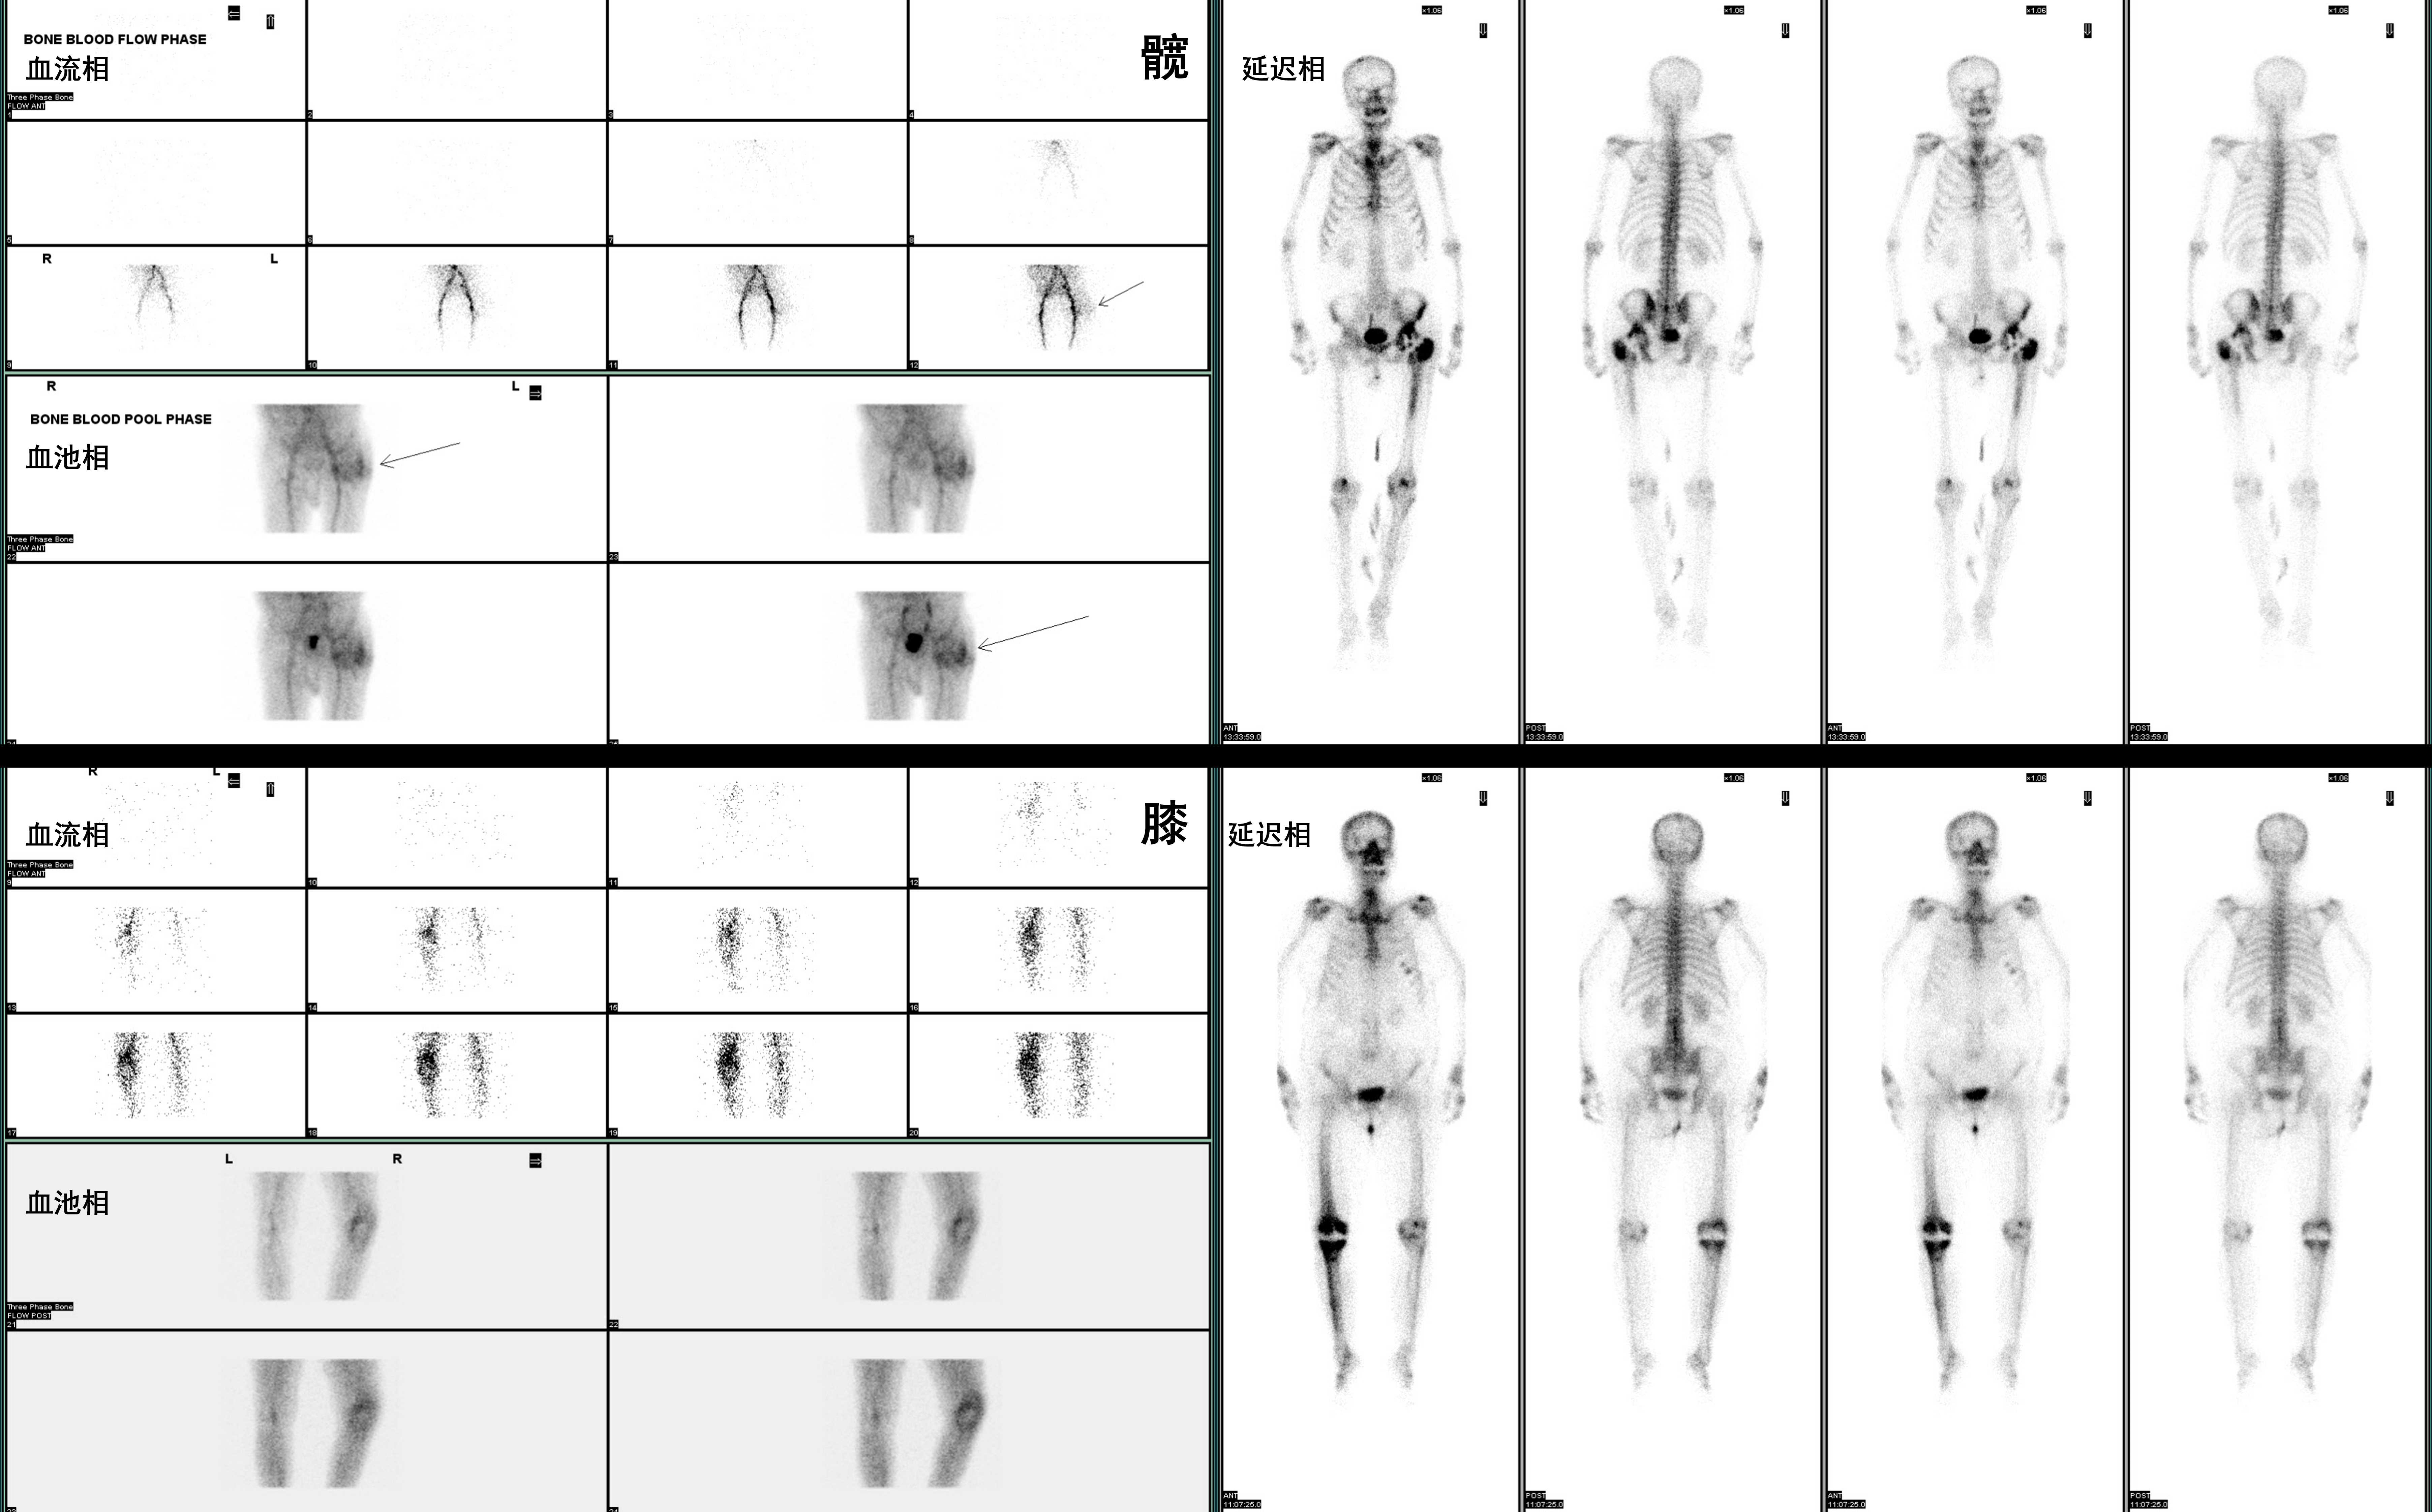
\includegraphics[width=\textwidth]{figures/chap01_DBS.png}
  \caption{\(^{99m}\)Tc-MDP 动态骨显像示意图}
  \label{fig:chap01_DBS}
\end{figure}

对于假体关节感染,核医学成像可以显示人工关节周围是否存在异常的代谢活动,揭示潜在的感染区域。如图\ref{fig:chap01_DBS},锝亚甲基二膦酸盐(\(^{99m}\)Tc-Methylene DiphosPhonate, \(^{99m}\)Tc-MDP)动态骨显像,也称之为骨三相,是核医学成像中第一个用于诊断假体关节感染的广泛可靠且简单影像模态\cite{niccoli2017bone}。Verberne等人\cite{verberne2016accuracy}的研究表明骨显像诊断全髋置换手术后的假体关节感染具有80\%的灵敏度和69\%的特异度。Kumar等人\cite{kumar2016comparative}发现动态骨显像在评估脓毒性的(或疼痛的)髋关节假体的敏感性、特异性和准确性分别为81\%、86\%和82\%。Zhang等人\cite{zhang2022temporal}通过在血流相中设定阈值的方法发现动态骨显像对膝关节假体感染的诊断灵敏度为94.3\%,特异度为56.0\%。根据文献和临床实践,动态骨显像诊断假体关节感染通常具有较高的敏感性,但特异性较低,尤其是经历过全膝置换手术的患者。

\begin{figure}[ht]
  \centering
  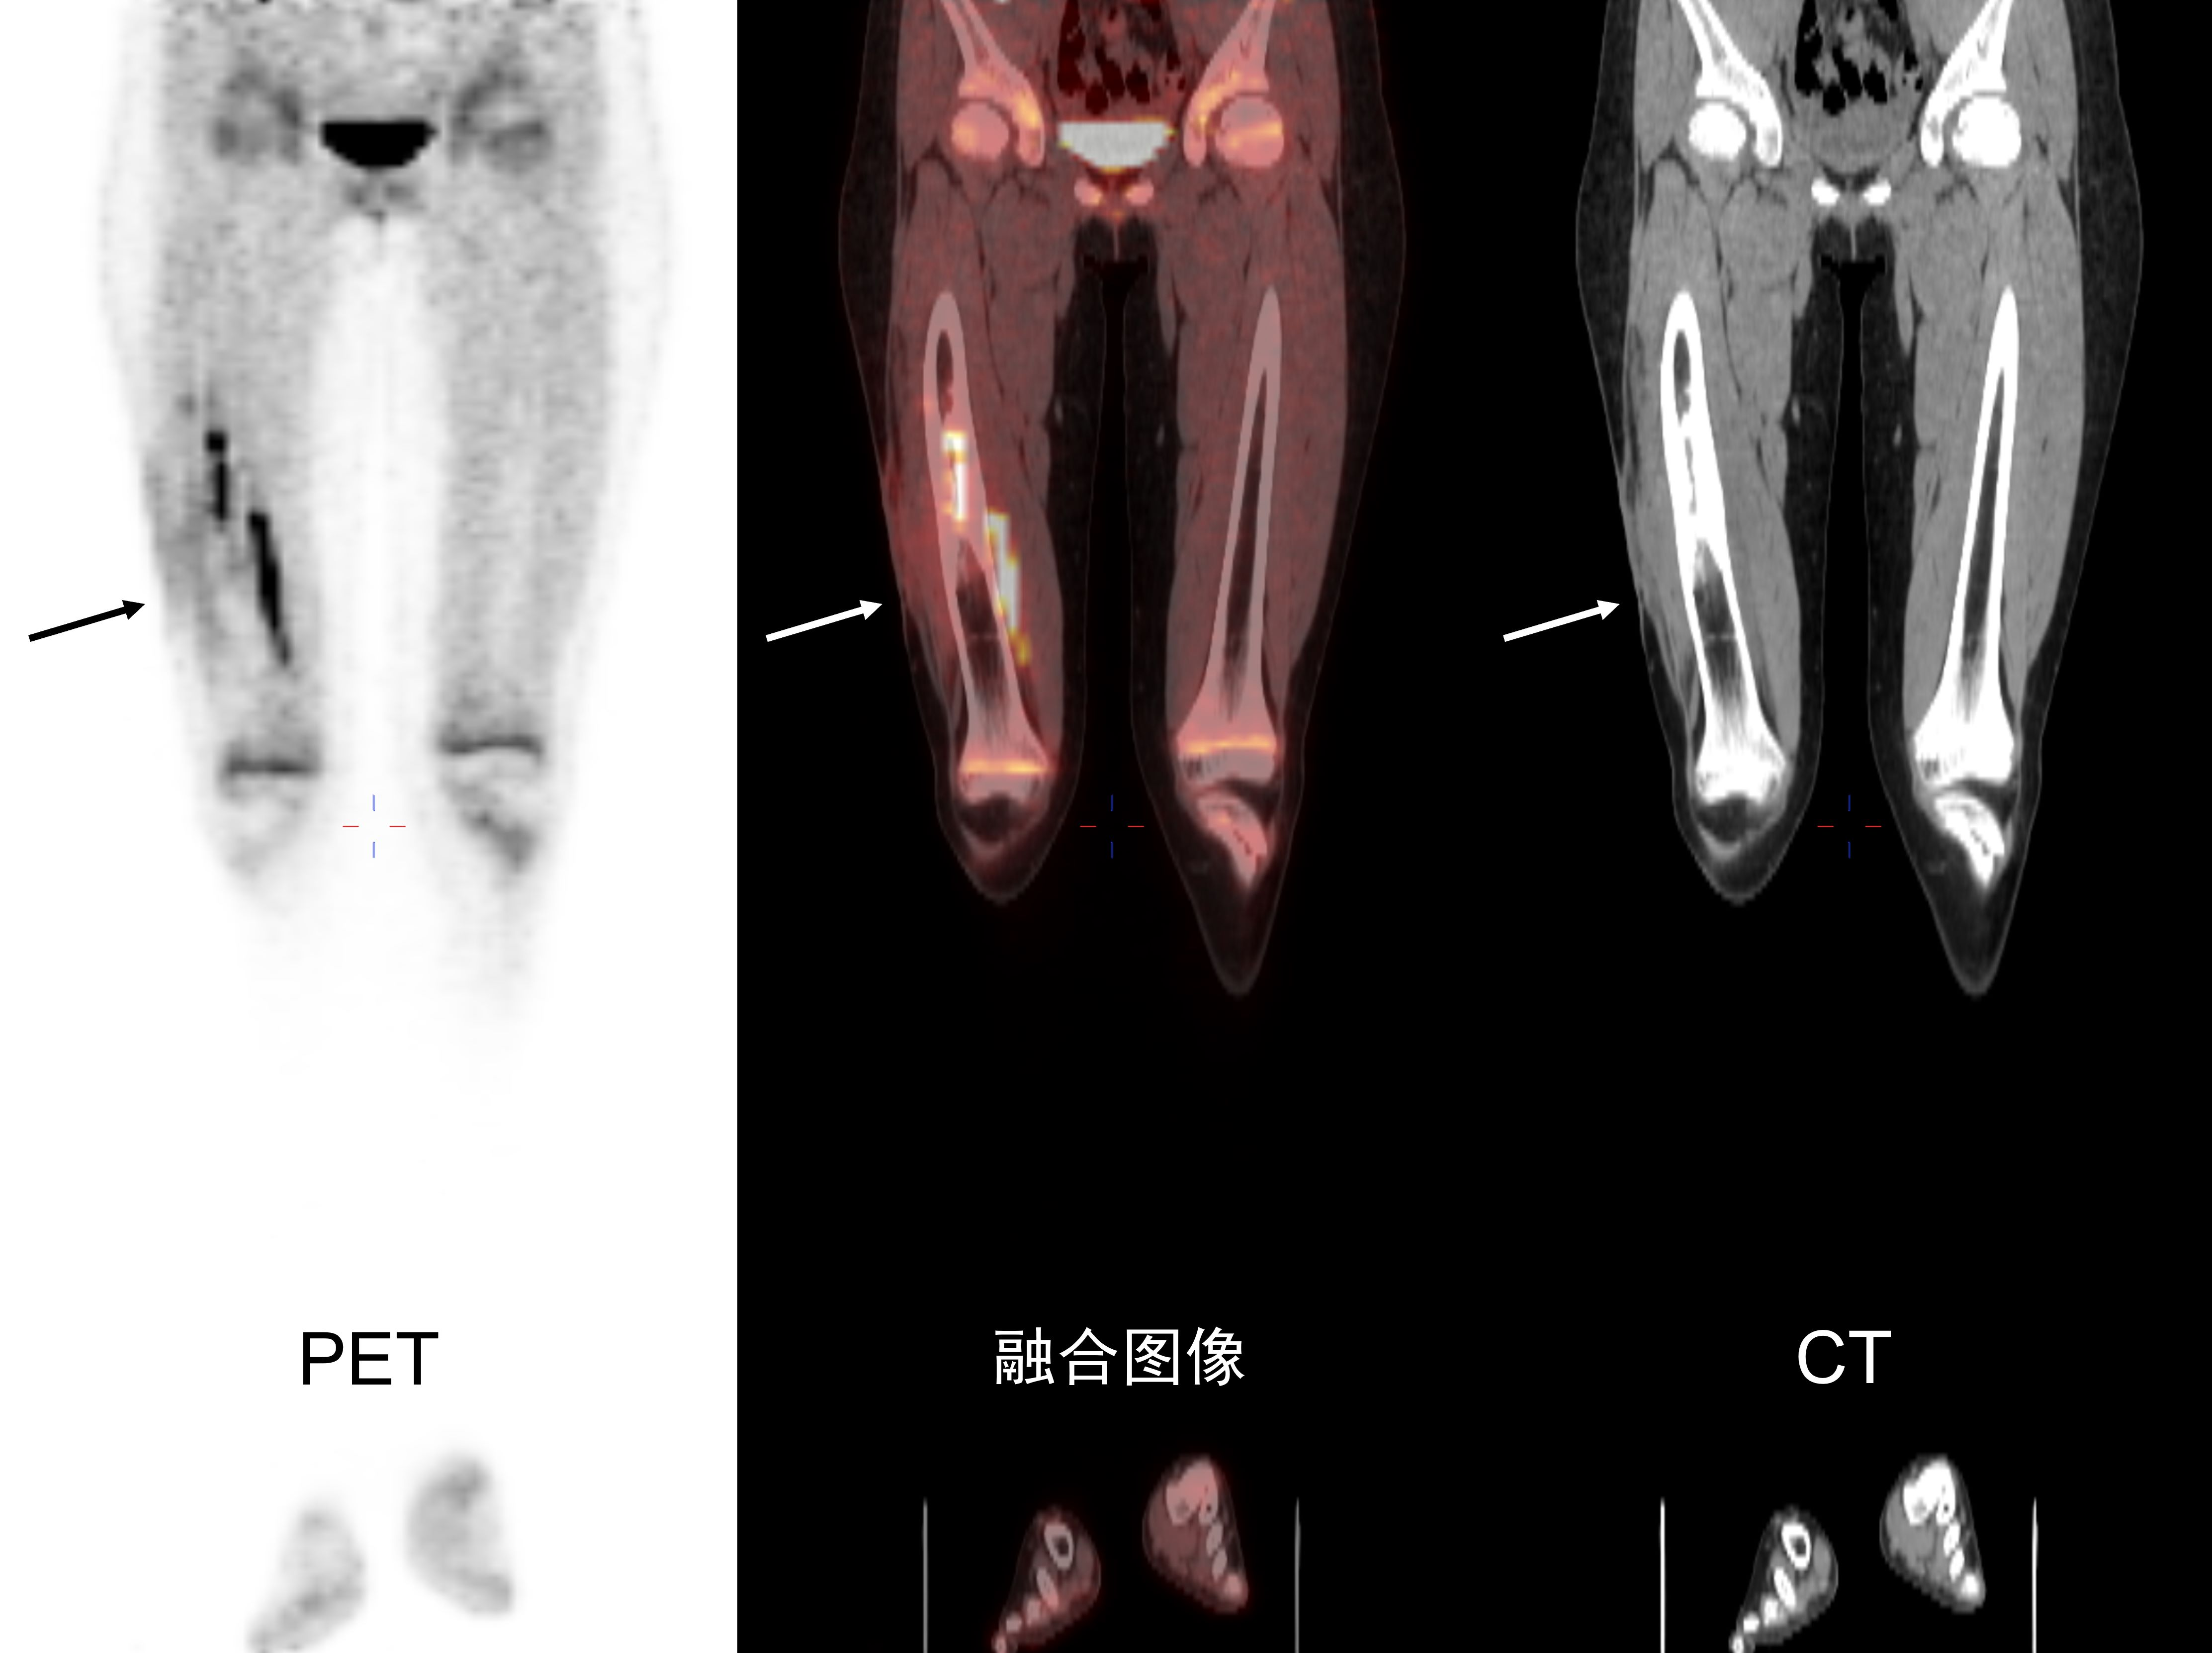
\includegraphics[width=0.8\textwidth]{figures/chap01_PETCT.png}
  \caption{\(^{18}\)F-FDG PET/CT示意图}
  \label{fig:chap01_PETCT}
\end{figure}

对于骨折相关感染,核医学成像则能够帮助定位骨折处是否存在感染迹象,有助于及早发现并采取适当的治疗措施。氟代脱氧葡萄糖(\(^{18}\)Fluorodeoxyglucose, \(^{18}\)F-FDG)PET/CT作为核医学的成像方式之一,常用于骨折相关感染的诊断\cite{zhang2021comparative},如图\ref{fig:chap01_PETCT}。它结合了解剖和生理信息,具有更高的空间分辨率和更好的量化可能性\cite{gholamrezanezhad2018clinical}。Lemans等人\cite{lemans2019diagnostic}通过在\(^{18}\)F-FDG PET/CT上量化分析,对骨折相关感染的准确率为83\%,阴性预测值为0.91。Wanter等人\cite{wenter2016diagnostic}研究发现,\(^{18}\)F-FDG PET/CT在慢性骨髓炎和骨科植入物相关感染中,阴性预测值为0.89、准确率为82\%。总体而言,\(^{18}\)F-FDG PET/CT在诊断骨折相关感染方面显示出令人满意的准确性。

近几年来,人工智能不断地发展,其在医学影像方面的应用也逐渐变成了关注的焦点。越来越多的深度学习方法被应用于医学影像领域的各种任务之中,如影像降噪,疾病分类,器官、组织和病灶的分割与检测、患者的预后效果预测等等\cite{ZSZD202307032,YJTY202304021}。以卷积神经网络(Convolutional Neural Network, CNN)、循环神经网络(Recurrent Neural Network,RNN)和基于注意力机制的Transformer为代表的深度学习方法因其优异的性能和较短的推理时间,经常被用来辅助核医学医生更迅速、准确地诊断病灶区域,减轻工作量。Liu等人\cite{liu2022diagnosis}提出了一种创新性多尺度CNN用于PET中阿尔茨海默病的诊断。Takahashi等人\cite{takahashi2022deep}提出了一个在PET/CT中对乳腺癌进行诊断的深度学习模型。然而,目前并没有用于假体关节感染和骨折相关感染这类骨科相关感染的自动化辅助诊断方法。为了有效地构建这种自动化辅助诊断方法,有几个问题必须前瞻性地加以考虑:

(1)数据集缺失。目前在网络上缺乏针对假体关节感染的动态骨显像数据集和针对骨折相关感染的PET/CT数据集。此外,医学影像数据集通常规模较小,来源相对单一,模型训练具有挑战性。

(2)髋关节的动态骨显像中存在生理上的高摄取区域,如膀胱和肾脏,这可能会使神经网络在进行预测时难以真正学习有用的信息并专注于病灶区域。其次,动态骨显像中包含血流相、血池相和延迟相(图\ref{fig:chap01_DBS}),且血流相和血池相中的图像序列具有时序性。因此,需要深入考虑如何充分利用动态骨显像的这些特点。最后,神经网络是一个缺乏解释的黑盒,这使得医生很难理解其预测的依据。

(3)尽管CT可以记录骨骼以及附近软组织的变化,但对骨折相关感染不太敏感。而PET中可以显示人体不同区域的代谢活性,且较高的标准摄取值反映了患有骨折相关感染的风险增加,但需要与炎症和愈合区分开来。其次,骨折相关感染的病灶区域仅占PET/CT整体影像的一小部分区域,且病灶的形状和位置多样,摄取的形式和程度也有所区别。因此,需要考虑到这些特征复杂性和多样性。最后,PET和CT都是三维的影像数据,这使得可以更全面地了解患者的解剖结构和生理活动。然而,这也给数据处理和模型设计带来了挑战。

(4)骨科相关感染的自动化辅助诊断方法应以简洁直观、易于操作的形式呈现,尤其对缺乏计算机和人工智能专业知识的用户尤为重要。首先,该方法需要整合骨骼感染的自动诊断流程,具备智能分析的能力,以协助医生更快速地做出准确的诊断决策。其次,该方法需要提供图形化界面,以方便用户操作。最后,医学影像的可视化是必不可少的功能之一,并且提供一些辅助功能,满足大多数医学影像模态的需求,以便用户可直观地阅览影像。

由此,本文提出了四个主要的研究目标:

(1)构建数据集,收集真实患者的假体关节感染或骨折相关感染的影像数据和诊断报告,并进行数据清洗、标注和预处理工作。

(2)设计一个在动态骨显像上基于深度学习的假体关节感染辅助诊断框架,自动得出诊断结果,并通过类激活图等方法给医生提供决策依据和可信度。

(3)设计一个在三维PET/CT上基于深度学习的骨折相关感染检测与诊断框架,从PET/CT中自动定位出病灶区域并判断出病灶区域是否存在感染。

(4)设计一个骨科相关感染的自动诊断与可视化方法,不仅提供智能化功能辅助非专业人员进行假体关节感染和骨折相关感染的自动诊断功能,还能够满足用户简单直观地阅览与分析医学影像。

\section{研究内容与创新点}

\begin{figure}[htbp]
  \centering
  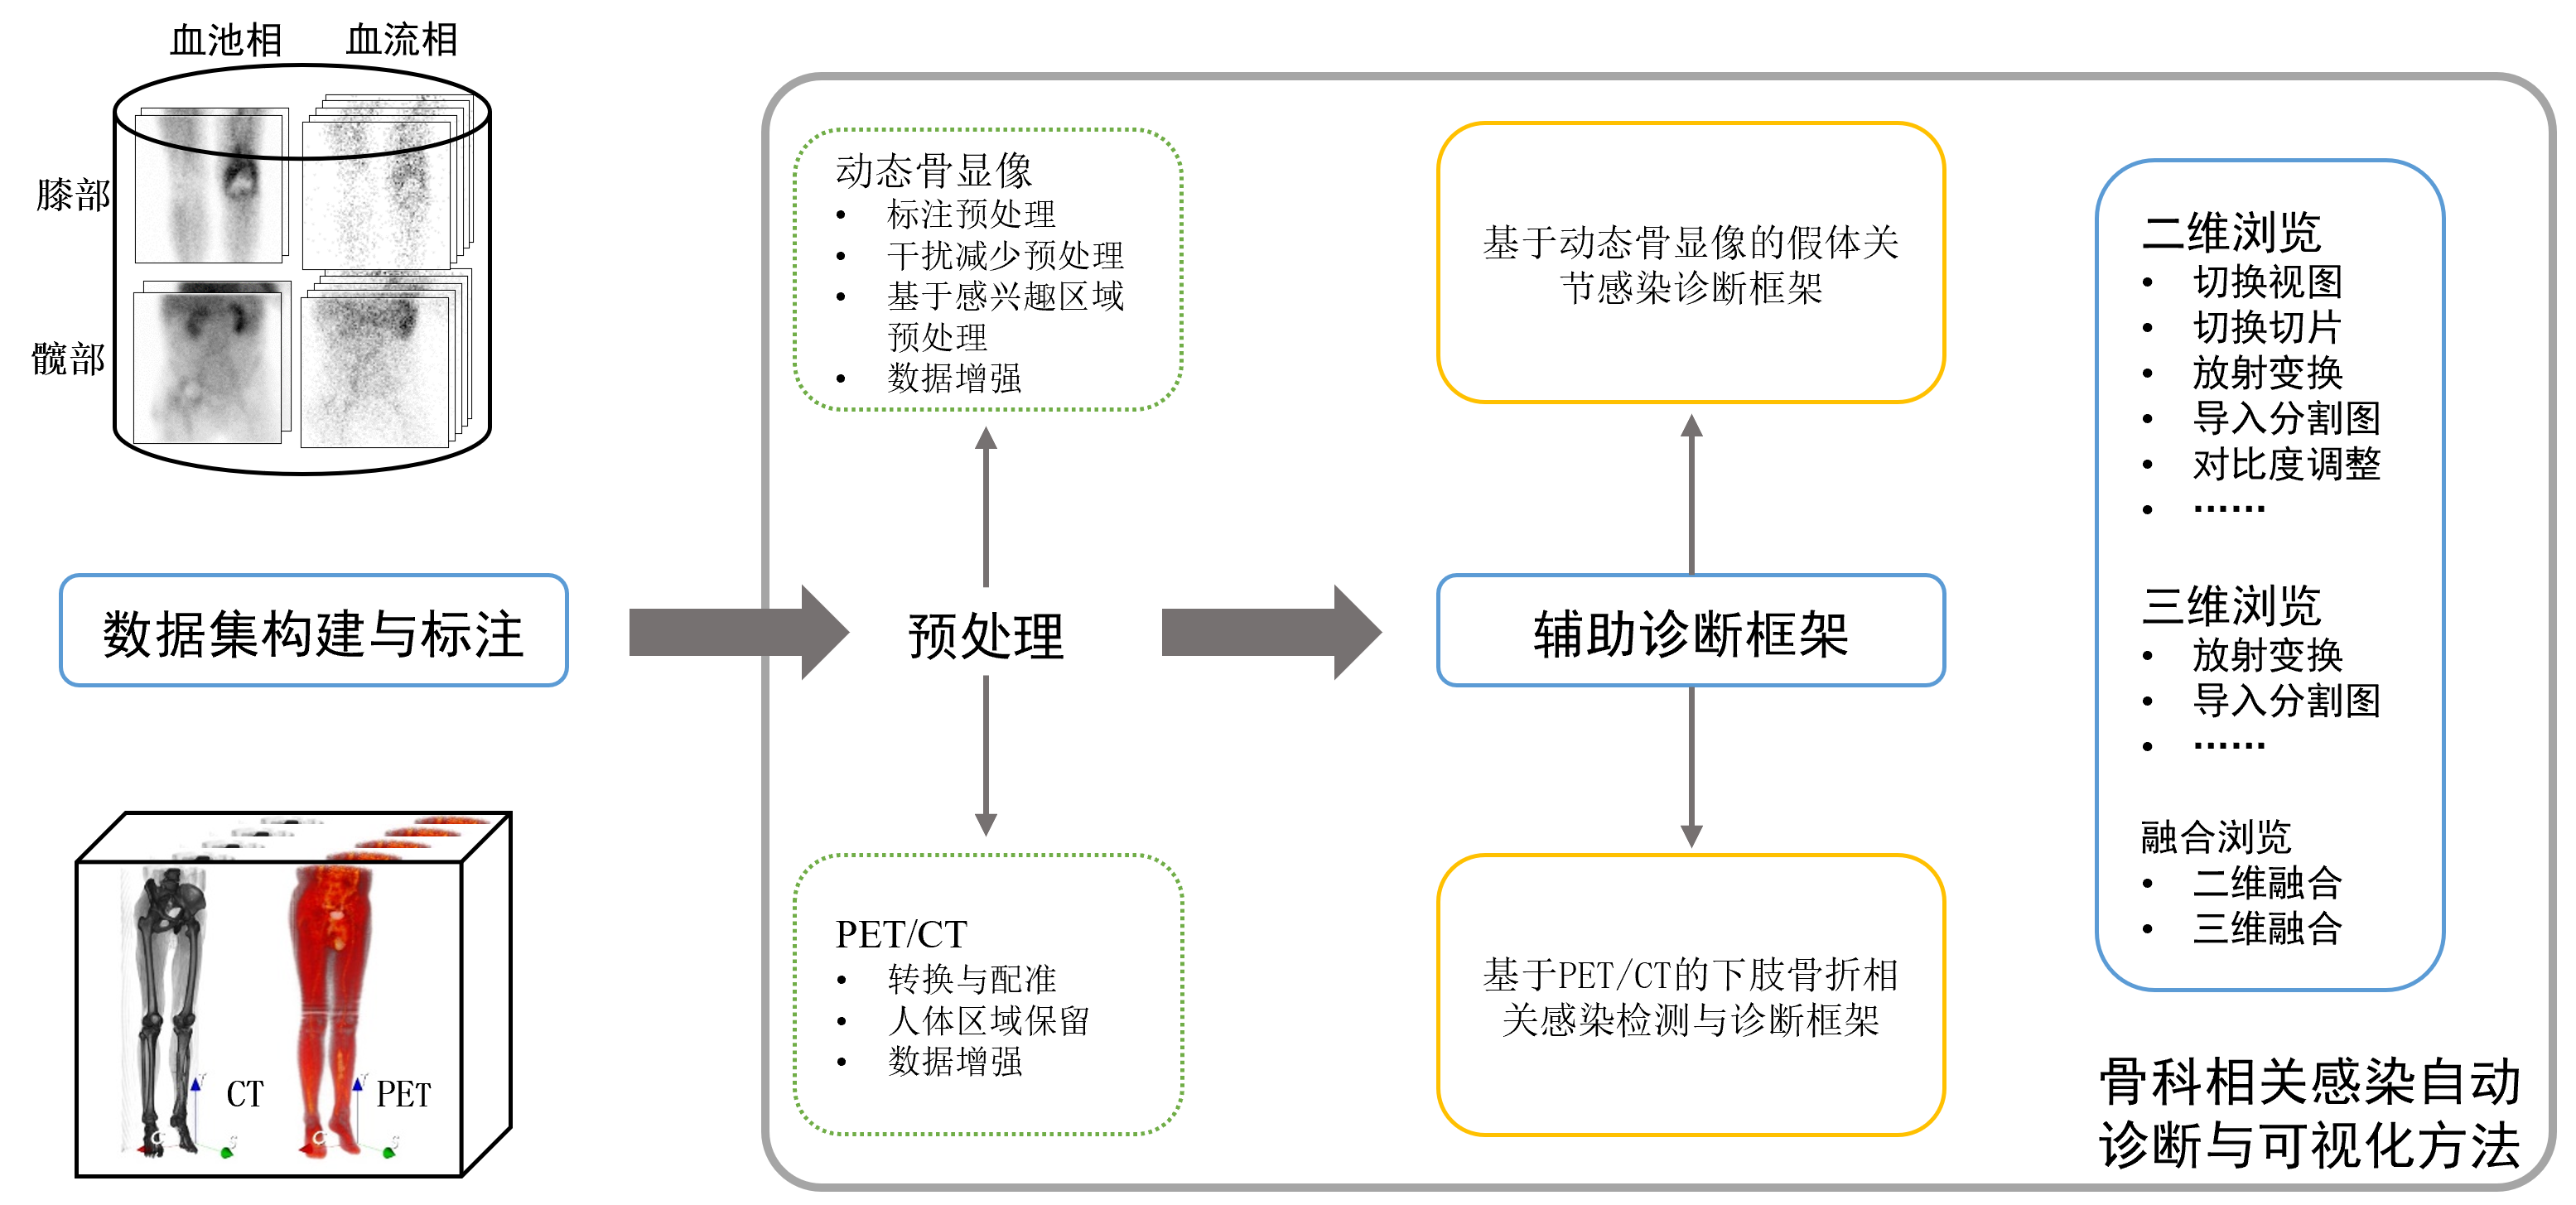
\includegraphics[width=\textwidth]{figures/chap01_research.png}
  \caption{本文的研究内容}
  \label{fig:chap01_research}
\end{figure}

根据1.2小节所述,本文围绕动态骨显像假体关节感染诊断分类任务、PET/CT骨折相关感染检测诊断任务以及骨科相关感染的可视化方法与自动诊断方法展开研究,主要研究内容和创新点如图\ref{fig:chap01_research}所示,包含以下四个部分:

(1)\textbf{数据集的构建与预处理方法的设计:}鉴于假体关节感染的动态骨显像数据集和骨折相关感染的PET/CT数据集的匮乏,本文作者与上海市第六人民医院核医学科合作,共同构建了两个重要的数据集。动态骨显像数据集纳入了在2016年1月至2021年6月期间455名患者的影像数据和相应的诊断报告,而PET/CT影像数据集则包含了2016年11月到2021年12月期间的281名患者的影像数据和诊断报告。在医学专家的指导下,通过仔细审查诊断报告和利用标注工具ITK-SNAP对数据集进行了详尽的标注工作,以确保数据的精准性和可靠性。针对动态骨显像和PET/CT影像,本文分别构建了一种高效的数据预处理方法。其中,动态骨显像采用了三种预处理算法和数据增强手段,而PET/CT影像则包括转换与配准、人体区域保留以及数据增强。这些预处理方法优化图像质量、标准化数据格式,并减缓无关区域和生理高摄取区域对模型性能的不良影响。

(2)\textbf{基于\(^{99m}\)Tc-MDP动态骨显像的假体关节感染辅助诊断框架:}为解决动态骨显像中假体关节感染诊断任务,构建了一种辅助诊断分类框架,由数据预处理和分类模型DBS-eNet组成。DBS-eNet结合了三维卷积和ConvLSTM,可以更有效地利用动态骨显像中不同相和相中的时序性图像序列。三维卷积用于在时序上提取不同相下每一张图像的生理摄取形态特征,ConvLSTM则捕捉和丰富单一图像的生理形态摄取特征,同时捕获图像序列中生理代谢的差异变化特征。实验结果表明,在五折交叉验证中,该框架在假体膝关节感染和假体髋关节感染的诊断任务上优于其他CNN,分类准确率分别达到了86.48\%和86.33\%;在独立验证中,该框架在假体膝关节感染上分类准确率达到了87.74\%,相比核医学专家们提升了13.55\%;在假体髋关节感染上分类准确率达到了86.36\%,与核医学专家们一致。统计学分析表明,该框架的诊断性能在假体膝关节感染上优于核医学专家,在假体髋关节上与核医学专家相当。

(3)\textbf{基于\(^{18}\)F-FDG PET/CT三维影像的下肢骨折相关感染检测与诊断框架:}为解决PET/CT影像中下肢骨折相关感染诊断任务,本文提出了一种全自动两阶段的检测与诊断框架3DFRINet。其中,3DFRINet 由病灶检测网络和病灶诊断分类网络构成。通过双分支设计和注意力模块,病灶检测网络能够捕获和融合不同模态的多尺度细节特征,从而精准地检测出病灶区域。病灶诊断分类网络通过最大强度投影将立体影像转换为平面图像,在获取有效特征的同时,对候选区域进行进一步挖掘,以捕捉骨折相关感染的代谢形态特征,从而实现对其准确的分类。实验结果表明,3DFRINet在下肢PET/CT影像中病灶检测性能优于其他YOLO模型,其AP\(_{25}\)达到了0.9234。在骨折相关感染病灶诊断分类任务中,该方法上达到了91.55\%的分类准确率和0.9250的F1,相比较于与初级核医学医生分别提升了11.27\%和0.1045,比高级核医学医生分别提升了4.32\%和0.0419。统计学分析表明,3DFRINet具有与初级核医学医生更好或相同的诊断能力,与高级核医学医生相当的诊断性能。

(4)\textbf{骨科相关感染的自动诊断与可视化方法:}为了构建一个假体关节感染和骨折相关感染的自动化辅助诊断方法,本文采用PyQt6框架,设计了一个骨科相关感染的自动诊断与可视化方法。该方法旨在为医生提供一款功能强大的辅助工具,具备全面而便捷的影像阅览和智能分析功能。在智能分析方面,该方法整合了(2)和(3)中的框架,以支持假体关节感染的诊断分类和骨折相关感染的病灶自动检测和分类。在影像阅览方面,该方法支持二维、三维和融合可视化,以满足不同医学影像模态的需求。二维可视化兼容大多数医学影像模态,提供显示视图、坐标和所在坐标值的信息,切换视图、几何变换等功能;三维可视化仅支持PET和CT,提供了旋转、缩放等功能;融合可视化支持PET和CT融合阅览,提供了二维和三维可视化功能。

\section{本文的整体结构}

本文基于作者攻读硕士学位期间的研究方向和参与的课题,分为六个章节,如图\ref{fig:chap01_structure}所示。各章节的内容安排如下:

\begin{figure}[htbp]
  \centering
  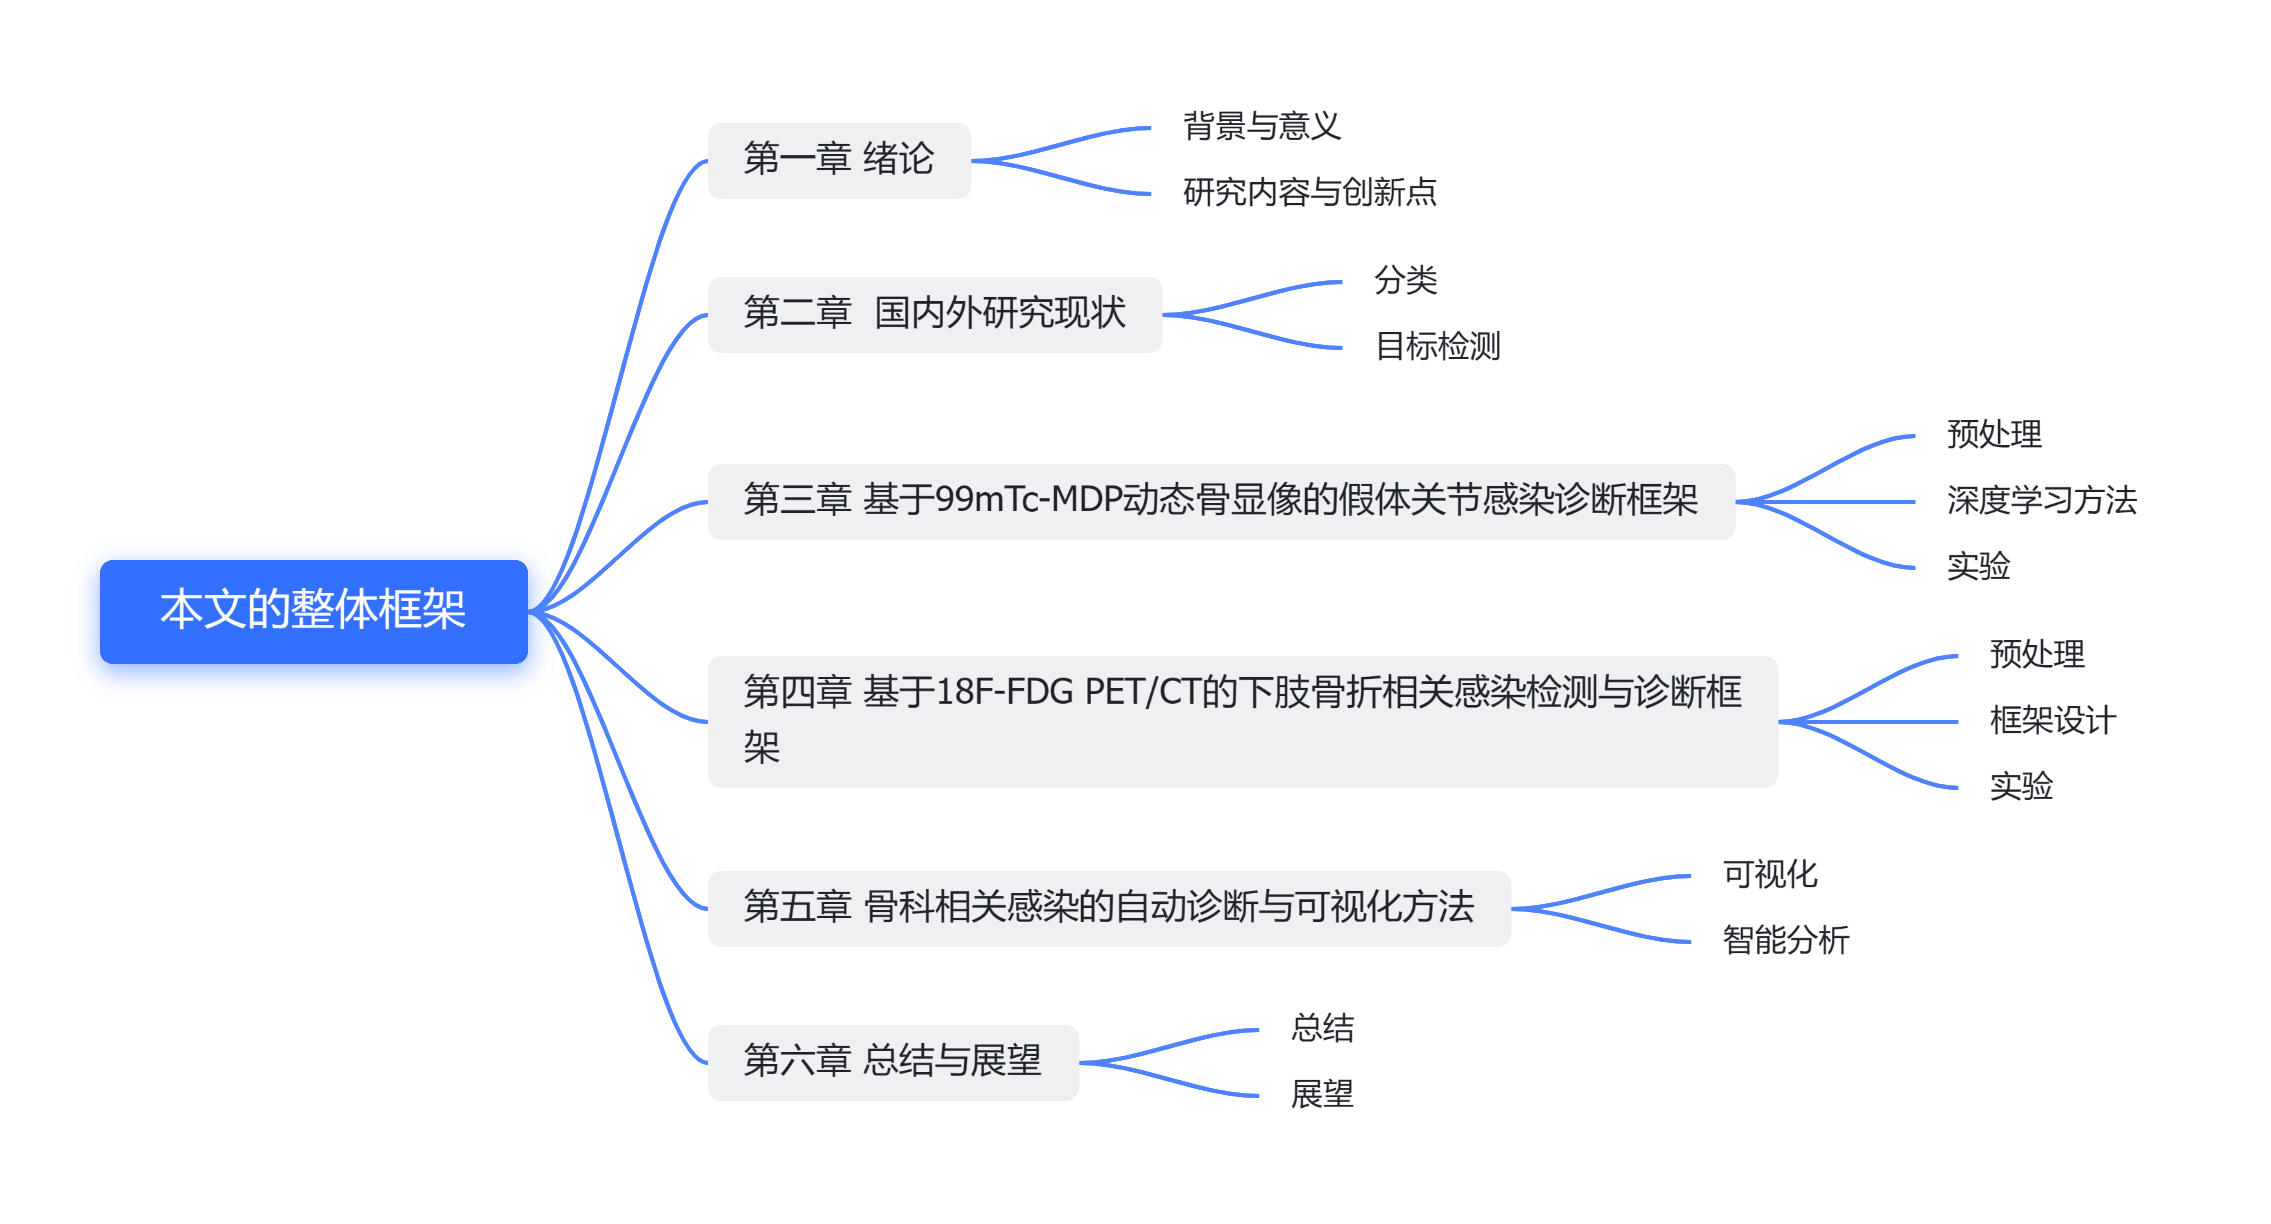
\includegraphics[width=\textwidth]{figures/chap01_structure_light.png}
  \caption{论文的整体结构}
  \label{fig:chap01_structure}
\end{figure}

第一章详细介绍了假体关节感染和骨折相关感染。接着阐述了深度学习方法与医学影像结合在骨科相关感染自动诊断方面的研究背景和研究意义,并介绍了研究的内容、目标和创新点。

第二章介绍了与本文研究内容相关的近几年国内外相关工作,总结了目前医学影像中分类和检测任务的研究进展,最后阐述了本文中假体关节感染和骨折相关感染诊断任务的特点,总结了任务的特殊性和现有的可行方法。

第三章从问题定义出发,详细介绍了基于\(^{99m}\)Tc-MDP动态骨显像的假体关节感染诊断框架。内容包括数据预处理方法、深度学习方法中模型的整体结构、损失函数以及用于展示模型可解释性的可视化方法。接着,通过一系列实验评估了该诊断框架的有效性和较好的诊断性能。

第四章同样从问题定义入手,详细介绍了基于\(^{18}\)F-FDG PET/CT三维影像的下肢骨折相关感染检测与诊断框架。内容包括数据预处理方法和框架设计。随后,通过一系列实验评估了该框架在病灶检测和诊断方面的出色表现。

第五章详细地介绍了骨科相关感染的自动诊断与可视化方法,拥有智能影像分析与影像阅览功能。该方法支持不同医学影像模态的可视化功能,还整合了第三章和第四章的辅助诊断框架。该方法不仅是实用的辅助工具,更是与自动化诊断方法交互的桥梁,为医学影像分析提供了有力支持。

第六章对本文的研究工作进行了总结,并提出了未来可以进一步研究的方向。












% !Mode:: "TeX:UTF-8"
\chapter{国内外研究现状}\label{chap:related_work}

本章旨在综述国内外关于本文研究内容的相关工作。首先,本章将介绍当前计算机视觉领域中与分类和检测任务相关的神经网络模型。特别地将重点介绍并分析分类任务中的CNN系列、Transformer系列和RNN系列模型和在检测任务中的U-Net系列目标分割模型、R-CNN和YOLO系列目标检测模型。其次,本章将详细介绍医学影像领域中分类任务与检测任务的最新研究进展,并对本文所涉及的假体关节感染和骨折相关感染诊断任务的特殊性和现有方法进行深入分析与总结。

\section{图像分类}

分类任务是指输入数据经过模型计算后分为不同的类别或者标签的任务,这是深度学习中最常见和最基本的问题之一。其中,模型需要从训练数据集中学习数据特征与标签之间的关系,用以对未见过的数据正确地从已知的多个标签集合中选择最合适的一个或几个标签。在计算机视觉领域中,对图像、视频或其他视觉数据的特征提取一直以来都是研究的核心问题。赋予计算机类似于人类一样的智慧视觉能力是多年来许多研究人员共同追求的目标和努力方向。随着相关技术的不断发展,尤其是图像识别技术的不断进步,在计算机视觉领域之中的分类任务在医疗、航海、交通等多个现实场景中有着诸多良好的应用前景,包括人脸识别、航空遥感和医学影像等等。

通常情况下,分类任务的主要流程包括特征提取和模型设计两个关键步骤。合适的特征提取和模型设计可以相辅相成,以实现较优异的性能表现。在早期,图像识别技术\cite{fu1976pattern}主要采用了基于先验知识设计的手工特征。原理在于对于不同的应用场景,需要由相应领域的专家提供专业知识去设计所需要的特征。然而,这种针对某一的领域特性和相应的数据类型进行的手工编码,难以去处理海量的数据,效率及其低下\cite{季长清2022基于卷积神经网络的图像分类算法综述}。此外,人工设计的特征的普遍性不强,图像中可能存在噪声,难以涵盖所有情形,很可能导致分类的结果并不理想。而在图像领域中,常见的形状、纹理、颜色等浅层视觉特征和局部二值模式、方向梯度直方图等局部不变特征,虽然具有一定的普适性,但应用到现实场景具体图像时,针对性不足,尤其是面对一些存在复杂场景的情形,更加难以去准确使用手工特征去描述目标图像\cite{杨真真2018基于卷积神经网络的图像分类算法综述}。

在模型方面,传统的机器学习模型实现简单,决策依据直观可理解,但对于复杂图像如图像噪声干扰较多,不同类别之间差异小等问题,其性能会大大下降。此外,传统机器学习依赖于特征提取,难以实现全自动化,性能极大受限于手工特征的有效性。随着计算机硬件的快速发展,特别是图形处理器(Graphics Processing Unit,GPU),以及大规模训练数据集(ImageNet\cite{deng2009imagenet}、CelebA\cite{liu2018large}等)的出现,深度学习方法在计算机视觉领域中其优越性在不断凸显。相比较于传统的图像识别技术,深度学习方法不再需要人工设计的手工特征,而是通过神经网络模型自主地在训练数据集中学习到潜在有效的特征,这很好地将特征提取融合到模型设计之中,解决了人工设计特征的难题。由此,深度学习方法开始逐步替代传统的机器学习方法成为了主流,得到了飞跃式的进展。

本文围绕动态骨显像和PET/CT进行相关研究。由于动态骨显像和PET/CT的特点,导致难以直接应用深度学习方法进行影像特征提取。例如,动态骨显像和PET/CT都是单通道的图像数据,以强度的大小与分布来进行表示。其中,动态骨显像与PET可以展示人体组织生理代谢的强弱,而CT可以展示人体组织的解剖结构信息。影像中的无关区域与干扰区域会影响最终分类的精度,且单独的图像特征并不充足。动态骨显像还具有时序上的特征;而PET/CT还具有更全面的立体特征。

\subsection{图像分类算法}

常见的机器学习模型有K-近邻算法,决策树、支持向量机等等。K-近邻算法(K-Nearest Neighbor,KNN)\cite{guo2003knn}基于一个简单的假设:相似的样本具有相似的标签。该算法通过计算样本之间的距离来代表样本之间的相似性,在训练数据集中根据每个未知样本最相似的K个邻居来对该未知样本进行分类。该算法简单直观易于理解,但计算和内存的开销大且对不平衡数据集不友好。决策树\cite{suthaharan2016decision}的基本思想是通过一系列的对某一特征值的条件筛选来对数据进行划分,直至划分到叶子结点得到最终的预测结果。该算法易于理解和解释,具有可视性,但容易过拟合和达到局部最优解。支持向量机(Support Vector Machine,SVM)\cite{suthaharan2016support}的基本思想是寻找一个可以将不同类别样本隔开的超平面,并且最大化样本与超平面之间的最小距离。该算法具有较强的泛化能力和对噪声的鲁棒性,但仅适用于二分类问题,且计算和内存的开销大。

\begin{figure}[h]
  \centering
  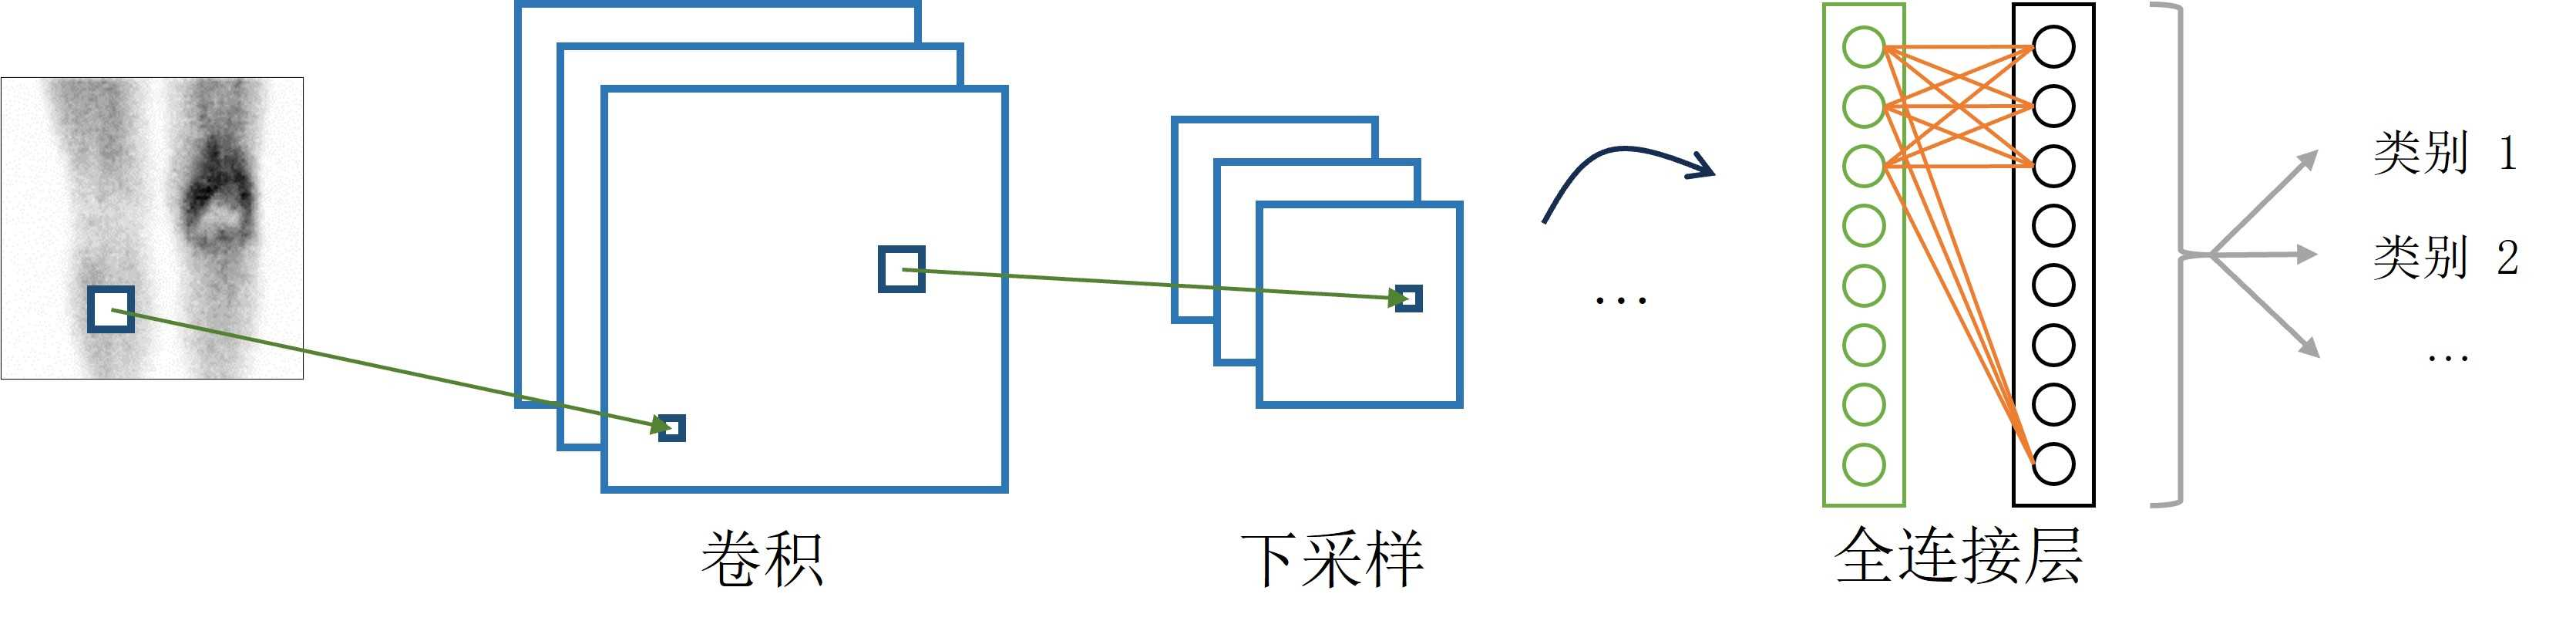
\includegraphics[width=\textwidth]{figures/chap02_cnn.jpg}
  \bicaption{卷积神经网络示意图}{Schematic of the convolutional neural network}
  \label{fig:chap02_cnn}
\end{figure}

如今,深度学习方法逐渐成为主流,逐步取代了传统机器学习方法的地位。CNN是深度学习方法中具有代表性的方法之一,通常由卷积层,下采样层,全连接层组成,如图\ref{fig:chap02_cnn}所示。卷积层是核心组成部分,最大的特点在于参数共享机制,即通过相同的参数提取输入数据中不同位置的同一特征。参数共享机制可以大大减少参数的数量,提高模型的泛化能力。卷积层中若干个卷积核都具有可学习的参数,而该参数通过梯度反向传播算法进行训练调整。对于输入到卷积层的二维矩阵数据\(I\)而言,输出的像素点\(O_{i,j}\)可由公式\ref{eq:chap02_convolution}表示:
\begin{equation}
  O_{i,j} = \sum_{m=0}^{M-1}\sum_{n=0}^{N-1}I_{i+m, j+n}\times K_{m,n}
  \label{eq:chap02_convolution}
\end{equation}
其中,\(i,\ j\)表示输出矩阵的位置,\(M,N\)是二维卷积的尺寸大小,\(K_{m,n}\)表示卷积核中的权重值。其中,输出图像\(O\)每个位置的值,由卷积核\(K\)会沿着二维矩阵数据\(I\)进行窗口滑动依次计算得出。

接下来将介绍与分析一些经典的CNN模型:LeNet\cite{lecun1998gradient}(1998)是历史上第一个成功应用于手写数字识别任务的CNN,并且为后来的更深层次的CNN的发展奠定了基础。LeNet的整体结构非常简单,一共有七层,包括交替的卷积和池化层,以及全连接层和输出层。它的成功证明了CNN在图像识别任务上的有效性,也使得它成为深度学习领域中里程碑式的模型之一。

AlexNet\cite{krizhevsky2012imagenet}(2012)可以视为第一个现代深度CNN模型,与LeNet有着相似的网络结构,但网络层数更深。它的主要贡献在于:(1)引入了ReLU激活函数去加速训练过程并减轻了梯度消失问题。(2)为了减少过拟合,引入了Dropout\cite{srivastava2014dropout}正则化技术和数据增强方法用以提升模型的泛化能力和鲁棒性并扩充了数据集的大小。AlexNet的出现为后续的CNN的设计和训练提供了重要的启发和借鉴。

VGG\cite{Simonyan2014VeryDC}(2014)的网络结构简单而有效。与AlexNet相比较,它的卷积核更小,都是\(3\times3\)的大小。这不仅可以减少模型参数量,还增加了模型的非线性能力。此外,VGG的网络结构可以更深,通常为16或19层,这使得网络可以捕获更好的复杂特征。VGG在图像分类任务上取得了很大的成功,其清晰的网络结构和易于理解的设计使得它成为了深度学习入门的经典模型之一。

\begin{figure}[ht]
  \centering
  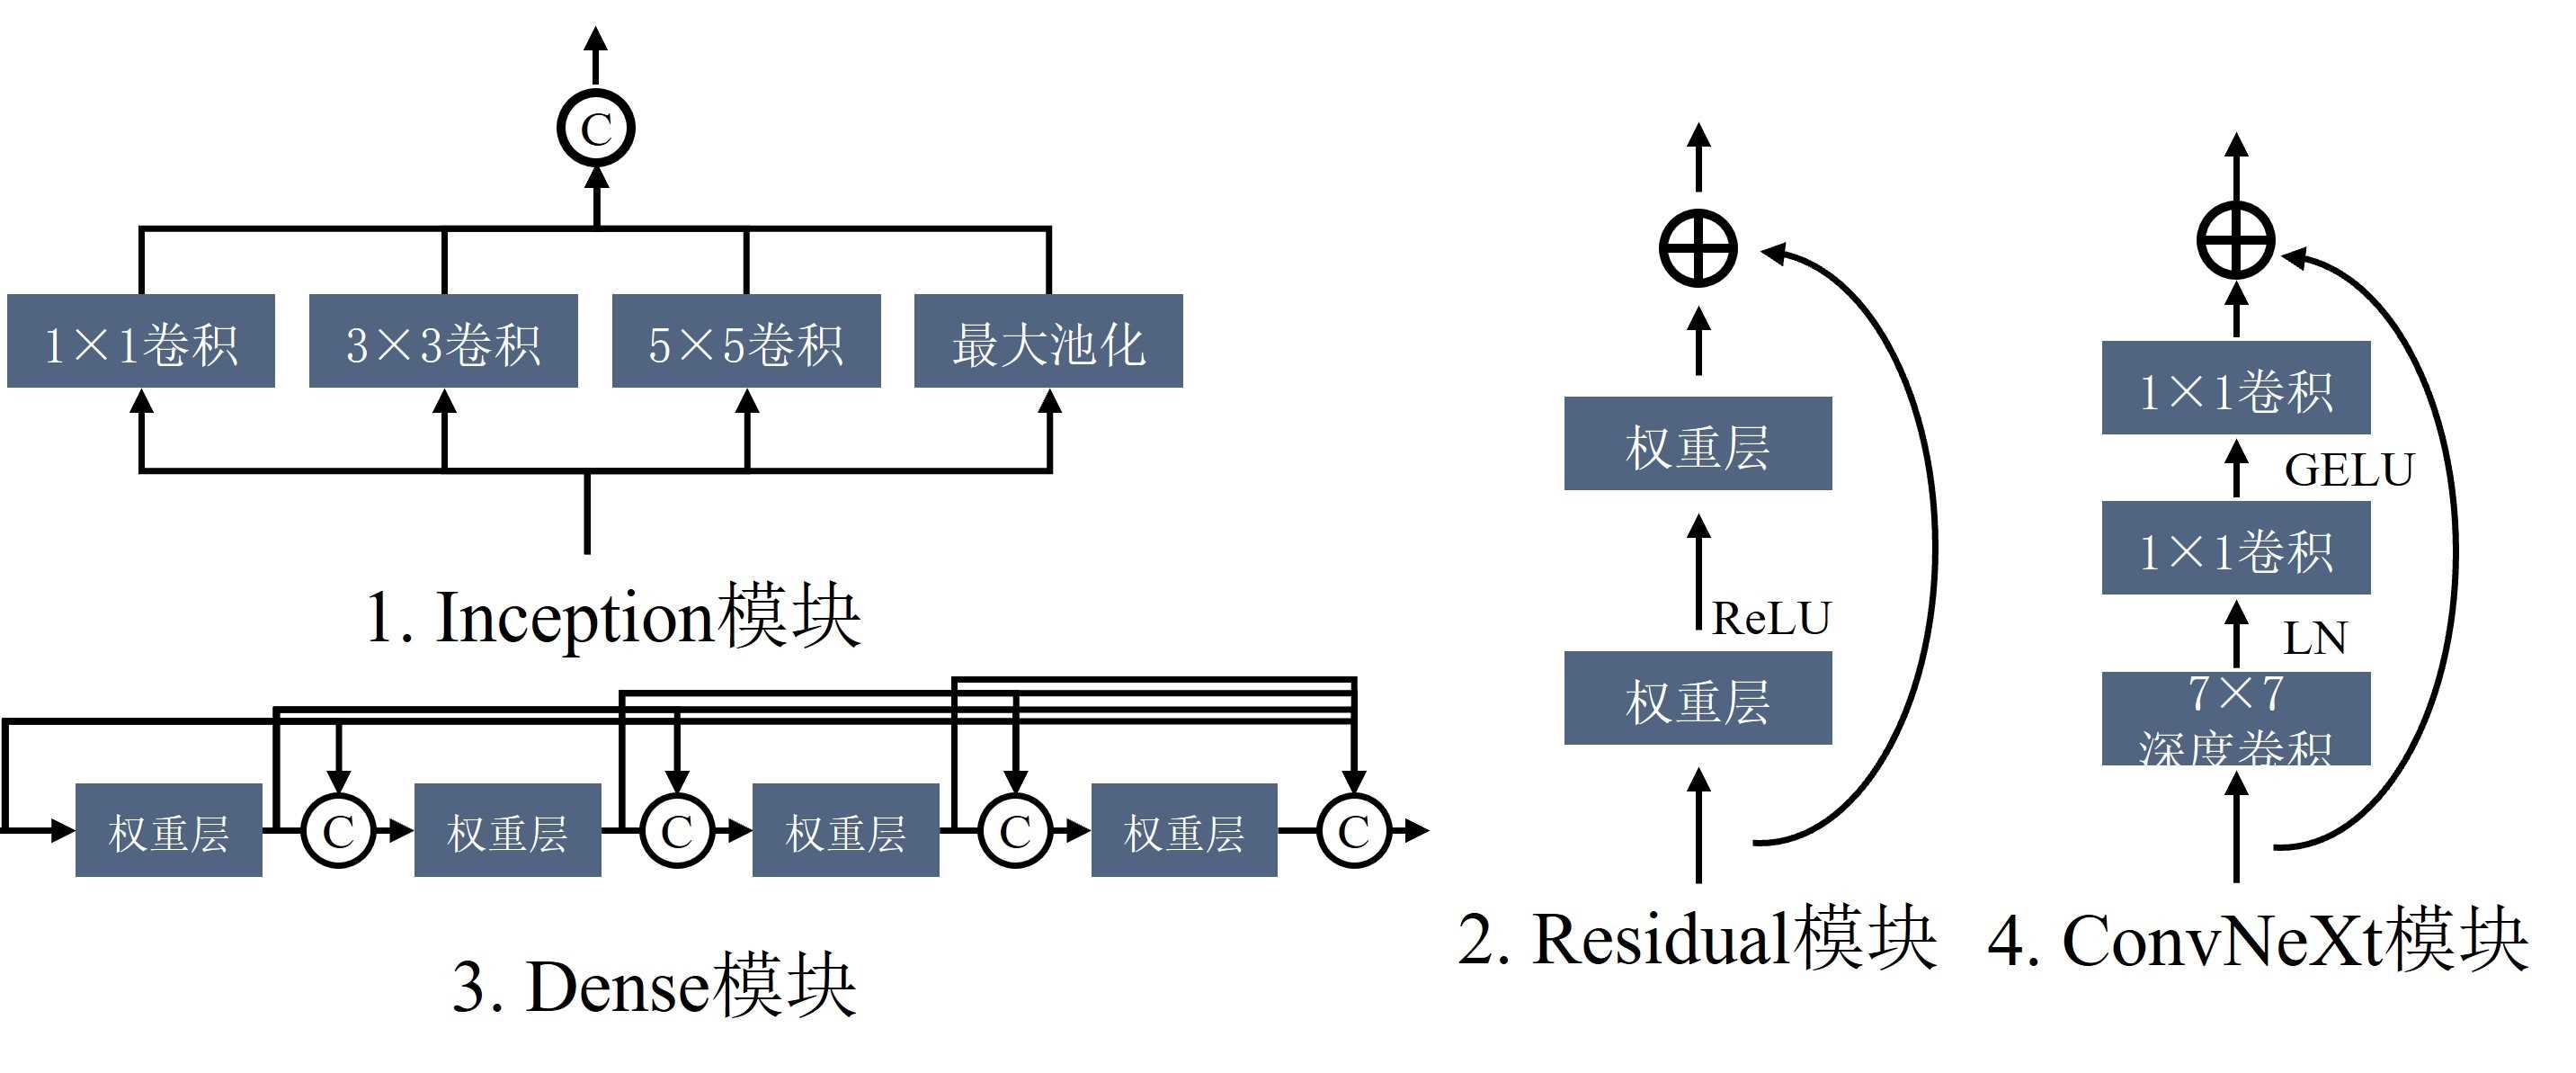
\includegraphics[width=\textwidth]{figures/chap02_block.jpg}
  \bicaption{不同卷积神经网络的模块示意图}{Schematic of the modules of different convolutional neural networks}
  \label{fig:chap02_block}
\end{figure}

GoogleNet\cite{szegedy2015going}(2014),也称为Inception网络,初次引入了基础模块(Inception模块,图\ref{fig:chap02_block})的概念,用以搭建一个稀疏且高性能的神经网络模型。Inception模块采用高度并行的设计方式,在多个不同尺度上同时执行卷积和池化操作,以捕获不同层次的特征。它将不同大小的卷积核和池化核组合在一起,让神经网络模型自主学习最合适的特征提取方式。尽管GoogleNet的网络结构为22层,但它的参数量是AlexNet的1/15,同时是VGG的1/3。因此,GoogleNet是在计算资源有限的情况下的一个较好选择。此外,GoogleNet使用全局平均池化层替代了全连接层来整合特征,将每个特征图转换为一个单独的特征值,在大大减少参数量的同时降低了过拟合的风险。

ResNet\cite{he2016deep}(2015)的核心创新点在于引入了Residual模块(图\ref{fig:chap02_block}),用以解决神经网络层数加深时出现的问题,如梯度爆炸、梯度消失以及神经网络模型能力退化。其中,模型能力退化并不是由过拟合造成的,而是由于模型层数的增加导致训练误差的增加。从LeNet到GoogleNet模型发展的历程来看,神经网络模型的网络结构越深,意味着可以提取到越丰富的特征,并且,在更深的网络结构下提取的特征图含有更充足的语义信息。但是实验表明随着神经网络模型不断加深,模型的性能越差。Residual模块通过引入跳跃连接的方式,即将浅层的输入直接与深层的输出相加,保持梯度的流动,提升信息的传播效率,来解决梯度和训练困难的问题。ResNet可以构建非常深的网络,甚至可以超越1000层。相比于传统的网络模型,ResNet更容易优化和训练。ResNet也是深度学习领域中里程碑式的成果之一。

DenseNet\cite{huang2017densely}(2017)在ResNet的基础上更进一步,充分利用了跳跃连接,提出了具有密集连接的Dense模块,如图\ref{fig:chap02_block}。Dense模块为了确保信息的最大流动,将所有层相互连接,其中每个卷积层的输入是前面所有层的特征图拼接而成,输出会保留下来并传给后面所有的层进行拼接。这种密集连接的设计使得网络可以更充分地利用前面提取的特征信息,提升网络模型的表达能力,也有助于解决梯度消失和信息稀疏的问题。DenseNet通过密集连接的设计,实现了全局特征的重用,从而提高了网络对复杂特征的捕获能力。其创新的网络结构和有效的特征融合方式丰富了深度学习模型的设计空间,提供了新的研究思路与方法。

ConvNeXt\cite{liu2022convnet}(2022)从ResNet模型出发,在Swin Transformer\cite{liu2021swin}的设计启发中汲取精华,在网络结构和训练策略上进行了多项改进,得到了性能超越Swin Transformer的CNN。ConvNeXt的基础模块如图\ref{fig:chap02_block}所示。由于Swin Transformer采用较大的自注意力窗口,自注意力中中间隐藏层的特征图通道数更大并且深度可分离卷积与注意力机制的计算具有相似性,ConvNeXt模块采用了倒置瓶颈结构,即中间大、两头小,并使用了大卷积核(\(7\times7\))的深度可分离卷积。此外,在细节优化上,将激活函数ReLu改为了GELU,归一化函数Batch Normalization\cite{ioffe2015batch}改成了Layer Normalization。ConvNeXt表明了纯粹的CNN经过精心设计,依然可以与以Transformer为代表的新兴模型展开竞争。

\begin{figure}[htbp]
  \centering
  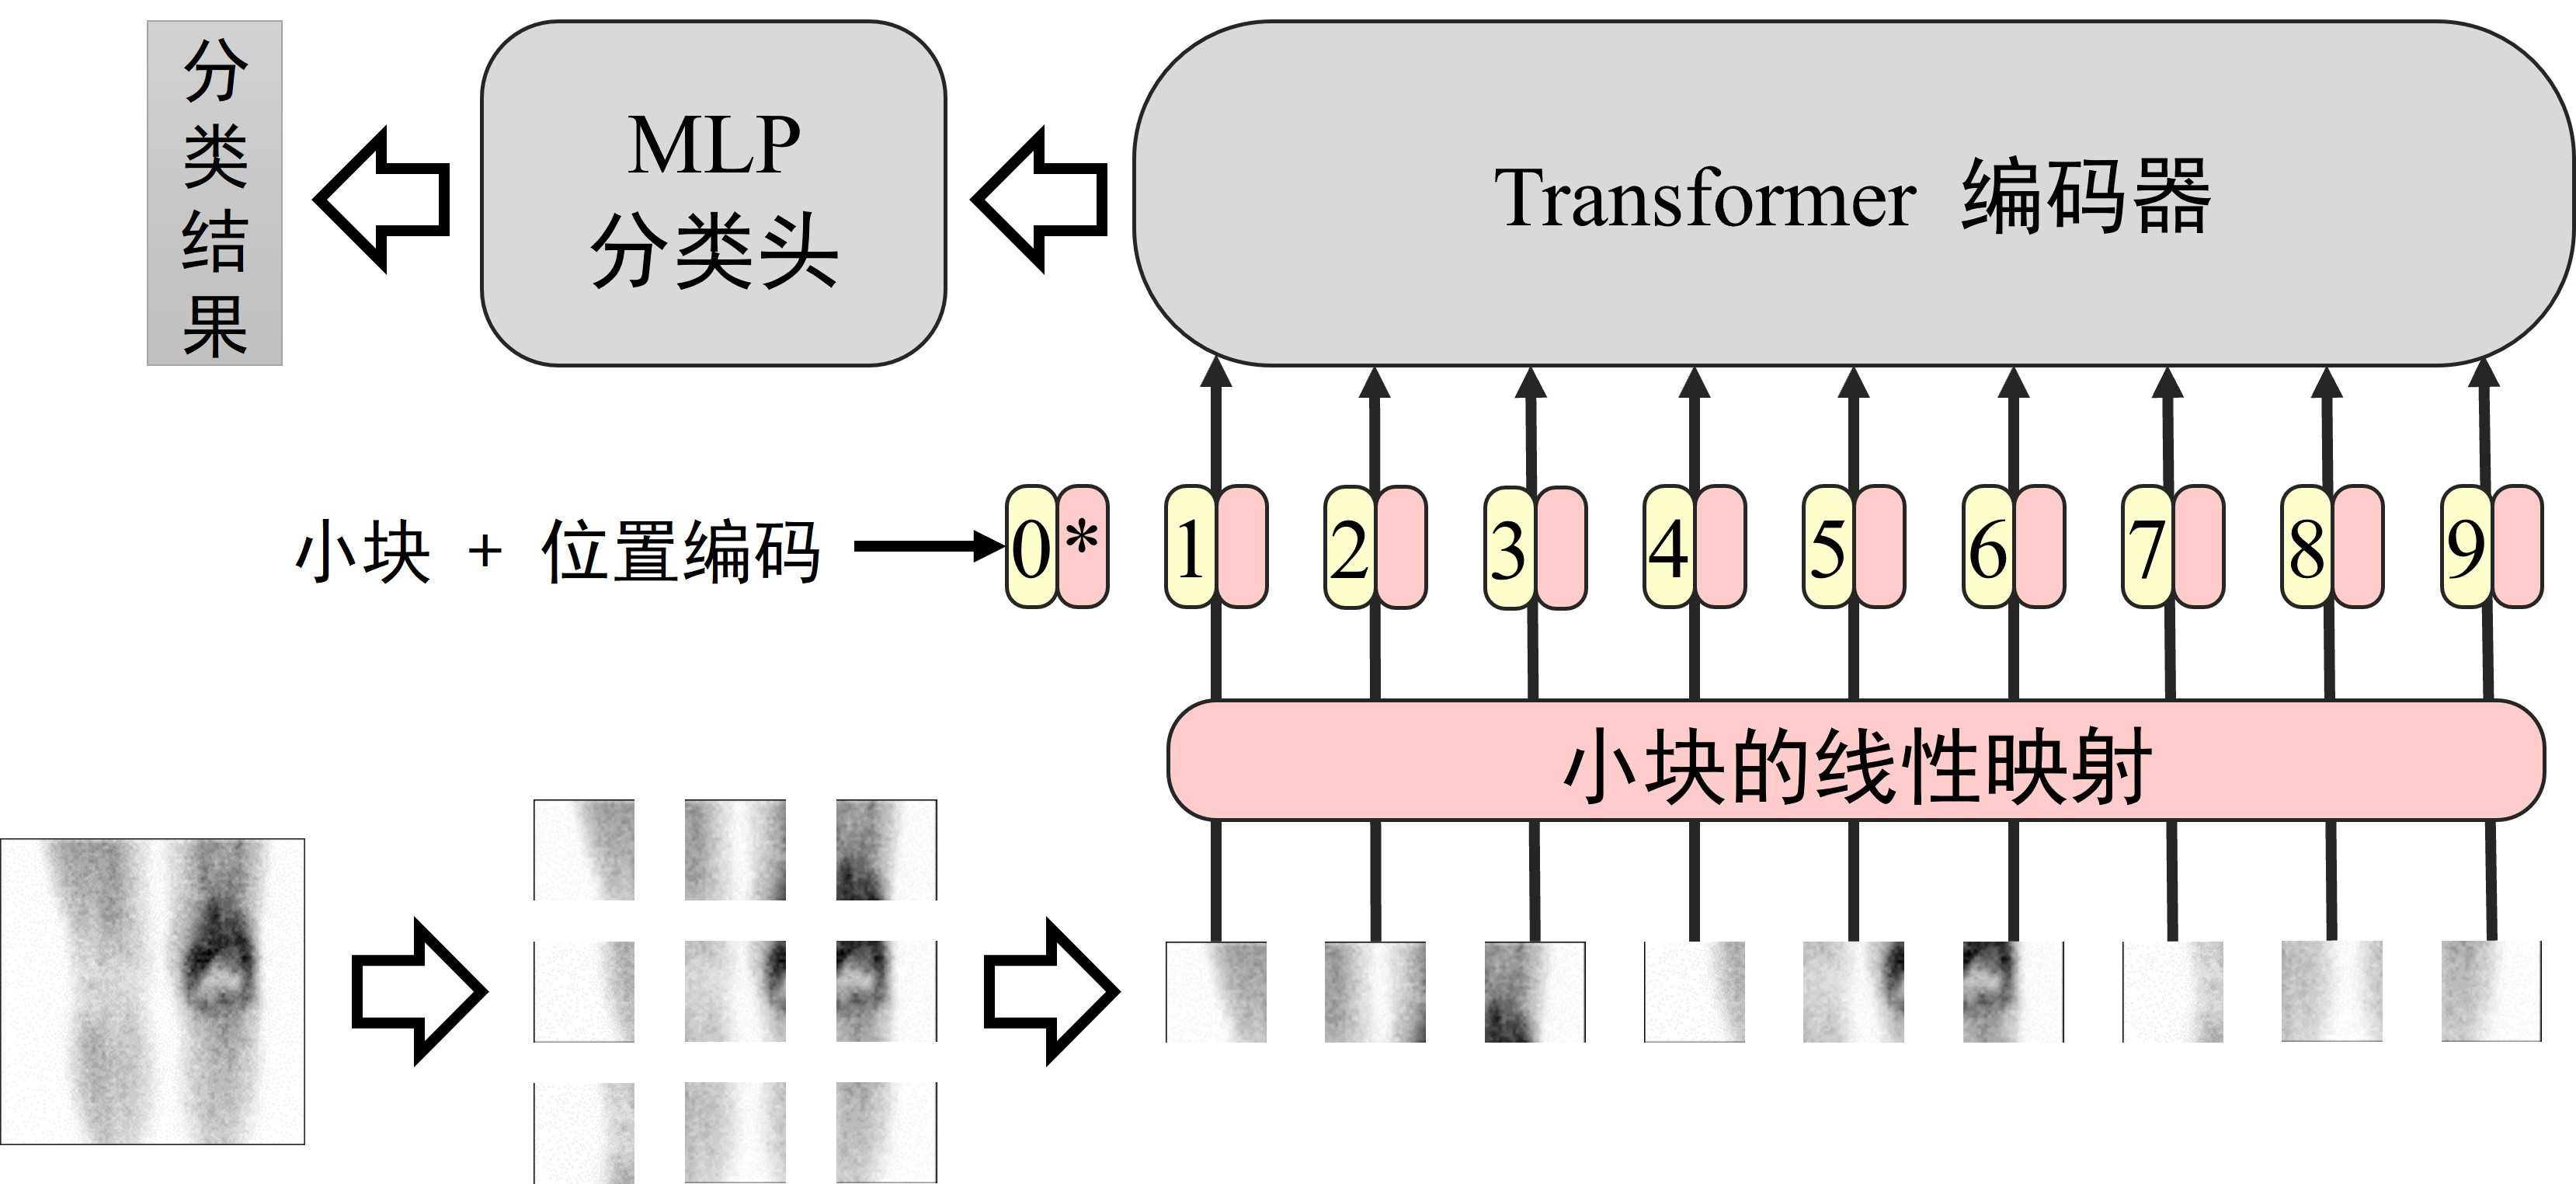
\includegraphics[width=\textwidth]{figures/chap02_vit.jpg}
  \bicaption{Vision Transformer示意图}{Schematic of Vision Transformer}
  \label{fig:chap02_vit}
\end{figure}

相比较于CNN,最初为自然语言处理任务设计的Transformer具有一些独特优势。即其自注意力机制在应用于图像时能够全面覆盖整个图像区域并聚焦于高度相关的特定区域。Dosovitskiy等人\cite{dosovitskiy2020image}于2020年的开创性研究引入了Vision Transformer(ViT),这是将Transformer模型成功应用于图像领域的首例,如图\ref{fig:chap02_vit}所示。ViT通过将图片分割成若干固定大小的小块(patches),并为每个小块赋予位置编码后构成序列输入到Transformer网络中。该模型通过捕捉图像中全局和局部的信息,来实现对图像特征的学习与分类。

Swin Transformer\cite{liu2021swin}(2021)是一种新型的Transformer,专为视觉任务设计。其创新之处在于引入了一个称为"shifted window"的机制,它允许跨越多尺度的特征交互。与传统Transformer相比,Swin Transformer通过此机制显著地减少了计算复杂性,使得在处理图像等高分辨率数据时更为高效。其工作原理是将图像分成多个小块,然后在这些小块中局部地应用自注意力机制,之后通过滑动(shift)这些小块的方式实现了全局信息的整合。

Transformer iN Transformer\cite{han2021transformer}(TNT,2021)是另一种创新Transformer架构,它在传统的自注意力机制中嵌入了一个自注意力机制。这个设计的关键是它内部具有两级Transformer结构:第一级抓取像素级的特征,而第二级聚焦于区域特征,从而对整个图像进行特征表示。这种内外Transformer的组合使得这个架构能够更有效地捕获图像内部的复杂结构。

综上所述,CNN和新兴的Transformer都是计算机视觉领域中的强大工具,它们在特征提取和模式识别方面展现出杰出的优势。对于CNN而言,其卷积层具有固定且较小的感受野,这使其能够有效地识别局部特征,如边缘、形状和纹理等,但可以通过多层堆叠以捕捉全局上下文信息。而Transformer通过自注意力机制可以捕捉到全局上下文信息,从而实现对整张图像的理解。然而,Transformer模型的训练需要依赖大量数据,而数据集小是医学影像领域普遍面临的问题。因此,CNN成为了更值得探索的方法。对于动态骨显像和PET/CT诊断分类任务而言,CNN可以有效地学习到病灶区域中局部关键性特征,例如生理摄取的形态和解剖结构的细节。然而,对于具有时序性特点的动态骨显像,由于CNN并非专门为处理序列数据而设计,其在这方面的能力是受限的。

\begin{figure}[htbp]
  \centering
  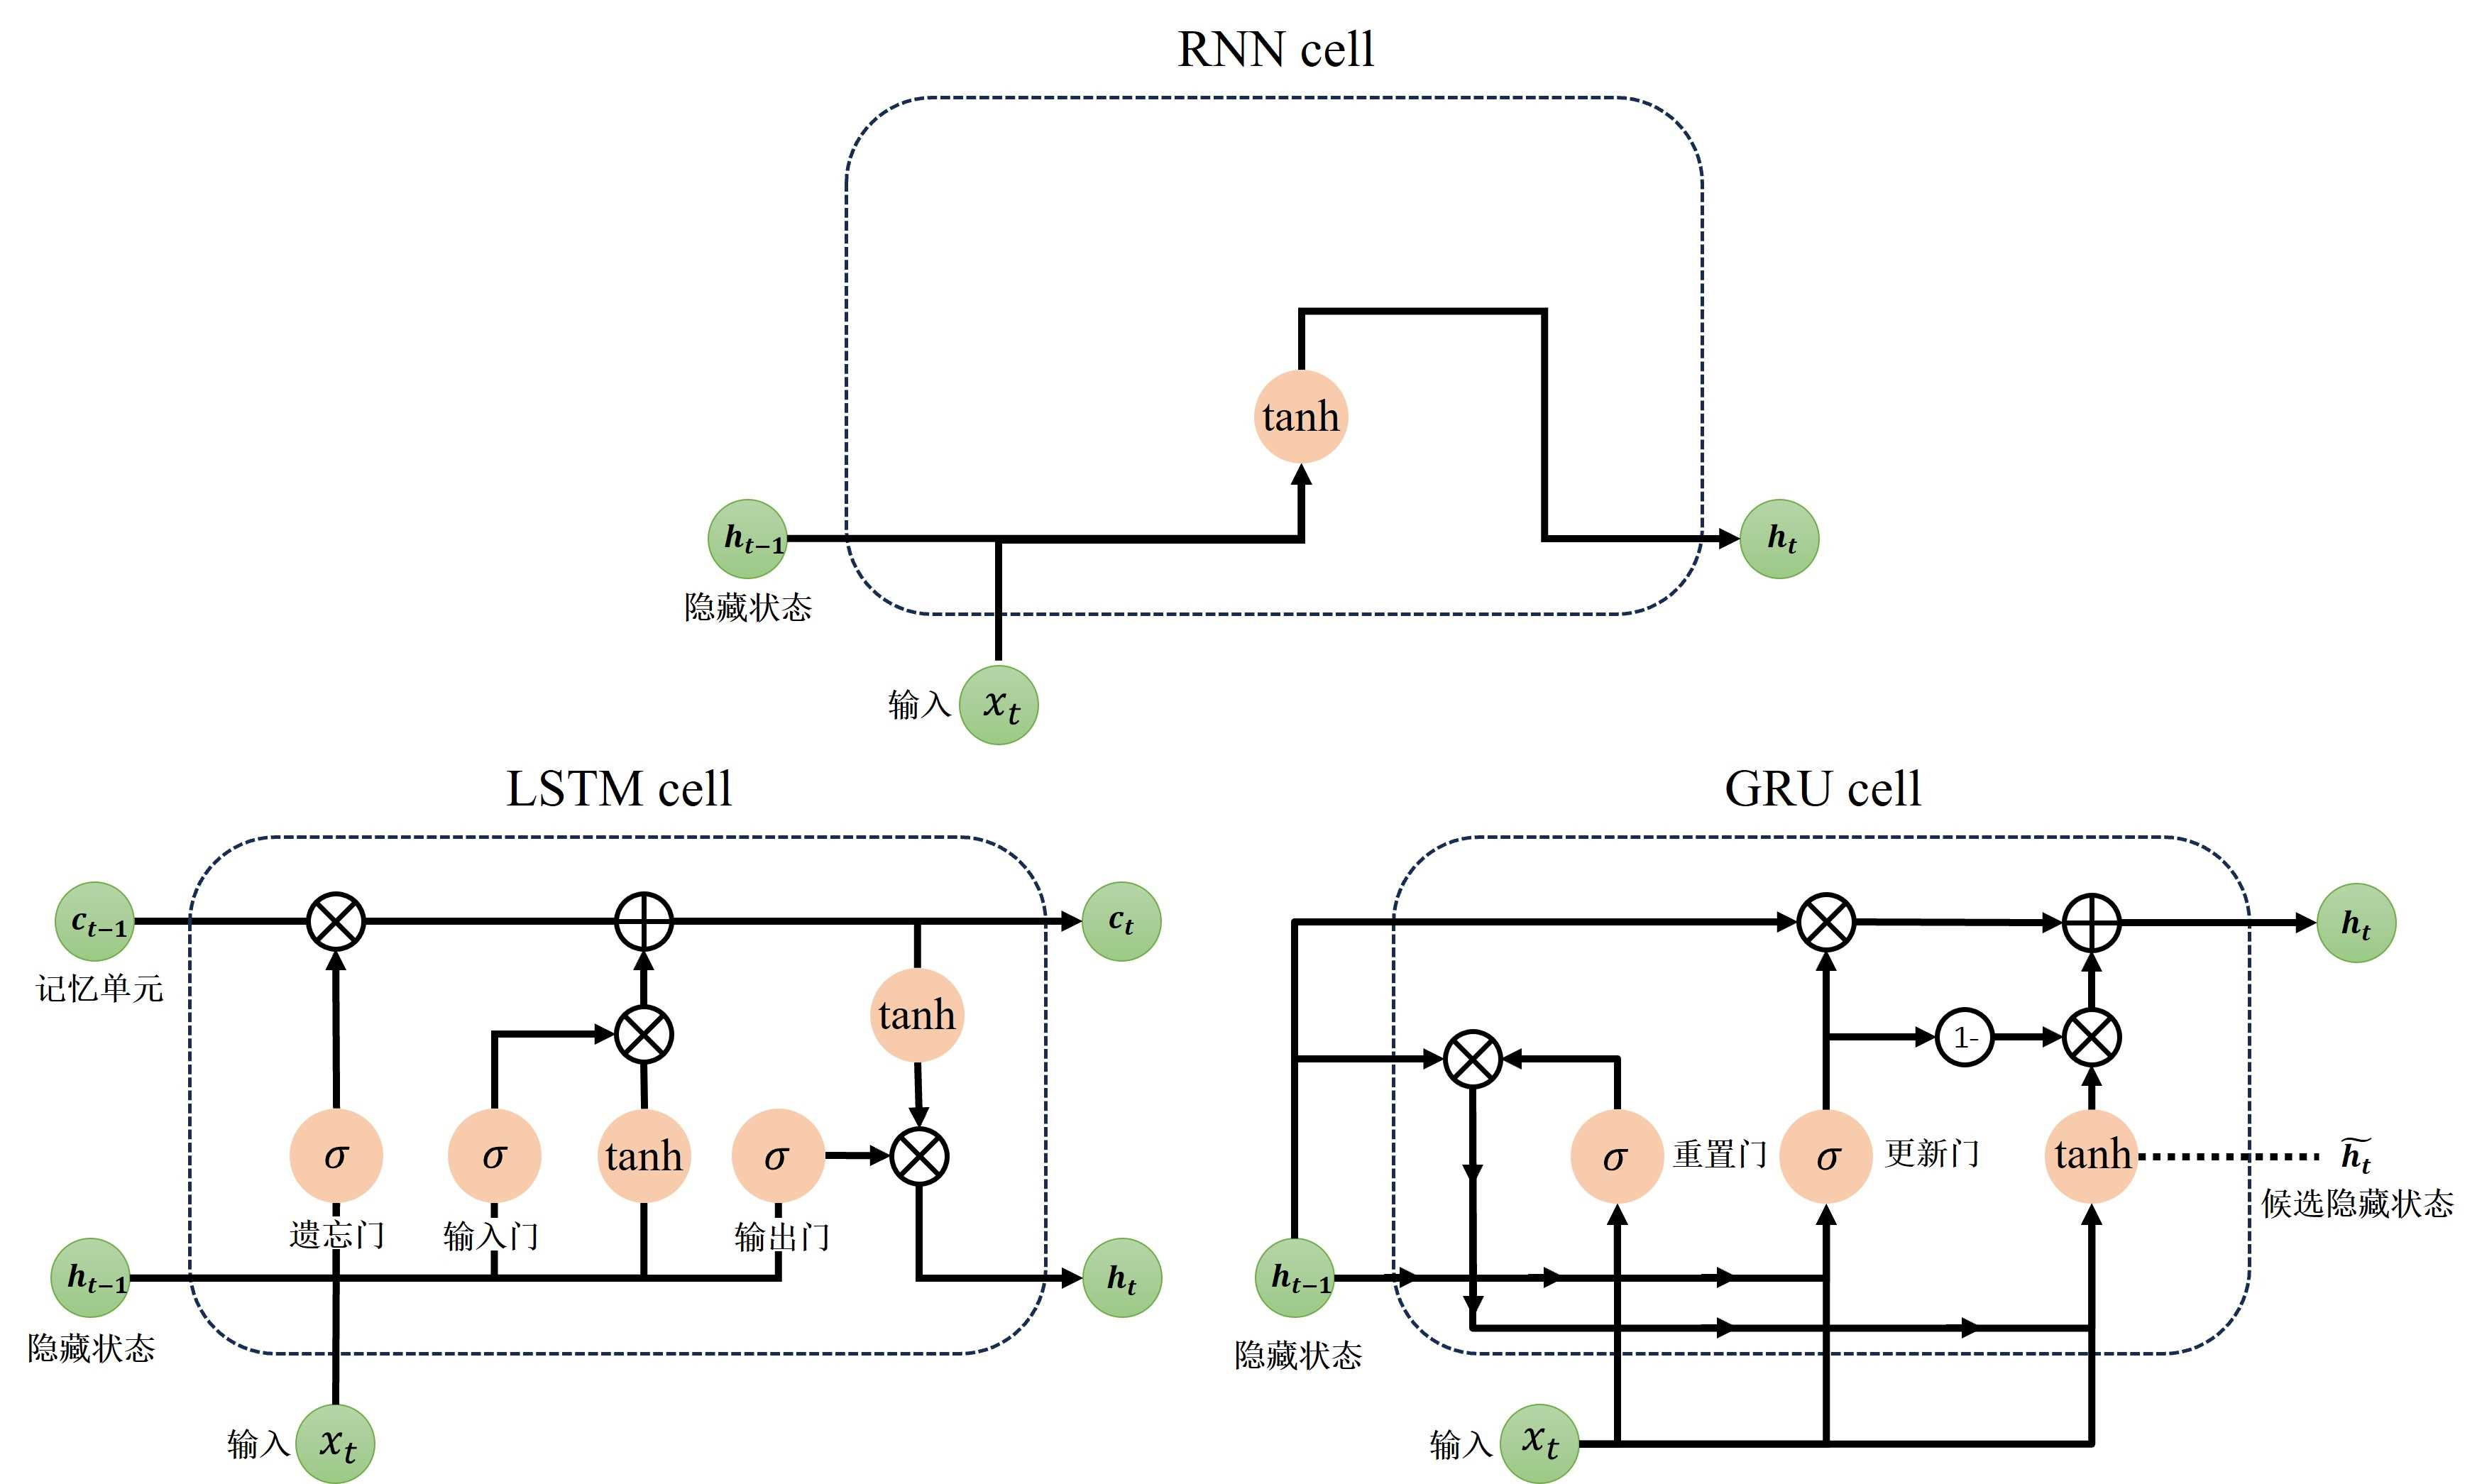
\includegraphics[width=\textwidth]{figures/chap02_rnn.jpg}
  \bicaption{循环神经网络示意图}{Schematic of the recurrent neural network}
  \label{fig:chap02_rnn}
\end{figure}

对比CNN,RNN作为深度学习方法之一,是一种专门用于处理序列数据的神经网络模型,非常适用于时间序列分析任务之中。RNN的主要原理在于它通过不断地更新隐藏状态(hidden state)去保存序列中每个时间点上一定的历史信息,并用于当前时间点的决策或下一时间点的预测,如图\ref{fig:chap02_rnn}。RNN的结构可以是序列到序列的形式,但当RNN应用于时间序列分析中的分类任务时,其结构可以变成序列到单一输出的形式。对于输入的序列数据\(X = \{x_1, \cdots, x_t, \cdots, x_T\}\)而言,在每个时间点\(t\)上,RNN通过以下公式更新隐藏状态\(h\):
\begin{equation}
  \begin{aligned}
    h_t & = \text{tanh}(W_{h}h_{t-1}+ W_{i}x_t) \\
    y^t & = \sigma_s(W_{h}h_{t-1})              \\
  \end{aligned}
\end{equation}
其中,tanh表示双曲正切函数,\(W_h\)和\(W_i\)分别表示上一隐藏状态到当前隐藏状态的权重和当前输入到当前隐藏状态的权重,\(\sigma_s\)表示Softmax函数,用于计算所属不同类别的概率分布,\(y^T\)表示RNN中的单一输出。

RNN在理论上可以捕捉长期依赖。但是在实际中,随着时间的增长,梯度消失或梯度爆炸的问题会出现,并且RNN学习和保留过去的历史信息的能力是有限的。为了解决RNN中存在的缺陷,研究人员提出了它的变体,长短时记忆网络(Long Short Term Memory, LSTM)\cite{memory2010long}和门控循环单元(Gated Recurrent Unit, GRU)\cite{chung2014empirical}。

LSTM\cite{memory2010long}(2010)相比较于RNN拥有一个更为复杂的结构,如图\ref{fig:chap02_rnn}所示。它在RNN的基础上添加了三个门控记忆单元(遗忘门、输入门和输出门)以及一个独立的记忆单元\(c_t\)来更新和输出隐藏状态。在长序列数据的处理中,LSTM展现出其强大的能力,通过动态地调节记忆单元,以实现时序信息的有效保留。在训练过程中,LSTM通过精确的门控机制,执行三项关键操作:首先,它利用遗忘门从单元状态中丢弃非核心信息;其次,它通过输入门引导新的信息加入单元状态;最终,它通过输出门精心挑选必要信息来构建输出。这一过程赋予了其在长时间跨度上维持和更新历史信息的能力,并捕捉到数据的深层依赖关系。由此机制,LSTM有效地克服了传统RNN面临的梯度消失与梯度爆炸问题。

GRU\cite{chung2014empirical}(2014)相比较于LSTM,简化内部繁琐的门控机制,如图\ref{fig:chap02_rnn}所示。它在LSTM的基础上将隐含状态与记忆单元合并为一个统一的隐藏状态,并通过两种门控单元(更新门与重置门)来控制信息流动。更新门的作用是调节前序隐藏状态对当前隐藏状态的影响程度,允许模型在必要时保存跨越较长时间区间的信息。而重置门则决定在当前隐藏状态的更新过程中,前序隐藏状态的参与程度,这样使得模型可以有选择性地忘记或保留过往信息。GRU通过更加灵活和精简的门控策略来维持长期的状态信息,并同时捕获短期的上下文特征,这一策略在许多实验中被验证能够有效预防梯度消失的问题。

Yiugit等人\cite{yiugit2021simple}于2021年提出了两种简单且有效的GRU变体:GRU1和GRU2。通过一种基于经验的方法,这些学者试图确定一组能够提高GRU准确度或降低损失的系数\(\epsilon,\alpha\)。其中,\(\epsilon\)确定门控循环单元的作用力度,\(\alpha\)确定门控当前单元门的作用力度。相比较于GRU,GRU1增加了当前单元的作用,而GRU2减少了循环单元的作用。值得说明的是,对标准GRU算法进行这样微小且简便的调整能够显著提升其性能。

综上所述,RNN及其变体为处理序列数据提供了富有弹性的学习架构。RNN以其简单的循环连接结构,去捕获时序信息,但仍存在梯度消失或爆炸的问题。LSTM和GRU则引入门控机制,有效地保存长期依赖关系,优化了信息的存储与过滤,降低了梯度消失和爆炸的风险。对于动态骨显像中的假体关节感染诊断任务而言,不仅需要关注每张图像中的病灶摄取形态特征,还需要抓取跟时序相关的生理代谢差异变化特征,RNN和CNN的有效结合将适用于该任务的模型设计,同样也是图像序列分类任务的重点研究方向之一。

\subsection{医学影像分类算法}

计算机辅助诊断(computer aided diagnosis, CAD)是通过计算机对病患的医学影像,如PET、CT、MRI等,进行分析并辅助医生完成相应疾病的诊断流程。计算机依靠逐渐流行的深度学习技术,可以自动地从目标数据中学习获得更深层次的特征,并且排除人为因素的影响,实现全自动化的辅助诊断。基于医学影像的分类诊断是计算机辅助诊断的重要研究方向之一。对于不同的医学影像而言,由于其本身的成像技术不同,从而拥有不同的特性和成像效果,这也是科研人员不可忽视的研究基础之一。根据医学影像的特点,有效设计合适的图像处理算法和模型结构有助于提升分类诊断任务的质量。

Cheng等人\cite{cheng2017classification}(2017)提出了一个级联的三维CNN用于脑部PET影像的分类诊断。该方法首先划分整个PET脑影像为数个三维的局部子区域。接着,利用一个三维卷积网络来提取每个子区域中更深层次的鉴别特征。最后,应用一个高级别的三维卷积网络来融合各个子区域特征,实现对阿尔茨海默症患者与健康对照组的有效区分。
Liu等人\cite{liu2018classification}(2018)在阿尔茨海默病的诊断领域,采用了创新性的方法,将CNN与RNN相结合。把三维PET影像分解为二维切片序列,通过二维卷积网络学习切片内部的特征和RNN掌握切片间的序列特征,来展现对阿尔茨海默病的高效分类性能。
Khagi等人\cite{khagi2020cnn}(2020)提出了一种用于脑部MRI和PET影像进行分类诊断的三维卷积架构divNet。它可以有效区分阿尔茨海默症、轻度认知障碍和正常,用于协助临床医生进行初步快速检测来确定患者的病情。
Lee等研究者\cite{lee2021performance}(2021)对PET影像进行了深入探究,评估了Inception3D、ResNet3D以及VGG3D三种深度学习架构在阿尔茨海默病诊断中的性能表现。结果显示,这些模型在诊断任务中平均准确率高达95\%。在进一步的外部验证中,VGG3D具有最佳的泛化能力。
Liu等人\cite{liu2022diagnosis}(2022)提出一种创新性多尺度CNN来用于脑部MRI影像中的阿尔茨海默病的诊断。该网络通过引入通道注意机制,改善通道间的相互依赖关系,自适应地调整通道维度上的特征,来增强它的特征表达能力。大量实验证明,通过将MRI划分为白质(white matter) 和灰质(gray matter)来进行训练,该网络以更少的参数和更低的计算复杂度获得了最优异的性能。
Takahashi等人\cite{takahashi2022deep}(2022)探索了一种创新的图像预处理方式,即采用了多角度的最大强度投影(Maximum Intensity Projection,MIP),如图\ref{fig:chap02_mip}所示。他们将MIP预处理后的三维PET影像输入至深度学习模型中进行训练,使其能够识别乳腺癌的标志性特征。在随后的性能评估中,该模型展现出了超越没有经验的放射科医生的诊断能力,与三名专业放射科医生相当的诊断能力。

\begin{figure}[htbp]
  \centering
  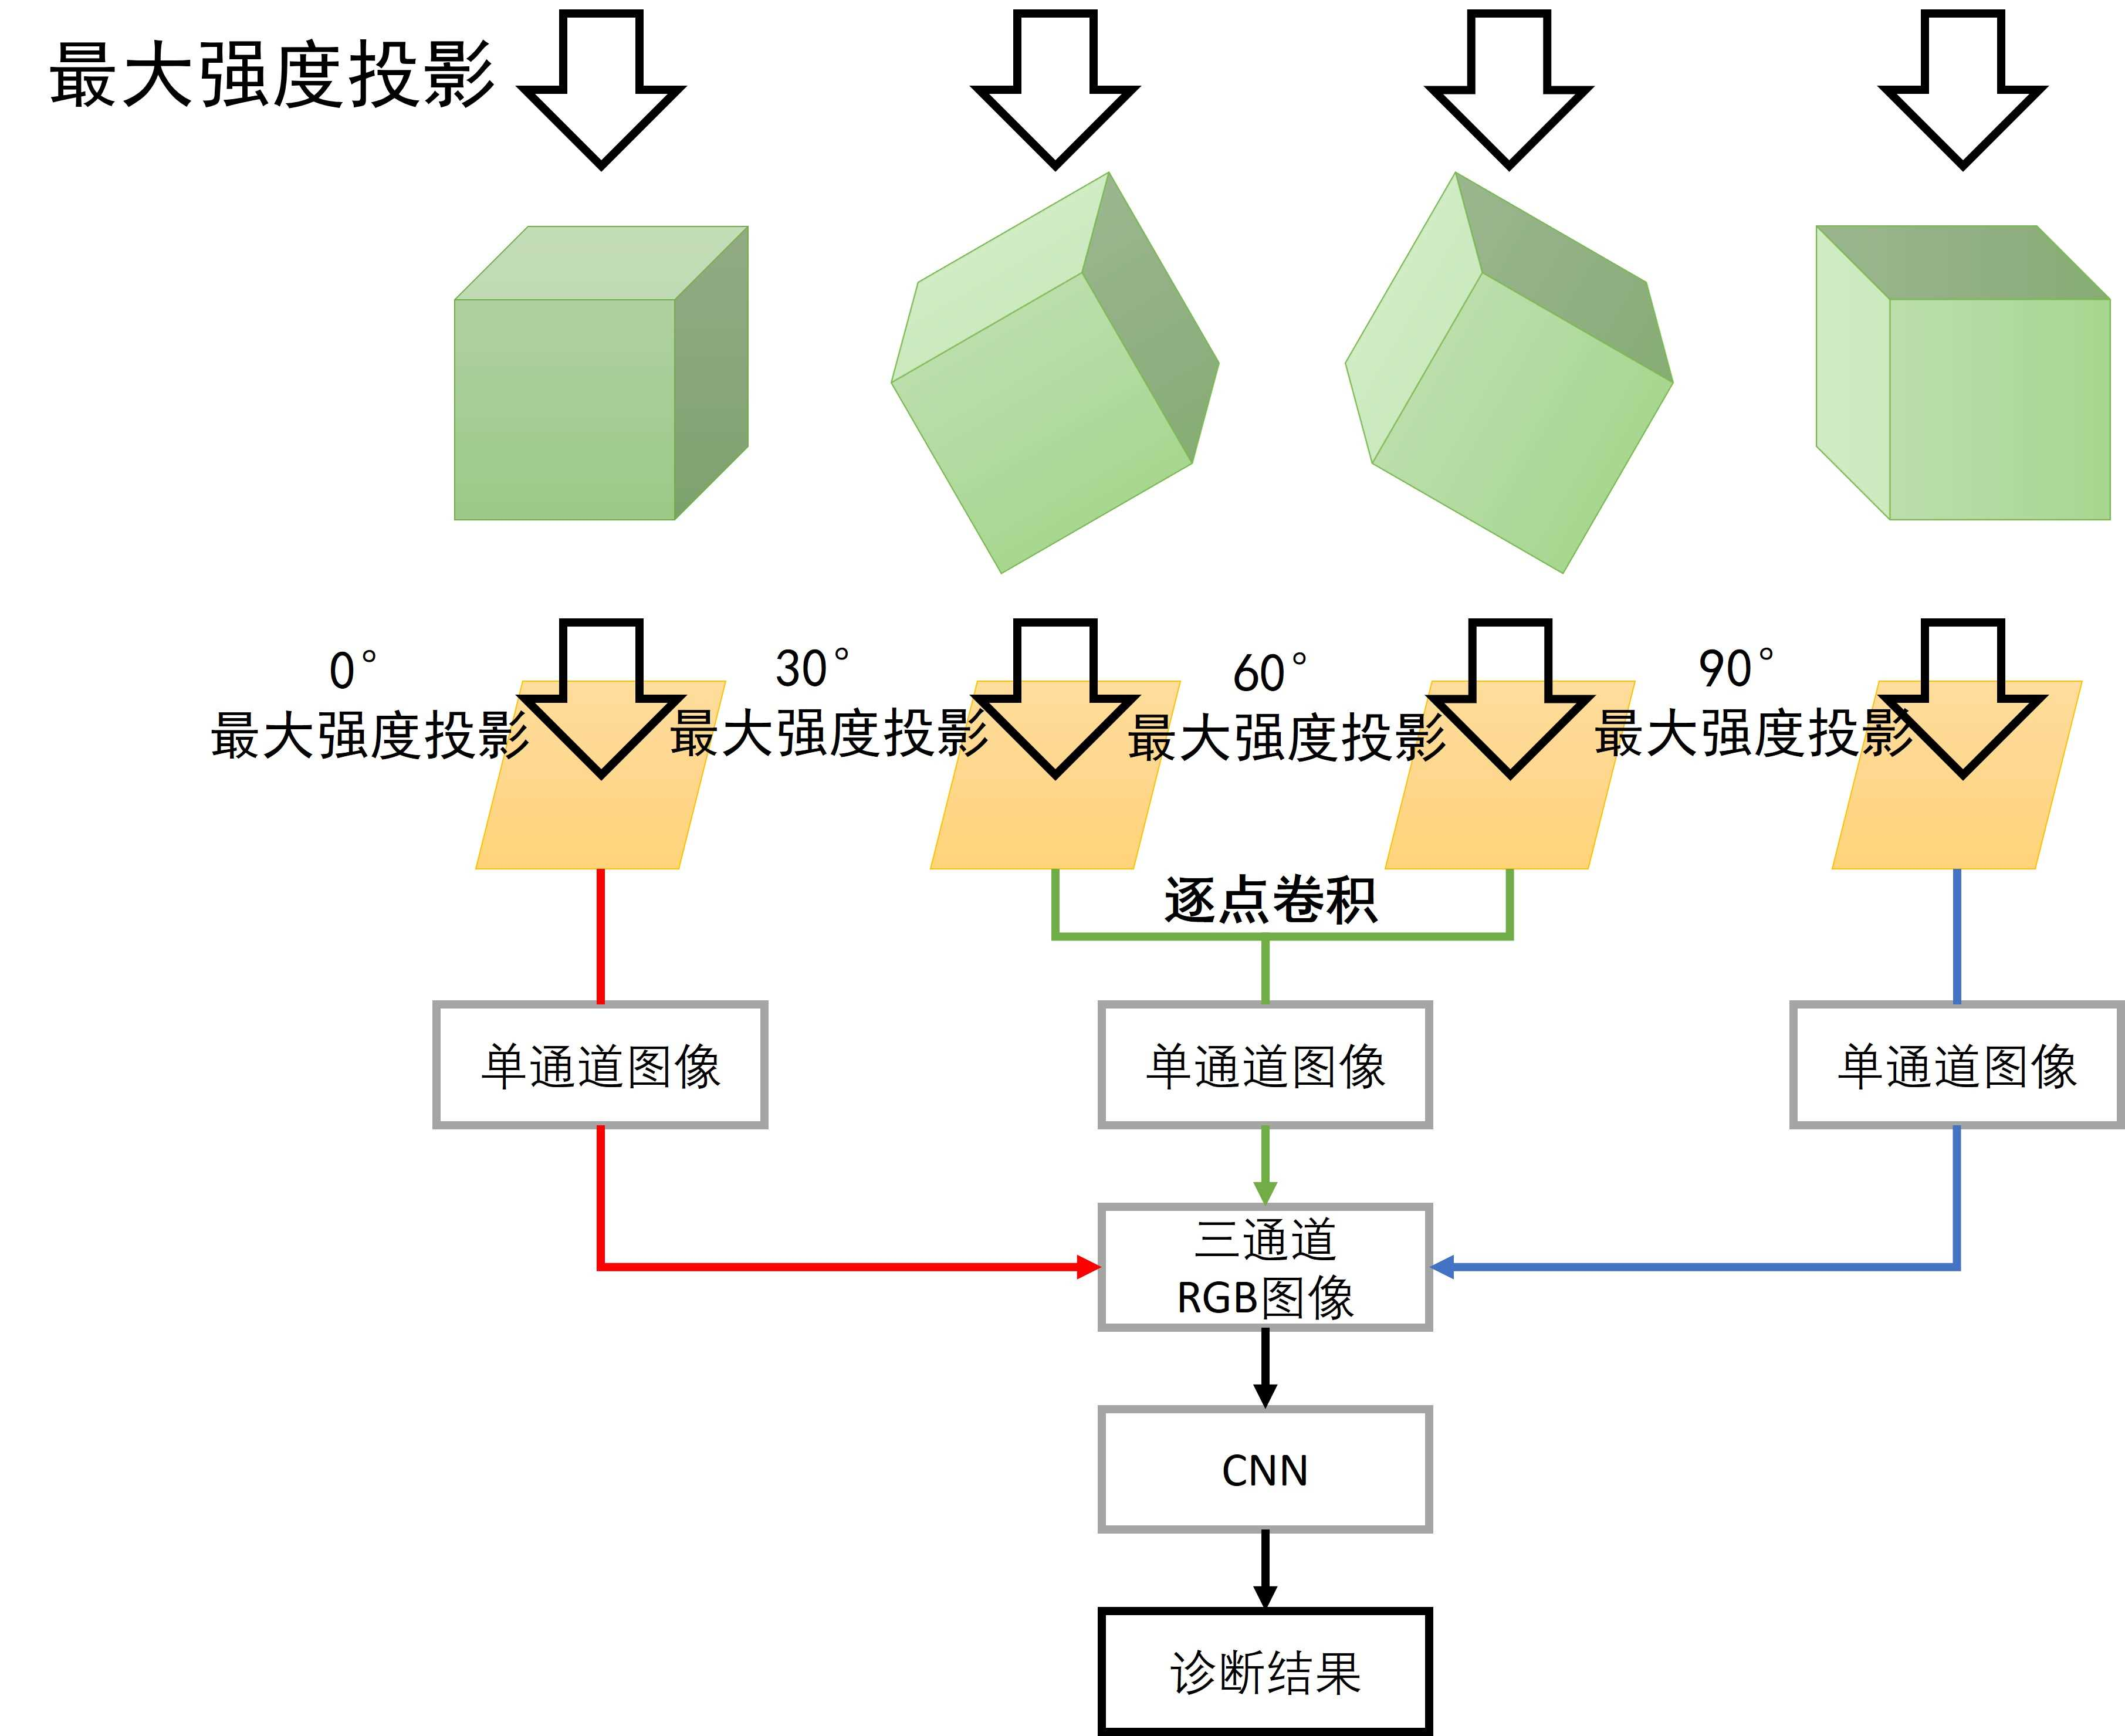
\includegraphics[width=0.8\textwidth]{figures/chap02_mip.jpg}
  \bicaption{四个角度最大强度投影图像作为输入进行预测的示意图}{Schematic of four angular maximum intensity projection images as input for prediction}
  \label{fig:chap02_mip}
\end{figure}

综上所述,对于动态骨显像中假体关节感染任务,以上研究存在一些可借鉴之处。例如,将时序性图像的固有三维性质,直接采用三维CNN进行特征提取似乎是一种直观的策略。然而,传统的CNN在捕捉长期时序依赖方面存在局限性。由此,结合使用CNN和RNN,以便在时间序列的内部和之间提取综合特征,对于该特定医学任务来说可能更加精准和适宜。同时,也应该重视任务的特定难点,比如无关区域干扰和生理状态下高摄取区域可能对分类精度造成的负面影响。鉴于此,研究并设计针对动态骨显像的数据预处理方法,去有效减少负面影响,进一步优化深度学习模型的性能,是提高诊断精准度的关键。

在PET/CT影像中的骨折相关感染任务中,考虑到PET/CT为三维影像数据,直接采用三维CNN是一个不错的选项,以便充分利用体积数据的空间信息。同时,考虑到计算复杂度和数据维度的挑战,采用MIP对数据进行降维处理也是一个有效的替代方案。此外,针对PET/CT影像的特定情况,如多病灶的存在和相对较小的病灶区域在整体影像中难以突显导致传统的深度学习模型可能无法有效集中于关键的病灶区域的问题,需要特别关注。因此,开展针对PET/CT影像的专门预处理方法研究和引入检测算法定位病灶区域,并对其进行截取或突出处理,可以在不损失重要信息的前提下减少背景噪声的干扰,进而提高深度学习模型在骨折相关感染检测任务中的准确性和效率。

\section{图像检测}

检测任务通常指输入数据中一个或多个目标物体的识别与空间定位过程。图像检测,在计算机视觉领域内,是解决“识别图像中存在的目标对象以及这些目标对象的准确位置”的关键性问题。该任务适用于众多领域,例如安防监控、自动驾驶、医学影像分析等等。

在医学影像分析中,检测任务特别强调了对疾病标志物的精准定位与识别,如肿瘤、异常组织等,从而为临床诊断提供关键的影像学依据。随着深度学习技术的发展,检测任务通常是要求模型通过边界框来准确发现并定位目标对象。在深度学习与医学影像分析相结合的背景下,检测任务有时会通过像素级分类,即图像分割,来增强目标的定位精度。无论是哪种定位方式,这都需要检测模型具有理解和区分图像中各种复杂特征的能力,以便实现对不同的目标对象的准确识别和区分。

在骨折相关感染的诊断流程中,医生通常集中审视病灶区域在生理代谢方面展现的摄取形态,因为与感染相关的特征通常紧密聚焦于这些区域。对此,探讨检测任务中的神经网络架构显得尤为重要。本节将概述有关于此方面的研究现状,并分析这些架构应用于PET/CT影像上进行骨折相关感染病灶区域检测的可行性。

\subsection{图像检测算法}

在执行检测任务的深度学习模型分类上,一般可划分为目标分割模型与目标检测模型两大类。目标分割模型,以U-Net\cite{ronneberger2015u}为代表,旨在实现对图像中每个像素所属类别的识别,从而获取精确的目标形状与位置。这类模型在医学影像中尤为重要,因为它允许细致划分病灶区域,为后续的量化分析提供了基础。相对地,目标检测模型,如区域卷积神经网络(Region with CNN features,R-CNN)\cite{girshick2014rich}和YOLO(You Only Look Once)\cite{redmon2016you},往往通过预测边界框来定位目标对象,提供了一种相对较快且效率更高的检测方法,尽管其定位的精细程度相对较低。无论是哪种类型的模型,其设计和优化都在不断地促进医学影像分析与计算机视觉领域的研究进展,继而改善临床诊断与治疗的质量。

\begin{figure}[htbp]
  \centering
  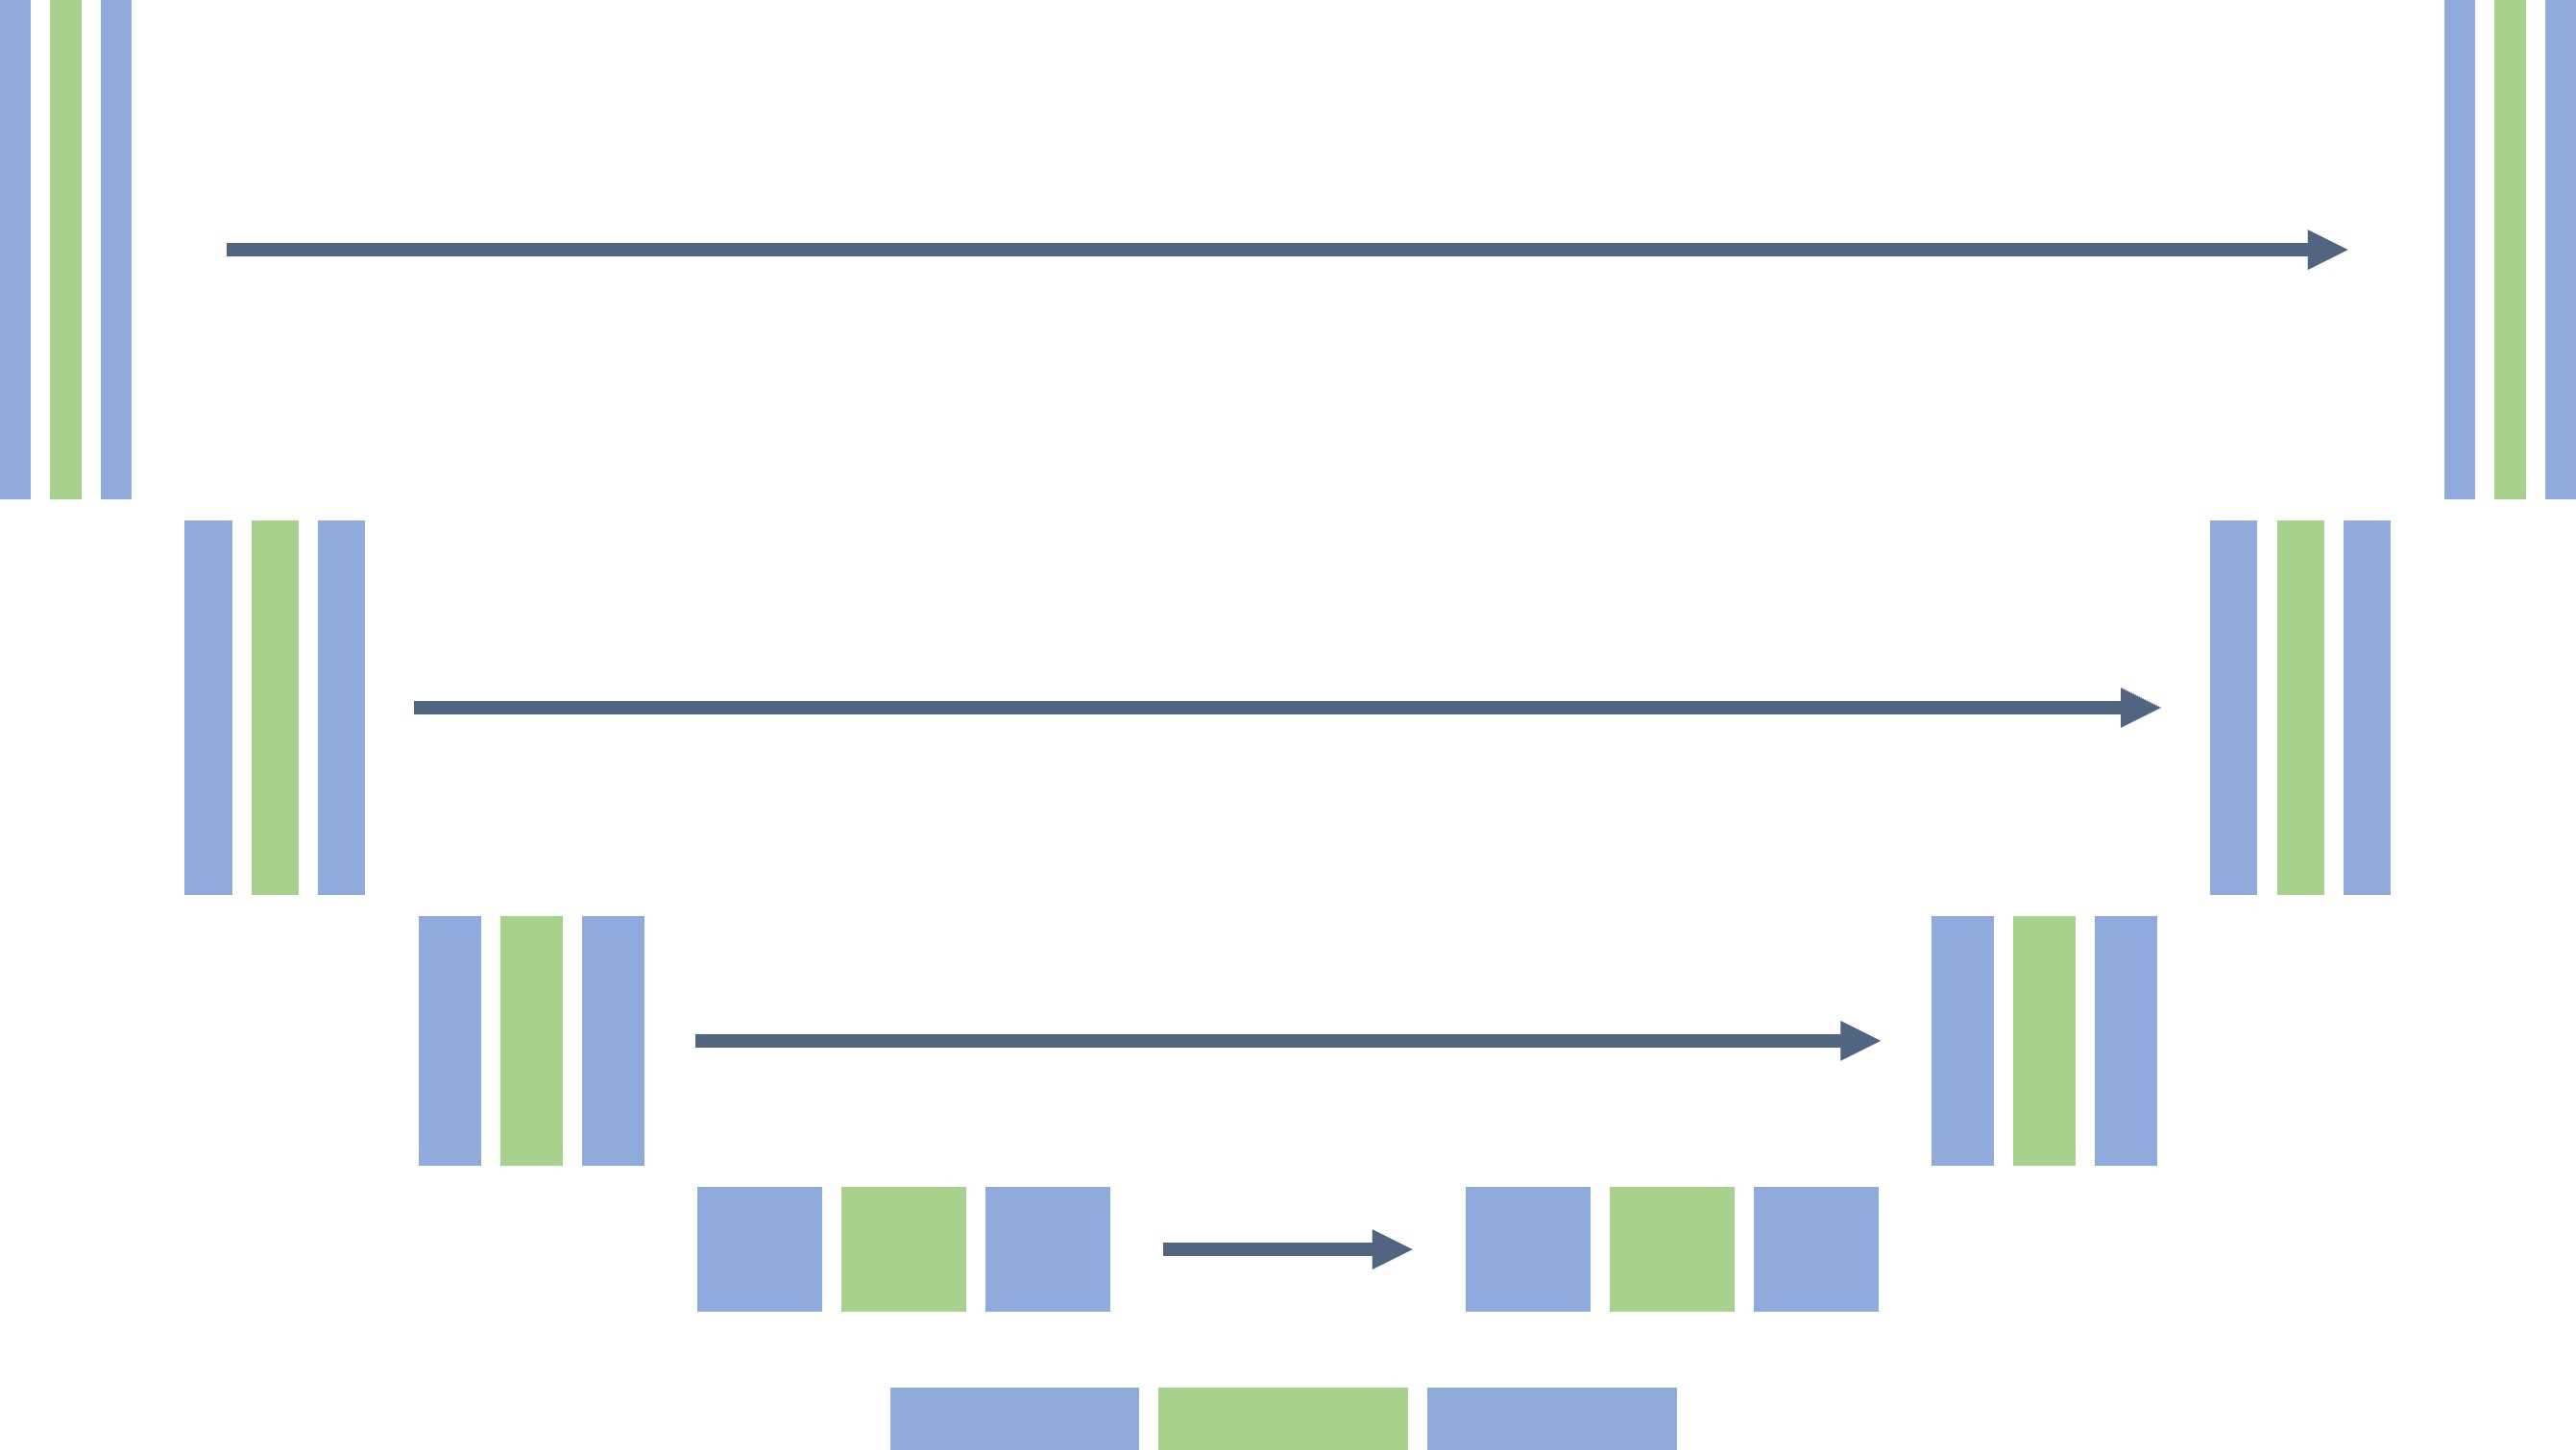
\includegraphics[width=\textwidth]{figures/chap02_unet.jpg}
  \bicaption{U-Net整体结构示意图}{Schematic of the overall structure of U-Net}
  \label{fig:chap02_unet}
\end{figure}

在目标分割模型中,U-Net\cite{ronneberger2015u}(2015)的提出开辟了医学影像分割任务的新纪元。它是一种专为医学图像分割设计的深度学习模型结构,摒弃了之前模型对大量数据依赖的限制,在较少标注样本的情况下仍能实现高效能的模型训练。在结构上,如图\ref{fig:chap02_unet}所示,整体呈现为一种“U”字形的对称结构,包括下采样(收缩路径)和上采样(扩展路径)两个部分,能够捕获上下文中多尺度的语义信息。下采样阶段逐步提取特征并降低数据维度大小,而上采样阶段逐步恢复数据维度大小并进行特征解码。同时,通过跳跃连接将下采样阶段的语义信息与上采样阶段的位置信息相结合,以增强特征并实现精确的定位。

U-Net++\cite{zhou2018unet++}(2018)是U-Net\cite{ronneberger2015u}的嵌套版本,强化了特征学习能力,增强了模型对复杂医学影像的分割准确度。主要的创新点包括跳跃连接的重新设计和深度监督。在跳跃连接方面,U-Net++添加了密集的跳跃路径,允许模型结合来自不同阶段的特征,从而提升了捕捉细节、特征融合与学习的能力。在深度监督方面,U-Net++为了充分利用多尺度的语义信息,在每一层的嵌套路径上,都可以输出一个分割图结果。通过所有的分割图结果一起联合优化,有效地强化了模型对不同尺度特征的学习。

Attention U-Net\cite{oktay2018attention}(2018)是一种集成了注意力机制的改进型U-Net\cite{ronneberger2015u}。这种机制可以使得模型更加关注于影像中的关键部分,从而提高特征的区分力和医学影像分割的准确性。其核心的创新点在于跳跃连接中加入了注意力门控模块,以便过滤和引导传统的跳跃连接特征,使得网络能够集中学习更有价值的信息。

U-Net 3+\cite{huang2020unet}(2020)是在U-Net的基础上发展出来的一种医学影像分割模型。该模型通过引入全尺度跳跃连接和深度监督机制,增强了对多尺度特征的融合,并提高了模型的学习能力。全尺度跳跃连接保证了各个解码阶段中全尺度特征的充分利用,而深度监督机制在各个解码阶段直接引入了额外的监督,确保了模型在多层结构上的有效特征学习和提取。

TransU-Net\cite{chen2021transunet}(2021)是一种结合了卷积强大的局部特征提取能力和Transformer的全局自注意力机制的新型网络架构。它先使用卷积提取空间特征,再利用Transformer编码器以捕获长距离上下文关系,最后通过解码器来输出精确的分割结果。这种混合架构使得TransU-Net在分割精度上超越了传统的CNN网络。

综上,U-Net及其变体具有强大的特征学习能力,在医学影像处理中得到了广泛的应用。每个变体都是为了解决特定问题而设计,比如改进特征的捕获能力、更精确地分割图像中的特定部分等。随着深度学习技术的进步,将会有更多的U-Net变体被提出来解决更复杂的医学影像分割任务。在PET/CT中,用于识别骨折相关感染病灶的任务面临的挑战在于感染区域的形态分布呈现多样性,包括但不限于点状、簇状或弥散性分布。这种分布的复杂多样性导致利用像素级定位进行精确标注和检测变得较为困难。因此,本研究的重点在于目标检测模型。

在目标检测模型中,深度学习方法主要分为两大类:二阶段检测器和一阶段检测器。

\begin{figure}[htbp]
  \centering
  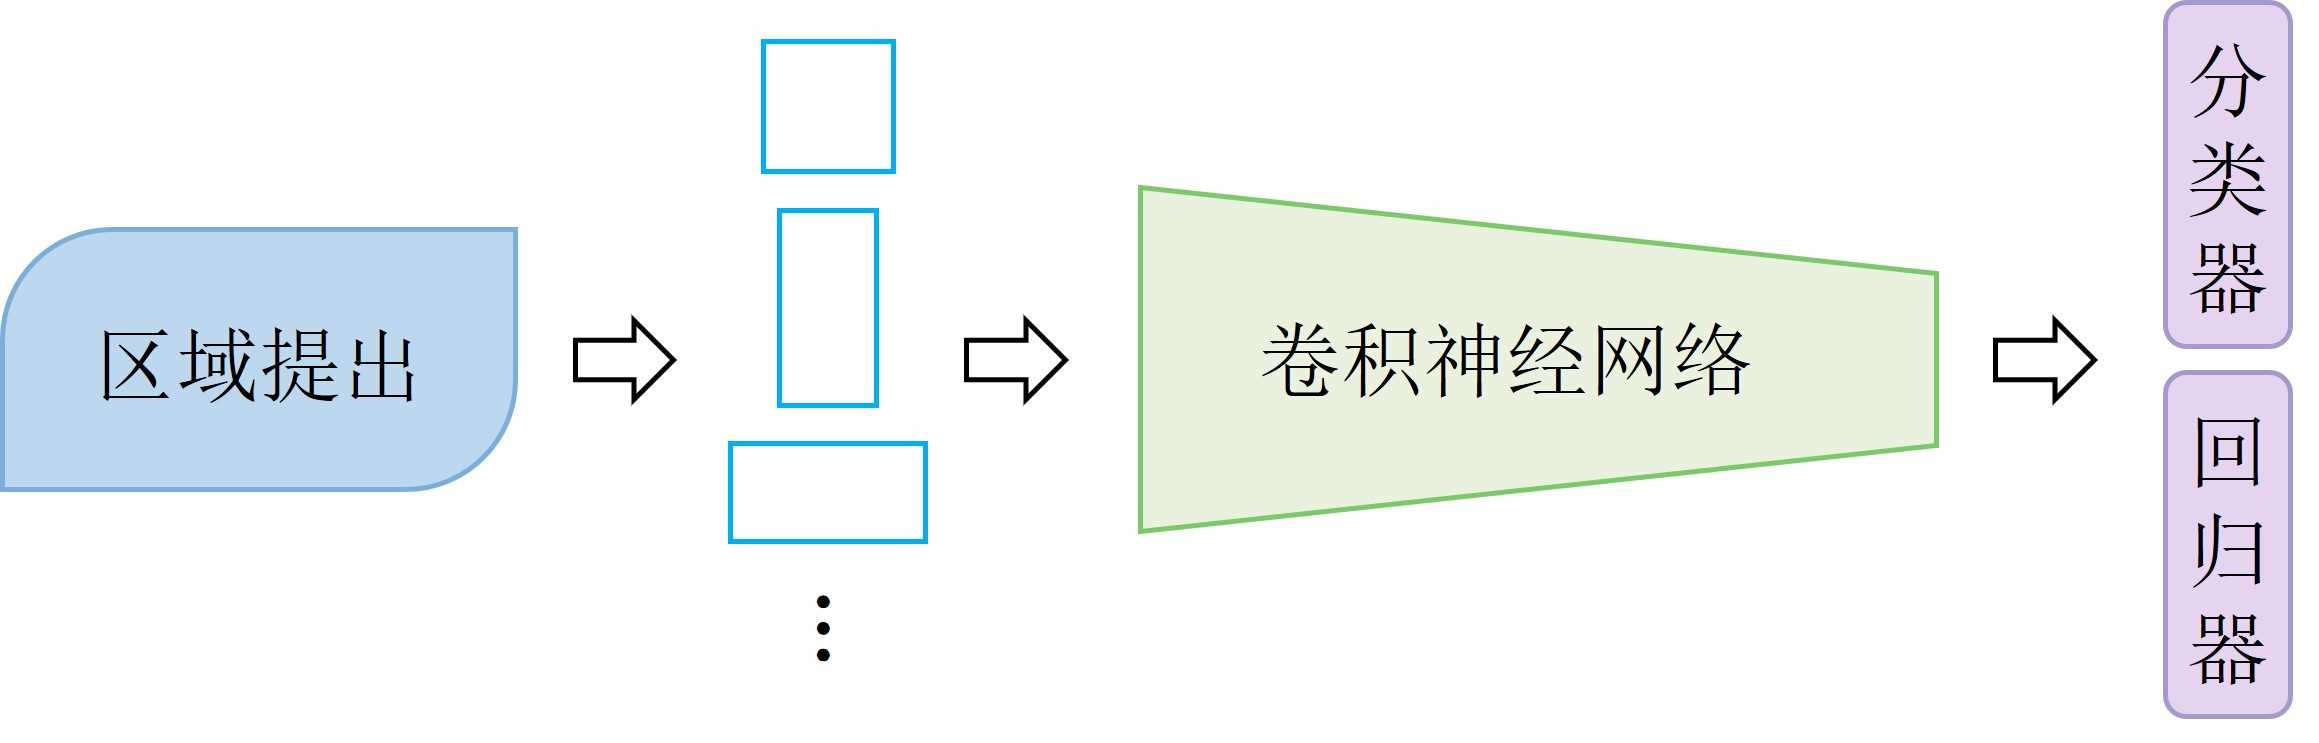
\includegraphics[width=0.8\textwidth]{figures/chap02_rcnn.jpg}
  \bicaption{R-CNN整体结构示意图}{Schematic of the overall structure of R-CNN}
  \label{fig:chap02_rcnn}
\end{figure}

二阶段检测器的工作流程分为两个阶段:1.生成目标的候选区域;2. 提取这些区域的特征进行分类和边界框的精调。在具有里程碑式的二阶段检测器中,R-CNN\cite{girshick2014rich}(2014)是第一个开创性的二阶段检测器,整体结构如图\ref{fig:chap02_rcnn}所示。在R-CNN模型中,首先由选择性搜索(Selective Search)算法依据图像特征如颜色、纹理、形状等,负责挑选出潜在含有目标对象的候选区域。随后,对这些区域进行标准化预处理,并通过预训练的CNN提取特征。最终,由分类器对特征区域进行分类,并通过边界框回归器精确调整目标对象的位置,以提升目标检测的准确性。虽然R-CNN在其推出时对目标检测领域产生了巨大的影响,但它也存在一些缺点,例如速度慢、训练需要对不同部分分阶段进行,存储需求高。为了克服这些缺陷,后续基于R-CNN的改进模型,如Fast R-CNN\cite{girshick2015fast}和Faster R-CNN\cite{ren2015faster},被提出。

Fast R-CNN\cite{girshick2015fast}(2015)对整个目标检测流程进行了端到端的优化,使得模型可以同时执行目标分类任务和目标定位任务,从而提高了训练速度、检测效率和检测精度。该方法的核心创新点有两个:一是共享了CNN提取的整个图像的特征,采用了感兴趣区域池化技术,在该特征图上对多个大小不同候选区域映射为固定大小的特征。二是将目标分类和边界框回归进行结合,并提出了多任务损失函数用来同时优化分类和回归任务。

Faster R-CNN\cite{ren2015faster}(2015)在Fast R-CNN的基础上创新地引入了区域提议网络(Region Proposal Network,RPN),它能够替代掉选择性搜索算法,并且学习如何快速且高质量地生成候选区域。RPN与Fast R-CNN的结构无缝地整合在一起,进一步提升了目标检测的效率与准确性。这不仅实现了整个过程端到端的训练和较之前模型的显著加速,还成为目标检测领域的又一里程碑。

一阶段检测器,相比较于二阶段检测器,跳过了候选区域的生成阶段,直接对图像中的目标进行位置和类别的预测。它们通常使用全卷积网络来分析图像,使得在推理过程中能够获得更快的速度。

\begin{figure}[htbp]
  \centering
  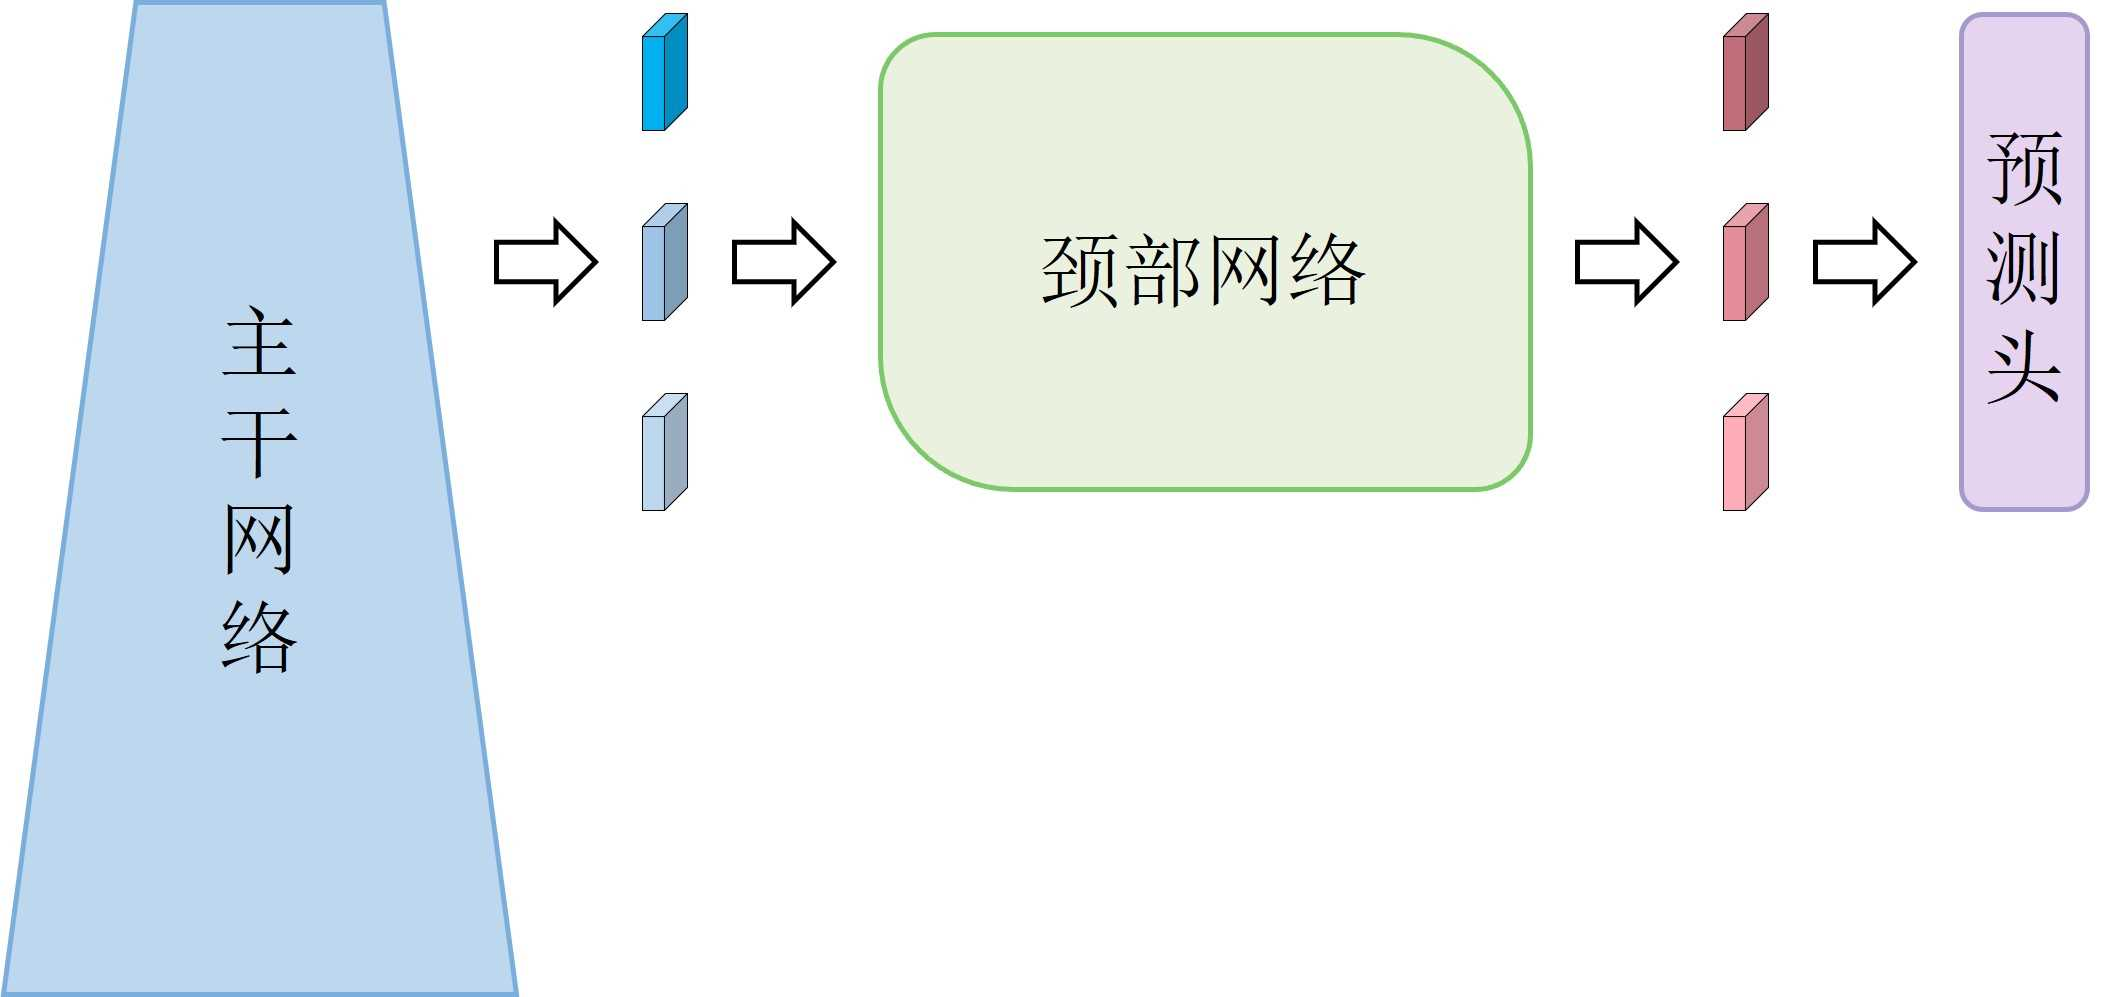
\includegraphics[width=0.8\textwidth]{figures/chap02_yolo.jpg}
  \bicaption{YOLO整体结构示意图}{Schematic of the overall structure of YOLO}
  \label{fig:chap02_yolo}
\end{figure}

YOLO\cite{redmon2016you}(2016)是一阶段检测器中非常流行且影响深远的一种端到端的目标检测器。其核心思想是把目标检测任务转换为一个回归问题来解决。YOLO采用一个单一的神经网络结构去全图预测,如图\ref{fig:chap02_yolo},其结构可大致分为三个部分:用于特征提取的主干网络,用于特征融合的颈部网络和用于预测的头部网络。YOLO将输入图像划分为多个网格,每个网络预测多个目标的边界框和类别以及一个置信度。置信度反映了边界框包含目标的可能性。由于YOLO的设计简单直观和检测速度高效,它在现实世界中应用广泛,并且不断地在各个版本中得到改进,并确保在速度和准确度间取得更好的平衡。

YOLOv2\cite{redmon2017yolo9000}(2017)是YOLO\cite{redmon2016you}的改进模型。它在保持高速检测的特点上,通过引入批标准化、使用更高分辨率输入、增加锚框来改善边界框预测、更换主干网络以及利用多尺度训练来提高对不同尺寸目标的检测能力,从而大幅提升了检测精确度,尤其在小目标的检测上。

YOLOv3\cite{redmon2018yolov3}(2018)进一步提高了检测性能。它引入了多尺度预测来加强对小目标的识别能力,还通过加深主干网络来增加网络的特征学习能力并保持了合理的运算效率。它还采用了逻辑回归进行类别的预测,并优化了描框的机制以更好地适应不同形状的目标。整体上,YOLOv3在速度与准确度之间获得了更优的平衡。

YOLOv4\cite{bochkovskiy2020yolov4}(2020)是目标检测领域中又一重要进展,其在YOLOv3\cite{redmon2018yolov3}的基础上,综合了多项新技术来进一步提升检测准确率并且保证高速处理。该版本采用了跨阶段部分(Cross Stage Partial)\cite{wang2020cspnet}结构应用于主干网络中,引入了Mish\cite{misra2019mish}激活函数,使用了路径聚合网络(PANet)\cite{liu2018path}和空间金字塔池化(SPP)\cite{he2015spatial},增强了网络的特征提取和特征融合能力,同时包含了多种检测技术,如自适应锚框计算等等。

YOLOv5\cite{jocher2020yolov5}(2020)是YOLO系列的又一迭代,而其自身就迭代了多个版本。它采用了模块化的设计,可以选择不同大小的模型,更易于使用。YOLOv5包含了自动学习的锚框尺寸、多尺度训练、权重剪枝优化等技术,使模型既可以在资源有限的设备上运行,也能在需要高精确度的场合中保持较高性能。

YOLOX\cite{ge2021yolox}(2021)是一个新兴的目标检测架构,它在YOLOv3的基础上做了优化和改进,目标是在性能和灵活性之间取得更好的平衡。YOLOX的主要特点是它放弃了原有的锚框机制,采用了无锚框的设计,这使得网络在训练时对各种大小的目标有更好的适应能力。除此之外,YOLOX采用了解耦的头部设计,在分类和回归两个不同的任务上分开进行预测。

综上所述,一阶段目标检测器得益于算法和计算能力的提升,在目标检测任务中表现出色。它们在处理速度上显著优于二阶段检测器,满足实时处理的需求。速度的提升并未以牺牲准确率为代价,经过精心的网络设计和训练,一阶段检测器在不断地缩小与二阶段检测器的精度差距,甚至超越了它们。因此,在PET/CT的病灶检测任务中,面对感染区域的复杂多样性,选择一阶段检测器提供了一个既快速又准确的检测策略。

\subsection{医学影像检测算法}

在医学影像领域中,基于深度学习的检测算法已经逐步应用于现代的诊断过程之中。随着医学影像技术的发展,如MRI、CT和PET等成像技术不断进步,产生了大量的高维度和高质量的医学影像数据。这些影像含有丰富的生物医学信息,对于疾病的早期发现、诊断和治疗监测提供了重要依据。为高效、准确地解读这些复杂的数据,基于深度学习的医学影像检测算法被广泛研究和部署。

Tang等人\cite{tang2018automated}(2018)的研究提出了一种创新的架构,专门用于CT中的肺结节检测。该研究构建了一个受U-Net启发并结合3D Faster R-CNN的检测模型用于提出肺结节的候选框,还设计了一个三维卷积神经网络去降低假阳性。
Li等人\cite{li2019mvp}(2019)在神经网络设计中巧妙地融合了人类的专业知识,提出了一种具有位置感知注意力机制的多视图特征金字塔网络。该网络专门针对常见的病变检测任务,在CT的三种不同视角下,有效地利用三维医学影像信息。
Al-masni等人\cite{al2020two}(2020)提出了一种全自动、两阶段的集成深度学习框架,旨在高效地检测脑微出血。第一阶段中,YOLO被采用来识别潜在的脑微出血候选区域;随后,在第二阶段,引入了一个三维卷积网络来减少检测结果中的假阳性。
Mei等人\cite{mei2021yolo}(2021)在YOLOv4的基础上,结合各种现有的技术,如深度过参数化卷积层、卷积注意力模块和焦点损失函数,并进行了冗余的通道修剪,提出了一种更高效且实用的肺结节检测器YOLO-lung。
Lee等人\cite{lee2021dual}(2021)提出了一个创新的头颈部肿瘤分割框架。此框架采用了U形结构,设计了一种具有双分支和交叉注意力模块的编码器以及一个解码器。此外,模型集成的应用进一步强化了框架的分割性能。
Wang等人\cite{wang2022maff}(2022)提出了一种创新的多尺度自适应注意力特征融合网络,专注于PET/CT中的胰腺病变检测。该网络的核心创新体现在基于多模态的双特征提取网络和特征融合网络,以获得丰富的多尺度特征的同时让语义信息更加集中,提高了检测的精确性。
Huang等人\cite{huang2022isa}(2022)利用深度学习技术,提出了一种融合了PET高敏感度和CT精细解剖信息的创新性目标分割方法,如图\ref{fig:chap02_isanet}所示。此方法在编码阶段采用双模态的输入策略,并在解码阶段对不同模态信息进行特征融合,最大化地挖掘PET和CT各自的优势。这一方法可以有效地提高肿瘤分割性能。

\begin{figure}[htbp]
  \centering
  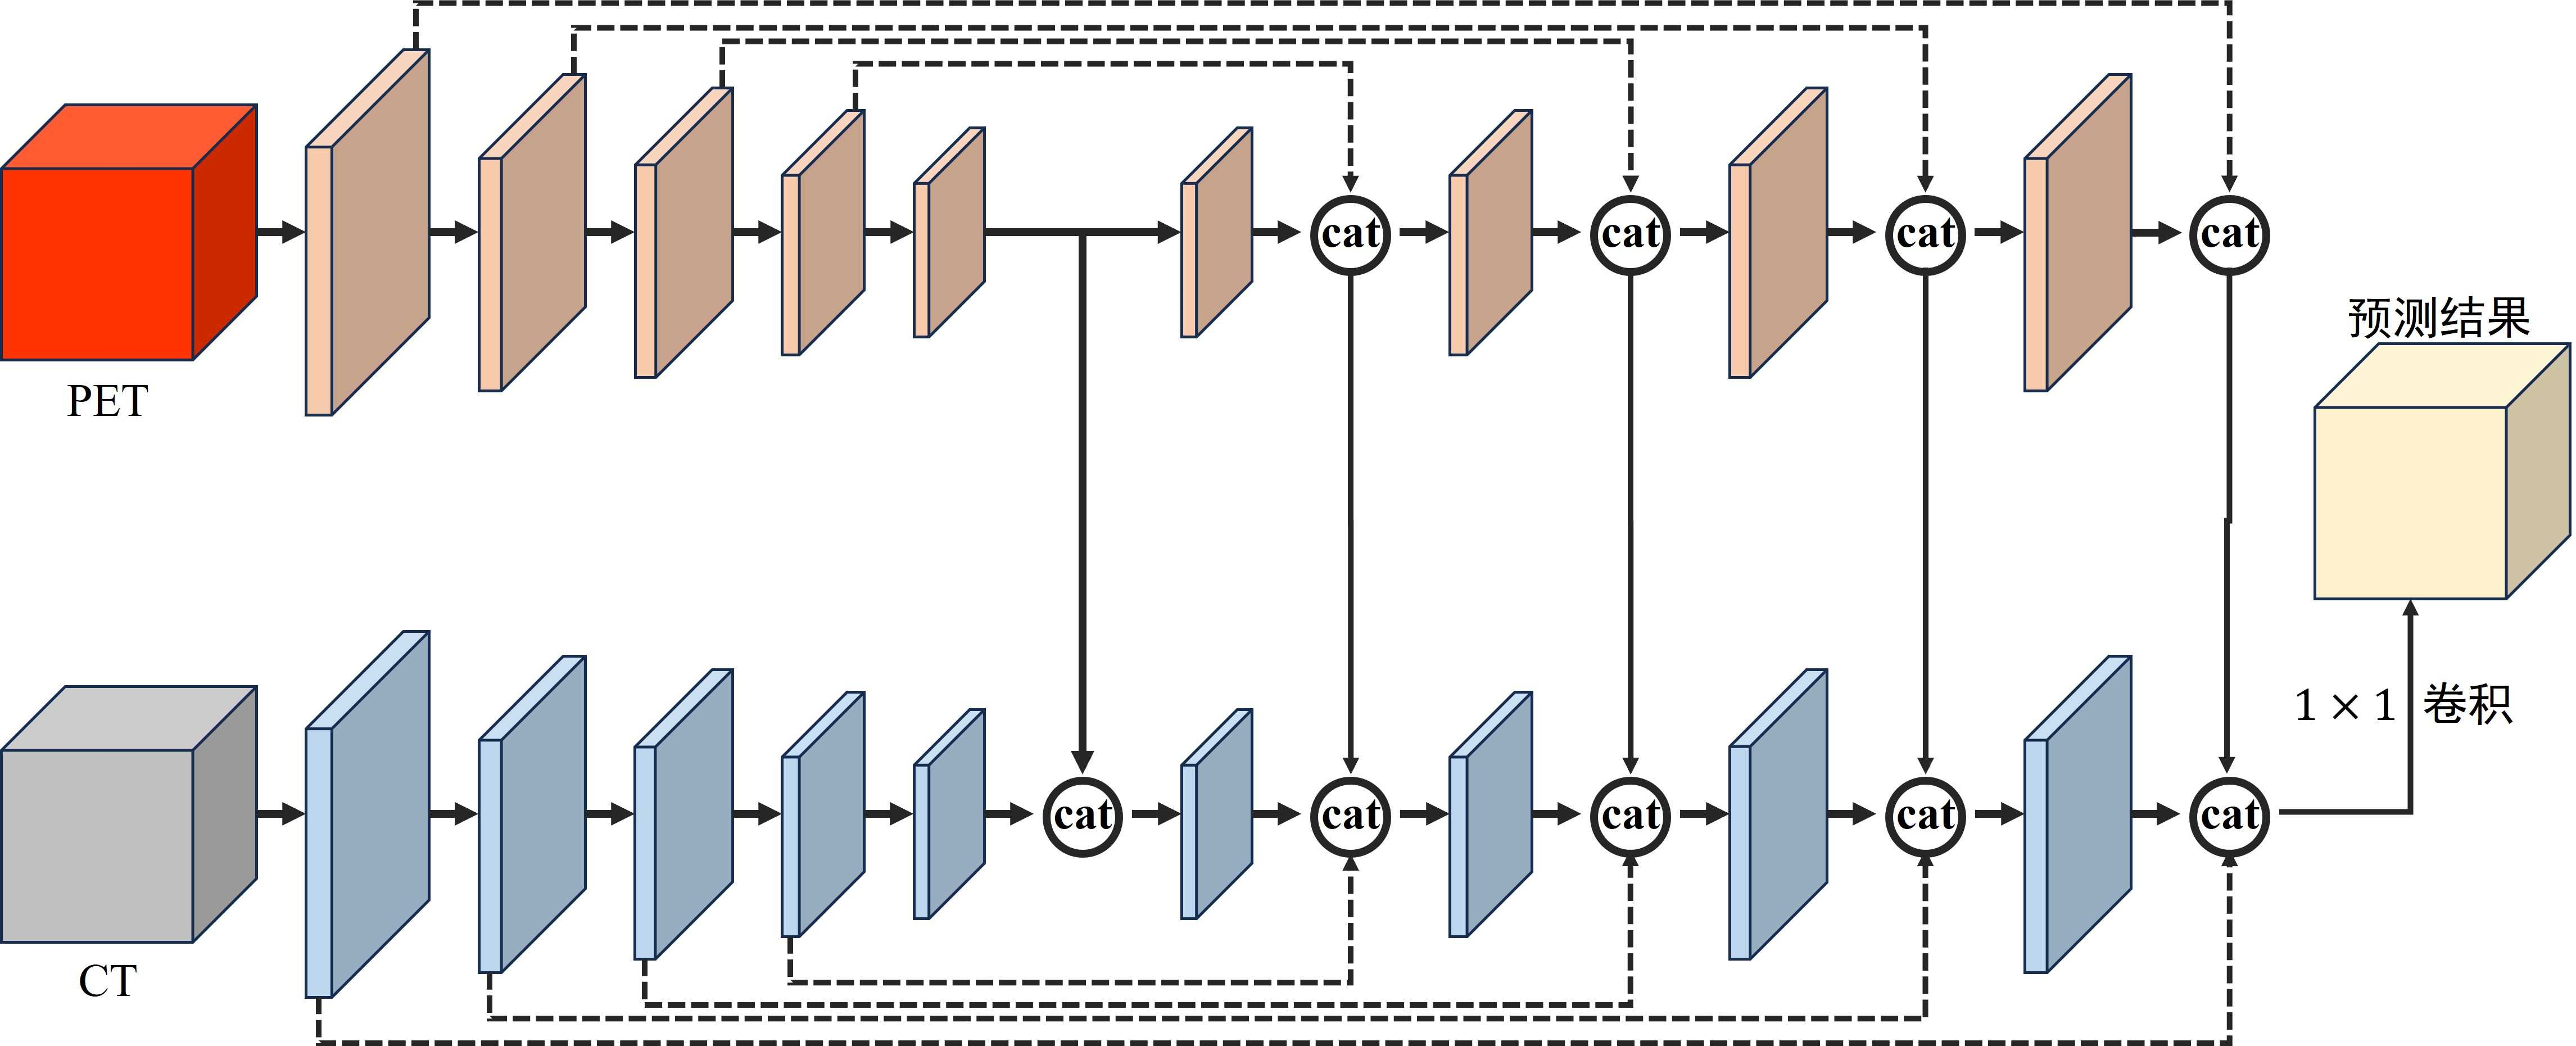
\includegraphics[width=\textwidth]{figures/chap02_isanet.jpg}
  \bicaption{融合PET和CT的目标分割方法}{Object segmentation method by fusing PET and CT}
  \label{fig:chap02_isanet}
\end{figure}

通过上述研究,可以明确认识到在PET/CT中定位骨折相关感染的任务需要充分利用PET与CT两种不同模态提供的信息。整合和发挥两者的独特优势至关重要。因此,探讨一个双分支网络架构是一个非常值得考虑的方向。同时,还需面对PET/CT中高摄取区域所带来的干扰问题,并采用创新性的实用方法予以解决。借鉴以往研究中有效的技术方案,并结合本研究任务的具体特性,提高定位准确性是本研究努力的核心目标。

\section{本章小结}

本章首先回顾了分类任务的核心流程及其发展变化。继而,着重解析了CNN、ViT和RNN的基础理论和关键特性,并针对本研究所涉及的分类任务,探讨了这些模型的适用性。同时,本章亦涵盖了近期医学影像领域分类研究的进展,并详细审视了这些进展对于本项研究所具有的借鉴意义。此外,特别强调了深度学习领域中检测算法的研究,梳理与总结了当下普遍应用的网络架构的发展脉络,在医学影像检测领域的最新研究动态,并从中归纳出适于本研究检测任务的方法,为后面的研究提供了坚实的基础。
% !Mode:: "TeX:UTF-8"
\chapter{基于\texorpdfstring{\(^{99m}\)}{99m}Tc-MDP动态骨显像的假体关节感染辅助诊断框架}

上一章介绍了用于分类和检测任务中的人工智能方法,以及它们在医学影像领域中的应用。基于上一章的分析,本章主要研究用于辅助诊断假体关节感染的诊断框架。该框架包括预处理算法和基于时序性影像的分类模型DBS-eNet(Dynamic Bone Scintigraphy effective neural Network, 动态骨显像有效神经网络)\cite{nie2023artificial}。首先,预处理算法从动态骨显像中获取有效信息。然后,由DBS-eNet进一步地提取动态骨显像的时序上生理代谢差异性变化特征和其中每张图像中的组织摄取形态特征来实现疾病的自动诊断。在实验中,该框架和目前主流的分类网络、专业的核医学专家进行了对比,结果表明该方法可以有效且准确地辅助诊断假体关节感染,同时具有潜在的临床应用价值。

\section{问题分析}

在面对动态骨显像中的假体关节感染的诊断任务时,必须综合考虑括医生对假体关节感染的诊断流程、动态骨显像的性质和辅助诊断框架的有效设计。因此,本文需要思考以下几个问题:

(1)\textbf{关节置换手术后动态骨显像的公开数据集的缺乏}。本文作者与上海市第六人民医院核医学科医生收集了许多患者影像数据并进行了清洗,构建了一个由经历过髋关节置换手术或者膝关节置换手术的患者的真实动态骨显像数据集。然而,该数据集存在着数据规模小、数据不平衡的问题,增加了人工智能诊断框架的设计要求与训练难度。

\begin{figure}[h]
  \centering
  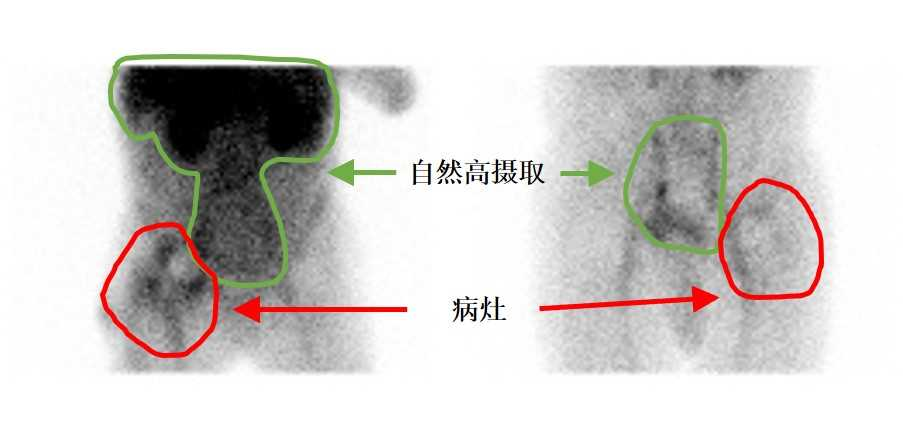
\includegraphics{figures/chap03_hip.jpg}
  \caption{髋关节置换手术后的动态骨显像}
  \label{fig:chap03_hip}
\end{figure}

(2)\textbf{髋关节置换手术后的动态骨显像存在着生理高摄取区域}。在人体的髋部附近存在着膀胱和肾脏这类自然高摄取区域,同时假体关节疼痛区域也会出现高摄取的情况,如图\ref{fig:chap03_hip}所示。这两者具有相似的图像特征,同时出现会导致神经网络在训练过程中产生混淆,无法学习到真实有用的信息,难以关注于病灶区域。

(3)\textbf{动态骨显像本身的影像特点}。动态骨显像包括三种不同条件下采集的影像,分别是在注射后立刻动态扫描(2秒/帧,20帧)用于获取灌注信息的血池相、灌注后动态扫描(1分钟/帧,5帧)可帮助诊断炎症状况或血液供应问题的血流相\cite{schauwecker1992scintigraphic}和在延迟代谢阶段中(示踪剂注射后4小时,1帧)扫描的延迟相。因此,主要存在的问题是需要确定要使用哪些相。

(4)\textbf{动态骨显像具有时间连续性}。动态骨显像中,每张图像拥有组织摄取形态特征,一系列图像之间在时序上存在生理代谢差异性变化特征。因此,如何利用动态骨显像的时序性特征也是一个需要研究的主要问题之一。

(5)\textbf{神经网络是一个缺乏解释的黑盒}。DBS-eNet是一个端到端的神经网络,可直接通过数据输入到模型之中获得最终结果。这导致医生很难以理解或者分析模型所提取和学习到的相关知识。这不仅缺乏决策过程中的透明性,还没有对模型的决策结果的解释,无法给医生带来可信度以及临床诊断的依据。

在本章研究中,设计了一个基于\(^{99m}\)TC-MDP动态骨显像的框架,用于辅助诊断假体关节感染。该框架针对上述问题一一进行优化改进:

(1)通过使用数据增强方法(镜像、旋转)和损失函数Focal Loss\cite{lin2017focal}上的改进(结合Label smoothing\cite{zhang2021delving}),来解决数据集规模小和数据不平衡的问题。

(2)提出了三种数据预处理算法,分别是标准预处理算法、干扰减少预处理算法和基于感兴趣区域预处理算法,来获取图像序列中有效的信息。其中,标准预处理算法可以用于经历过膝关节置换手术后患者的动态骨显像,同时这三种预处理算法都可以用于经历过髋关节置换手术后患者的动态骨显像。

(3)动态骨显像由血流相、血池相和延迟相组成。由于非感染与感染在延迟相中均可以呈现阳性,而血流相和血池相对于假体关节感染的诊断更具有敏感性。当血池相和血流相呈现阳性表明感染的可能性较大,当血池相和血流相呈现阴性的时候可以排除假体关节感染。由此,在专家的建议下,本章的研究主要关注于动态骨显像的血流相和血池相。

(4)针对动态骨显像的时序性图像序列特性,提出了一个基于深度学习和多特征的有效分类网络,DBS-eNet。该网络采用了三维深度卷积和卷积长短期记忆(Convolution Long Short Term Memory, ConvLSTM)\cite{shi2015convolutional}作为基础构建块,能够提取预处理后的动态骨显像的在影像学特征和时序特征,并且获得最终的预测结果。

(5)为了验证所提出框架的决策结果的有效性和可信度,在专家的建议下,本章引入了用于可视化模型对某一类输入图像的感兴趣区域的Grad-CAM(Gradient-weighted Class Activation Mapping)\cite{selvaraju2017grad}和用于可视化分类模型提取的特征的可区分性的t-SNE(t-distributed Stochastic Neighbor Embedding)\cite{van2008visualizing}。

\begin{figure}[htbp]
  \centering
  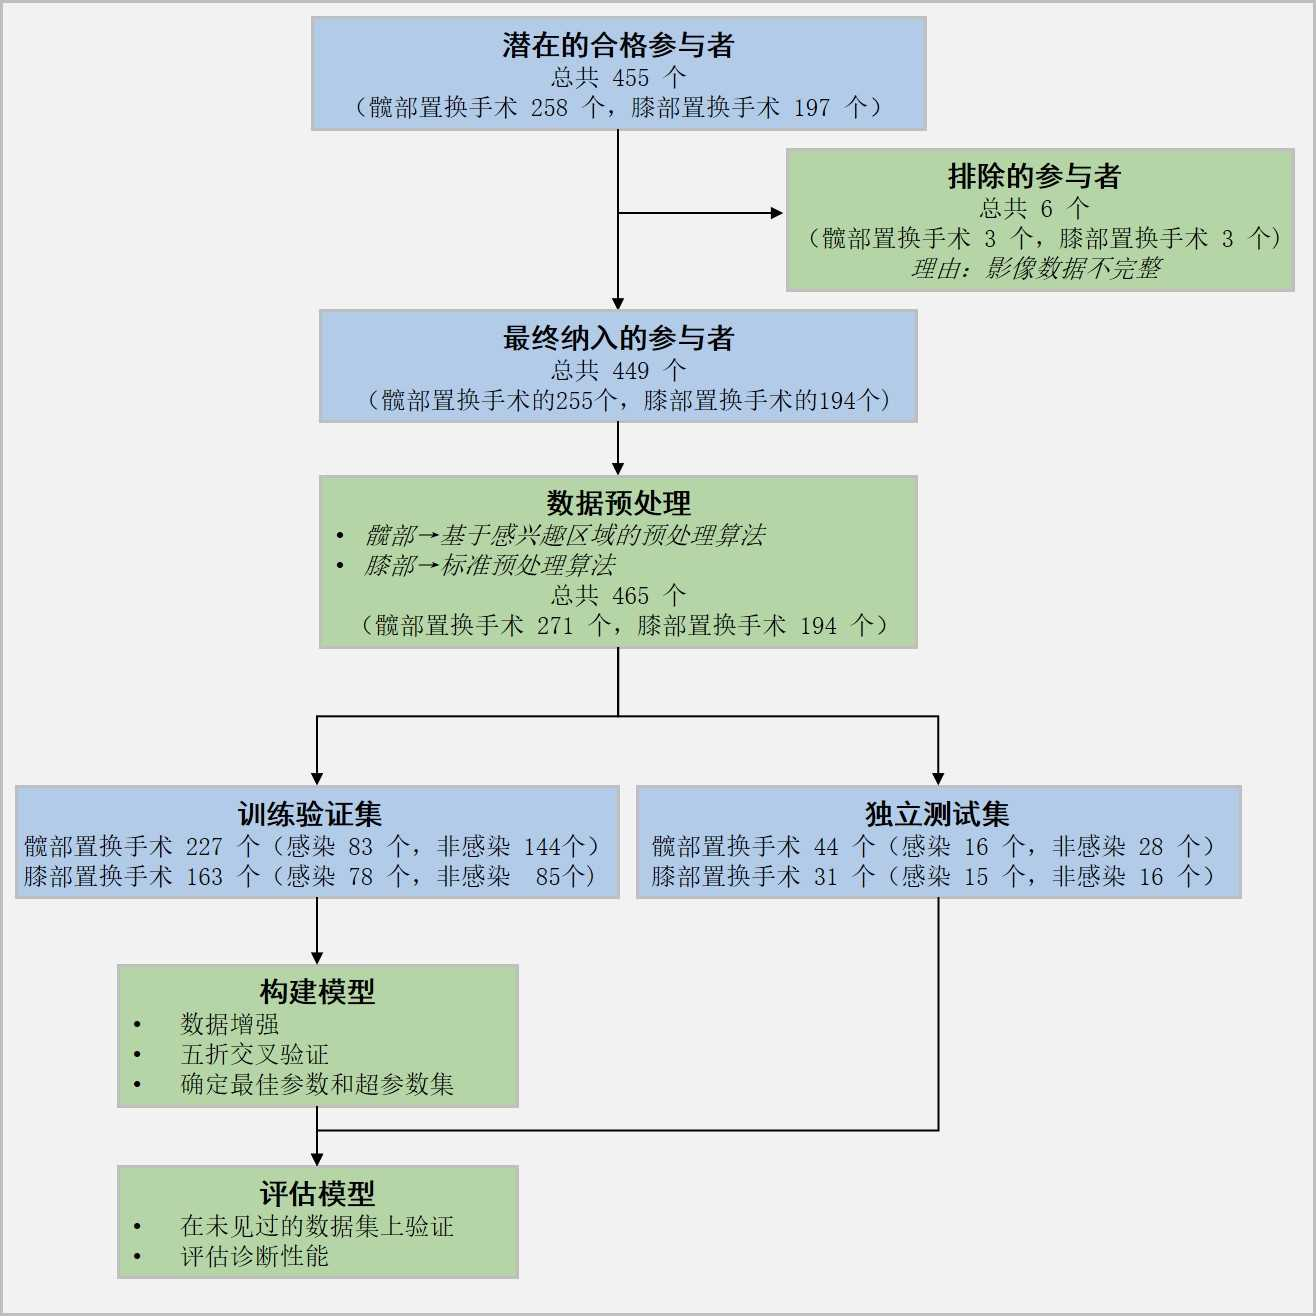
\includegraphics[width=\textwidth]{figures/chap03_workflow.jpg}
  \caption{研究的整体流程:蓝色框表示数据集的信息,绿色框表示对数据集的操作}
  \label{fig:chap03_workflow}
\end{figure}

本章研究的整体流程如图\ref{fig:chap03_workflow}所示。首先,通过最初的数据收集与筛选,最终得到了包含227个髋关节置换手术后的患者数据(感染组与非感染组:83 vs. 144)和163个膝关节置换手术后的患者数据(感染组与非感染组:78 vs. 85)的训练验证集,以及由44个髋关节置换手术后的患者数据(感染组与非感染组:16 vs. 28)和31个膝关节置换手术后的患者数据(感染组与非感染组:15 vs. 16)组成的独立测试集。其次,设计和改良模型结构。通过在训练验证集中五折交叉验证的结果,适应性地调整模型结构、超参数和训练策略,来获取最终的模型和最佳的超参数。最后,在独立测试集上采用分类任务中的评估指标进一步全面地评估模型的综合性能。

\section{数据预处理}

为了有效地解决动态骨显像数据规模较小、数据集不平衡以及存在自然高摄取区域的问题,本节设计了一个数据预处理流程,如图\ref{fig:chap03_preprocess}所示。通过该流程将动态骨显像转换成有效信息。具体流程如下:

(1)数据清洗与标注:对收集的经历过关节置换手术的患者数据进行清洗,并且进行类别、干扰区域、感兴趣区域的标注;

(2)预处理算法:需要将获取的原生数据转换成可有效区分的数据,去除掉自然高摄取区域的干扰;

(3)数据增强:通过镜像与旋转生成新的数据样本,来增加数据的多样性,以缓解数据集过小的问题。

\begin{figure}[htbp]
  \centering
  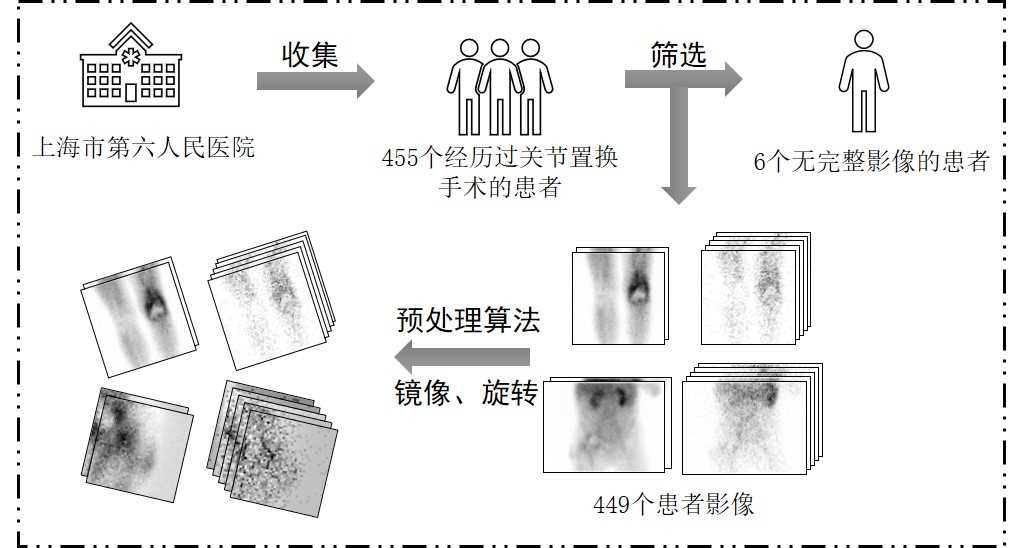
\includegraphics[width=0.9\textwidth]{figures/chap03_preprocess.jpg}
  \caption{针对动态骨显像的数据预处理整体流程示意图}
  \label{fig:chap03_preprocess}
\end{figure}

\subsection{数据清洗与标注}

本章所采集的动态骨显像数据都是以DICOM(Digital Imaging and Communications in Medicine)格式存储。DICOM被广泛用于存储、交换和传输医学图像。作为现代放射成像的核心,DICOM已被医院和医疗软件行业广泛采用,支持各种不同医疗设备获取的影像模态,如超声、CT和MRI等\cite{mildenberger2002introduction}。

数据预处理的第一步是对收集到的患者数据进行清洗,如排除掉影像数据不完整、缺乏完整诊断结果的病例。此外,为了保护病人的个人隐私信息,对DICOM格式文件进行脱敏。因此,DICOM格式文件仅仅保留与图像数据相关的信息。在经过上述操作后,本文作者在专业的核医学医生的指导下使用ITK-SNAP软件(v3.8.0,http://www.itksnap.org)对所有的经历过关节置换手术的患者的动态骨显像进行标注,并最终标注结果由专业医生进行了核查。标注根据患者治疗过程中获取的诊断报告为依据,为每一个患者的动态骨显像确定病灶的类别信息和位置信息,还为经历过髋关节置换手术的患者的动态骨显像标注了干扰区域和感兴趣区域,如图\ref{fig:chap03_label}所示。

\begin{figure}[htbp]
  \centering
  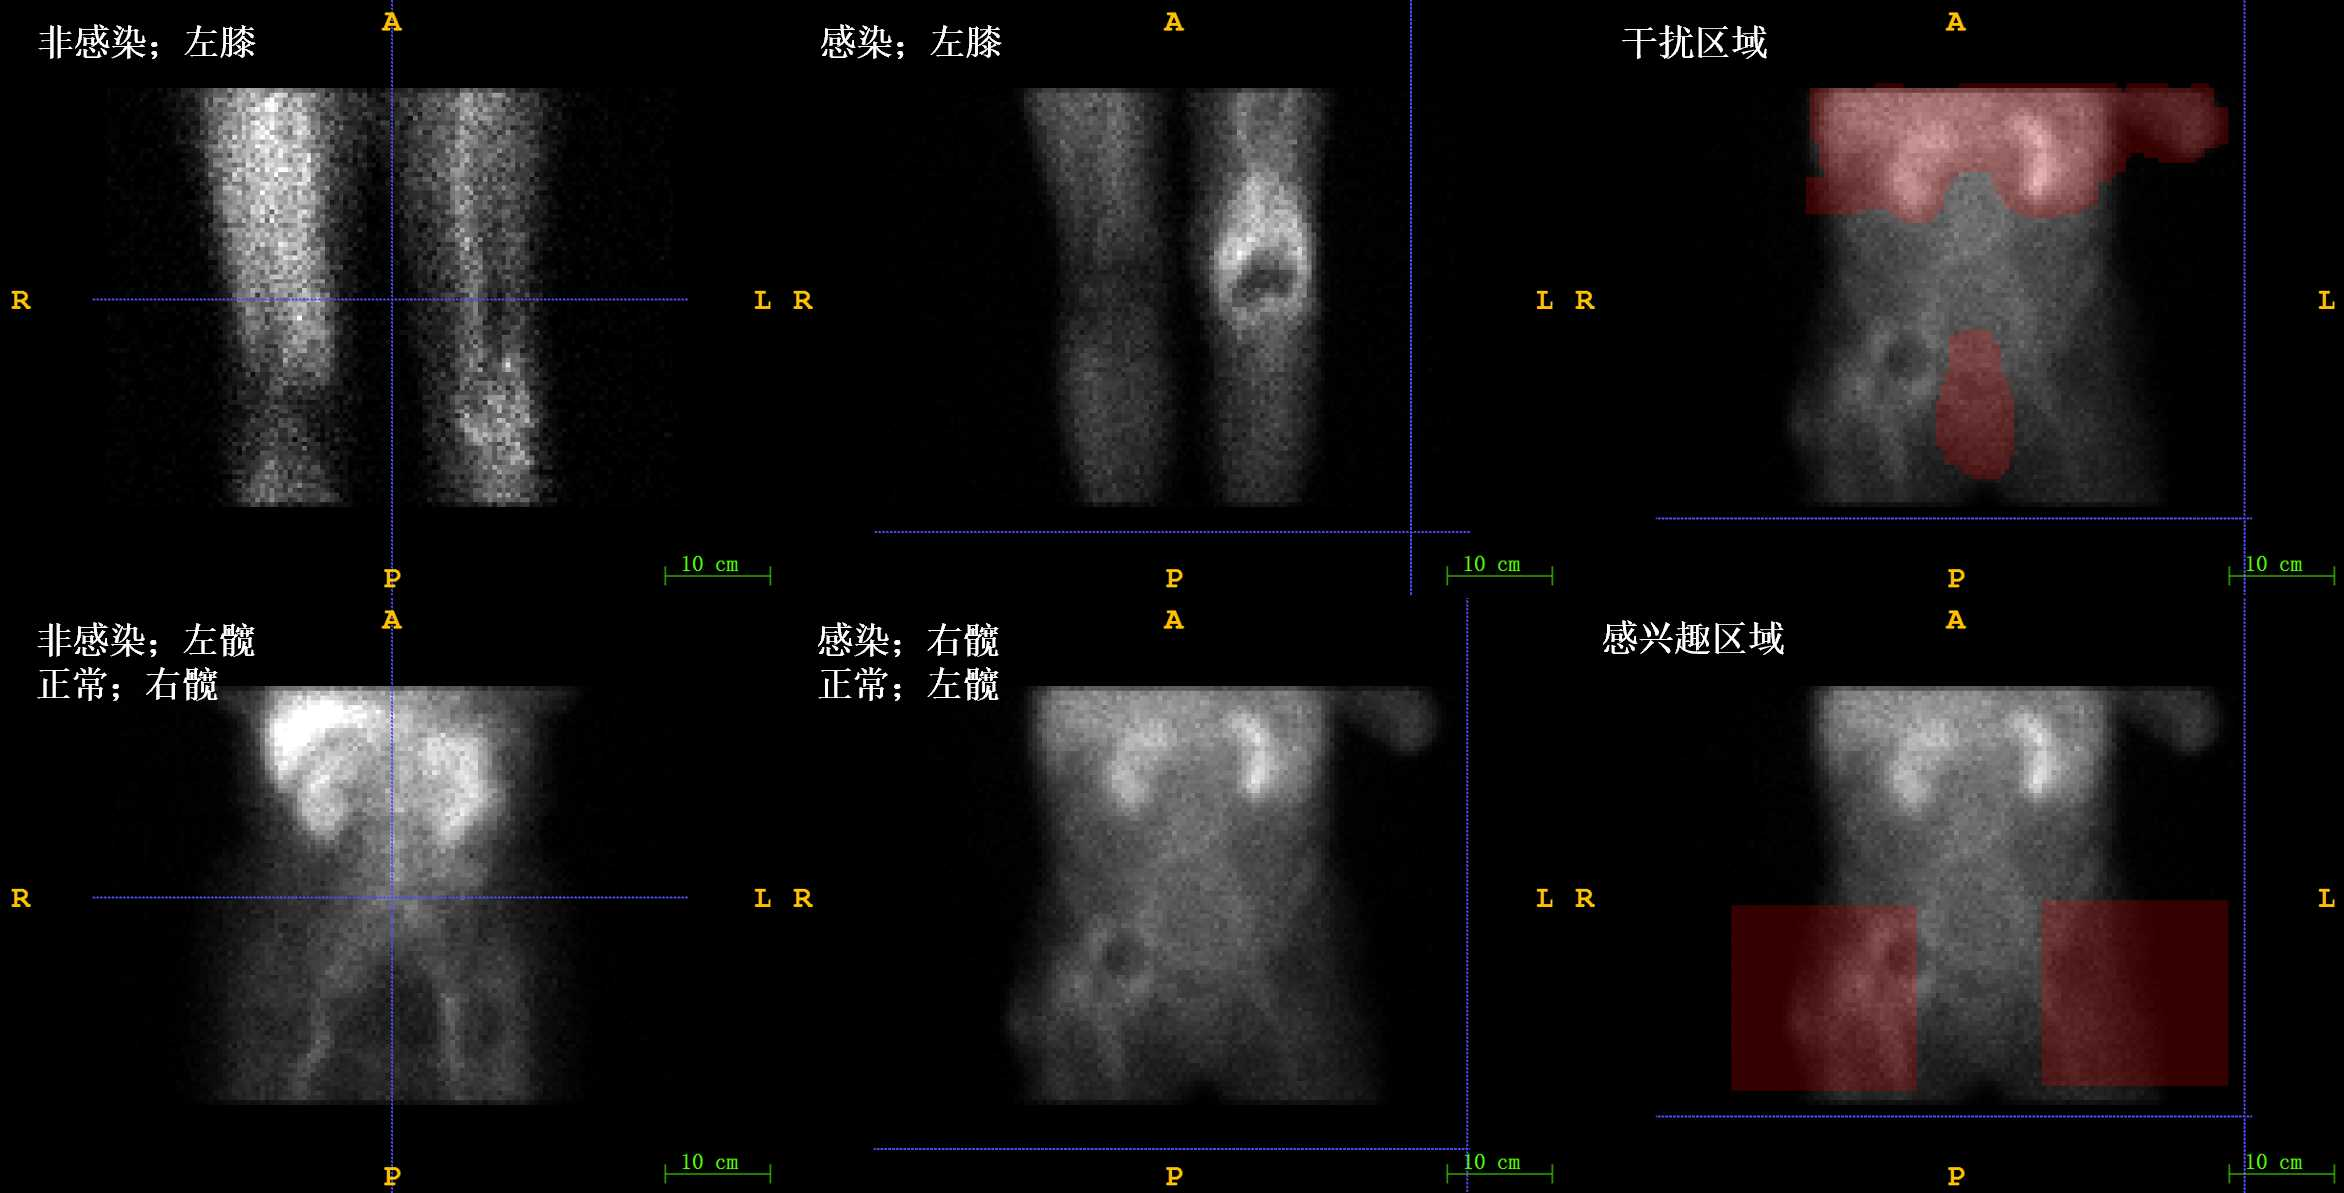
\includegraphics[width=\textwidth]{figures/chap03_label.jpg}
  \caption{动态骨显像的数据标注}
  \label{fig:chap03_label}
\end{figure}

在数据标注完成之后,将对数据进行进一步的整理工作。首先,去除掉数据集中存在的重复的影像数据。其次,将所有的影像数据和标注数据转换为NPZ格式。其中,NPZ格式文件是NumPy\cite{harris2020array}中的一种以二进制的形式存储的格式文件,可用于以未压缩形式的存储多个NumPy数组对象。通过采用NPZ格式文件,将影像数据与它对应的标注数据存放在一个NPZ文件之中。

\subsection{预处理算法}

由于原生的影像数据在不同个体之间的数值波动范围差异大以及存在自然高摄取区域,会极大地影响分类性能。因此,本节提出了三种预处理算法,将动态骨显像的影像数据转换为有效信息。预处理后得到的影像数据通过可视化后如图\ref{fig:chap03_algorithm}所示。

\begin{figure}
  \centering
  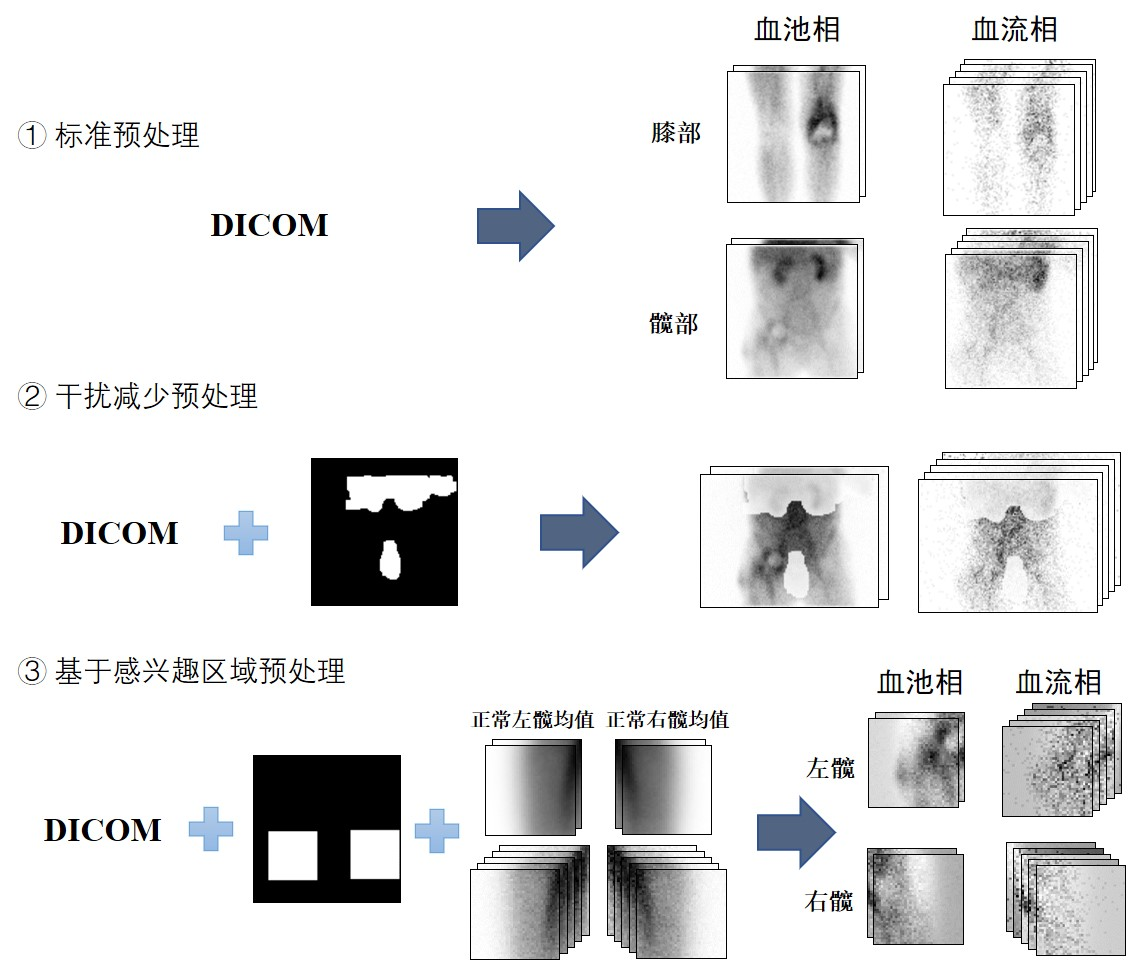
\includegraphics[width=0.9\textwidth]{figures/chap03_algorithm.jpg}
  \caption{三种预处理算法得到的有效信息示意图}
  \label{fig:chap03_algorithm}
\end{figure}

(1)标准预处理

标准预处理的关键步骤就是执行最小最大归一化,通过设定图像数据的下限和上限来调整数据的范围。其基本原理在于病灶区域的上限往往显著高于一般的正常区域,而一般的正常区域的数值范围相对较为固定,因此通过调整图像数据的上限,能够更好地突显出潜在的病灶区域,提高模型对于病灶特征的感知能力。标准预处理算法过程如下:

读取\(^{99m}\)Tc-MDP动态骨显像中的血流相\(F\)和血池相\(P\)。其中,血流相\(F\)一共有20张\(128 \times 128\)的二维图像,而血池相\(P\)一共有5张\(128 \times 128\)的二维图像。随后计算出血流相和血池相中的最大值,如公式\ref{eq:chap03_maxmin}:
\begin{equation}
  \begin{aligned}
    F_{max} & = max(max(F_1), max(F_2), \cdots, max(F_{20})) \\
    P_{max} & = max(max(P_1), max(P_2), \cdots, max(P_5))
  \end{aligned}
  \label{eq:chap03_maxmin}
\end{equation}

最后,分别对血流相和血池相数据进行截断和归一化处理,如公式\ref{eq:chap03_standard}所示。
\begin{equation}
  \begin{aligned}
    F_i^{m, n} & =
    \begin{cases}
      1,                           & \text{if \(F_i^{m, n} \geq \alpha F_{max} \)} \\
      0,                           & \text{if \(F_i^{m, n} \leq 0\)}               \\
      F_i^{m, n} / \alpha F_{max}, & \text{otherwise}
    \end{cases} \\
    P_j^{m, n} & =
    \begin{cases}
      1,                           & \text{if \(P_j^{m, n} \geq \alpha P_{max} \)} \\
      0,                           & \text{if \(P_j^{m, n} \leq 0\)}               \\
      P_j^{m, n} / \alpha P_{max}, & \text{otherwise}
    \end{cases}
  \end{aligned}
  \label{eq:chap03_standard}
\end{equation}
其中,\( 1 \leq i \leq 20, 1 \leq j \leq 5, 1 \leq m, n \leq 128 \),\(i, j\)分别表示血流相和血池相中相应序号的图像,\(m, n\)分别表示二维图像中像素的行坐标和列坐标,\(alpha \in [0,1]\)是自定义的超参数,用于调整归一化区间的最大值,默认值为\(0.5\)。

(2)干扰减少预处理

干扰减少预处理在标准预处理的基础上,考虑到了自然高摄取区域这类干扰区域,如肾脏、膀胱,与高摄取的病灶区域具有一定的相似性,减少了神经网络对干扰区域与病灶区域的混淆,用以提升分类模型的性能。对于动态骨显像中的多张二维影像数据,每个值表示在相应的人体位置上吸收药物的大致放射强度。该值越大,表示此处药物吸收得多,代表着此处的生理代谢更加活跃。因此,干扰减少预处理的基本原理是降低自然高摄取区域的放射强度值来减少它的干扰能力。干扰减少预处理算法过程如下:

与标准预处理类似,首先读取动态骨显像中的血流相\(F\)和血池相\(P\)并计算出血流相和血池相中的最大值。然后,使用公式\ref{eq:chap03_Interference_reduction}通过干扰区域\(A_{IR}\)来降低自然高摄取区域的放射强度:
\begin{equation}
  \begin{aligned}
    F_i^{m, n} & =
    \begin{cases}
      \alpha_{IR}F_i^{m, n}, & \text{if \((m,n) \in A_{IR}\)} \\
      F_i^{m, n},            & \text{otherwise}
    \end{cases} \\
    P_j^{m, n} & =
    \begin{cases}
      \alpha_{IR}P_j^{m, n}, & \text{if \((m,n) \in A_{IR}\)} \\
      P_j^{m, n},            & \text{otherwise}
    \end{cases}
  \end{aligned}
  \label{eq:chap03_Interference_reduction}
\end{equation}
其中,\(\alpha_{IR} \in [0, 1]\)表示对干扰区域的衰竭程度,默认值为\(0.4\)。

最后,再通过标注预处理中公式\ref{eq:chap03_standard}分别对血流相和血池相数据进行截断和归一化处理。

(3)基于感兴趣区域预处理

基于感兴趣区域预处理来源于核医学医生在诊断过程中通过分析正常髋部与关节置换手术后的髋部之间的差异做出决策。由此,通过基于感兴趣区域处理后将得到差异特征,不同于标准预处理和干扰减少预处理得到的强度特征。基于感兴趣区域预处理的算法过程如下:

首先,根据标注的大小为\(40 \times 40\)的感兴趣区域,从动态骨显像中将该区域裁剪出来。其次,根据类别信息\(c\)和位置信息\(p\),计算正常的左髋和右髋的平均值,如公式\ref{eq:chap03_normalL}和\ref{eq:chap03_normalR}所示。
\begin{equation}
  \begin{aligned}
    FNL_{i}^{m, n} & = mean(\sum_{c_i = \text{正常}, p_i = \text{左} } F_i^{n, m}) \\
    PNL_{i}^{m, n} & = mean(\sum_{c_i = \text{正常}, p_i = \text{左} } P_i^{n, m})
  \end{aligned}
  \label{eq:chap03_normalL}
\end{equation}
\begin{equation}
  \begin{aligned}
    FNR_{i}^{m, n} & = mean(\sum_{c_i = \text{正常}, p_i = \text{右} } F_i^{n, m}) \\
    PNR_{i}^{m, n} & = mean(\sum_{c_i = \text{正常}, p_i = \text{右} } P_i^{n, m})
  \end{aligned}
  \label{eq:chap03_normalR}
\end{equation}
其中,\(i, j, m, n\)与公式\ref{eq:chap03_standard}一致,\(FNL, PNL\)分别表示正常左髋血流相和血池相的平均值,\(FNR, PNR\)分别表示正常右髋血流相和血池相的平均值。

最后,对于其他的经历过关节置换手术的感兴趣区域的血流相和血池相\(FROI, PROI\),将根据公式\ref{eq:chap03_roi}进行计算,获得与正常髋部之间的差异特征。
\begin{equation}
  \begin{aligned}
    FROI_i^{m, n} & =
    \begin{cases}
      FROI_i^{m, n} - FNL_i^{m, n}, & \text{if \(pROI_i = \)左} \\
      FROI_i^{m, n} - FNR_i^{m, n}, & \text{if \(pROI_i = \)右}
    \end{cases} \\
    PROI_i^{m, n} & =
    \begin{cases}
      PROI_i^{m, n} - PNL_i^{m, n}, & \text{if \(pROI_i = \)左} \\
      PROI_i^{m, n} - PNR_i^{m, n}, & \text{if \(pROI_i = \)右}
    \end{cases}
  \end{aligned}
  \label{eq:chap03_roi}
\end{equation}
其中,\(pROI_i\)表示经历过关节置换手术的髋部的位置信息。

\subsection{数据增强}

由于数据集规模较小,为了补充数据集,本节采用了镜像和旋转的方式来对生成新的训练样本。镜像将对整个动态骨显像的血流相和血池相进行相同的水平翻转,同时旋转也是对整个动态骨显像的血流相和血池相从\(-20^{\circ}\)到\(20^{\circ}\)中随机选取一个角度进行旋转。数据增强采用在线策略,即在训练过程中随机地应用在预处理后得到的强度特征或者差异特征。在本章研究中,所有的数据增强方法都将以50\%的概率进行采用。

\section{DBS-eNet}

动态骨显像拥有两个具有时序的血流相和血池相,它们展示了一个患者在注射药剂后不同时间点下的状态。由于CNN和ConvLSTM在提取特征能力上拥有各自的适用领域,本章提出了结合了CNN和ConvLSTM的DBS-eNet。该模型设计了卷积对输入的特征进行下采样和图像特征提取,有助于减少模型的计算量和参数量,并且采用了ConvLSTM继续丰富图像特征并提取时序特征。卷积和ConvLSTM的组合可以增强对动态骨显像的特征提取能力,为模型提供图像以及时序上的混合特征信息。

\subsection{模型结构}

\begin{figure}[H]
  \centering
  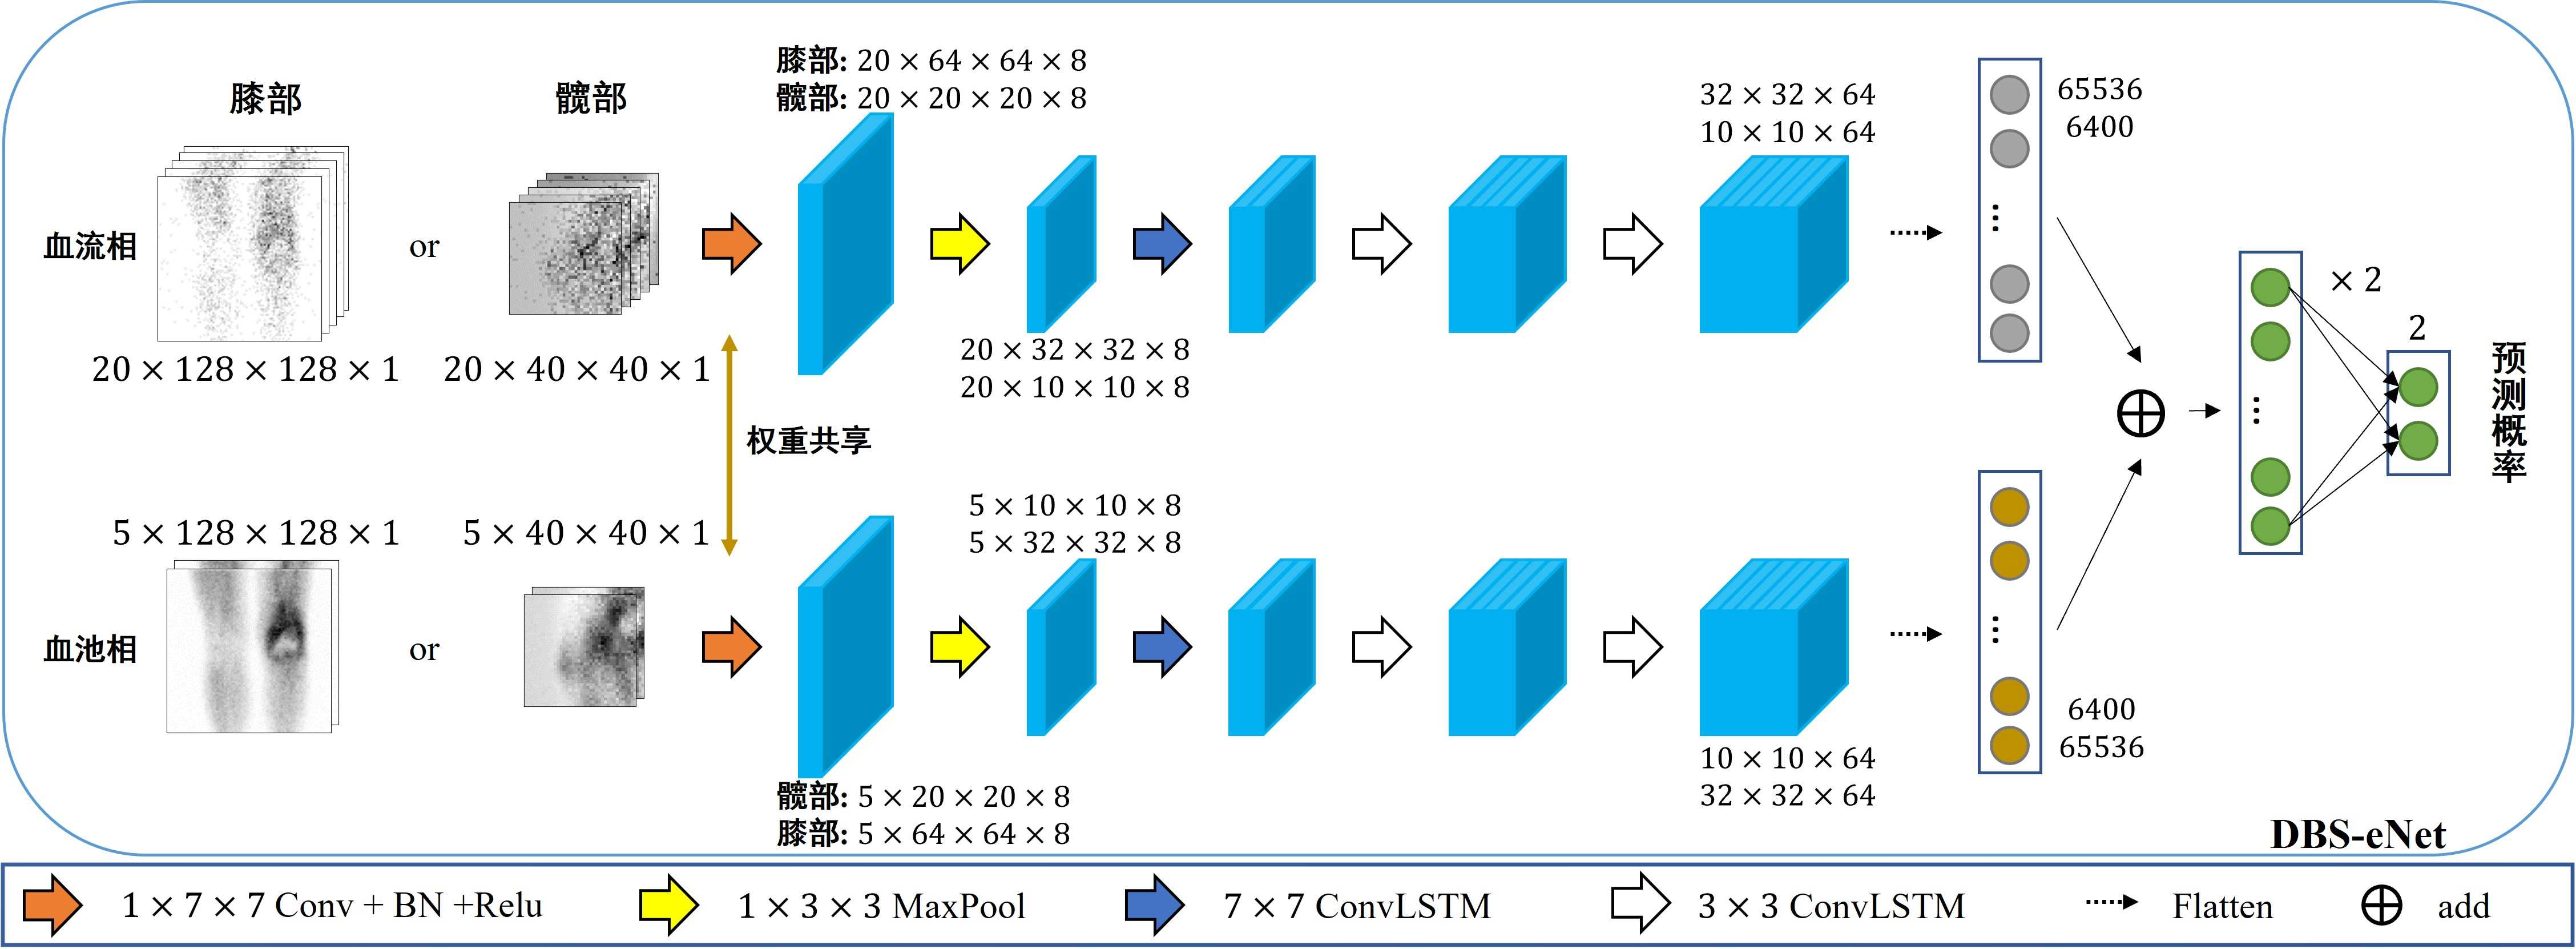
\includegraphics[width=\textwidth]{figures/chap03_framework.jpg}
  \caption{基于深度学习的多特征神经网络模型(DBS-eNet)}
  \label{fig:chap03_framework}
\end{figure}

根据动态骨显像的具有时序性的单通道二维图像,针对性地构建了基于深度学习和多特征的有效分类网络DBS-eNet的三个部分。模型结构如图\ref{fig:chap03_framework}所示。

第一部分是一个共享权重且用于提取生理摄取形态特征的\(1 \times 7 \times 7\)的三维卷积层、批归一化层(Batch Normalization)\cite{ioffe2015batch}、校正线性单元(Rectified Linear Unit,ReLU)和用于下采样的最大池化层(Max Pooling)组成。其中,\(1 \times 7 \times 7\)三维卷积层是时序卷积,在时序维度上权重的尺寸为1,等价于对每一张图像进行特征提取。又由于血流相和血池相是一个患者在不同时间点下的状态,即在血流相和血池相上病灶区域处于同一位置,因此,时序卷积设定为共享权重的形式,去提取血流相和血池相上每一张图像中同一病灶的特征,同时减少参数量;批归一化层用在卷积层之后可以避免数据分布发生变化,用以保留网络各层在训练过程中的学习成果;ReLU激活函数可以有效解决梯度消失的问题并加快模型的收敛速度;最大池化层则可以减少特征的维度的同时提取出特征中更好更强的语义信息。第一部分这样的设计,可以在减少参数量和计算量的同时保持特征的主要语义信息。

第二部分是一个由一层\(7 \times 7\)的ConvLSTM和两层\(3 \times 3\)的ConvLSTM组成。这一设计旨在通过ConvLSTM的结构,在图像处理的过程中更加全面地捕捉和丰富生理形态摄取特征并且在图像序列之中捕获生理代谢差异变化特征。首先,\(7 \times 7\)的ConvLSTM通过更大的感受野去有效丰富影像中病灶的摄取形态特征。接着,两层\(3 \times 3\)的ConvLSTM以较小的卷积核去捕捉到病灶摄取形态中的各种细节和纹理特征。最后,通过引入时序感知的ConvLSTM,网络不仅可以更好地理解单一图像的内容,还能够在图像序列中建模和捕捉时间上的关联性,从而更全面地分析病灶区域中药剂的摄取形式和程度变化。因此,第二部分在图像特征的丰富性和时序特征的捕获上取得了良好的平衡,为整个网络的性能提供了更强大的表达能力。

第三部分是特征融合层和两层全连接层,融合来自于血流相和血池相中提取的图像特征和时序特征来计算最终诊断结果的概率。首先,特征融合层通过逐元素地融合来更全面、准确地反映动态骨显像中图像序列的复杂特征。接着,第一层全连接层引入GELUs(Gaussian error linear units)和Dropout\cite{srivastava2014dropout}。GELUs有助于于引入非线性元素,增强网络对特征的表达能力,同时Dropout则在一定程度上减轻了过拟合的风险,提供了模型的泛化能力。最后,第二层全连接层的输出经过Dropout层的处理,进一步强化了网络对复杂特征的建模能力。第三部分通过这样的设计,有助于确保网络在处理两个相的时序图像特征时保持稳健性,提供可靠而精准的结果。

\subsection{ConvLSTM}

ConvLSTM是DBS-eNet网络中的核心模块。由于动态骨显像是一个图像序列,重要的不仅是图像特征,还需要捕获整体图像序列之间的时序特征。因此,与普通的卷积神经网络相比,卷积与LSTM相结合的ConvLSTM能够捕获到动态骨显像中的时空特征,更加有效地处理复杂的时序信息,从而使网络在分析动态骨显像时表现得更为出色。

在常见的序列建模模型中,LSTM\cite{memory2010long}作为一种特殊的RNN结构,专门设计来解决传统RNN中存在的梯度消失或梯度爆炸的问题,且已经被证明在建模远程依赖关系方面是稳定而强大的。通过记忆单元和门控机制来控制信息的流动,可以将梯度留在记忆单元之中,防止梯度太快消失,以更有效地捕捉长期依赖关系。LSTM的关键公式如\ref{eq:chap03_lstm}所示。
\begin{equation}
  \begin{aligned}
    i_t & = \sigma(W_i x_t + U_i h_{t-1} + b_i)                                    \\
    f_t & = \sigma(W_f x_t + U_f h_{t-1} + b_f)                                    \\
    o_t & = \sigma(W_o x_t + U_o h_{t-1} + b_o)                                    \\
    c_t & = f_t \odot c_{t-1} + i_t \odot \text{Tanh}(W_c x_t + U_c h_{t-1} + b_c) \\
    h_t & = o_t \odot \text{Tanh}(c_t)
  \end{aligned}
  \label{eq:chap03_lstm}
\end{equation}
其中,\(i_t,f_t,o_t,h_t,c_t\)分别表示\(t\)时刻下的输入们、遗忘门、输出门、隐藏状态和记忆单元,\(\odot\)表示逐元素相乘。多个LSTMs可以堆叠起来形成更加复杂的结构,用以解决更多更复杂的序列建模任务。

尽管LSTM可以解决序列建模任务,但是记忆单元中的状态信息和输出都是一个数值,无法处理更加复杂的序列问题。为了解决这个问题,FC-LSTM\cite{graves2013generating}被提出来,其中它的输入、状态信息和输出均是一维向量。而ConvLSTM在FC-LSTM的基础上进行了扩展,将将输入到状态和状态到状态的转换过程中的全连接结构转换成了卷积结构。为了更好地处理时空数据,ConvLSTM在设计上的显著区别在于输入\(\mathcal{X}_t\)、记忆单元的输出\(\mathcal{H}_t\)和状态信息\(\mathcal{C}_t\)都是二维数据,即空间维度。为了更好地理解输入和状态信息,可以将它们视为一个空间网格。ConvLSTM通过输入和状态信息的局部邻域来确定网格中某个位置的未来状态。这可以很简单地通过卷积操作来实现状态到状态和输入到状态的转变。ConvLSTM的关键公式如\ref{eq:chap03_convlstm}所示。
\begin{equation}
  \begin{aligned}
    i_t           & = \sigma(W_{xi} \ast \mathcal{X}_t + W_{hi} \ast \mathcal{H}_{t-1} + W_{ci} \odot \mathcal{C}_{t-1} + b_i)          \\
    f_t           & = \sigma(W_{xf} \ast \mathcal{X}_t + W_{hf} \ast \mathcal{H}_{t-1} + W_{cf} \odot \mathcal{C}_{t-1} + b_f)          \\
    \mathcal{C}_t & = f_t \odot \mathcal{C}_{t-1} + i_t \odot \text{Tanh}(W_{xc} \ast \mathcal{X}_t + W_{hc} * \mathcal{H}_{t-1} + b_c) \\
    o_t           & = \sigma(W_{xo} \ast \mathcal{X}_t + W_{ho} \ast \mathcal{H}_{t-1} + W_{co} \odot \mathcal{C}_{t} + b_o)            \\
    \mathcal{H}_t & = o_t \odot \text{Tanh}(\mathcal{C}_t)
  \end{aligned}
  \label{eq:chap03_convlstm}
\end{equation}
其中,\(\ast\)表示为卷积计算,\(\odot\)表示逐元素相乘。为了确保状态信息在计算过程中空间大小不变且与输入相同,在进行卷积计算之前需要进行填充(padding)。

\subsection{损失函数}

损失函数用于假体关节感染任务中的作用是评估DBS-eNet网络模型结果的准确程度。由于任务本身收集的髋部数据中存在类别不平衡的情况,不同类别的样本数量差异较大,这可能导致模型学习过程中存在一定的偏差。由于感染与非感染的样本分布不均匀,模型可能更容易偏向于在数量中占主导地位的类别,而对于少数类别的样本学习效果相对较弱。为了解决这一问题,本章引入并设计了带有标签平滑(Label smoothing)\cite{zhang2021delving}的\(\alpha\)平衡版的Focal Loss\cite{lin2017focal}用于髋关节置换手术的差异特征信息,解决类别不平衡与类别之间的相似性,如公式\ref{eq:chap03_THALoss}所示。
\begin{equation}
  \begin{aligned}
    \tilde{y}_{n, c}      & =  \text{Softmax}(x_{n, c}) = \frac{\exp(x_{n, c})}{\sum_{i = 1}^{C}\exp(x_{n, i})}                                                                       \\
    y_{n, c}              & =
    \begin{cases}
      1 - \epsilon         & \text{if \(c = \mathcal{C}\)}    \\
      \frac{\epsilon}{C-1} & \text{if \(c \neq \mathcal{C}\)}
    \end{cases}                                                                                                                \\
    \mathcal{L}_{fl}(x,y) & = -\frac{1}{N}\sum_{n=1}^N \alpha_{n,\mathcal{C}} \cdot (1 - \sum_{c=1}^C \tilde{y}_{n,c}y_{n,c})^{\gamma} \cdot \log\sum_{c=1}^{C}\tilde{y}_{n,c}y_{n,c}
  \end{aligned}
  \label{eq:chap03_THALoss}
\end{equation}
其中,\(x_{n,c}\)是模型的输出结果,表示样本\(n\)对于类别\(c\)的预测值;\(\tilde{y}_{n, c}\)是\(x_{n,c}\)经过Softmax后的预测结果;\(C\)表示类别数量;\(y_{n,c}\)是标签平滑后的真实标签值;\(\epsilon\)是平滑参数;\(\mathcal{C}\)表示正确的类别;\(\alpha_{n,\mathcal{C}}\)表示样本\(n\)对于所属类别\(\mathcal{C}\)的权重因子;\(\gamma \geq 0\)表示可调聚焦参数;\(N\)表示批大小。

而对于类别更为平衡的膝关节置换手术的强度特征信息,则采用了如公式\ref{eq:chap03_TKALoss}所示的加权交叉熵损失函数。
\begin{equation}
  \begin{aligned}
    y_{n, c}         & =
    \begin{cases}
      1 & \text{if \(c = \mathcal{C}\)}    \\
      0 & \text{if \(c \neq \mathcal{C}\)}
    \end{cases}                                         \\
    \mathcal{L}_{ce} & = -\frac{1}{N}\sum_{n=1}^N\sum_{c=1}^C w_c\log\tilde{y}_{n,c}y_{n,c}
  \end{aligned}
  \label{eq:chap03_TKALoss}
\end{equation}
其中,\(\tilde{y}_{n, c},y_{n,c},C,\mathcal{C},N\)同上式\ref{eq:chap03_THALoss}一致;\(w_c\)表示对于类别\(c\)的权重因子。

\subsection{可视化模块}

为了了解DBS-eNet的决策基础,采用了Grad-CAM和t-SNE。Grad-CAM是一种用于解释深度学习模型预测的可视化技术,特别适用于图像分类任务。其基本原理是在模型通过前向传播预测后计算反向传播的梯度,随后通过对梯度进行全局平均池化得到相应特征图的权重生成类激活图。本章将Grad-CAM应用在框架中的DBS-eNet最后一个ConvLSTM层上来计算类激活图。该类激活图可以显示出动态骨显像中不同区域的重要性。t-SNE是一种降维和可视化高维数据的技术。其核心思想是通过在低维空间中保留原始数据点之间的相似性关系,将高维数据映射到一个更易于理解和可视化的低维空间。本章通过采用保持不同样本之间相对距离的t-SNE方法,将DBS-eNet中提取的最后的特征向量(1024维)降至2维,并将其可视化在二维散点图上来显示出该特征向量的有效性和可区分性。其中,每个点代表在特征空间中的一个感染者或者非感染者的样本。

\section{实验}

\subsection{实验环境}

\begin{table}[htbp]
  \centering
  \caption{实验配置}
  \begin{tabular}{cc}
    \toprule
    环境         & 配置                                     \\
    \midrule
    操作系统     & Linux Ubuntu 20.04.2                     \\
    CPU          & Intel(R) Xeon(R) Gold 5115 CPU @ 2.40GHz \\
    GPU          & NVIDIA Tesla V100, 32GB                  \\
    内存         & 128GB                                    \\
    编程语言     & Python 3.8.17                            \\
    深度学习框架 & Pytorch 1.8.0                            \\
    \bottomrule
  \end{tabular}
  \label{tab:chap03_experimental_config}
\end{table}

本章中的所有实验均在PAI上海大学机器学习平台上进行。该平台是由上海大学计算机学院设计和构建的多加速器异构集群。PAI平台是上海大学首台采用自主开发的基于容器的PAI管理系统的异构计算平台,专注于支持机器学习和深度学习的科研和教学活动。自2018年6月以来,该平台一直提供稳定的计算服务。在硬件方面,该平台包括2个登录/管理节点、1套KNL计算节点、2个FPGA节点、10个双GPU节点、1台配备四个GPU的DGX-station、4个I/O节点,以及一套200T光纤存储阵列,同时配备有1套100G IB高速网络、1套100G OPA高速网络和1套千兆管理网络。这一多样化的硬件配置为各种计算需求提供了灵活的支持。平台的管理软件由上海大学计算机学院自主开发完成,学生们负责相应的软件维护和升级工作。PAI平台不仅面向全校师生提供了丰富的教学资源,还为各类计算任务提供了强大的计算服务。本章的实验的软硬件配置的详细信息如\ref{tab:chap03_experimental_config}所示。

\subsection{数据集}

\begin{table}[htbp]
  \centering
  \caption{动态骨显像的分布情况}
  \begin{tabular}{lcc}
    \toprule
    标签   & 髋关节置换手术 & 膝关节置换手术 \\
    \midrule
    感染   & 99             & 93             \\
    非感染 & 156            & 101            \\
    \bottomrule
  \end{tabular}
  \label{tab:chap03_dataset}
\end{table}

本文作者与上海市第六人民医院核医学科进行合作构建了假体关节感染动态骨显像数据集。该数据集包含髋关节置换手术和膝关节置换手术后的动态骨显像,分类详情见表\ref{tab:chap03_dataset}所示,一共纳入了从2016年1月至2021年6月之间455例具有最终诊断结果的患者,其中258名患者经历了髋关节置换手术,197名患者经历了膝关节置换手术。在查看了所有患者的影像后,其中6例患者由于影像不全被排除。最终纳入并分析了449例患者。所有患者在经历了膝关节置换手术或髋关节置换手术后均出现疼痛或关节功能障碍,且都进行了翻修手术。假体关节感染的最终诊断结果主要基于2021年的EBJIS的定义\cite{mcnally2021ebjis}。在本章的数据集中,一共有192例感染患者和257例非感染患者。

\subsection{评估指标}

假体关节感染诊断任务属于分类问题,本章选用了分类任务中常用的评估指标,如准确率(Accuracy,Acc)、特异率(Specificity,Spec)、敏感率(Sensitivity,Sen)、F1值(F1 Score),阴性预测值(Negative Predictive Value,NPV)、阳性预测值(Positive Predictive Value,PPV)和接收者操作特征曲线下面积(Area Under the receiver operating characteristic Curve,AUC),如式\ref{eq:chap03_metric}所示。
\begin{equation}
  \begin{aligned}
    Acc  & = \frac{TP+TN}{Total}                                         & F1  & = \frac{2 \times PPV \times Sen}{PPV + Sen} \\
    Spec & = \frac{TN}{TN+FP}                                            & Sen & = \frac{TP}{TP+FN}                          \\
    NPV  & = \frac{TN}{TN+FP}                                            & PPV & = \frac{TP}{TP+FP}                          \\
    AUC  & = \frac{\sum_{i \in P} rank_i - \frac{M(1+M)}{2}}{M \times N} &     &
  \end{aligned}
  \label{eq:chap03_metric}
\end{equation}
其中,\(TP,TN,FP,FN\)分别是真阳性、真阴性、假阳性、假阴性样本的数量;\(Total\)表示样本的整体数量;\(P\)表示阳性的类别;\(M,N\)分别是阳性样本和阴性样本的数量;\(rank_i\)是第\(i\)个样本的序号,所有的预测样本根据阳性预测值从小到大进行排序。

准确率表示对假体关节感染预测准确的样本在总样本的占比,但在样本不均衡的情况下,不能够很好地评估模型性能的优劣。特异率表示对实际不患有假体关节感染的患者诊断为未感染的概率。敏感率表示对实际上患有假体关节感染的患者诊断为感染的概率。阳性预测值表示为被诊断为感染的患者实际上患有假体关节感染的概率。阴性预测值表示为被诊断为未感染的患者实际上未患有假体关节感染的概率。F1值是阳性预测值和敏感率的综合评价指标。AUC是敏感性和特异性的综合评价指标。

此外,本章采用了Bootstrap\cite{hesterberg2011bootstrap}来计算这些评估指标的置信区间,并采用麦克内马尔检验(McNemar test)\cite{lachenbruch2014mcnemar}进行统计学分析,来验证DBS-eNet与专业的核医学医生之间的差异性。更进一步地采用了校准曲线(Calibration Curve)和决策曲线分析(Decision Curve Analysis,DCA)\cite{vickers2006decision}来更加全面地评估本章框架的潜在应用价值和有效性。校准曲线可以描绘模型输出的概率与实际观察到的事件发生概率之间的关系,在本章研究中用于评估DBS-eNet预测假体关节感染的概率与实际假体关节感染的概率之间的一致性。决策曲线分析是一种用于评估预测模型在不同概率阈值下对决策效果的方法。它通常应用于医学领域,特别是在评估临床预测模型的效果,决策曲线分析有助于确定模型在不同概率阈值下相对于其他决策策略的净收益,并为医学决策提供了实用的信息。

\subsection{实验结果}

实验中,对于构建的动态骨显像数据集先进行上述中的数据预处理后,可以从经历了髋关节置换手术的患者的动态骨显像中获得差异特征(\(25\times40\times40\))以及从经历了膝关节置换手术的患者的动态骨显像中获得强度特征(\(25\times128\times128\)),用于模型训练。对于模型的训练配置,采用了标准的随机梯度下降(Stochastic Gradient Descent,SGD)优化器,初始的学习率设置为0.01,动量(momentum)为0.8,权重衰减(weight decay)为0.0005。批大小(batch size)设置为4,Dropout的比例设置为0.2,以及整个训练周期(epoch)的数量为80。在训练周期的一半和四分之三,学习率将乘以0.1。

\begin{table}[htbp]
  \centering
  \caption{髋关节置换手术数据集上不同预处理算法下的准确率}
  \begin{tabular}{lcc}
    \toprule
                         & 五折交叉验证 & 独立验证 \\
    \midrule
    标准预处理           & 76.23\%      & 73.21\%  \\
    干扰减少预处理       & 69.32\%      & 68.83\%  \\
    基于感兴趣区域预处理 & 86.33\%      & 86.36\%  \\
    \bottomrule
  \end{tabular}
  \label{tab:chap03_experiment_pre}
\end{table}

为了验证不同预处理算法对于髋关节置换手术数据集的效果,进行了三种预处理的对比实验,如表\ref{tab:chap03_experiment_pre}所示。基于感兴趣区域预处理的效果最佳,优于干扰减少预处理与标准预处理。这是由于基于感兴趣区域预处理,相比较于标准预处理去掉了自然高摄取区域以外,还使用差异特征替代强度特征,从而避免了在数据集较小的情况下,自然高摄取区域给神经网络带来的偏差干扰。干扰减少预处理则是由于简单但不自然地减弱自然高摄取区域强度的方式,造成了动态骨显像上存在断崖式的强度变化,从而导致了模型的综合性能下降。



\begin{table}[htbp]
  \centering
  \caption{DBS-eNet在五折交叉验证和独立验证上的综合性能}
  \resizebox{\textwidth}{!}{
    \begin{tabular}{lp{2cm}p{2cm}p{2cm}p{2cm}p{2cm}p{2cm}p{2cm}}
      \toprule
                   & Acc(\%)              & Spec(\%)             & Sen(\%)              & F1                      & PPV(\%)              & NPV(\%)              & AUC                  \\
      \midrule
      \textbf{膝关节置换手术}                                                                                                                                                          \\
      五折交叉验证 & 86.48 (80.98, 91.41) & 83.53 (75.00, 91.25) & 89.67 (82.61, 95.89) & 0.8631 (0.8050, 0.9167) & 84.29 (75.31, 90.81) & 90.83 (82.56, 95.83) & 0.889 (0.825, 0.933) \\
      独立验证     & 87.74 (82.58, 92.90) & 86.25 (78.31, 93.51) & 89.33 (82.19, 95.65) & 0.8772 (0.8182, 0.9290) & 86.60 (77.52, 93.42) & 89.66 (81.92, 95.78) & 0.957 (0.905, 0.973) \\
      \midrule
      \textbf{髋关节置换手术}                                                                                                                                                          \\
      五折交叉验证 & 86.33 (81.50, 90.75) & 92.34 (87.97, 96.38) & 76.03 (67.06, 85.14) & 0.8026 (0.7341, 0.8639) & 86.27 (76.71, 92.86) & 87.12 (81.58, 92.31) & 0.866 (0.809, 0.911) \\
      独立验证     & 86.36 (81.81, 90.91) & 87.86 (82.14, 93.10) & 83.75 (75.31, 91.03) & 0.8178 (0.7464, 0.8784) & 80.25 (70.93, 88.11) & 90.50 (85.50, 94.89) & 0.906 (0.859, 0.946) \\
      \bottomrule
      \multicolumn{8}{l}{\footnotesize 评估指标的值 (95\%置信区间)}
    \end{tabular}
  }
  \label{tab:chap03_ex_DBS-eNet}
\end{table}

DBS-eNet的综合性能实验结果如表\ref{tab:chap03_ex_DBS-eNet}所示。在五折交叉验证中,对假体膝关节感染的准确率和AUC值分别为86.48\% (80.98\%, 91.41\%)和0.889 (0.825, 0.933),对假体髋关节感染的准确率分别为86.33\% (81.50\%, 90.75\%)和0.866 (0.809, 0.911)。在独立验证中,对假体膝关节感染的准确率和AUC值分别达到87.74\% (82.58\%, 92.90\%)和0.957 (0.905, 0.973),对假体髋关节感染的准确率分别达到86.36\% (81.81\%, 90.91\%)和0.906 (0.859, 0.946)。这表明了DBS-eNet具有较高的综合性能。

为了更好地评估DBS-eNet,实验中采用了五折交叉验证和独立验证的方式。同时,还对比了几个主流的卷积神经网络(VGG\cite{Simonyan2014VeryDC},ResNet\cite{he2016deep},DenseNet\cite{huang2017densely}和ConvNeXt\cite{liu2022convnet})。为了更好地将卷积神经网络应用于预处理后的动态骨显像数据,首先将预处理得到的血池相和血流相数据重采样到\(64 \times 64 \times 64\)。其次,二维卷积神经网络的卷积操作和下采样操作都修改为相应的三维操作。最后,卷积神经网络在卷积部分采用了共享权重,然后提取的特征进行融合并放入全连接层中得到预测结果。

\begin{table}[htbp]
  \centering
  \caption{DBS-eNet与主流分类网络在五折交叉验证中的平均性能比较}
  \resizebox{\textwidth}{!}{
    \begin{tabular}{lcccccccccccccc}
      \toprule
                  & \multicolumn{7}{l}{膝关节置换手术} & \multicolumn{7}{l}{髋关节置换手术}                                                                                                                                                                                                                               \\
      \cline{2-15}
                  & Acc                                & Spec                               & Sen              & F1              & PPV              & NPV              & AUC            & Acc              & Spec             & Sen              & F1              & PPV              & NPV              & AUC            \\
      \midrule
      VGG11       & 84.05\%                            & 80.00\%                            & 88.67\%          & 0.8407          & 82.76\%          & 90.77\%          & 0.884          & 79.23\%          & 89.58\%          & 60.74\%          & 0.6112          & –                & 81.95\%          & 0.691          \\
      VGG19       & 81.00\%                            & 82.35\%                            & 79.92\%          & 0.7764          & 84.20\%          & 86.13\%          & 0.875          & 81.93\%          & 95.81\%          & 57.79\%          & 0.6988          & \textbf{89.40\%} & 79.84\%          & 0.851          \\
      ResNet18    & 83.37\%                            & \textbf{94.12\%}                   & 71.42\%          & 0.7976          & \textbf{93.04\%} & 79.24\%          & 0.847          & 72.00\%          & 75.17\%          & 66.84\%          & 0.5923          & –                & –                & 0.715          \\
      ResNet50    & 64.36\%                            & 52.94\%                            & 77.08\%          & 0.6763          & 64.07\%          & 73.16\%          & 0.601          & 57.99\%          & 80.00\%          & 20.00\%          & 0.1067          & –                & –                & 0.351          \\
      DenseNet121 & 79.72\%                            & 81.18\%                            & 77.67\%          & 0.7803          & 83.69\%          & 82.68\%          & 0.844          & 79.62\%          & \textbf{95.17\%} & 52.50\%          & 0.5975          & –                & 78.76\%          & 0.791          \\
      ConvNeXt-T  & 52.16\%                            & 100.00\%                           & 0.00\%           & 0.0000          & –                & 52.16\%          & 0.493          & 60.83\%          & 78.62\%          & 29.41\%          & 0.2265          & –                & –                & 0.680          \\
      ConvNeXt-B  & 52.16\%                            & 100.00\%                           & 0.00\%           & 0.0000          & –                & 52.16\%          & 0.432          & 54.94\%          & 57.24\%          & 50.59\%          & 0.3346          & –                & –                & 0.544          \\
      DBS-eNet    & \textbf{86.48\%}                   & 83.53\%                            & \textbf{89.67\%} & \textbf{0.8631} & 84.29\%          & \textbf{90.83\%} & \textbf{0.889} & \textbf{86.33\%} & 92.34\%          & \textbf{76.03\%} & \textbf{0.8026} & 86.27\%          & \textbf{87.12\%} & \textbf{0.866} \\
      \bottomrule
    \end{tabular}
  }
  \label{tab:chap03_DBS-eNet_vs_CNN}
\end{table}

如表\ref{tab:chap03_DBS-eNet_vs_CNN}所示,可以看出DBS-eNet的性能优于其他的卷积神经网络,在膝关节置换手术和髋关节置换手术的五折交叉验证集上都具有最好的准确率、灵敏性、F1值和阴性预测值,以及良好的特异性和阳性预测值。这表明卷积和ConvLSTM的结合相比较于三维卷积更适合于具有时序性的图像序列,能够更有效地捕获动态骨显像中的时空特征信息,有效地提高了动态骨显像的分类性能。

\begin{table}[htbp]
  \centering
  \caption{DBS-eNet在独立测试集上与三名专业核医学医生之间的比较}
  \resizebox{\textwidth}{!}{
    \begin{tabular}{lcccccccccccc}
      \toprule
               & \multicolumn{6}{l}{膝关节置换手术} & \multicolumn{6}{l}{髋关节置换手术}                                                                                                     \\
      \cline{2-13}
               & Acc                                & Spec                               & Sen      & F1     & PPV     & NPV      & Acc     & Spec    & Sen     & F1     & PPV     & NPV     \\
      \midrule
      医生1    & 70.97\%                            & 43.75\%                            & 100.00\% & 0.7692 & 62.50\% & 100.00\% & 86.36\% & 89.29\% & 81.25\% & 0.8125 & 81.25\% & 89.29\% \\
      医生2    & 74.19\%                            & 56.25\%                            & 93.33\%  & 0.7778 & 66.67\% & 90.00\%  & 86.36\% & 85.71\% & 87.50\% & 0.8235 & 77.78\% & 92.31\% \\
      医生3    & 74.19\%                            & 50.00\%                            & 100.00\% & 0.7895 & 65.22\% & 100.00\% & 86.36\% & 85.71\% & 87.50\% & 0.8235 & 77.78\% & 92.31\% \\
      DBS-eNet & 87.74\%                            & 86.25\%                            & 89.33\%  & 0.8772 & 86.60\% & 89.66\%  & 86.36\% & 87.86\% & 83.75\% & 0.8178 & 80.25\% & 90.50\% \\
      \bottomrule
    \end{tabular}
  }
  \label{tab:chap03_DBS-eNet_vs_Physician}
\end{table}

此外,本章在独立测试集上将DBS-eNet与3位具有10年以上核医学诊断经验的专家进行比较。为了排除其他因素(例如医生可能接触到某些患者病例),只保留独立测试集中的图像并随机打乱,三位专业核医学专家独立通过各自的临床经验得出诊断结果。比较结果如表\ref{tab:chap03_DBS-eNet_vs_Physician}所示,DBS-eNet在膝关节置换手术的独立测试集上的准确率为87.74\%,高于三位核医学医生的70.97\%、74.19\%、74.19\%。相比之下,DBS-eNet的分类性能与三位核医学医生在髋关节置换手术的独立测试集上能力相当,具有相同的准确率和其他相当的评估指标。三位医师诊断结果与DBS-eNet对经历了膝关节置换手术的患者的预测结果进行比较,\(p\)值分别为0.004、0.008、0.012,均小于0.05,表明该差异有统计学意义。对于经历了髋关节置换手术的患者,三位医师诊断结果与DBS-eNet之间比较的\(p\)值均为1,表明该差异无统计学意义。

\begin{figure}[htbp]
  \subfloat{
    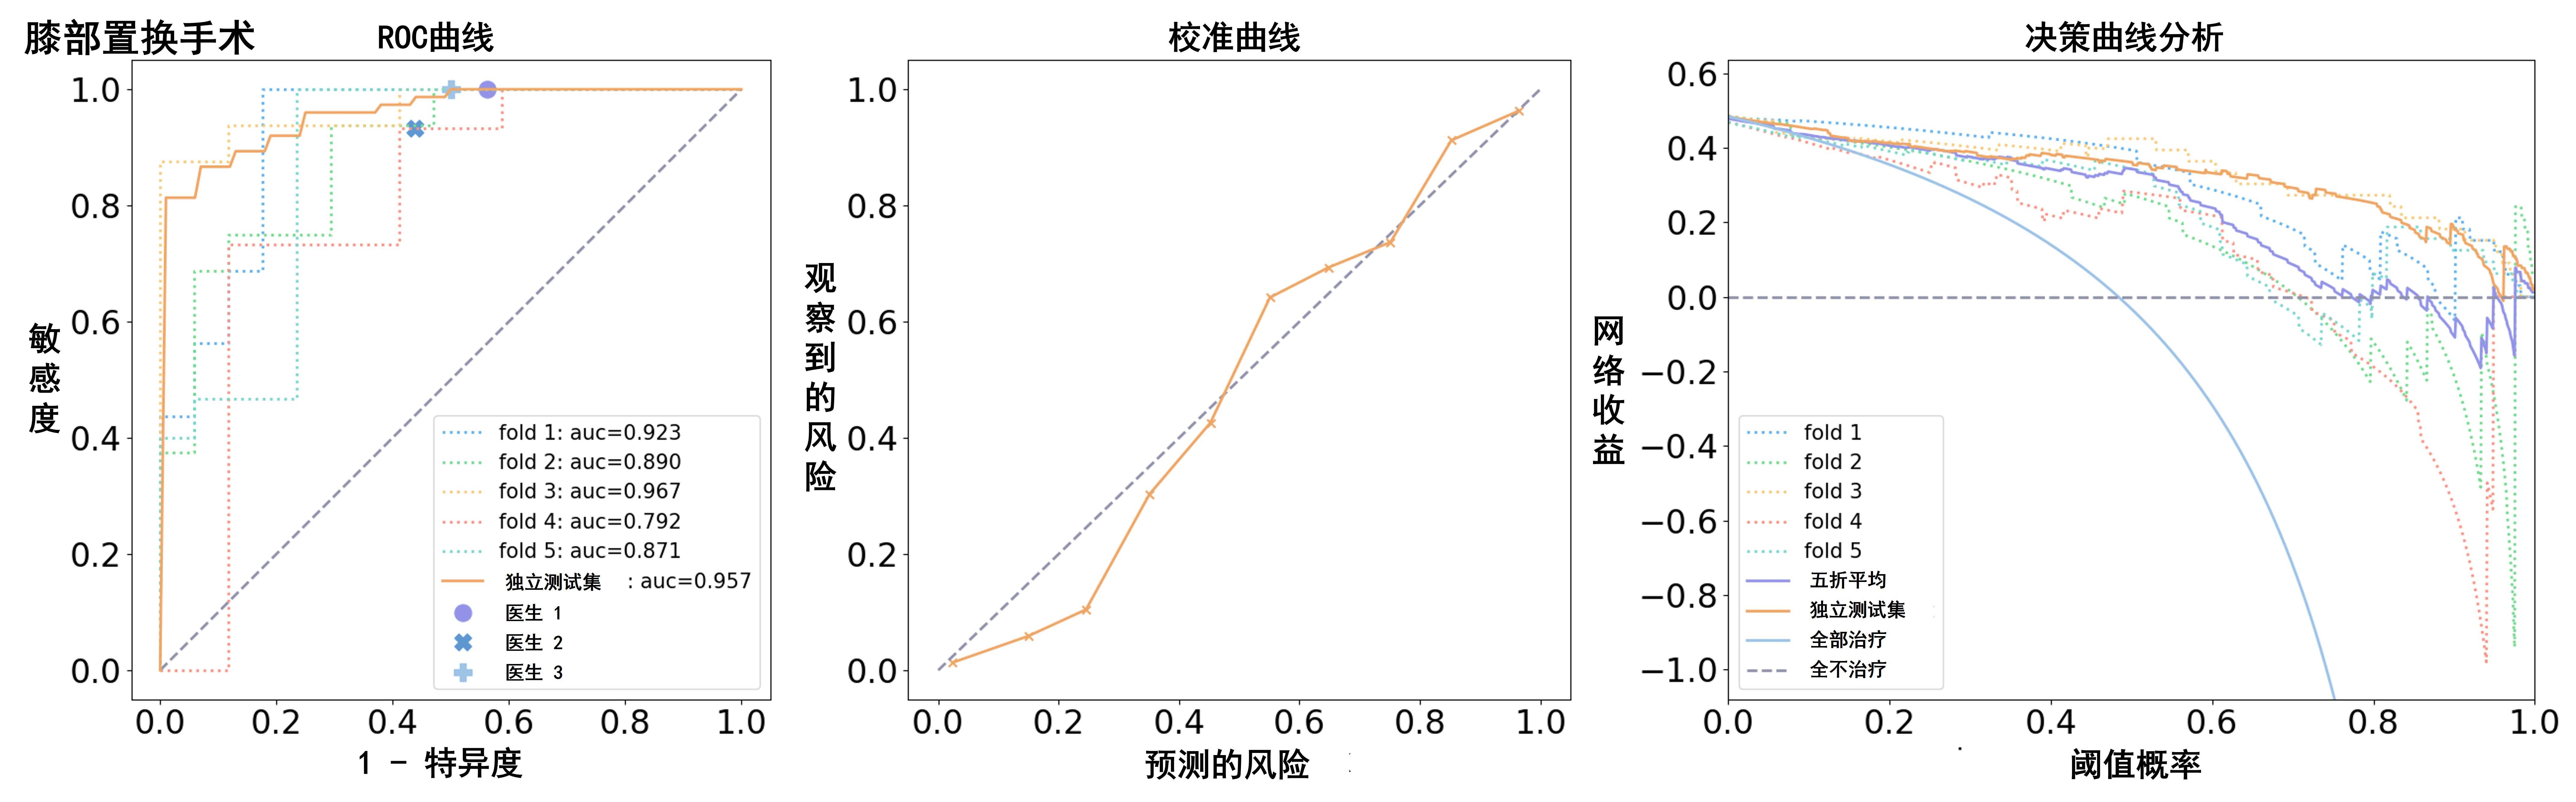
\includegraphics[width=\textwidth]{figures/chap03_curve_knee.jpg}
  }
  \newline
  \subfloat{
    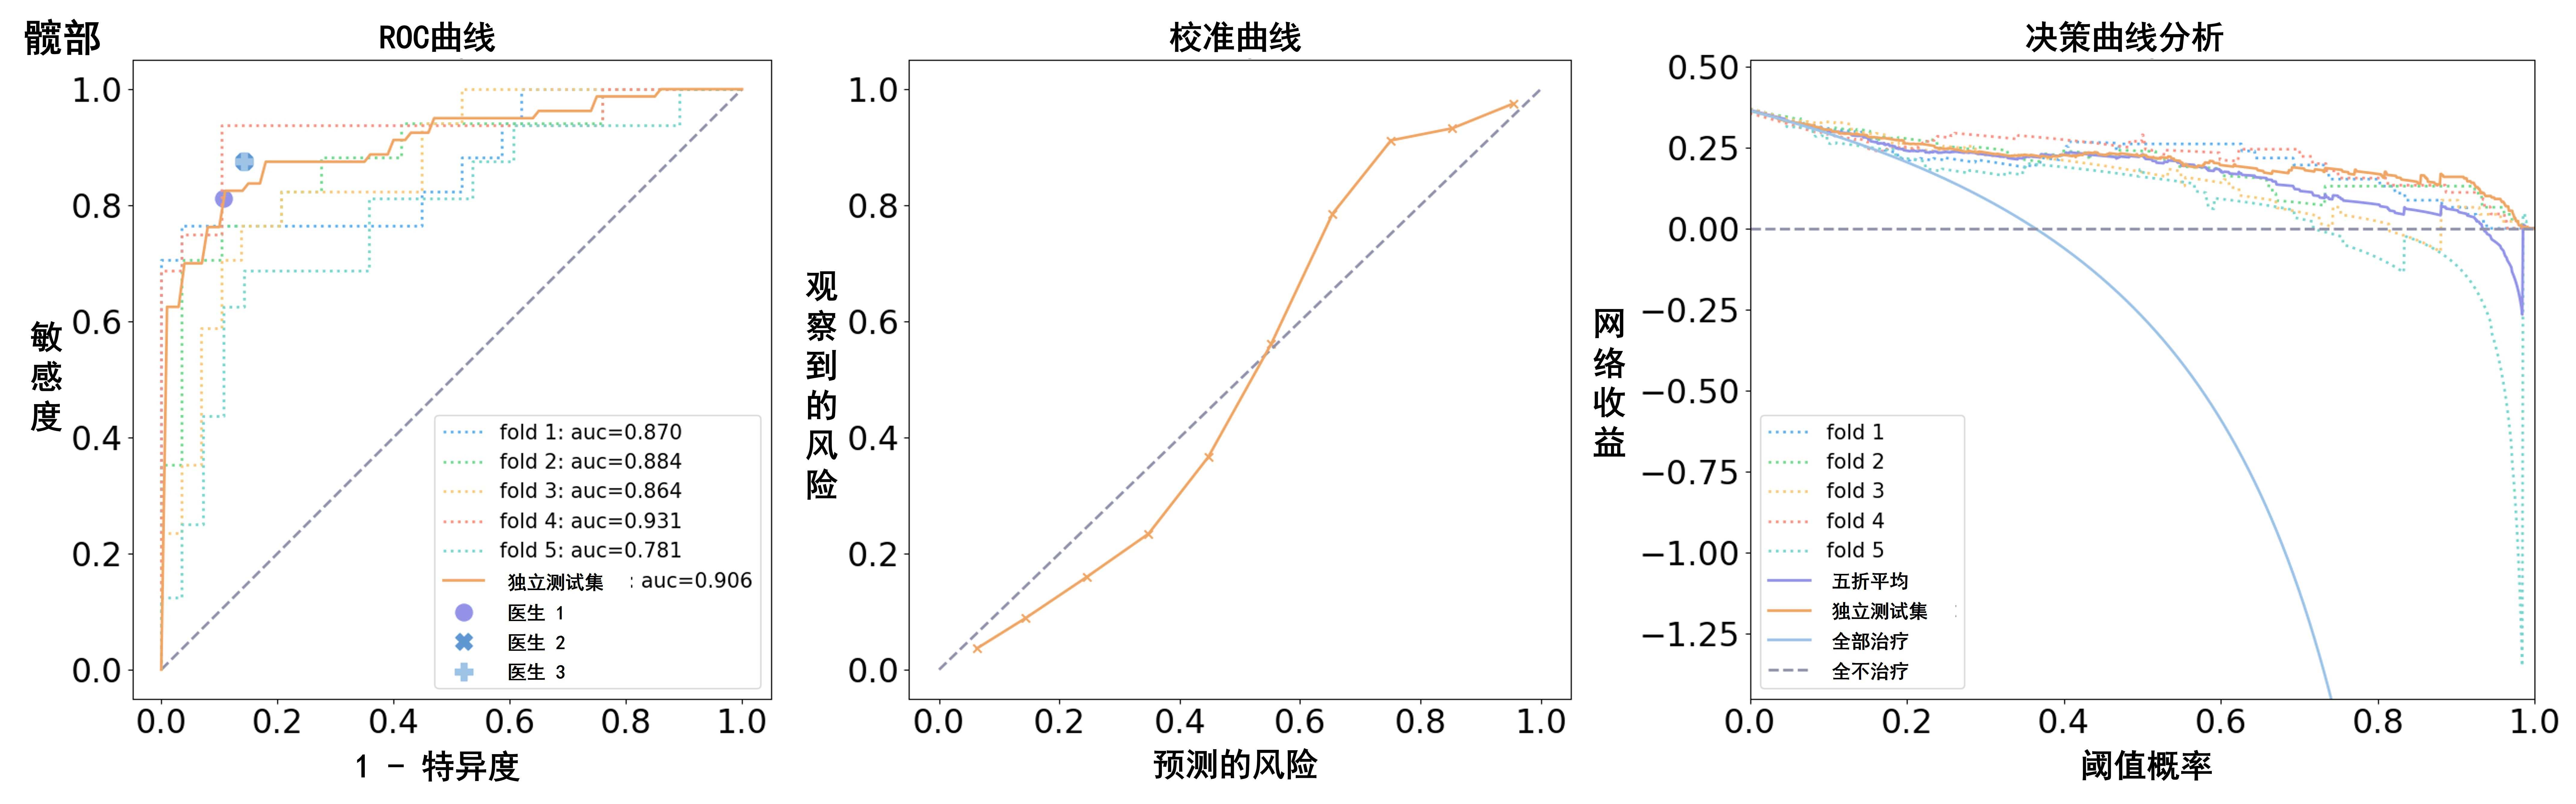
\includegraphics[width=\textwidth]{figures/chap03_curve_hip.jpg}
  }
  \caption{本章框架的ROC曲线(包含三名专业医生)、校准曲线与决策曲线分析}
  \label{fig:chap03_ROC_CC_DAC}
\end{figure}

图\ref{fig:chap03_ROC_CC_DAC}分别展示了本章框架在膝关节置换手术和髋关节置换手术动态骨显像数据集的ROC曲线、校准曲线与决策曲线分析。ROC曲线展示了展示了本章框架与三名专家相当的分类性能。其次,本章提出的框架的校准曲线较为贴近45度对角线,这反映了在膝关节置换手术和髋关节置换手术的动态骨显像数据集上假体关节感染的预测概率与假体关节感染的真实概率具有良好的一致性。此外,本章提出的框架在独立测试集上的决策曲线分析表明,假体关节感染的预测在所有阈值概率下拥有一个较高的净收益,而在五折交叉验证中,存在一到两折在高概率阈值下为负的网络净收益的情况。因此,在大多数情况下,在临床实践中是有价值且有益的。



\subsection{可视化分析}

动态骨显像与Grad-CAM获得的热力图融合后的图像如图\ref{fig:chap03_Grad-CAM_t-SNE}(a)所示。动态骨显像中血流相和血池相的病灶区域都是重要性最大的区域,这表明DBS-eNet在预测这些影像的最终结果时可以正确聚焦病灶区域,也验证了本章提出的方法符合核医学医生在诊断决策中的判断。

在图\ref{fig:chap03_Grad-CAM_t-SNE}(b)中,t-SNE得到的感染样本和未感染样本的特征点在膝关节置换手术和髋部关节置换手术数据集中都大致地被划分为两簇,体现了DBS-eNet提取的特征本身具有较好的可区分性,表明了该框架的良好性能。通过Grad-CAM和t-SNE方法,可以增加本章提出的框架的可解释性。此外,在对经历了关节置换手术的患者进行诊断时,如果医生之间的判定结果一致性较低,通过可视化框架的决策过程以及总结模型学习到的特定模式和影像学特征,可以为医生提供额外的意见作为参考,不仅有助于提高疾病诊断的准确率和效率,同时为后续的治疗和预后提供了有力的信息支持。

\begin{figure}[htbp]
  \centering
  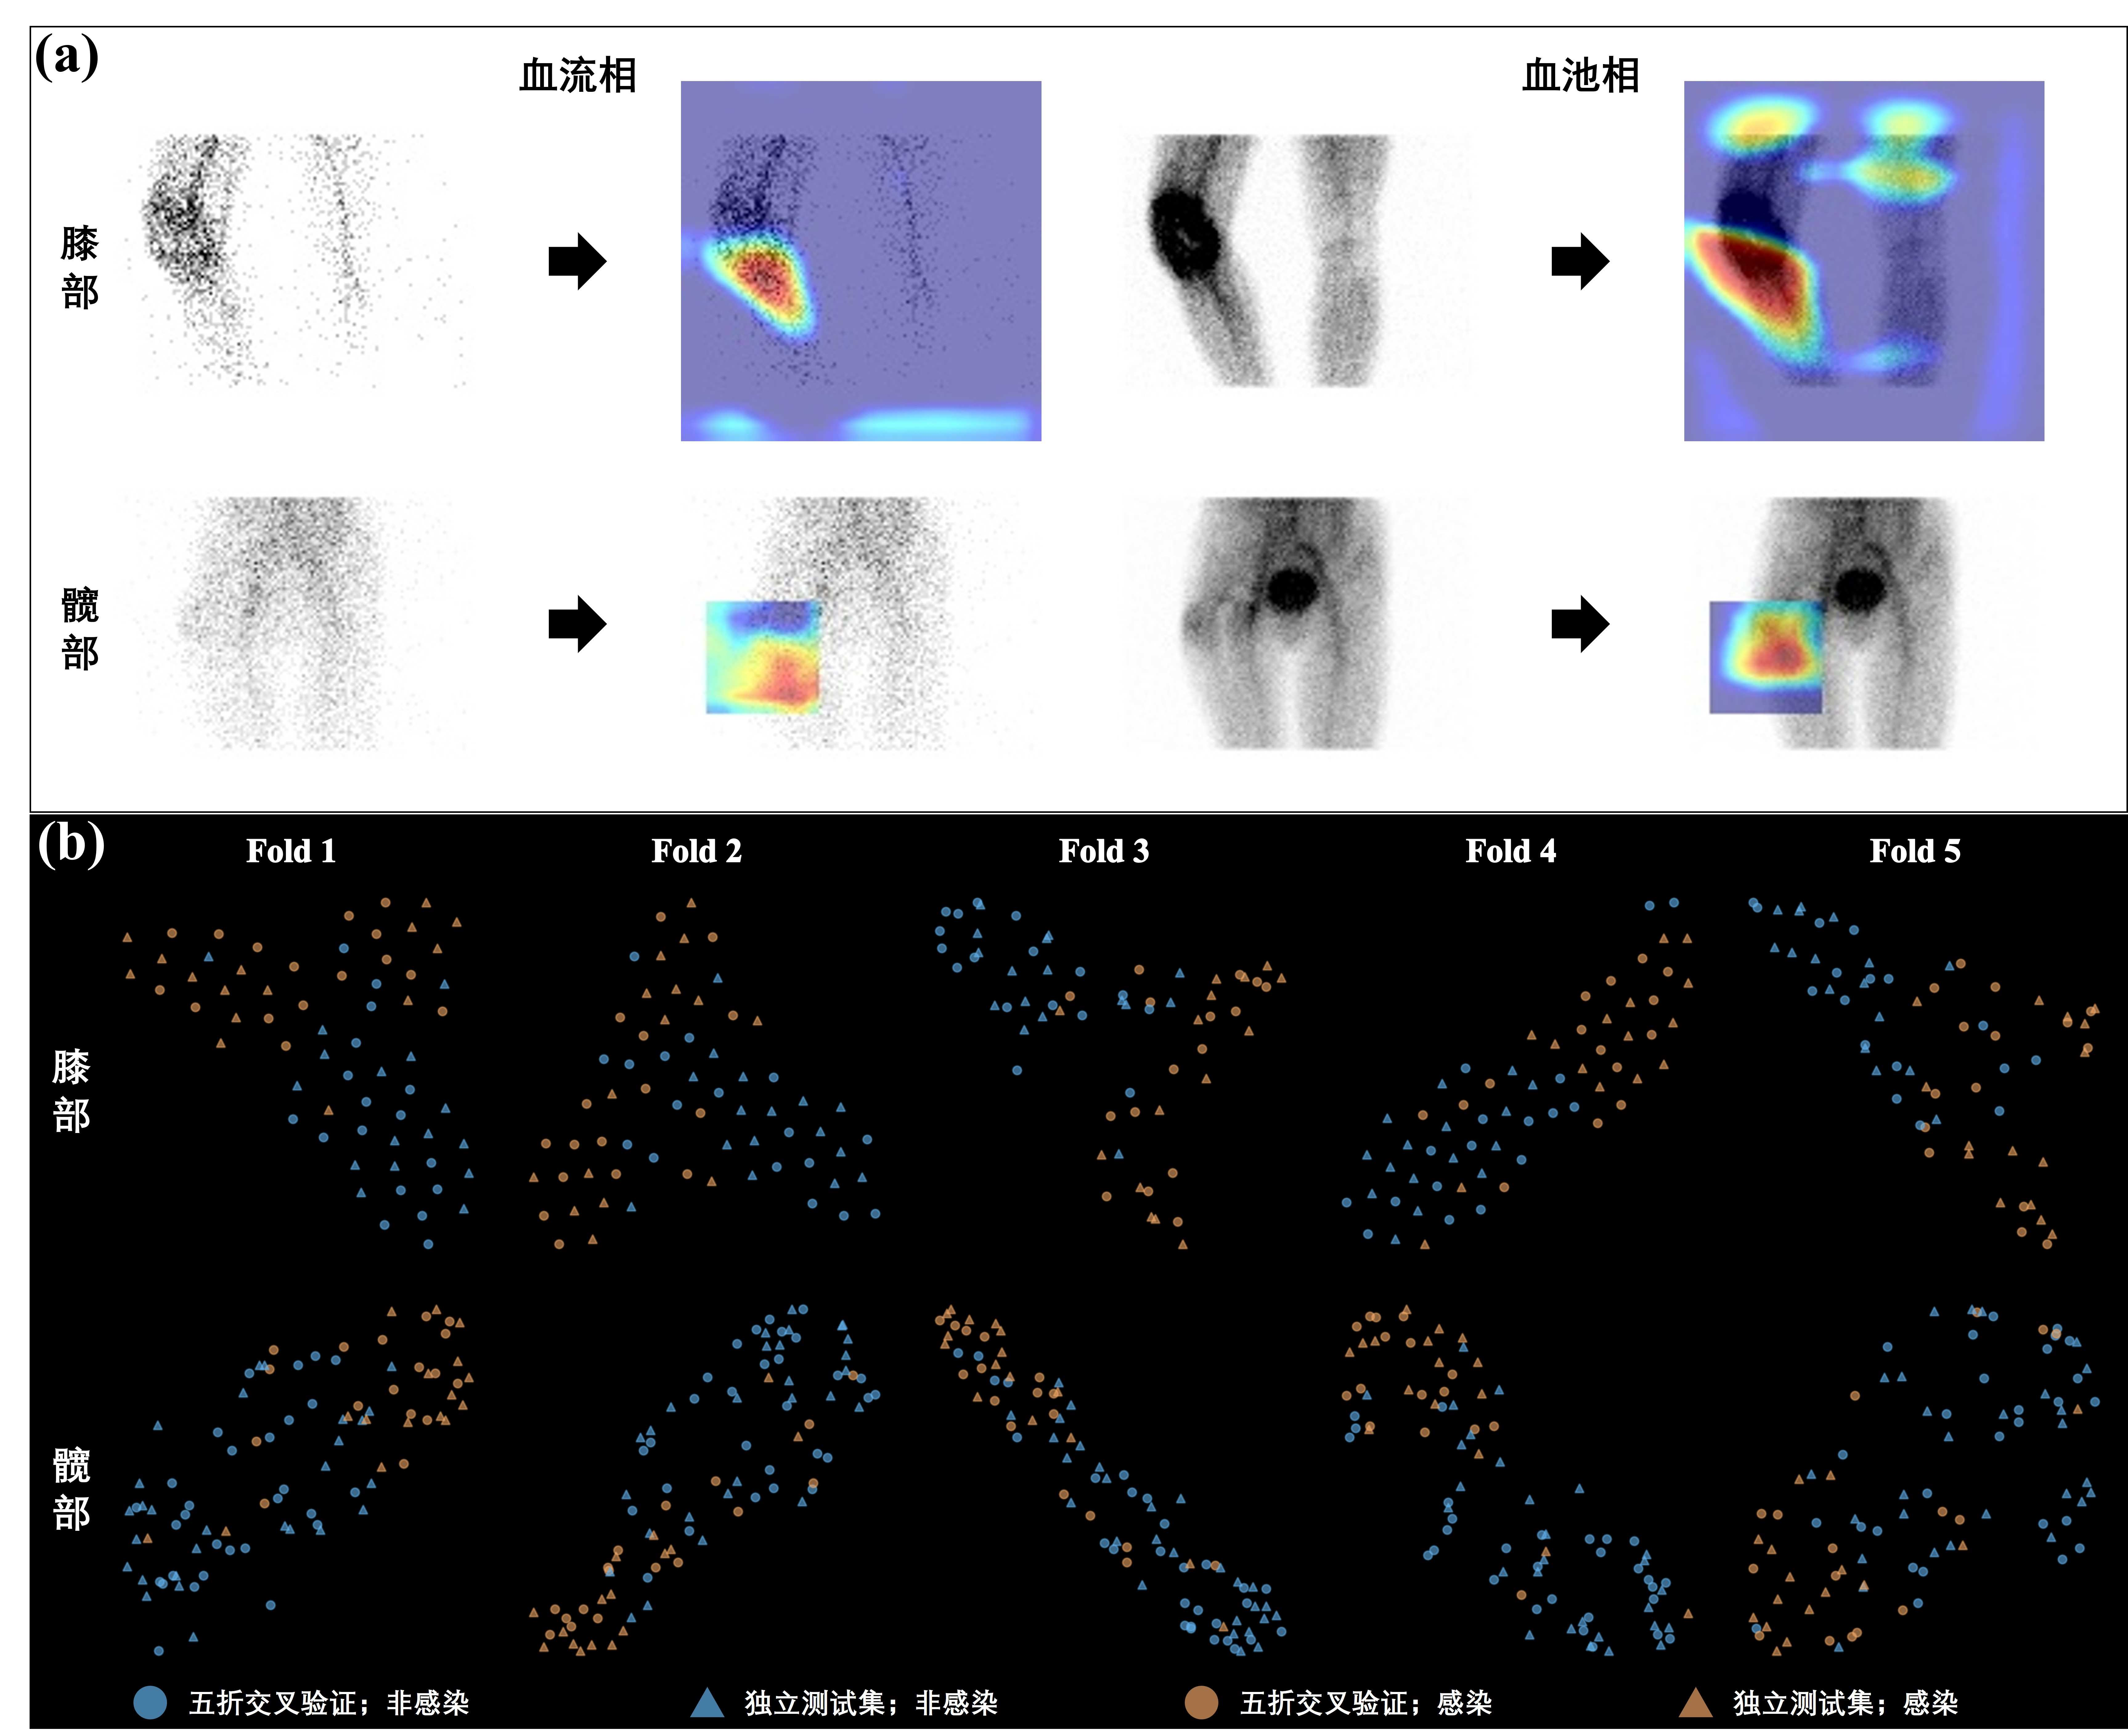
\includegraphics[width=\textwidth]{figures/chap03_Grad-CAM_t-SNE.jpg}
  \caption{(\textbf{a}) DBS-eNet的Grad-CAM热力图\quad(\textbf{b}) DBS-eNet的t-SNE散点图}
  \label{fig:chap03_Grad-CAM_t-SNE}
\end{figure}

\section{本章小结}

本章主要提出了一个基于\(^{99m}\)Tc-MDP动态骨显像的假体关节感染诊断框架。该框架包含了获取强度特征的标准预处理、获取差异特征的基于感兴趣区域预处理和用来提取生理摄取特征和时序性差异变化特征的DBS-eNet。实验结果表明,在综合性能表现上,该框架在膝关节上达到了86.48\% (80.98\%, 91.41\%)的准确率和0.889 (0.825, 0.933)的AUC,在髋关节上达到了86.33\% (81.50\%, 90.75\%)的准确率和0.866 (0.809, 0.911)的AUC,优于其他卷积神经网络。在与核医学专家的比较中,该框架的性能在诊断假体膝关节感染上优于专家,在诊断髋关节感染上与专家相当。这揭示了人工智能方法在诊断假体关节感染的可行性和诊断框架的有效性。在可视化结果中,该框架在动态骨显像上关注区域与专家相似,并且提出的特征具有明显的可区分性。这表明它可以有效辅助医生进行诊断决策,提升诊断质量。
% !Mode:: "TeX:UTF-8"
\chapter{基于\texorpdfstring{\(^{18}\)}{18}F-FDG PET/CT三维影像的下肢骨折相关感染检测与诊断框架}

上一章介绍了应用于骨三相中进行骨科相关感染诊断的人工智能方法,本章将根据PET/CT影像中骨科相关感染的诊断流程,研究患者下肢的骨折相关感染(Fraction-Related Infection)的检测与诊断,并提出了全自动两阶段的下肢骨折相关感染检测与诊断框架。第一阶段通过双分支三维定位网络检测病灶区域,第二阶段通过卷积神经网络进一步地进行病灶分类,预测是否存在感染。检测部分通过PET主分支和CT辅分支的网络结构设计有效地提取两种不同模态的特征并进行逐阶段地充分融合生理代谢信息和解剖组织信息。诊断分类部分对检测的病灶进行最大强度投影转换为二维影像,在降低数据和模型规模的同时保留有效特征,通过分类器计算得到预测结果。该方法可以较为准确地检测出病灶并拥有较高的诊断分类准确率。

\section{问题分析}


在应对PET/CT三维影像中下肢骨折相关感染的诊断任务时,需综合考虑医生对于骨折相关感染的诊断流程、PET/CT影像的特性,以及人工智能在该诊断任务中的应用可能面临的挑战,可以概括如下:

(1)\textbf{缺乏关于下肢骨折相关感染的公开数据集}。目前网络上暂无公开的关于骨折相关感染的数据集。由此,本文作者与上海市第六人民医院核医学科医生合作收集了来源于真实患者下肢的PET/CT影像,并构建了与真实分布一致的下肢骨折相关感染的PET/CT影像多模态数据集。然而,数据集整体规模相对较小,而且在类别上分布不平衡。\textbf{这种数据集的特性对于模型的训练提出了额外的挑战}。

(2)\textbf{CT中骨折相关感染病灶的形状与分布区域多样}。在骨折相关感染的临床诊断流程中,首要任务是明确病变的具体位置。尽管骨折相关感染的病灶位置与骨骼强度相关,但由于人体骨骼广泛分布于全身,与一些组织和器官相比,并不像它们存在于一个相对固定的位置或者范围内。其次,病变的程度也有所差异,可能会涉及骨骼的不同部位以及软组织的破裂和损伤,也可能因个体差异而不同,导致病灶形状多变。因此,\textbf{对于骨折相关感染的病灶位置,是否能够准确地检测出至关重要}。

(3)\textbf{PET中高摄取区域呈现的形式和程度各不相同}。从核医学影像的角度分析,PET影像可以通过人体的组织细胞对于示踪剂氟代脱氧葡萄糖的摄取程度来展示人体的生理代谢信息。生理代谢强的区域一般都有着对于示踪剂的摄取程度高的特点,但呈现的形式与程度也各不相同。此外,人体中存在的自然高摄取区域(膀胱、肾脏等),以及炎症和愈合过程都会导致周围的软组织的摄取能力增加。骨折相关感染的病灶区域也因自身病变程度的不同而展示出各种不同的摄取形式和程度。因此,\textbf{如何避免其他高摄取区域造成的混淆是一个本章研究的主要问题}。

(4)\textbf{PET和CT影像之间不同的特征}。PET和CT是两种不同的医学影像模态,各自可以表现不同的内容信息。PET影像可以展现出人体的生理代谢信息,而CT影像可以展现出人体的解剖组织信息。同时,PET和CT均为三维影像。因此,\textbf{充分利用PET和CT影像的两种不同信息以及它们本身的三维性质同样是一个值得研究的问题}。

(5)\textbf{病灶检测中正负样本不平衡}。在本章的下肢骨折相关感染数据集中,一个病人一般仅有一个或二个病灶。对于病灶检测任务而言,所需要检测的目标数量少,会导致影像中的正负样本数量差异巨大,这将是一个\textbf{严重的正负样本不平衡问题}。此外,目前的检测方法中,有基于先验框的方法,也有不基于先验框的方法。\textbf{哪种方法更加适用于本章的研究方法也是值得去考虑的问题}。

根据上述的几个问题,本章提出了两阶段的下肢骨折相关感染的检测诊断方法,该方法主要从以下几个方面进行针对性地研究:

(1)针对数据集的问题,本章设计了\textbf{一套针对于PET/CT影像的数据预处理方法}(PET/CT配准、去除机床等无关区域),以及其中的适应性修改的数据增强方法(翻转、Mixup\cite{zhang2017mixup}和RICAP\cite{takahashi2018ricap})能够极大地增加数据集的多样性,缓解数据集较小的问题。经过这样一整套预处理流程的PET/CT影像可以去除掉较大的无关区域,有效地提升模型的性能和预测结果。

(2)针对骨折相关感染病灶难以准确检出的问题,\textbf{设计了一个并行双分支的病灶定位三维网络模型}。通过主干网络的并行双分支设计,加强对PET和CT影像特征的提取和结合能力,有效地学习病灶在生理代谢中摄取能力较高、呈点状或弥漫性的特点,以及在解剖组织中骨骼部位存在缺失、断裂或金属植入物的特点,将丰富的语义信息提供给后续的特征融合子网和预测子网。

(3)针对高摄取区域之间易产生混淆的问题,本章\textbf{添加自然高摄取区域的标注,并且通过CT影像的补充和注意力机制来排除其他情况带来的干扰}。由于自然高摄取区域(膀胱)的位置相对固定的特点,相比于病灶区域,更容易让定位网络自主学习到,进而能够有效地减少自然高摄取区域的干扰。此外,通过CT影像的补充以及注意力机制,更好地排除掉与骨骼不相关的高摄取区域,进而促进定位性能的提升。

(4)\textbf{PET和CT影像之间的特征相互补充和相互促进}驱使本章引入并行双分支病灶定位网络。其次,考虑到PET/CT影像的三维性质,定位网络中的二维计算方式都调整为相应的三维计算方式。这样的调整适用于三维影像的结构,以更全面地捕捉影像的立体信息,更准确地学习病灶在深度方向上的分布和形态,从而提高网络对于骨折相关感染任务中的立体病灶的处理效果。

(5)对于正负样本不平衡的问题,本章研究通过\textbf{多方面的改进策略}进行优化。首先,引入了新的检测目标;其次,在训练过程中,采用了SimOTA标签匹配策略,以实现对正样本数量的动态匹配;最后,在病灶定位网络的特征融合网络和预测网络中进行了修剪设计,以缓解正负样本极端不平衡的问题。此外,先验框可以通过人工设计或者在数据集中采用聚类方法生成,人工设计难度较大,而采用聚类方法,在本章研究中存在数据集较小的问题,可能会导致生成的先验框存在一定的偏差,因此,本章研究采用无先验框的目标检测方法。

\begin{figure}[htbp]
  \centering
  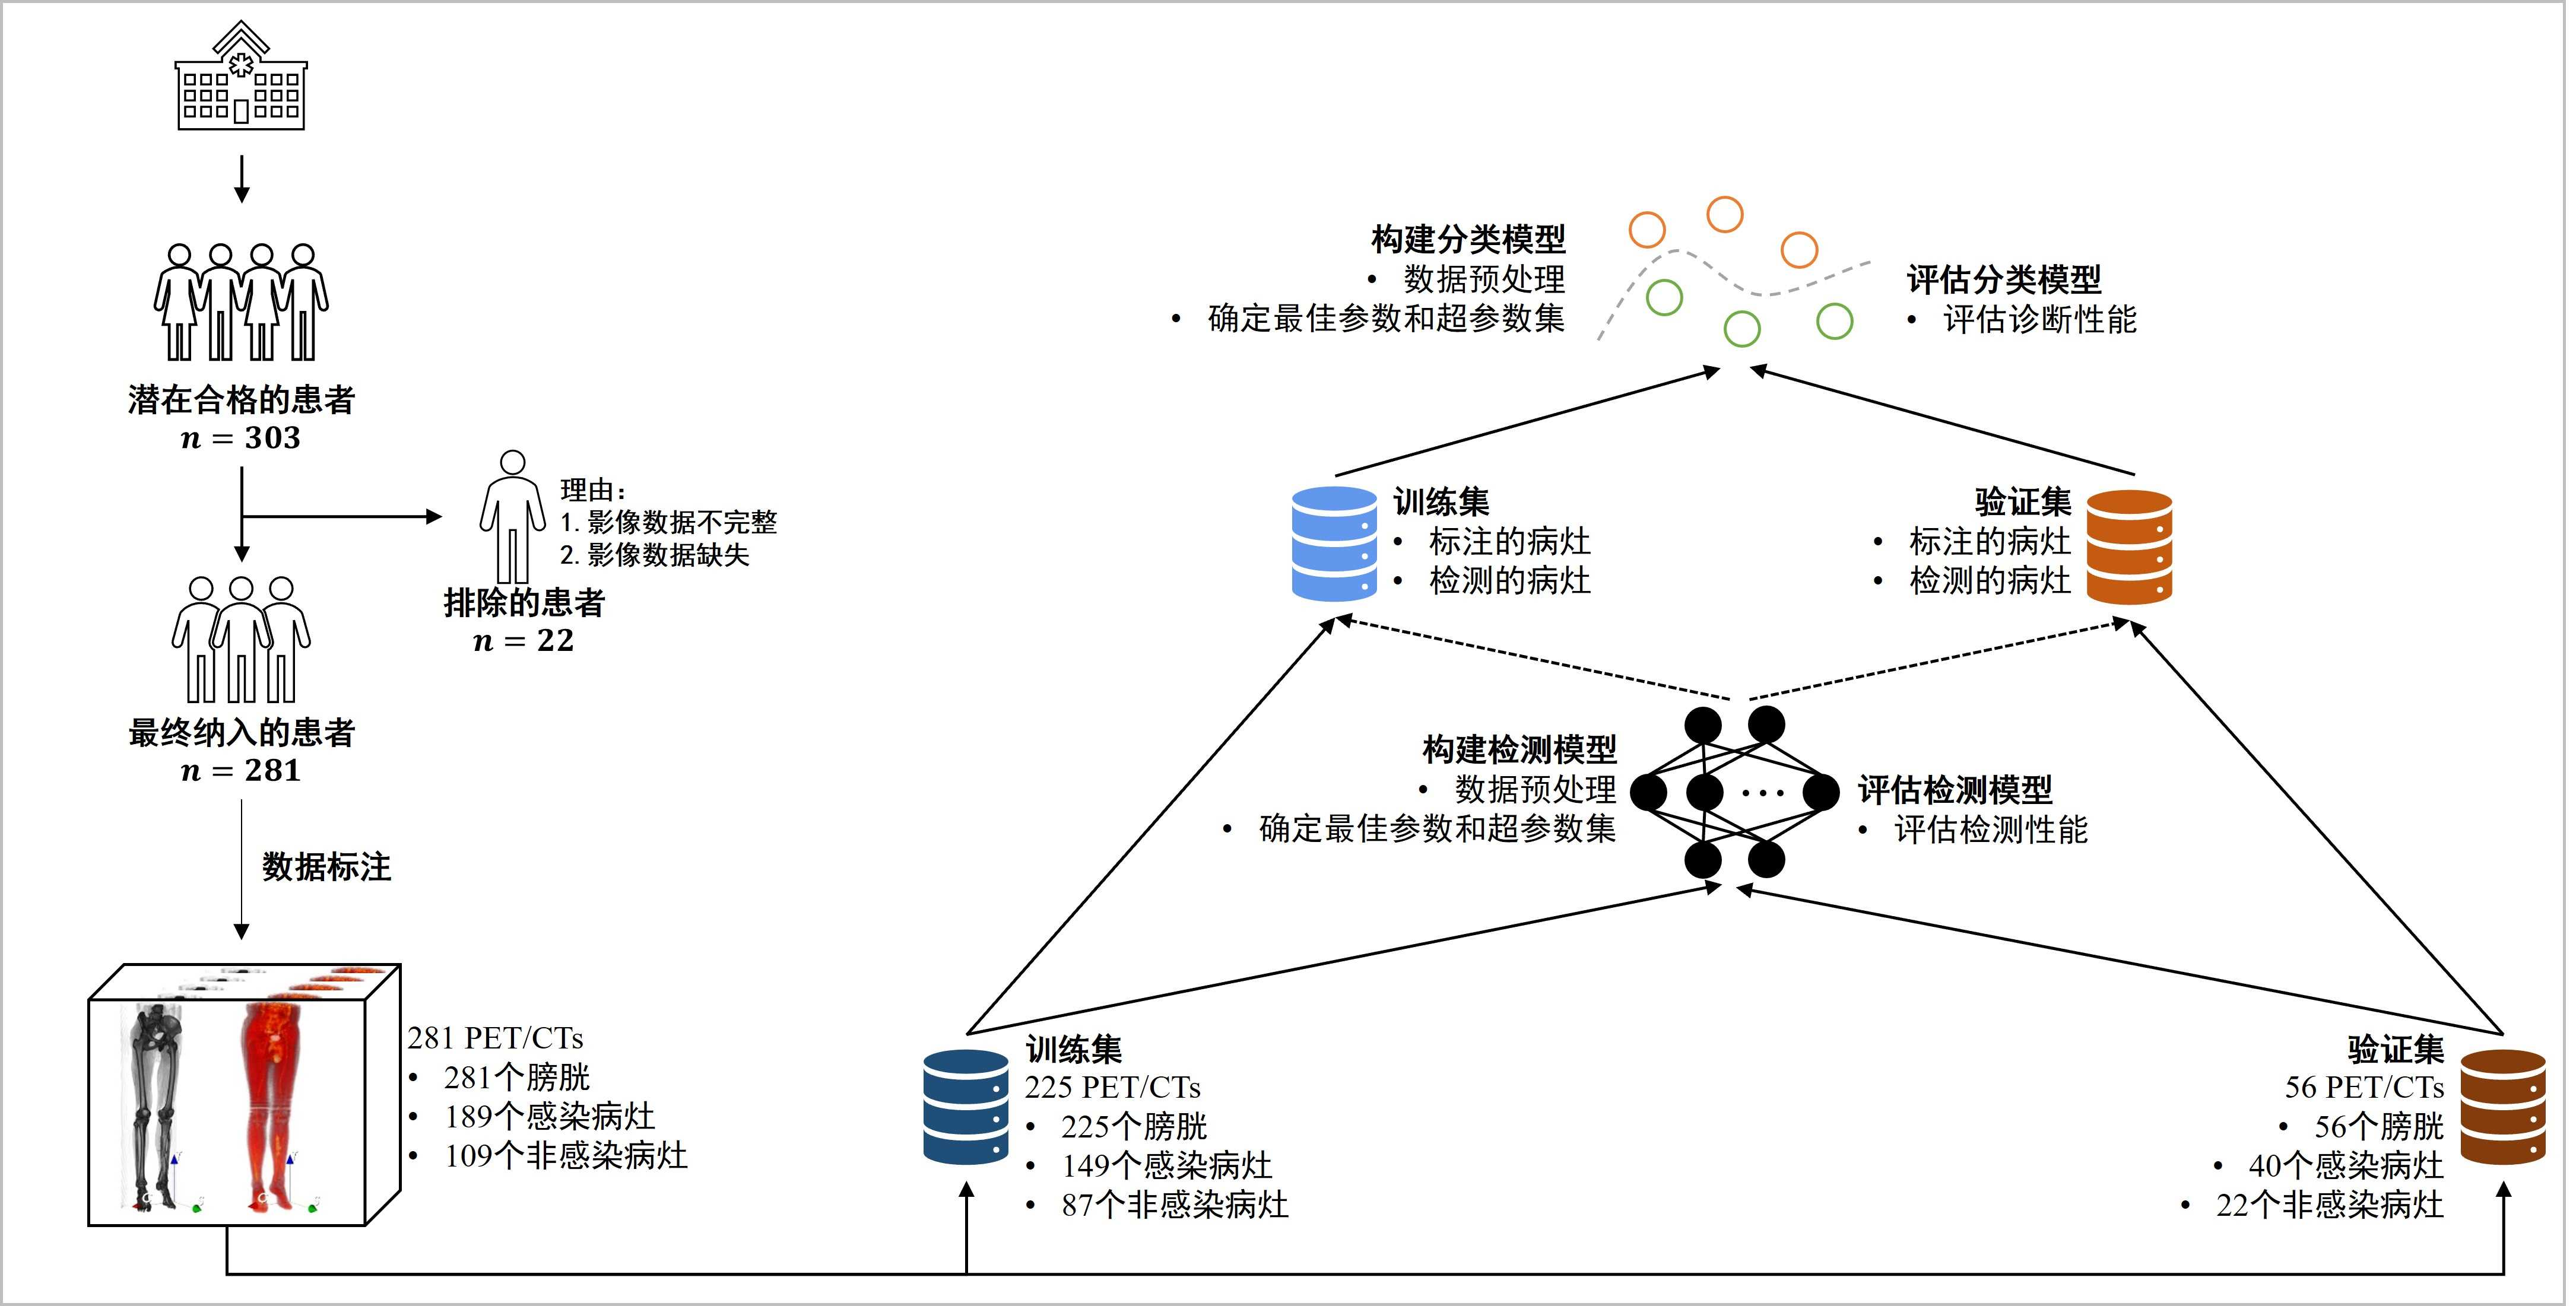
\includegraphics[width=\textwidth]{figures/chap04_study.jpg}
  \caption{本章研究的整体流程}
  \label{fig:chap04_study}
\end{figure}

本章研究的整体流程如图\ref{fig:chap04_study}所示。首先,通过最初的数据收集、筛选与标注,最终得到了包含了281名患者的PET/CT影像数据。其中,有281个膀胱标注、180个感染病灶标注和109个非感染病灶标注。其次,按照4:1的患者个体数量比例进行划分,得到了包含了225个患者PETCT影像数据的训练集(膀胱、感染病灶与非感染病灶:225 vs. 149 vs. 87)和包含了56个患者PETCT影像数据的验证集(膀胱、感染病灶与非感染病灶:56 vs. 40 vs. 22)。随后,设计和构建第一阶段的检测模型。通过使用训练集的训练结果,适应性地调整模型结构、超参数和训练策略,并利用验证集来进一步评估该模型的检测性能,获得最终的检测模型和最佳超参数。最后,设计和构建第二阶段的分类模型。利用第一阶段中检测模型在训练集和验证集中的检测结果添加到第二阶段的训练集和验证集中来扩充数据集的规模。同样地使用训练集的训练结果来适应性地调整模型、超参数和训练策略,并利用验证集来进一步评估该模型的分类性能,获得最终的分类模型和最佳超参数。最终二阶段的框架包含了最佳的检测模型和最佳的分类模型组成。

\section{数据预处理}

针对PET/CT影像中骨折相关感染的检测诊断任务,本章提出了一套完整的PET/CT影像的预处理算法,其具体流程如下:

(1)数据清洗与标注:清洗收集的患者PET/CT影像数据并进行三维目标框及其类别标注;

(2)PET/CT的转换与配准:首先,将CT影像中的像素值转换为用于测量组织对X射线的衰减程度的亨氏单位(Hounsfield Unit,HU),并且将PET影像中的像素值转换为用于半量化分析生理代谢活动的标准摄取值(Standardized Uptake Value, SUV)。然后,由于PET与CT影像的采样分辨率不一致,因此通过配准将PET和CT影像在物理空间中的原点、体素间距、尺寸大小变成一致。

(3)人体区域保留:考虑到PET/CT影像中非人体区域所占空间较大,并且机床属于纯粹的无关干扰区域,因此可彻底剔除该部分以提高影像质量和解剖学解析度。

(4)数据增强:通过翻转、适应性修改的Mixup和RICAP(Random Image Cropping And Patching)增加PET/CT影像中的检测目标数量,并扩充数据集的规模。

\subsection{数据清洗与标注}

\begin{figure}[htbp]
  \centering
  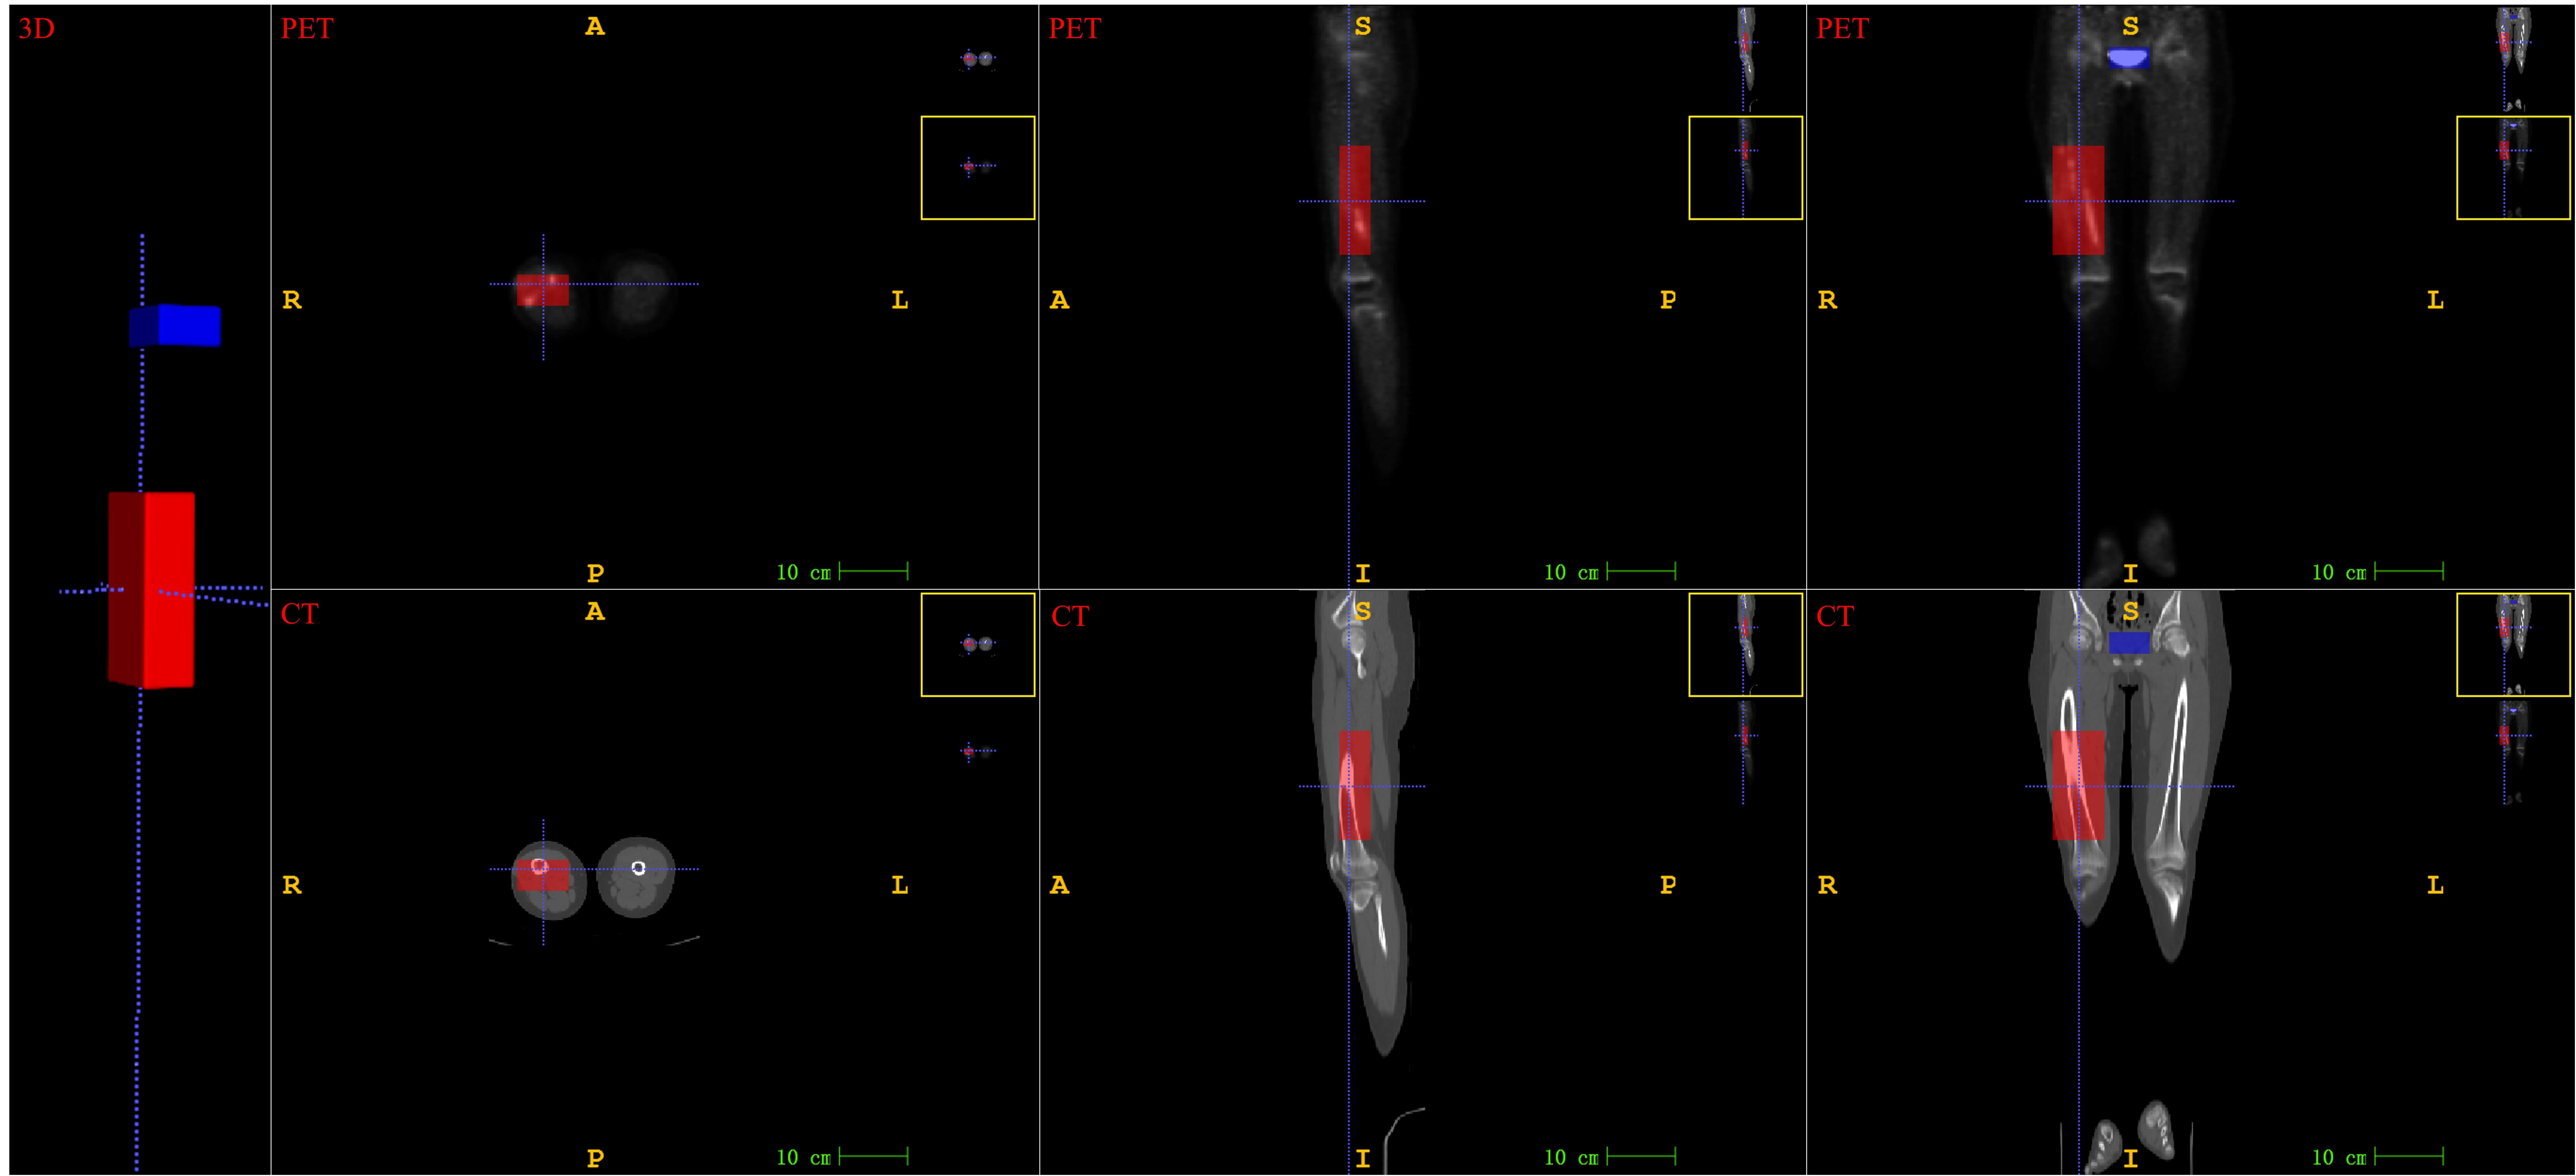
\includegraphics[width=\textwidth]{figures/chap04_label.jpg}
  \caption{PET/CT影像的数据标注}
  \label{fig:chap04_label}
\end{figure}

本章所采集的PET/CT影像数据同样是以DICOM格式存储。首先,对收集到的PET/CT影像数据进行清洗,例如排除掉不完整或存在缺失的影像数据。此外,为了保护病人的个人隐私信息,对DICOM格式文件进行脱敏,去除掉DICOM格式文件中有关于病人、医院、医生、设备制造商等等所有隐私数据。在经过上述操作后,本文作者在专业的核医学医生的指导下使用ITK-SNAP软件(v3.8.0, http://www.itksnap.org)对所有患者的PET/CT影像进行标注。最终标注结果由专业医学进行了核查。标注根据患者诊断报告为依据,在每一个患者的PET/CT影像上采用不同的颜色标注膀胱、感染病灶和非感染病灶,如图\ref{fig:chap04_label}所示。

\subsection{PET/CT的转换与配准}

HU是由CT扫描仪测量的组织相对于水的相对线性密度值。它提供了一种标定和对比度一致的方法,使得不同的CT扫描仪和不同扫描参数下的图像能够具有相似的密度值。此外,不同类型的组织对X射线具有不同的吸收能力,它们在CT中会展示出不同的亮度。将这些亮度转换为HU可以更加直观地表示组织的相对密度值,有助于区分不同的组织,也更方便于医生与研究人员进行更精确的定量分析。由此,本章将以DICOM格式存储的CT影像的像素值转换为HU值。

读取CT的DICOM文件,提取该文件中所需要的元数据:标签为(7FE0,0010)且关键字为像素数据(Pixel Data)的像素值\(P_{ct}\)、标签为(0028,1052)且关键字为重缩放截断值(Rescale Intercept)的截距\(b\)和标签为(0028,1053)且关键字为重缩放斜率(Rescale Slope)的斜率\(m\)。最后,通过公式\ref{eq:chap04_hu}转换为HU值。
\begin{equation}
  HU = m \times P_{ct} + b
  \label{eq:chap04_hu}
\end{equation}

SUV是一种用于衡量PET图像中肿瘤摄取的相对标准单位,通常用于定量分析和治疗反馈。SUV可以减少多种因素带来的影响,如患者的体重、注射剂量、扫描设备的差异、扫描时间、重建算法等等,使得不同患者、不同设备和不同扫描时期的PET影像结果具有可比性。此外,SUV值可以用于临床评估和治疗反馈,通过衡量肿瘤对放射性标记物的摄取程度,有助于评估肿瘤的活性、生物学特性以及治疗效果。由此,本文将以DICOM格式存储的PET影像的像素值转换为SUV值。

\begin{figure}[b]
  \centering
  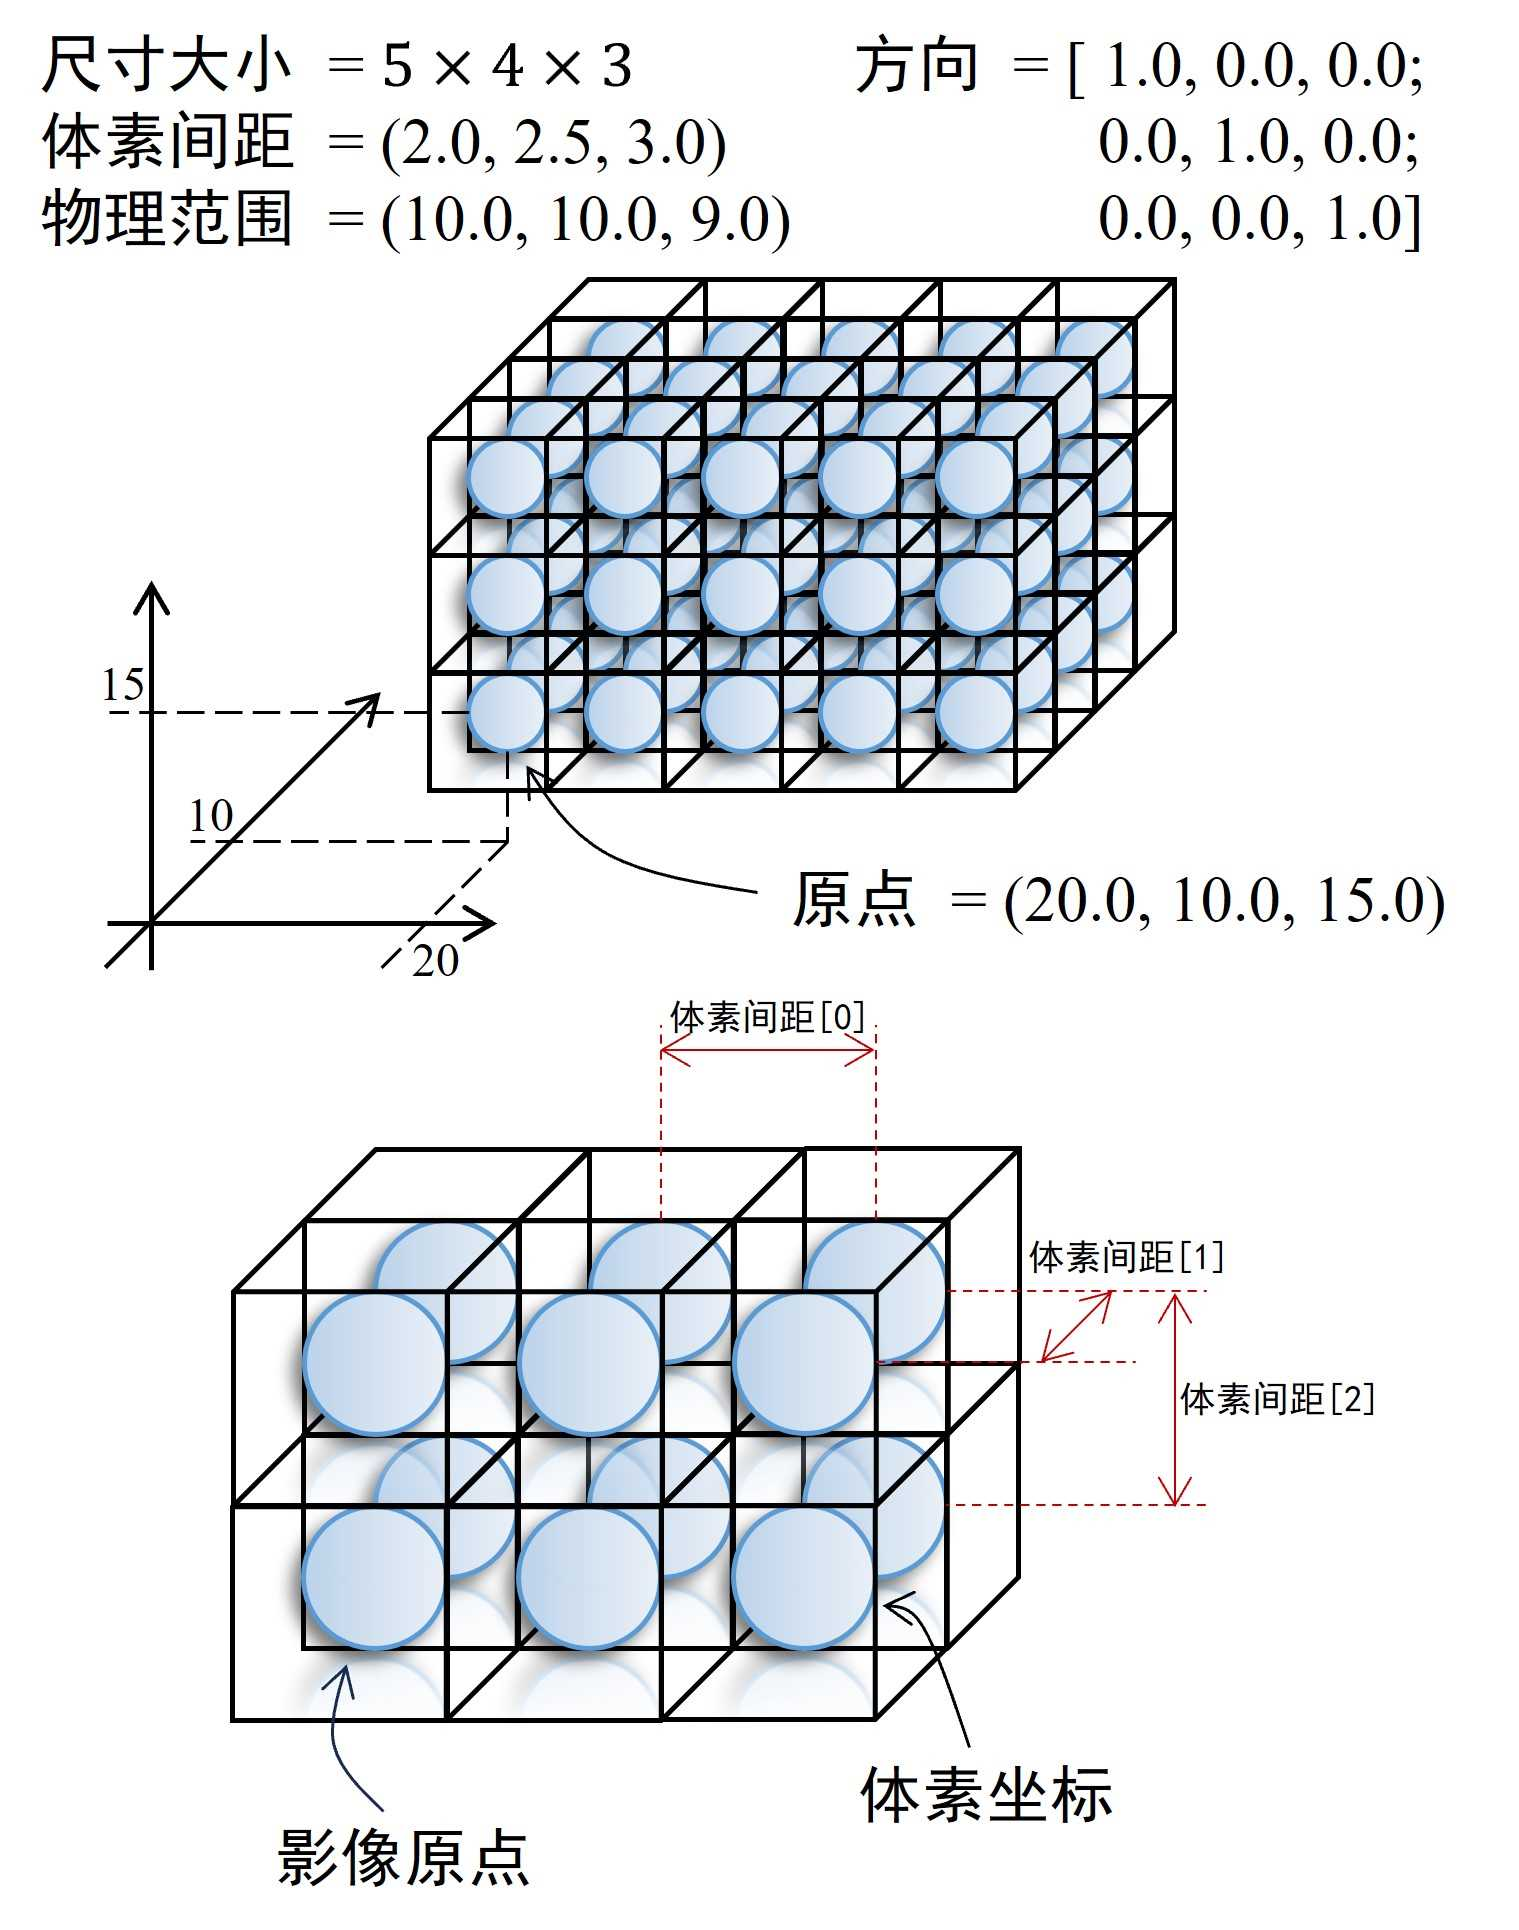
\includegraphics{figures/chap04_image.jpg}
  \caption{PET和CT影像在物理空间中所占据的区域}
  \label{fig:chap04_image}
\end{figure}

读取PET的DICOM文件。首先提取标签为(0010,1030)且关键字为病人体重(Patient Weight)的体重\(w\),计算病人的体重指标\(\mathcal{BW}\):
\begin{equation}
  \mathcal{BW} = 1000 \times w
\end{equation}
其次,提取标签为(0008,0021)且关键字为系列日期(Series Date)的扫描日期\(s_d\)、标签为(0008,0031)且关键字为系列时间(Series Time)的扫描时间\(s_t\)和标签为(0018,1072)且关键字为放射性药物开始时间(Radiopharmaceutical Start Time)的测量时间\(m_t\),来计算扫描到测量之间经过的时间\(\mathcal{T}\):
\begin{equation}
  \mathcal{T} = seconds(s_ds_t - s_dm_t)
\end{equation}
其中,\(seconds(\cdot, \cdot)\)表示计算两个时间戳之间的秒数。然后,提取标签为(0018,1074)且关键字为放射性核素总剂量(Radionuclide Total Dose)的注射剂量\(d\)和标签为(0018,1075)且关键字为放射性核半衰期计量(Radionuclide Half Life)的半衰期\(f\),来计算药物活性\(\mathcal{AC}\):
\begin{equation}
  \mathcal{AC} = d \times 2^{-\frac{\mathcal{T}}{f}}
\end{equation}
最后,提取标签为(7FE0,0010)且关键字为像素数据(Pixel Data)的像素值\(P_{pt}\)、标签为(0028,1052)且关键字为重缩放截断值(Rescale Intercept)的截距\(b\)和标签为(0028,1053)且关键字为重缩放斜率(Rescale Slope)的斜率\(m\),通过公式\ref{eq:chap04_suv}转换为SUV值。
\begin{equation}
  SUV = (m \times P_{pt} + b) \times \mathcal{BW} \div \mathcal{AC}
  \label{eq:chap04_suv}
\end{equation}

PET和CT是核医学影像中常见的两种三维模态影像。它们由一组点组成,每个点占据了空间中一部分物理区域。这与其他作为数组的图像之间存在着很大的差异,例如其他图像的像素或体素的间距是各向同性的,并且没有图像位置在物理空间的概念。如图\ref{fig:chap04_image}所示,PET和CT影像所占据的物理空间区域由影像的原点、间距、尺寸和方向余弦矩阵所确定。其中,原点是在每一维上的索引均为0的体素在世界坐标系上的位置;间距是每个维度上体素之间的间距;尺寸是每一个维度上体素的数量;方向余弦矩阵是每个轴的方向。

在本章收集的数据集中,PET和CT的原点、体素间距与尺寸大小都存在差异。因此,为了充分利用与融合PET和CT两种模态影像数据,本章采用了SimpleITK工具库\cite{yaniv2018simpleitk}进行配准。在经过前面处理计算得到的HU和SUV替换掉原来的像素值的基础上,使用SimpleITK中的函数Resample按照CT的原点、体素间距与尺寸大小对PET进行重采样。

\subsection{人体区域保留}

在对PET和CT进行转换和配准之后,由于PET和CT图像中含有过多与任务无关的区域以及CT中存在的扫描设备机床容易影响模型训练和检测性能。本章提出了一个人体区域保留算法,人体区域保留前后效果如图\ref{fig:chap04_body_retent}所示。人体区域保留算法流程如下:

\begin{figure}[htbp]
  \centering
  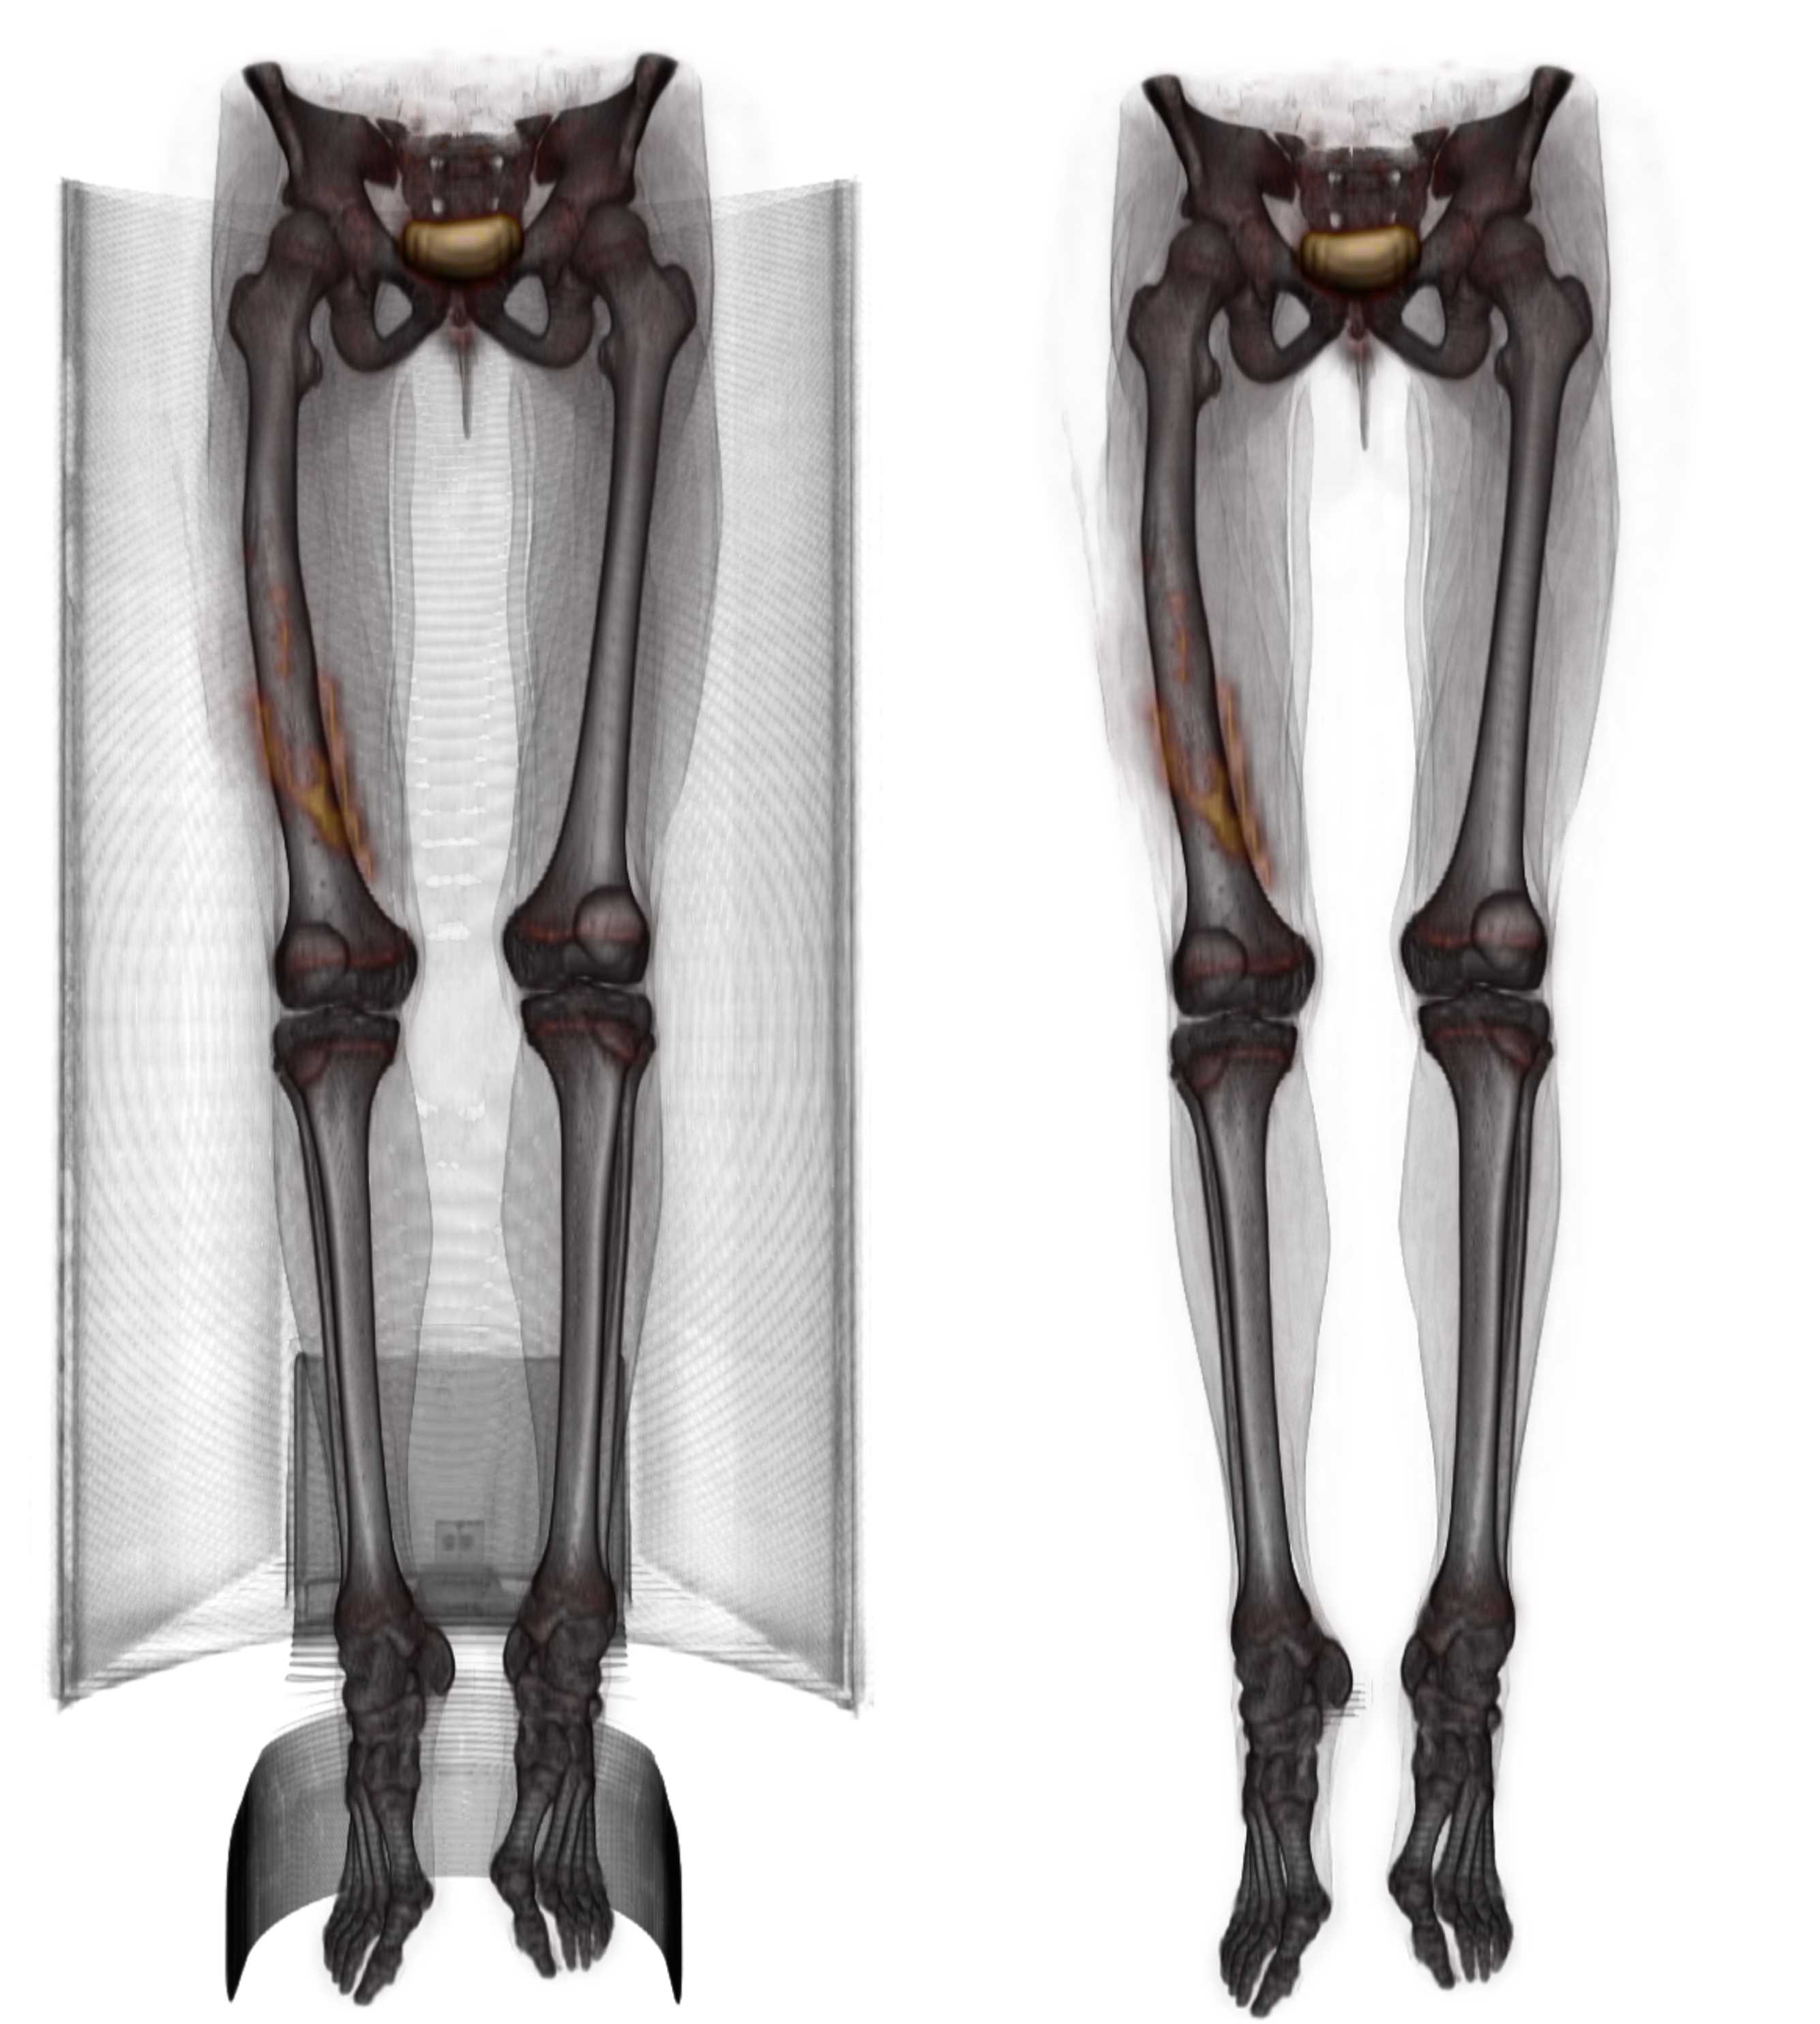
\includegraphics[width=0.8\textwidth]{figures/chap04_body_retent.jpg}
  \caption{人体区域保留算法前后对比}
  \label{fig:chap04_body_retent}
\end{figure}

(1)读取CT影像中的HU三维数组\(Arr_{HU}\)和PET影像中的SUV三维数组\(Arr_{SUV}\)。通过在CT和PET上分别进行图像二值化计算出初步的分割掩码图\(maskB_{HU}\)和\(maskB_{SUV}\),如公式\ref{eq:chap04_mask_binary}所示:
\begin{equation}
  \begin{aligned}
    maskB_{HU}^{i, j, k}  & =
    \begin{cases}
      1 , & \text{if \(Arr_{HU}^{i, j, k} > -200\)} \\
      0 , & \text{otherwise}
    \end{cases}  \\
    maskB_{SUV}^{i, j, k} & =
    \begin{cases}
      1 , & \text{if \(Arr_{SUV}^{i, j, k} > 0.001\)} \\
      0 , & \text{otherwise}
    \end{cases} \\
  \end{aligned}
  \label{eq:chap04_mask_binary}
\end{equation}
其中,\(i,j,k\)表示三个维度上的索引。

(2)使用一个核半径为2且形态为球形的图像滤波\(F_2\)对二值化得到的分割掩码图进行形态学闭操作,用以去除小孔,平滑边界,使得分割掩码图更加完整,如公式\ref{eq:chap04_mask_close}所示:
\begin{equation}
  \begin{aligned}
    maskB_{HU}  & = (maskB_{HU} \oplus F_2 ) \ominus F_2  \\
    maskB_{SUV} & = (maskB_{SUV} \oplus F_2 ) \ominus F_2
  \end{aligned}
  \label{eq:chap04_mask_close}
\end{equation}
其中,\(\oplus\)表示形态学上的膨胀操作,\(\ominus\)表示形态学上的腐蚀操作。

(3)计算分割掩码图\(maskB_{HU}\)和\(maskB_{SUV}\)的最大连通量。首先,扫描分割掩码图,对其中的每个连通区域标记一个唯一的标签\(L\)。然后,统计每一个标记区域的体素数量\(S\)。最后,选择具有最大体素数量的标记区域,即最大连通量:
\begin{equation}
  L_{max} = \mathop{\arg\max}_{i=1}^N S_i
\end{equation}
其中,\(N\)表示标签的总数,\(S_i\)表示标签为\(i\)的区域的体素数量。再计算仅保留最大连通量的分割掩码图并计算出它们两的交集:
\begin{equation}
  \begin{aligned}
    mask_{HU}^{i,j,k}  & =
    \begin{cases}
      1, & \text{if \(maskB_{HU, max}^{i,j,k} = L_{HU,max}\)} \\
      0, & \text{otherwise}
    \end{cases}  \\
    mask_{SUV}^{i,j,k} & =
    \begin{cases}
      1, & \text{if \(maskB_{SUV, max}^{i,j,k} = L_{SUV,max}\)} \\
      0, & \text{otherwise}
    \end{cases} \\
    mask               & = mask_{HU} \cap mask_{SUV}
  \end{aligned}
\end{equation}
其中,\(maskB_{HU, max}\)和\(maskB_{SUV, max}\)为计算最大连通量时对每个连通区域标记了唯一标签的三维数组。\(L_{HU,max}\)和\(L_{SUV,max}\)分别是\(maskB_{HU, max}\)和\(maskB_{SUV, max}\)的最大连通量的标签。

(4)使用一个核半径为20且形态为球形的图像滤波\(F_{20}\)对最后的分割掩码图\(mask\)进行形态学闭操作,去除伪影,使得分割掩码图更加完整,得到最终的人体区域掩码图\(mask_{body}\)。
\begin{equation}
  mask_{body} = (mask \oplus F_{20} ) \ominus F_{20}
\end{equation}

(5)根据\(mask_{body}\)计算出可以包围人体区域的最小立方体,对CT、PET和\(mask_{body}\)进行裁剪。最后,根据\(mask_{body}\)将属于非人体区域中的CT的HU值设为-1000,PET的SUV值设为0,如公式\ref{eq:chap04_crop_resign}所示。
\begin{equation}
  \begin{aligned}
    Arr_{HU}^{i, j, k}  & = -1000 \quad & \text{where \(mask_{body}^{i,j,k} = 0\)} \\
    Arr_{SUV}^{i, j, k} & = 0 \quad     & \text{where \(mask_{body}^{i,j,k} = 0\)}
  \end{aligned}
  \label{eq:chap04_crop_resign}
\end{equation}

\subsection{数据增强}

由于骨折相关感染的PET/CT数据集规模较小、检测目标数量少,导致在一定程度上增加了模型的训练难度。对于这种小规模和少样本的情况可能影响到模型对于骨折相关感染的全面理解和准确检测的问题,本章研究需要采用有效的数据增强方法以提高模型的泛化性能,并使其更好地适应不同类型的病灶区域。因此,本章提出了三种数据增强的方法,如图\ref{fig:chap04_augmentation}所示,分别是镜像翻转、适应性修改的Mixup和RICAP。

\begin{figure}
  \centering
  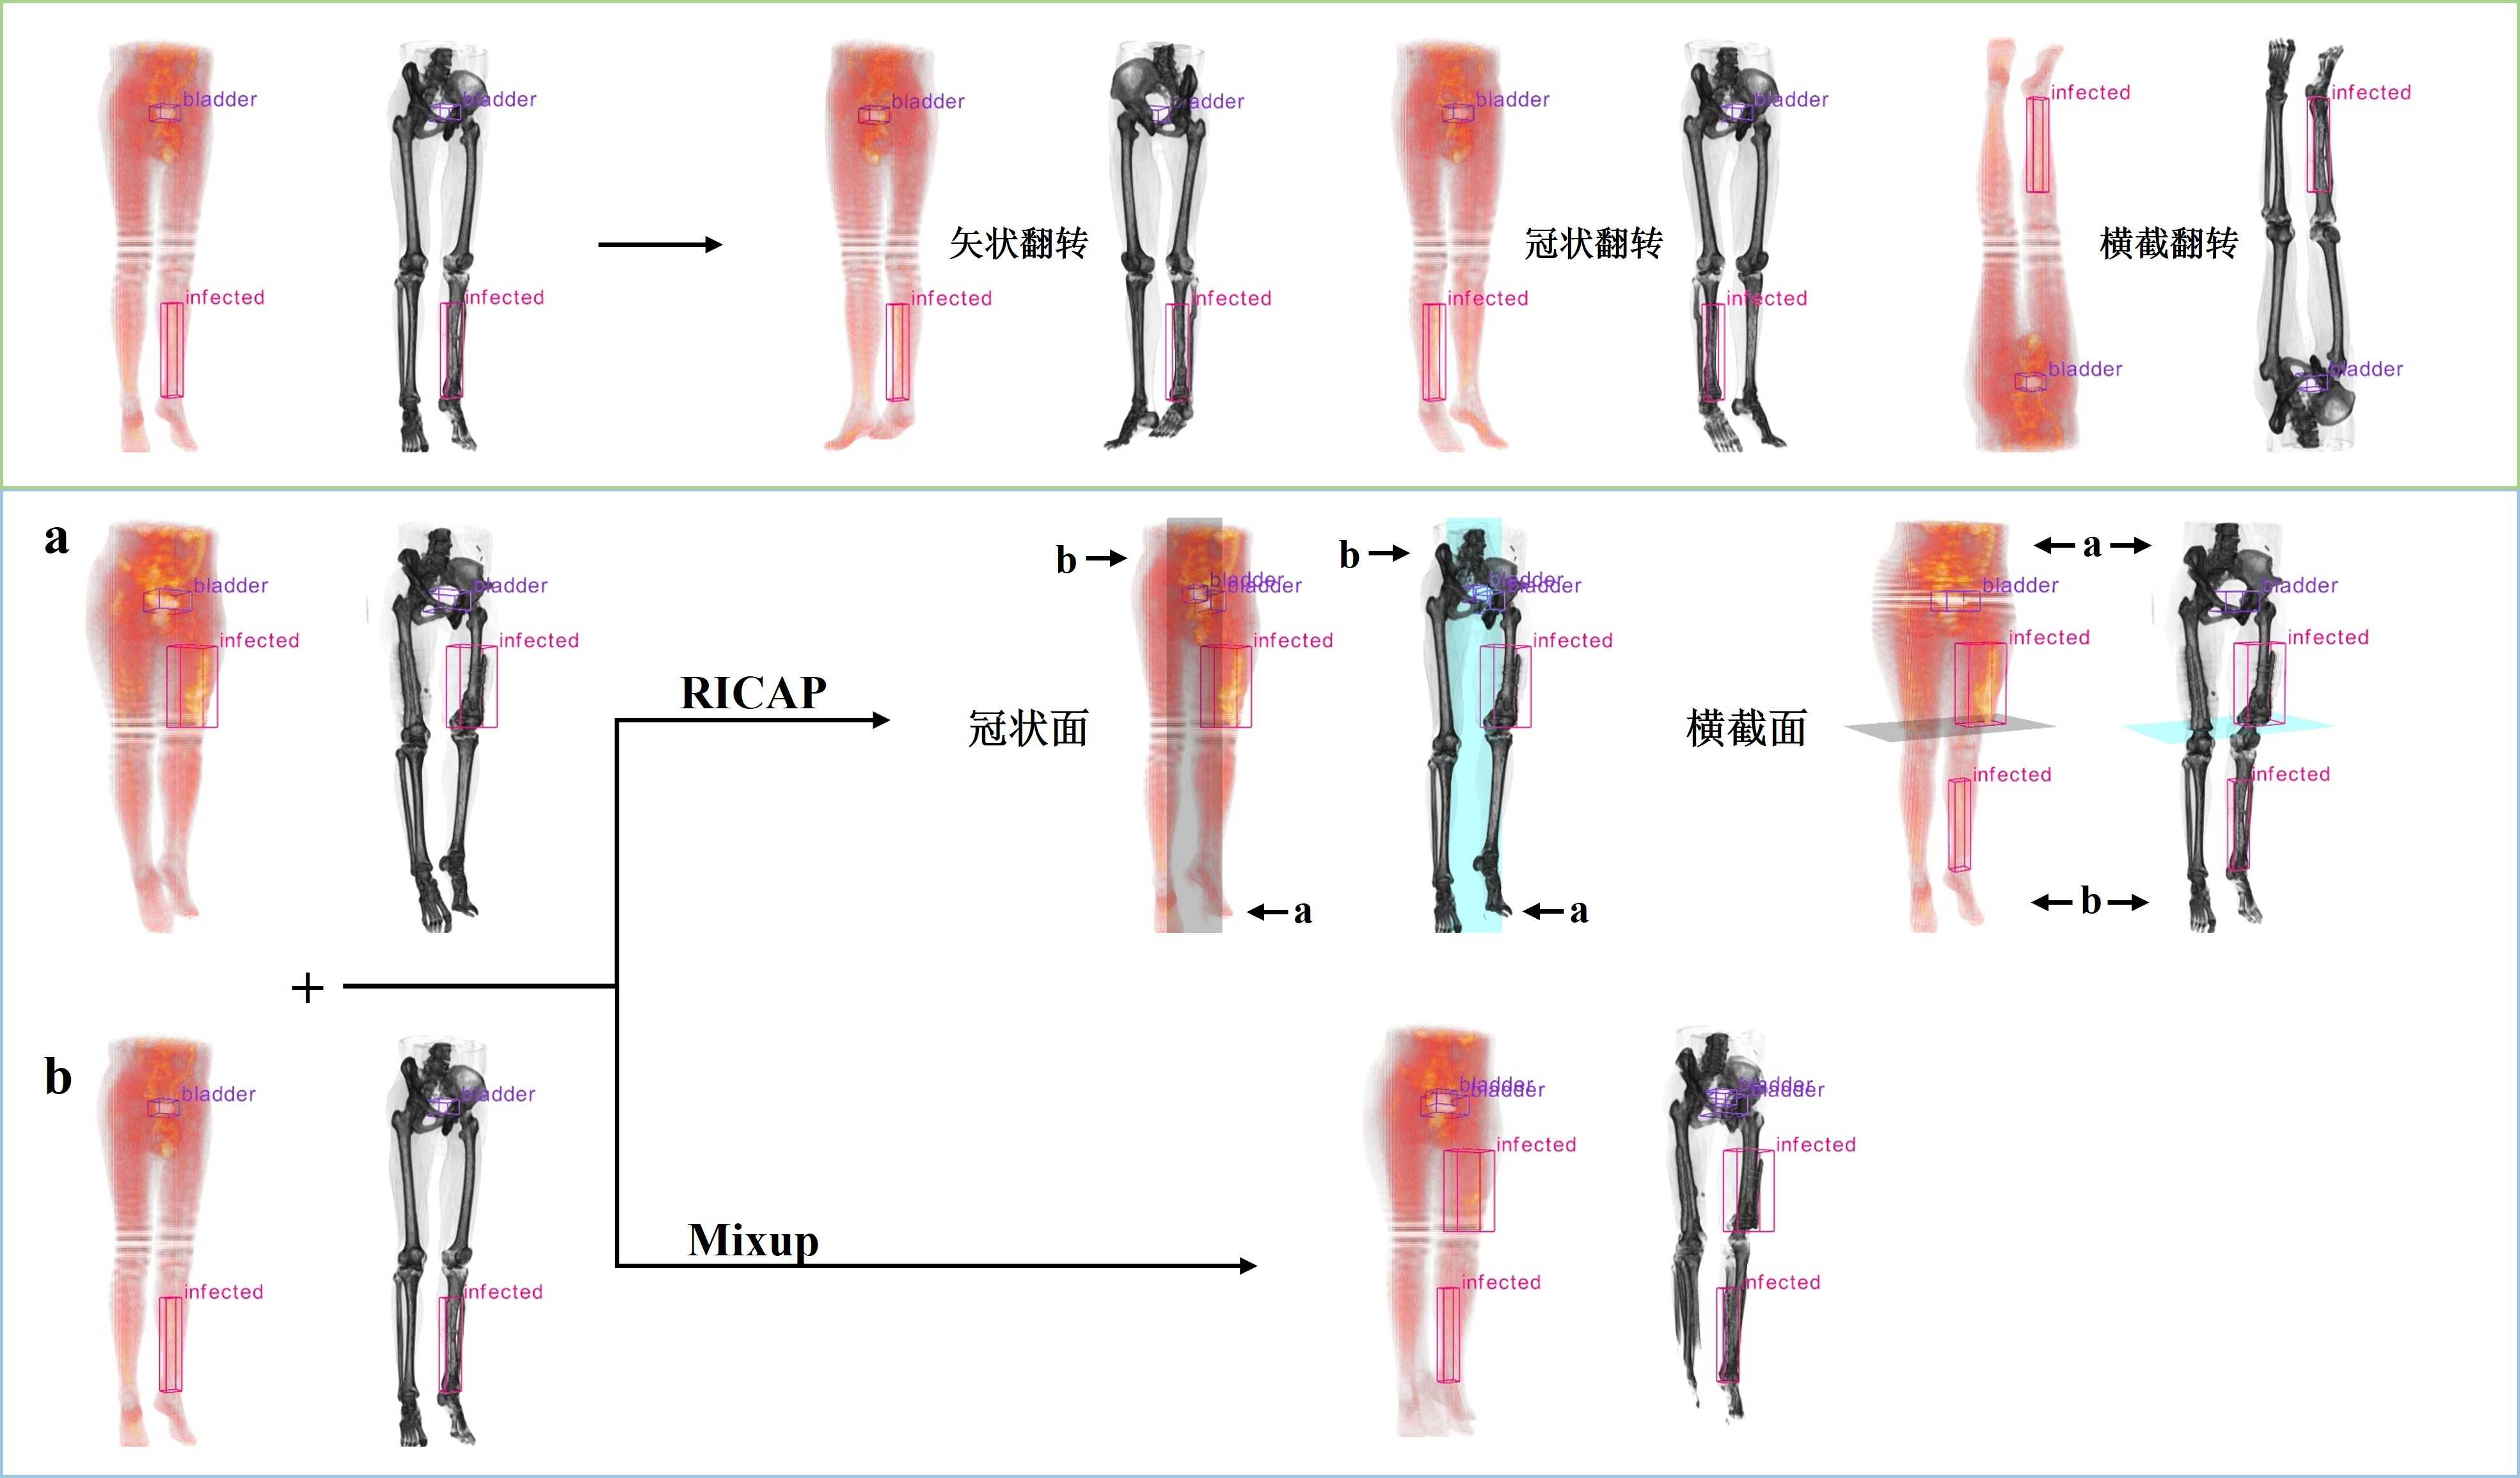
\includegraphics[height=\textwidth, width=0.95\textheight,angle=90,keepaspectratio]{figures/chap04_augmentation.jpg}
  \caption{应用于PET/CT影像上的数据增强方法}
  \label{fig:chap04_augmentation}
\end{figure}

翻转属于单样本的数据增强方法,对单个样本随机地在矢状轴、管状轴和横断轴中一个方向上翻转。而Mixup和RICAP则是属于多样本的数据增强方法,通过各自地方法使用两个样本去合成一个新的样本。

Mixup的基本原理是通过对多个输入样本及其标签进行相同比例的混合,从而生成新的输入样本和标签。由此,在本章研究中,为了将原用于分类任务中的Mixup应用于目标检测任务,Mixup数据增强方法进行了适应性地修改。对于两个输入样本\(image_1\)和\(image_2\)以及它们的标签\(box_1\)和\(box_2\),输入样本进行等比例的混合生成新的输入样本\(image_{new}\),而标签采用并集的方式合成新的标签\(box_{new}\),如公式\ref{eq:chap04_mixup}所示:
\begin{equation}
  \begin{aligned}
    image_{new} & = 0.5 \times image_1 + 0.5 \times image_2 \\
    box_{new}   & = box_1 \cup box_2
  \end{aligned}
  \label{eq:chap04_mixup}
\end{equation}

RICAP的基本原理是通过多个输入样本按照不同的所占区域下进行裁剪,裁剪得到的样本按照所占区域的相对位置进行拼接生成新的输入样本,而标签则按照它们输入样本所占区域占新样本总体区域的大小为比例进行混合生成新标签。由此,在本章研究中,同样适用于分类任务中的RICAP进行了适应性地修改,以更加适合于骨折相关感染病灶检测任务。首先,随机地在矢状轴和横断轴方向上二选一。随后,在选中的方向上随机地选择需要裁剪的区域。最后,根据裁剪区域的相对位置拼接裁剪下来的输入样本生成新的输入样本。裁剪区域的计算方式如下:

假设输入样本的大小为\((W,H,D)\)。如果在矢状轴上进行裁剪与拼接,则对于两个输入样本的裁剪区域分别为\((1, 1, 1)\thicksim (\omega, H, D)\)和\((\omega + 1, 1, 1)\thicksim (W, H, D)\)。如果在横断轴上进行裁剪,则对于两个输入样本的裁剪区域分别为\((1, 1, 1)\thicksim (W, H, \delta)\)和\((1, 1, \delta + 1)\thicksim (W, H, D)\)。其中,\(\omega\)和\(\delta\)的计算方式如\ref{eq:chap04_ricap}所示。
\begin{equation}
  \begin{aligned}
    \omega & = round(\omega) & \quad \omega & \sim U(0.4\times W, 0.6 \times W) \\
    \delta & = round(\delta) & \quad \delta & \sim U(0.4\times D, 0.6 \times D) \\
  \end{aligned}
  \label{eq:chap04_ricap}
\end{equation}
其中,\(round(\cdot)\)表示取整函数,\(X \sim U(a, b)\)表示\(X\)服从区间\((a,b)\)上的均匀分布。

\section{框架设计}

\begin{figure}
  \centering
  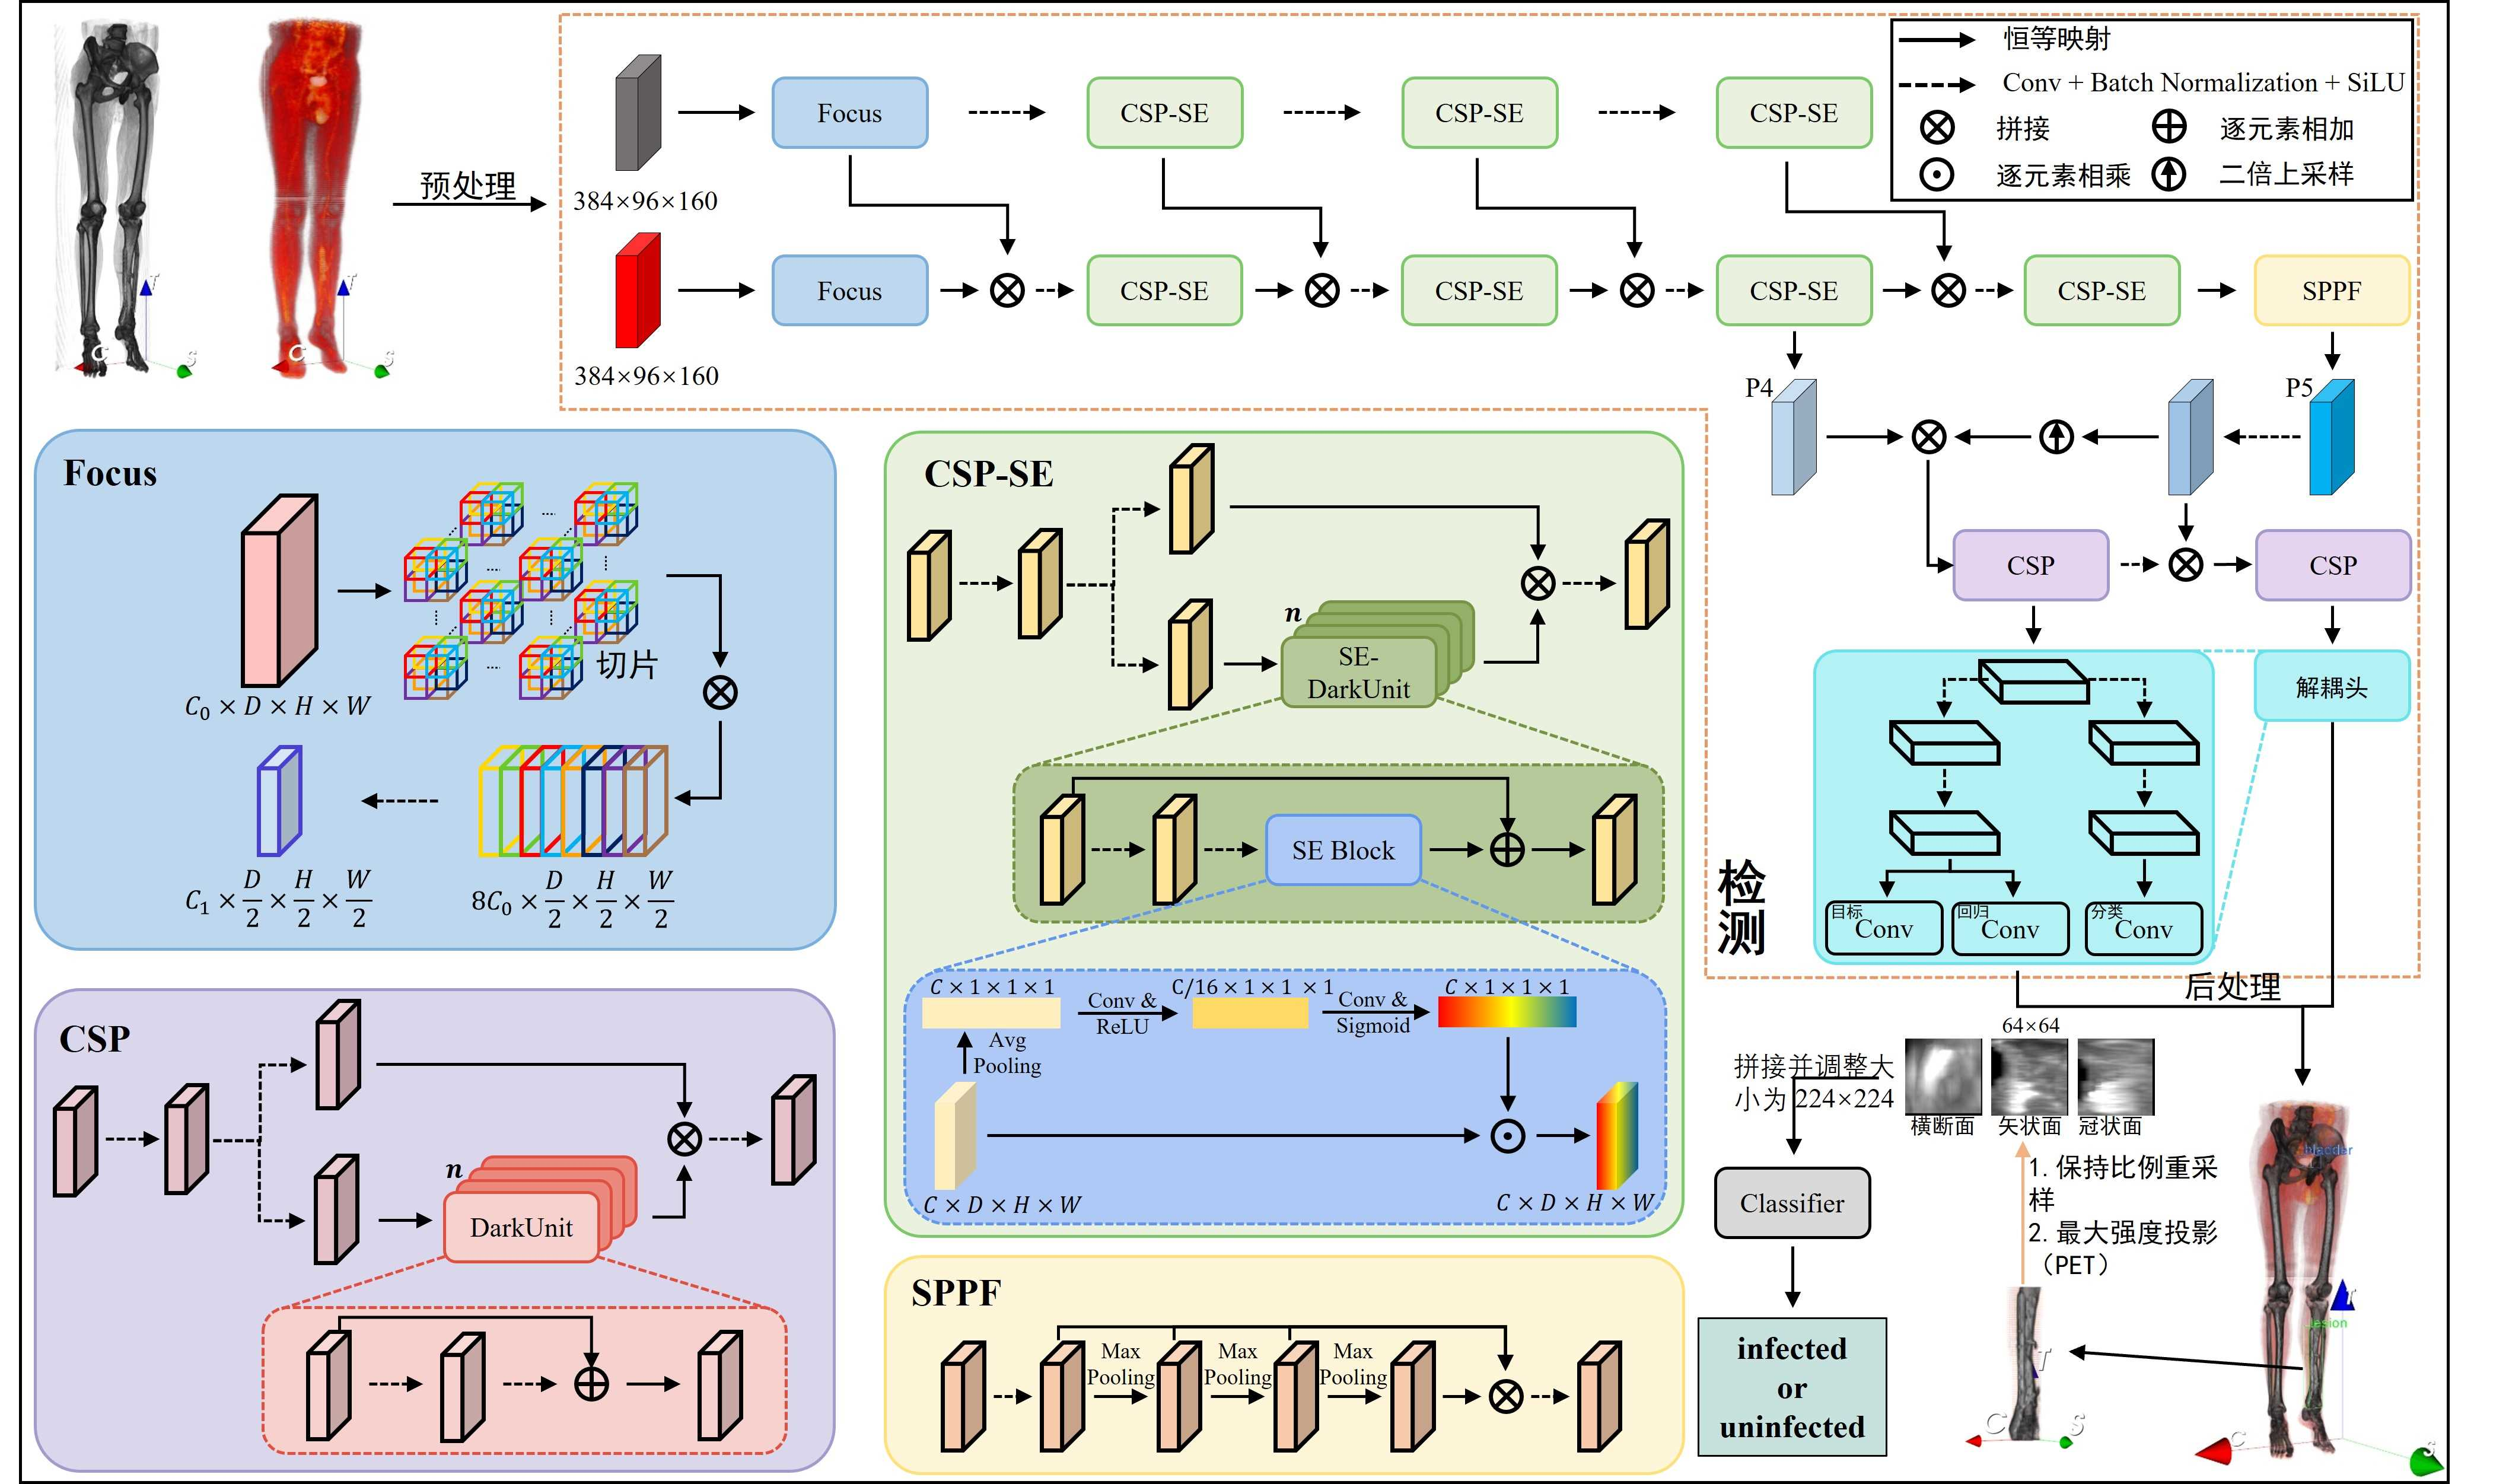
\includegraphics[width=0.95\textheight,height=\textwidth,angle=90,keepaspectratio]{figures/chap04_model.jpg}
  \caption{两阶段的病灶检测诊断分类网络框架示意图}
  \label{fig:chap04_model}
\end{figure}

PET/CT影像是两种模态组合的三维影像数据,它们展示了一个患者在注射药剂后的解剖组织信息和生理代谢信息。针对PET与CT影像之间存在互补互助的特性。本章在骨折相关感染的诊断方法中设计了一个两阶段的病灶检测诊断分类网络框架3DFRINet,整体架构如图\ref{fig:chap04_model}所示。整个网络框架分为病灶检测网络与病灶诊断分类网络,采用先检测后分类的两阶段网络框架的设计,可以排除掉与病灶无关的大部分区域,使得病灶诊断分类网络更加关注于病灶区域的生理代谢信息。病灶检测网络322-YOLO(3 dimensions 2 paths 2 heads YOLO)通过双分支设计和注意力模块,进一步优化对骨折相关感染病灶的定位。按照YOLO的结构设计也提高网络对于小尺度和多尺度病灶的检测精度,同时有效地减少了错检率。病灶诊断分类网络对候选区域进一步挖掘病灶的代谢形态特征,实现对骨折相关感染的准确分类。

\subsection{病灶检测网络322-YOLO}

经过本章引入的预处理流程后,将PET和CT影像数据重采样至\(384 \times 96\times 160\),并将CT的HU以300为窗位,1500为窗宽进行归一化,PET的SUV中小于0的统一为0。随后,被输入到322-YOLO病灶检测网络,对骨折相关感染病灶区域进行检测和识别。322-YOLO在YOLOX\cite{ge2021yolox}的基础上改进而来,由用于特征提取的双分支主干网络,整合两个不同层次下的特征图的颈部网络以及用于预测目标的种类、大小和位置的头部网络组成。

双分支主干网络可以分为PET主分支和CT辅助分支,当PET主分支持续提取生理代谢信息特征的同时,来自于CT辅助分支的解剖信息特征也被逐阶段地融入生理代谢信息特征之中。PET主分支主要由Focus、CSP-SE和SPPF模块构成,而CT辅助分支主要由Focus和CSP-SE模块构成。Focus模块从三个维度上以一个体素间隔对输入数据进行切片,随后拼接切片得到的8个子块,然后通过卷积进行特征提取与下采样。它将PET中的生理信息和CT中的解剖信息从空间维度堆叠到通道维度,在不牺牲特征信息的前提下,提高卷积操作对生理和解剖信息的感知范围,为网络提供了更广泛的上下文信息,有助于准确定位和识别感染病灶。CSP-SE模块(the Cross Stage Partial-Squeeze and Excitation dark unit)在dark unit的基础上结合了跨阶段部分结构\cite{wang2020cspnet}和通道注意力模块\cite{hu2018squeeze}。跨阶段部分结构允许特征在不同层之间进行更有效的信息传递和融合,有助于捕捉不同尺度和抽象级别的特征。同时,通道注意力模块的引入使得CSP-SE模块能够根据特定通道的重要性调整特征的权重,进一步提升网络对骨折相关感染病灶的关注度。通过充分结合了多层次的特征表达和通道级的信息调控,为网络在处理骨折相关感染特征上提供了更为丰富和精准的上下文信息。SPPF模块是由SPP\cite{he2015spatial}改进而来,具有更少的参数,更快的计算速度。它可以整合不同尺度的特征,以更好地适应骨折相关感染病灶的多样性(例如病灶区域大小、生理代谢或解剖结构上的差异),减轻对单一尺度特征的过度依赖,全面地捕捉病灶区域的上下文信息。

用于训练模型的输入样本为\(\text{SUV}, \text{HU} \in R^{C \times D \times H \times W}\),其中\(C,D,H,W\)分为是输入样本的通道数、深度、高度和宽度。由于正负样本存在极度不平衡的问题,因此病灶检测网络不再使用最大的同时也是正负样本最不平衡的特征图\(P_3\)。则由双分支主干网络提取的两个尺度下的特征图\(P_4\)和\(P_5\)的计算方式如\ref{eq:chap04_backbone}所示。
\begin{equation}
  \begin{aligned}
    P_1^{HU}  & = \text{Focus}(HU) \quad P_1^{SUV} = \text{Focus}(SUV)         \\
    P_i^{HU}  & = \text{CSP-SE}(\text{CBS}(P^{HU}_{i-1}))                      \\
    P_j^{SUV} & = \text{CSP-SE}(\text{CBS}(P^{HU}_{j-1} \oplus P^{SUV}_{j-1})) \\
    P_4       & = P_4^{SUV} \quad P_5 = \text{SPPF}(P_5^{SUV})
  \end{aligned}
  \label{eq:chap04_backbone}
\end{equation}
其中,\(P_i^{HU}(i=2,3,4)\)表示为第\(i\)阶段中CT辅助分支提取的特征图,\(P_j^{SUV}(j=2,3,4,5)\)表示为第\(j\)阶段中PET主分支融合并提取的特征图,CBS表示一个由卷积、批归一化和SiLU构成的基础模块,\(\oplus\)表示拼接操作。

颈部网络的结构由自顶向下和自底向上两条路径组成,以融合不同层次下的特征图,来提高对病灶的准确定位和识别。自顶向下的路径通过将丰富的语义信息(例如目标的类别信息)传播到浅层特征图,为网络提供更高层次的语义理解。与此同时,自底向上的路径则将目标的位置和大小信息传递到深层特征图,使得不同层次的特征在融合后既包含丰富的目标类别特征,又包含位置和大小信息。这种双向信息传递的机制有助于更全面地捕捉感染病变的特征,从而提高检测准确性。与此同时,自底向上的路径聚合了所有特征层的路径,从而缩短了底层与顶层特征之间的距离。这样的结构有助于更快地传播底层特征到上层,提高了网络对于病灶不同层次特征的有效利用,增强了整体网络的表达能力。通过自顶向下的路径计算得到\(P_4^{neck}\)和自底向上的路径计算得到\(P_5^{neck}\),如\ref{eq:chap04_neck}所示。
\begin{equation}
  \begin{aligned}
    P_4^{neck} & = \text{CSP}(\text{Upsample}(\text{CBS}(P_5)) \oplus P_4)    \\
    P_5^{neck} & =  \text{CSP}(\text{CBS}(P_5) \oplus \text{CBS}(P_4^{neck}))
  \end{aligned}
  \label{eq:chap04_neck}
\end{equation}
其中,Upsample表示2倍上采样。

头部网络采用解耦的模式,通过在颈部网络融合的特征中独立地进行目标的类别、位置和大小的预测,有效减少了不同预测任务之间的互相干扰。这种解耦设计使得模型可以更准确地预测定位目标的类别,同时在空间上准确定位病灶的位置和大小,从而提高了整体检测性能。其计算方式如\ref{eq:chap04_head}所示。
\begin{equation}
  \begin{aligned}
    P_c   & = \text{CBS}(\text{CBS}(P_n^{neck})) \\
    cls_n & = Conv_1(P_c)                        \\
    P_r   & = \text{CBS}(\text{CBS}(P_n^{neck})) \\
    reg_n & = Conv_2(P_r)                        \\
    obj_n & = Conv_3(P_r)                        \\
  \end{aligned}
  \label{eq:chap04_head}
\end{equation}



(1)无先验框

322-YOLO跟YOLOX一致,采用了无先验框的方式,但在YOLOX的基础上添加了需要预测的值。在解耦头中,独立预测的目标类别设置为2类,分别是病灶和膀胱;目标大小从4个值改成了6个值,即预测框在三维网格中位于左上后方的三个偏移量以及预测框的宽、高和深。在检测网络最终预测的不同层次下的特征图中,根据目标的中心位置以及预定义的范围去分配相应的正样本。

(2)分配策略

322-YOLO跟YOLOX在正样本分配策略上的一致,作为一个无先验框的目标检测方法,对每一个目标不仅仅只分配一个位于中心位置的正样本,同时还关注其他高质量的预测。通过关注这些高质量的预测也可能带来有益的梯度,这从一定程度上来说可以缓解训练过程中正负样本的极端不平衡。简单地来说,322-YOLO通过将以目标的中心位置为中心点,以2.5为半径的正方体区域设置为正样本,同时也将目标框中的区域设置为正样本。这中正样本分配方式一定程度上可以提升目标检测器的检测性能。

在目标检测任务中,标签分配策略也是很重要的一部分。SimOTA是OTA(Optimal Transport Assignment)\cite{ge2021ota}的一种简化近似版本。OTA是从一个全局视角中去分析标签分配的方式并将分配过程表述为最优传输问题(Optimal Transport)。通过免去手工选定参数的方式,使得真实框匹配多个更加合适的多个预测框。SimOTA将OTA的优化过程简化为动态top-k策略。首先,计算每个真实框与预测框之间的成对匹配度\(c\),通过使用预测框\(p_n\)与真实框\(g_m\)损失来表示,如公式:
\begin{equation}
  c_{mn} = L^{cls}_{mn} + \lambda L^{reg}_{mn}
\end{equation}
其中,\(\lambda\)表示平衡系数,\(L^{cls}_{mn}\)和\(L^{reg}_{mn}\)是真实框\(g_m\)与预测框\(p_n\)之间的分类损失和回归损失。对于每个真实框,进一步地在满足前面所述的正样本分配策略的基础上,选择具有前k个最小的成对匹配度的预测框。其中,成对匹配度越低表示真实框与预测框越合适。最终,将这些满足条件的预测框所在特征图的网格位置设置为正样本,其他的网格设置为负样本。

(3)损失函数

通过SimOTA标签分配策略对每个目标都分配相应的正负样本之后,二元交叉熵损失函数(Binary Cross Entropy Loss)用于计算区分正负样本的损失\(\mathcal{L}_{obj}\)和目标类别的损失\(\mathcal{L}_{cls}\),交并比损失函数(IoU Loss)用于计算目标尺寸大小的损失\(\mathcal{L}_{reg}\)。对于预测框\(p = (p^{obj}, p^{cls}, p^{reg})\)和真实框\(g = (g^{obj}, g^{cls}, g^{reg})\),三种损失的计算方式如\ref{eq:chap04_loss1}所示。
\begin{equation}
  \begin{aligned}
    \mathcal{L}_{obj} & = -\sum_{i=0}^I( g^{obj}_{bi} \log p^{obj}_{bi} +  (1- g^{obj}_{bi})\log(1-p^{obj}_{bi} ))      \\
    \mathcal{L}_{cls} & = -\sum_{k=0}^K( g^{cls}_{bk} \log p^{cls}_{bk} +  (1- g^{cls}_{bk})\log(1-p^{cls}_{bk} ))      \\
    \mathcal{L}_{reg} & = \sum_{k=0}^K( 1 - (\frac{g^{reg}_{bk} \cap p^{reg}_{bk}}{g^{reg}_{bk} \cup p^{reg}_{bk}})^2 ) \\
  \end{aligned}
  \label{eq:chap04_loss1}
\end{equation}
其中,\(I\)表示所有预测框的数量,\(K\)表示SimOTA标签分配策略对每个真实框匹配到的相应的正样本的数量。最终的损失函数计算如下:
\begin{equation}
  \mathcal{L}  = \mathcal{L}_{obj} + \mathcal{L}_{cls} + 5 \times \mathcal{L}_{reg}
\end{equation}

\subsection{病灶诊断分类网络}

\begin{figure}[b]
  \centering
  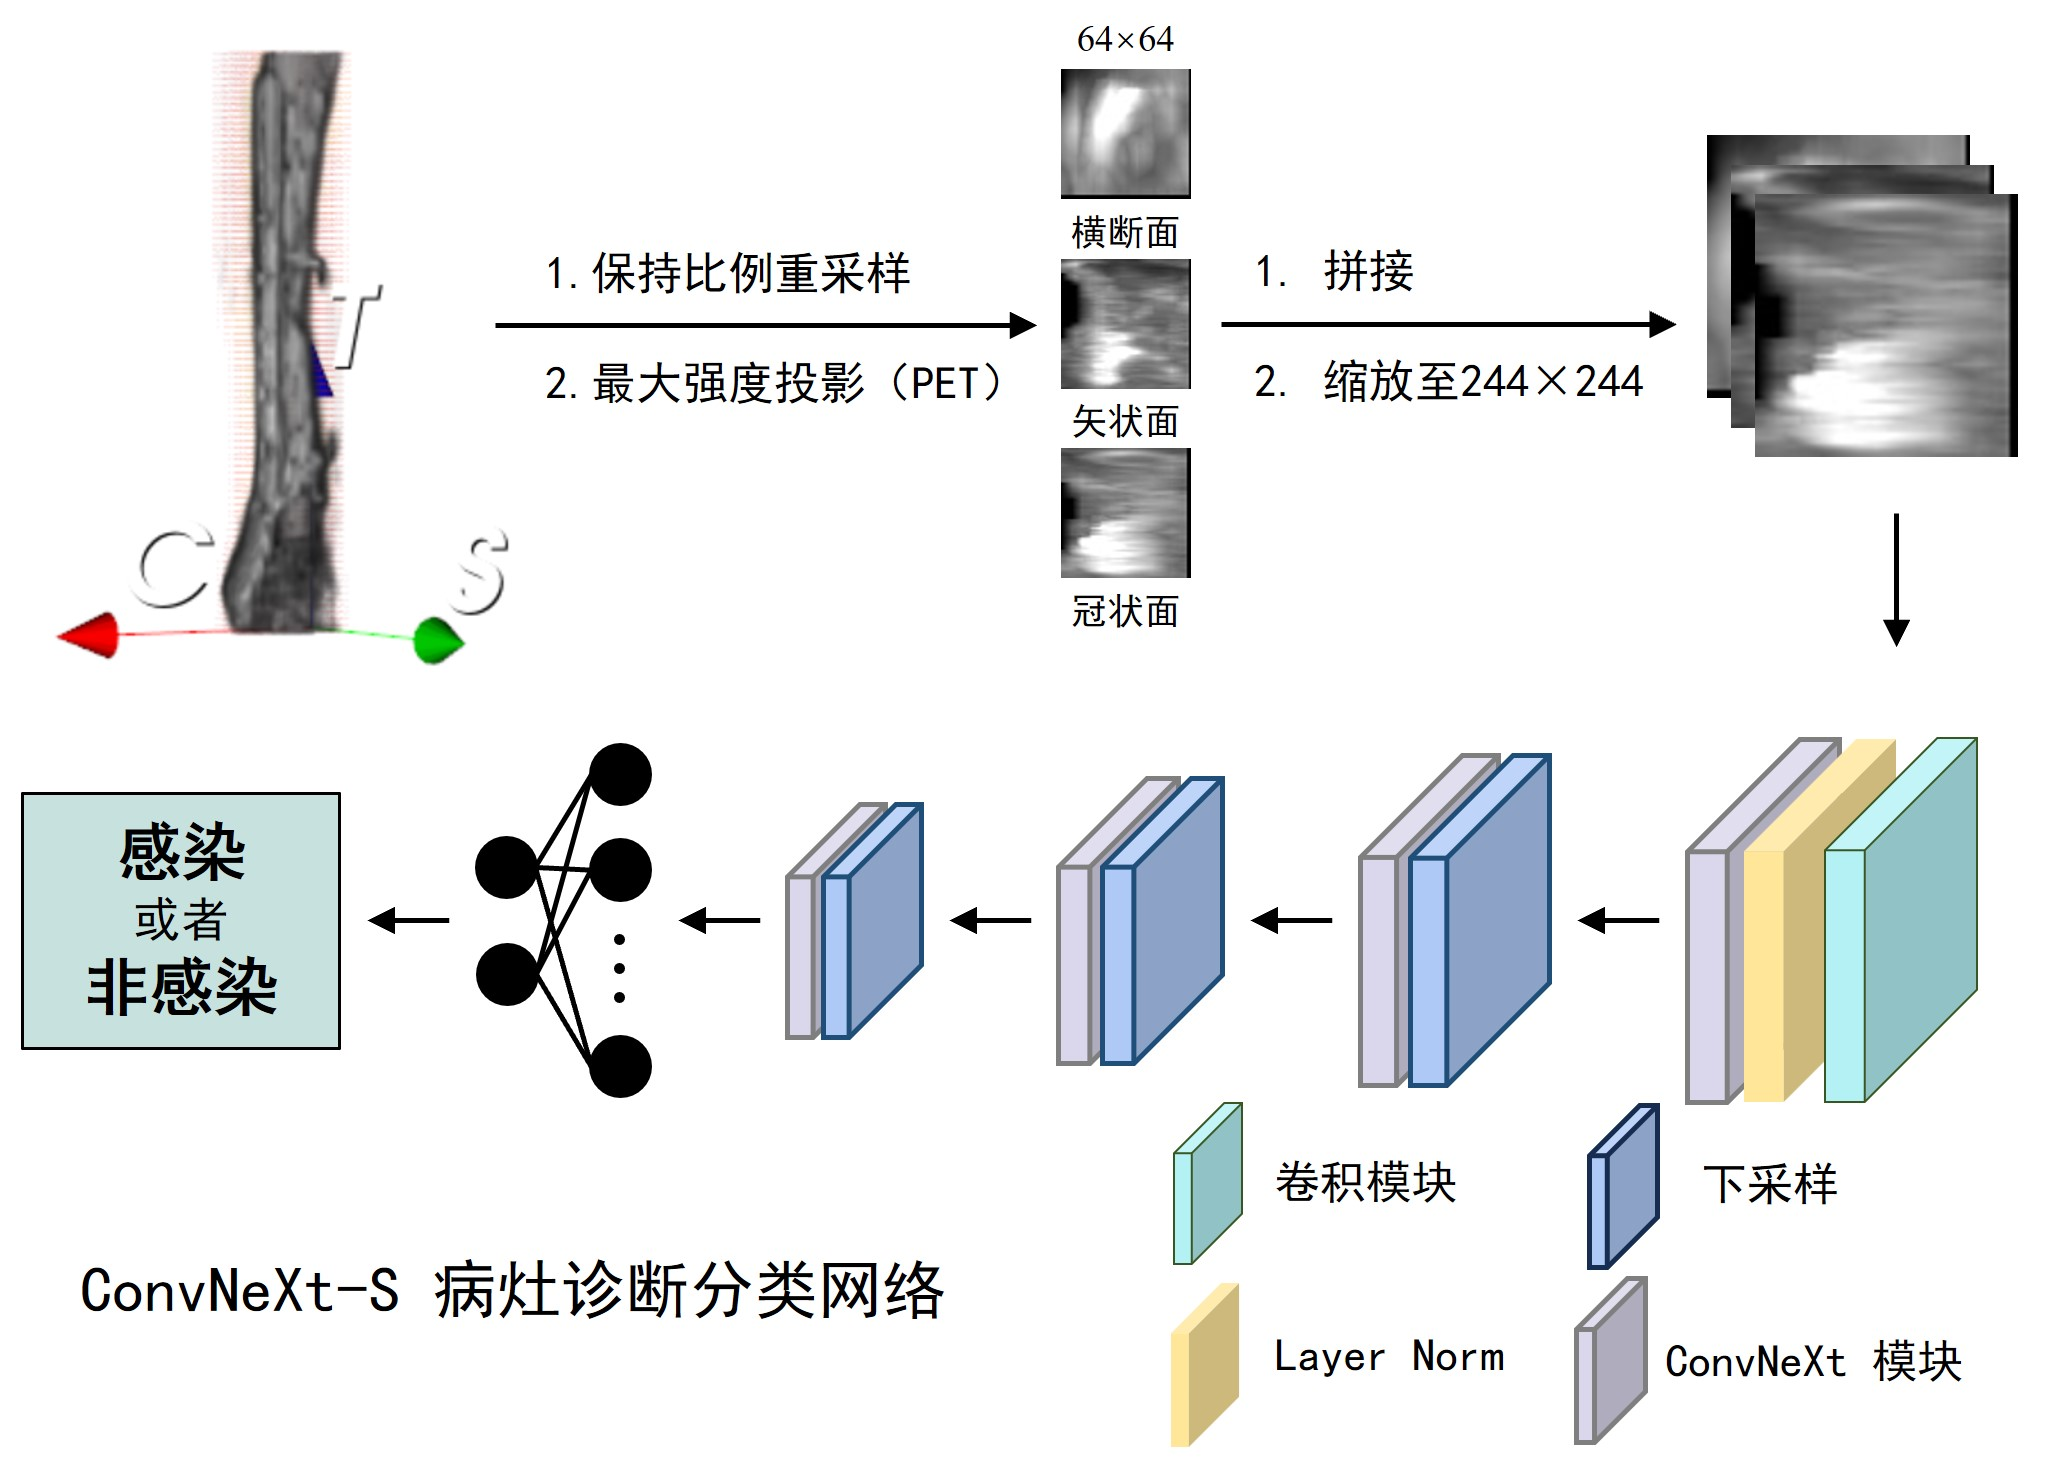
\includegraphics[width=0.6\textwidth]{figures/chap04_classifier.jpg}
  \caption{病灶诊断分类网络}
  \label{fig:chap04_classifier}
\end{figure}

首先,设置置信度阈值为0.1,最大输出的检测框数量为100,让目标检测网络322-YOLO输出所有符合条件的预测框。然后,设置交并比阈值为0.01,去除掉相同类别下重叠程度高于交并比阈值的预测框。最后,筛选得到类别为病灶的预测框。

根据得到的病灶预测框,在预处理后的PET影像上进行裁剪,得到病灶区域的PET影像。然后对病灶区域的PET影像进行等比例的缩放并在四周进行填充,使得最终获得的PET影像为\(64\times64\times64\)的大小,并将PET的SUV中小于0的设置为0。其中,PET中填充区域的值为0。在矢状轴、冠状轴和横断轴上进行最大强度投影得到的三张单通道图像拼接成一张三通道图像,并重采样至\(244 \times 244\)的大小后,输入到病灶诊断分类网络ConvNeXt-S之中,对病灶区域进行诊断分类,如图\ref{fig:chap04_classifier}所示。

将训练模型的图像输入到ConvNeXt-S诊断分类网络中,经过ConvNeXt-S的卷积层、Layer norm层、ConvNeXt模块、下采样层、平均池化层和全连接层得到最终的诊断分类结果。其中,在训练过程中,使用了镜像(水平或翻转)和Mixup来弥补数据集不足的问题,损失函数采用的是焦点损失函数(Focal Loss)。

\section{实验}

\subsection{实验环境}

本章所有实验均使用PAI上海大学机器学习平台上进行。学习平台配置:两个NVIDIA Tesla V100(32GB) GPU;Linux Ubuntu 20.04.2 操作系统;Pytorch 1.8.0 深度学习框架;Python 3.8.17 编程语言。具体详细的配置信息与上一章节一致。

\subsection{数据集}

\begin{table}[htbp]
  \centering
  \caption{下肢骨折相关感染的PET/CT影像数据集特征}
  \begin{tabular}{lc}
    \toprule
    特征         & 数量       \\
    \midrule
    骨折类别,数量(\%)      \\
    \quad 股骨   & 91 (30.5)  \\
    \quad 胫腓骨 & 169 (56.7) \\
    \quad 足     & 36 (12.1)  \\
    \quad 下肢   & 2 (0.7)    \\
    诊断结果,数量(\%)      \\
    \quad 感染   & 190 (63.8) \\
    \quad 非感染 & 108 (36.2) \\
    \bottomrule
  \end{tabular}
  \label{tab:chap04_dataset}
\end{table}

本章采用的下肢骨折相关感染的PET/CT影像数据集由本文作者与上海市第六人民医院核医学科合作构建。纳入数据集的标准:存在既往的下肢骨折手术治疗;存在术后症状,如疼痛、活动受限或红肿;进行过\(^{18}\)F-FDG PET/CT扫描;\(^{18}\)F-FDG PET/CT扫描时间与既往手术之间的时间间隔超过3个月;\(^{18}\)F-FDG PET/CT扫描时间与手术后的时间间隔少于1个月。排除标准:存在鼻窦道、脓等典型感染的临床表现;术后未行常规细菌培养以及病理分析;\(^{18}\)F-FDG PET/CT扫描前一周内使用抗生素;不完整的临床数据;现有资料不能确定最终诊断。在数据集方面,一共纳入了从2016年11月到2021年12月之间303名潜在合格的患者。在阅览所有患者的PET/CT影像后,22名患者因为影像缺失或不完整被排除掉。最终,具有298个病灶区域的281名患者被纳入本章的研究中,详细信息如表\ref{tab:chap04_dataset}所示。本章研究中所有患者骨折相关感染的最终诊断是基于手术中深部组织提取后的医学微生物培养或组织病理学分析以及至少6个月的临床随访。

\subsection{评价指标}

假体关节感染任务包含目标检测和分类问题。在目标检测任务中,本章选用了平均精度(Average Precision,AP)、精确率(Precision)、召回率(Recall)和F1值(F1 score),如式\ref{eq:chap04_metric}所示。
\begin{equation}
  \begin{aligned}
    Precision & = \frac{TP}{TP+FP}                                                   \\
    Recall    & = \frac{TP}{TP+FN}                                                   \\
    F1 socre  & = \frac{2 \times Precision \times Recall}{Precision + Recall}        \\
    AP        & = \sum_{r_i}(Recall_{r_i} - Recall_{r_{i-1}}) \times Precision_{r_i} \\
  \end{aligned}
  \label{eq:chap04_metric}
\end{equation}
其中,\(TP\)(True Positive)是被正确检测为正类别的样本数量,\(FP\)(False Positive)是被错误检测为正类别的样本数量,\(FN\)(False Negative)是被错误地标记为负类别的样本数量。\(Recall_{r_i}, Precision_{r_i}\)表示根据模型输出和真实标签,在置信度为\(r_i\)下的精确率和召回率。平均精度衡量了在不同置信度阈值下目标检测网络的精确率和召回率之间的平衡,是一个综合性指标;精确率表示预测为正类别的样本中实际为正类别的比例;召回率表示实际为正类别的样本中被正确预测为正类别的比例。分类任务采用的评估指标有Acc,Spec,Sen,PPV,NPV,F1,AUC与上一个章节一致。Acc评估下肢假体关节感染的诊断准确率;Spec评估实际不患骨折相关感染的患者诊断未未感染的概率;Sen评估实际患有骨折相关感染的患者诊断为感染的概率。PPV评估被诊断为骨折相关感染的患者实际患有的概率;NPV评估被诊断未患骨折相关感染的患者实际未感染的概率。F1是PPV和Sen的综合评价指标,AUC是敏感性和特异性在不同阈值设定下生成的ROC曲线下的面积。

\subsection{实验结果}

\begin{table}[htbp]
  \centering
  \caption{病灶检测网络与YOLO系列模型在病灶上的检测性能比较}
  \resizebox{\textwidth}{!}{
    \begin{tabular}{lccccccccccc}
      \toprule
      模型     & AP\(_{25:75}\)  & AP\(_{25}\)     & Precision\(_{25}\) & Recall\(_{25}\) & F1\(_{25}\)     & AP\(_{50}\)     & Precision\(_{50}\) & Recall\(_{50}\) & F1\(_{50}\)     & flops   & params  \\
      \midrule
      YOLOv3   & 0.1941          & 0.5656          & 0.6842             & 0.6290          & 0.6566          & 0.1152          & 0.1579             & 0.1452          & 0.1515          & 368.79G & 172.95M \\
      YOLOv4   & 0.2553          & 0.7377          & 0.8000             & 0.7742          & 0.7871          & 0.1405          & 0.2667             & 0.2581          & 0.2624          & 278.54G & 170.69M \\
      YOLOv5-S & 0.2019          & 0.6876          & 0.7377             & 0.7258          & 0.7318          & 0.0540          & 0.1803             & 0.1774          & 0.1789          & 35.65G  & 15.84M  \\
      YOLOv5-M & 0.2475          & 0.7265          & 0.7460             & 0.7581          & 0.7520          & 0.1644          & 0.3016             & 0.3065          & 0.3040          & 99.17G  & 50.12M  \\
      YOLOv5-L & 0.2113          & 0.7109          & 0.6957             & 0.7742          & 0.7349          & 0.0963          & 0.1884             & 0.2097          & 0.1990          & 216.93G & 114.87M \\
      YOLOX-S  & 0.3286          & 0.8085          & 0.8154             & 0.8548          & 0.8351          & 0.3032          & \textbf{0.4154}    & 0.4355          & \textbf{0.4254} & 59.15G  & 21.24M  \\
      YOLOX-M  & 0.3673          & 0.8049          & \textbf{0.8281}    & 0.8548          & 0.8415          & \textbf{0.3073} & 0.4063             & 0.4194          & 0.4128          & 152.03G & 62.29M  \\
      YOLOX-L  & 0.3069          & 0.7892          & 0.8000             & 0.8387          & 0.8194          & 0.1738          & 0.3077             & 0.3226          & 0.3151          & 310.91G & 136.53M \\
      322-YOLO & \textbf{0.3834} & \textbf{0.9234} & 0.8000             & \textbf{0.9677} & \textbf{0.8839} & 0.3041          & 0.3600             & \textbf{0.4355} & 0.3977          & 63.71G  & 26.04M  \\
      \bottomrule
      \multicolumn{12}{l}{\footnotesize *\(_{25:75}\)表示在IoU\(\in [0.25,0.75]\)以0.05为步长时*的平均值;*\(_{25}\)表示在IoU=0.25时*;*\(_{50}\)表示在IoU=0.50时*;}
    \end{tabular}
  }
  \label{tab:chao04_experiment_yolo}
\end{table}

本章提出的病灶检测网络322-YOLO跟其他YOLO系列模型的病灶检测性能进行了比较,如表\ref{tab:chao04_experiment_yolo}所示。其中,为了YOLO系列模型适用于三维的PET/CT影像数据,将YOLO系列模型的预处理、模型结构、后处理部分中都从相应的二维操作修改为了三维操作。在综合检测性能上,322-YOLO不仅拥有较小的计算量和参数量,还表现出了最佳的病灶定位检测性能。此外,322-YOLO的计算量和参数量还不到在AP\(_{25:75}\)上排名第二的YOLOX-M的一半。在其他关于病灶检测性能的细分评估指标AP\(_{25}\)、Recall\(_{25}\)、F1\(_{25}\)和Recall\(_{50}\)中,322-YOLO都是最佳的。这表明322-YOLO在病灶检测、计算量和参数量上的综合表现能力最佳。值得说明的是,322-YOLO在验证集中检测到了75个病灶区域,其中有63个与专业医生标记的病灶区域相匹配,有9个是未标记的骨折相干感染病灶区域,只有3个是完全误检。

\begin{table}[htbp]
  \centering
  \caption{病灶检测网络322-YOLO的消融实验}
  \resizebox{\textwidth}{!}{
    \begin{tabular}{lcccccccc}
      \toprule
                          & \multicolumn{3}{c}{病灶} & \multicolumn{3}{c}{膀胱} & \multirow{2}{*}{flops} & \multirow{2}{*}{params}                                                       \\
                          & AP\(_{25:75}\)           & AP\(_{25}\)              & AP\(_{50}\)            & AP\(_{25:75}\)          & AP\(_{25}\)     & AP\(_{50}\)     &        &        \\
      \hline\hline
      YOLOX-S             & 0.3286                   & 0.8085                   & 0.3032                 & 0.7676                  & 1.0000          & 0.8418          & 59.15G & 21.24M \\
      \midrule
      + SPP→SPPF*         & 0.3390                   & 0.7829                   & 0.2812                 & 0.7543                  & 1.0000          & 0.8870          & 59.15G & 21.24M \\
      + only use P4/P5    & 0.3248                   & 0.8506                   & 0.1650                 & 0.7714                  & 1.0000          & 0.8487          & 35.08G & 18.22M \\
      + SE block          & 0.3610                   & 0.8943                   & 0.1965                 & 0.7523                  & 1.0000          & 0.8355          & 35.09G & 18.24M \\
      + two path backbone & 0.3895                   & 0.9105                   & 0.2746                 & 0.7442                  & 0.9643          & 0.8857          & 63.71G & 26.04M \\
      + Mixup             & \textbf{0.4084}          & 0.9010                   & 0.2795                 & 0.7341                  & 1.0000          & 0.8615          & 63.71G & 26.04M \\
      + RICAP             & 0.3834                   & \textbf{0.9234}          & \textbf{0.3041}        & 0.7456                  & \textbf{1.0000} & \textbf{0.9279} & 63.71G & 26.04M \\
      \bottomrule
    \end{tabular}
  }
  \label{tab:chao04_experiment_ablation}
\end{table}

为了验证病灶检测网络中多个改进方法的有效性,如模型结构、数据增强,本章设计了消融实验。实验步骤如下:1.采用YOLOX-S作为基准模型对下肢骨折相关感染PET/CT影像数据集进行训练验证;2.在1的基础上,将主干网络中最后一个阶段的特征提取模块由SPP+CSP的组合修改为CSP+SPPF的组合,即+ SPP→SPPF*;3.在2的基础上,仅采用主干网络中提取的P4和P5特征图,颈部网络和头部网络结构也进行相应的修改,即+ only use P4/P5;4.在3的基础上,在主干网络部分添加通道注意力模型模块(Squeeze and Excitation Block),即+ SE block;5.在4的基础上,将主干网络从单分支修改为双分支的结构设计,即+ two path backbone;6.在5的基础上,训练过程中动态地随机使用适应性修改的Mixup数据增强方法,即+ Mixup;7.在6的基础上,训练过程中再动态地随机使用适应性修改的RICAP数据增强方法,即+ RICAP。在表\ref{tab:chao04_experiment_ablation}中可以看出,在综合检测性能指标AP\(_{25:75}\)中,除了+ only use P4/P5以外,所有在模型结构上的改进方法对病灶检测网络的病灶检测性能都有所提升。对于+ only use P4/P5而言,计算量和参数量的减少,使得病灶检测性能上的下降是可以接受的。数据增强方法Mixup在AP\(_{25:75}\)上进一步提升了模型检测病灶的能力,而RICAP在AP\(_{25}\)和AP\(_{50}\)上进一步达到了最优的结果。通过病灶检测网络的消融实验可以得出,病灶检测性能AP\(_{25:75}\)提升了16.7\%,AP\(_{25}\)达到了0.9234,AP\(_{50}\)达到了0.3041,这表明了本章研究中针对病灶检测任务提出的所有改进方法的有效性。

\begin{table}[htbp]
  \centering
  \caption{带额外分类器的病灶检测网络与单一病灶检测网络的性能比较}
  \begin{tabular}{ccccccc}
    \toprule
                          & \multicolumn{3}{c}{感染} & \multicolumn{3}{c}{非感染}                                                               \\
                          & AP\(_{25}\)              & AP\(_{50}\)                & AP\(_{25:75}\) & AP\(_{25}\) & AP\(_{50}\) & AP\(_{25:75}\) \\
    \midrule
    322-YOLO              & 0.6395                   & 0.3108                     & 0.3129         & 0.2193      & 0.0022      & 0.0433         \\
    322-YOLO + Classifier & 0.8016                   & 0.3346                     & 0.3790         & 0.6330      & 0.1253      & 0.1808         \\
    \bottomrule
  \end{tabular}
  \label{tab:chao04_experiment_1vs2}
\end{table}

为了验证单阶段算法与双阶段算法的效果差异,进行了对比实验,如表\ref{tab:chao04_experiment_1vs2}所示。如果仅使用322-YOLO自身的类别预测来进一步细分病灶类别,病灶的检测效果较差。而采用两阶段的病灶检测诊断分类网络框架3DFRINet(322-YOLO + Classifier),即通过添加二阶段的病灶诊断分类网络对已定位的病灶进行进一步地细分,可以大大的提高病灶检测性能。与单阶段的322-YOLO的病灶检测性能相比,3DFRINet在感染病灶中的AP\(_{25}\)、AP\(_{50}\)和AP\(_{25:75}\)分别提升了25.35\%、7.66\%和21.12\%,在非感染病灶中的AP\(_{25}\)、AP\(_{50}\)和AP\(_{25:75}\)分别提升了188.65\%、5595.45\%和317.55\%。这进一步证明了添加一个额外的仅关注于病灶区域的分类器效果更好。

\begin{table}[htbp]
  \centering
  \caption{两阶段检测诊断框架3DFRINet与6名核医学医生的比较}
  \resizebox{\textwidth}{!}{
    \begin{tabular}{ccccccccc}
      \toprule
                                & Acc                & Spec               & Sen                & NPV                & PPV     & F1     & AUC    & \textit{p}      \\
      \hline\hline
      \multirow{2}{*}{3DFRINet} & 91.55\%            & 90.32\%            & 92.50\%            & 90.32\%            & 92.50\% & 0.9250 & 0.9331
                                & \multirow{2}{*}{-}                                                                                                              \\
                                & (83.10\%,97.18\%)  & (77.78\%,100.00\%) & (83.72\%,100.00\%) & (78.57\%,100.00\%) &
      (82.93\%,100.00\%)        & (0.8533,0.9756)    & (0.8547,0.9870)                                                                                            \\
      \midrule
      Junior 1                  & 74.65\%            & 93.55\%            & 60.00\%            & 64.44\%            & 92.31\% & 0.7273 & -      & \textbf{0.0018} \\
      Junior 2                  & 80.28\%            & 80.65\%            & 80.00\%            & 75.76\%            & 84.21\% & 0.8205 & -      & 0.0768          \\
      Junior 3                  & 74.65\%            & 77.42\%            & 72.50\%            & 68.57\%            & 80.56\% & 0.7632 & -      & \textbf{0.0075} \\
      Senior 1                  & 87.32\%            & 90.32\%            & 85.00\%            & 82.35\%            & 91.89\% & 0.8831 & -      & 0.4531          \\
      Senior 2                  & 85.92\%            & 90.32\%            & 82.50\%            & 80.00\%            & 91.67\% & 0.8684 & -      & 0.2188          \\
      Senior 3                  & 87.32\%            & 93.55\%            & 82.50\%            & 80.56\%            & 94.29\% & 0.8800 & -      & 0.3750          \\
      \bottomrule
    \end{tabular}
  }
  \label{tab:chao04_experiment_physician}
\end{table}

为了进行更加全面的对比评估实验,本章将提出的两阶段的病灶检测诊断分类网络框架3DFRINet与6名核医学影像科的临床医生进行比较。其中,有3名初级核医学医师和3名高级核医学医师。表\ref{tab:chao04_experiment_physician}展示了提出的3DFRINet的分类性能评估指标及其95\%的置信区间和6名核医学医师的诊断性能表现。从对比结果可以得出,3DFRINet拥有91.55\%的准确率、92.50\%的敏感率、90.32\%的阴性预测值和0.9250的F1上,均优于3名初级核医学医师和3名高级核医学医师。此外,其90.32\%特异率和92.50\%的阳性预测值都位列前三。这表明了3DFRINet相比较于3名初级核医学医师和3名高级核医学医师具有优秀的骨折相关感染诊断分类的性能表现。通过统计学分析,3DFRINet与两名初级核医学医生在准确率上的p值小于0.05,这说明3DFRINet与两名初级核医学医生在准确率上存在显著差异,而与1名初级核医学医师和3名高级核医学医师在准确率无显著差异。由此可知,3DFRINet具有与初级核医学医生更好或相同的诊断能力,与高级核医学医生相当的诊断性能。

\begin{figure}[htbp]
  \centering
  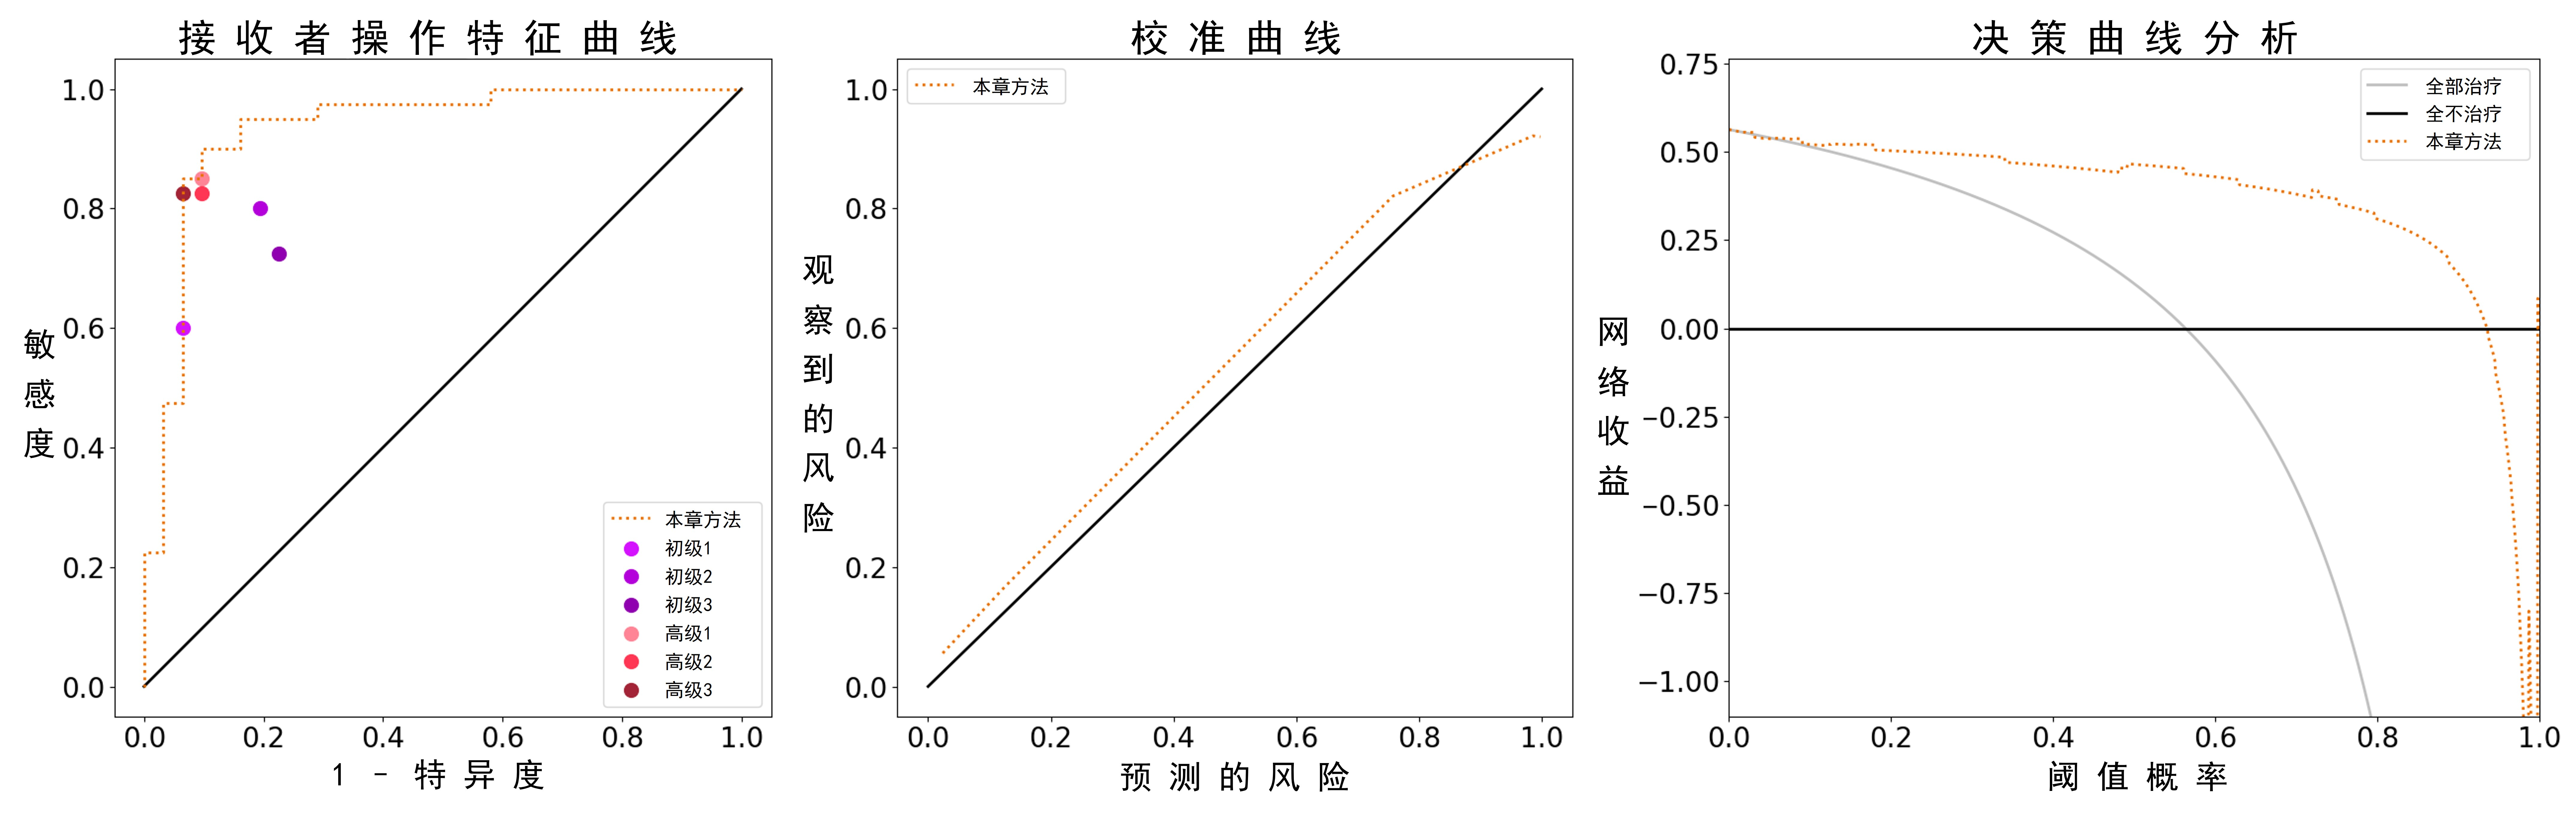
\includegraphics[width=\textwidth]{figures/chap04_eval.jpg}
  \caption{6名核医学医生与3DFRINet的ROC曲线;3DFRINet的标准曲线和决策曲线分析;}
  \label{fig:chap04_eval}
\end{figure}

如图\ref{fig:chap04_eval}所示,从ROC曲线上可以得出3DFRINet的诊断分类性能与三名高级核医学医师相当。3DFRINet的校准曲线较接近与45度对角线,这反映了在三维PET/CT影像上骨折相关感染的预测概率与骨折相关感染的真是改了具有良好的一致性。3DFRINet的决策曲线分析显示,网络在阈值概率较高的情况下存在负面收益,但大多数情况下是存在收益的且有价值的。

\subsection{可视化分析}
\begin{figure}
  \centering
  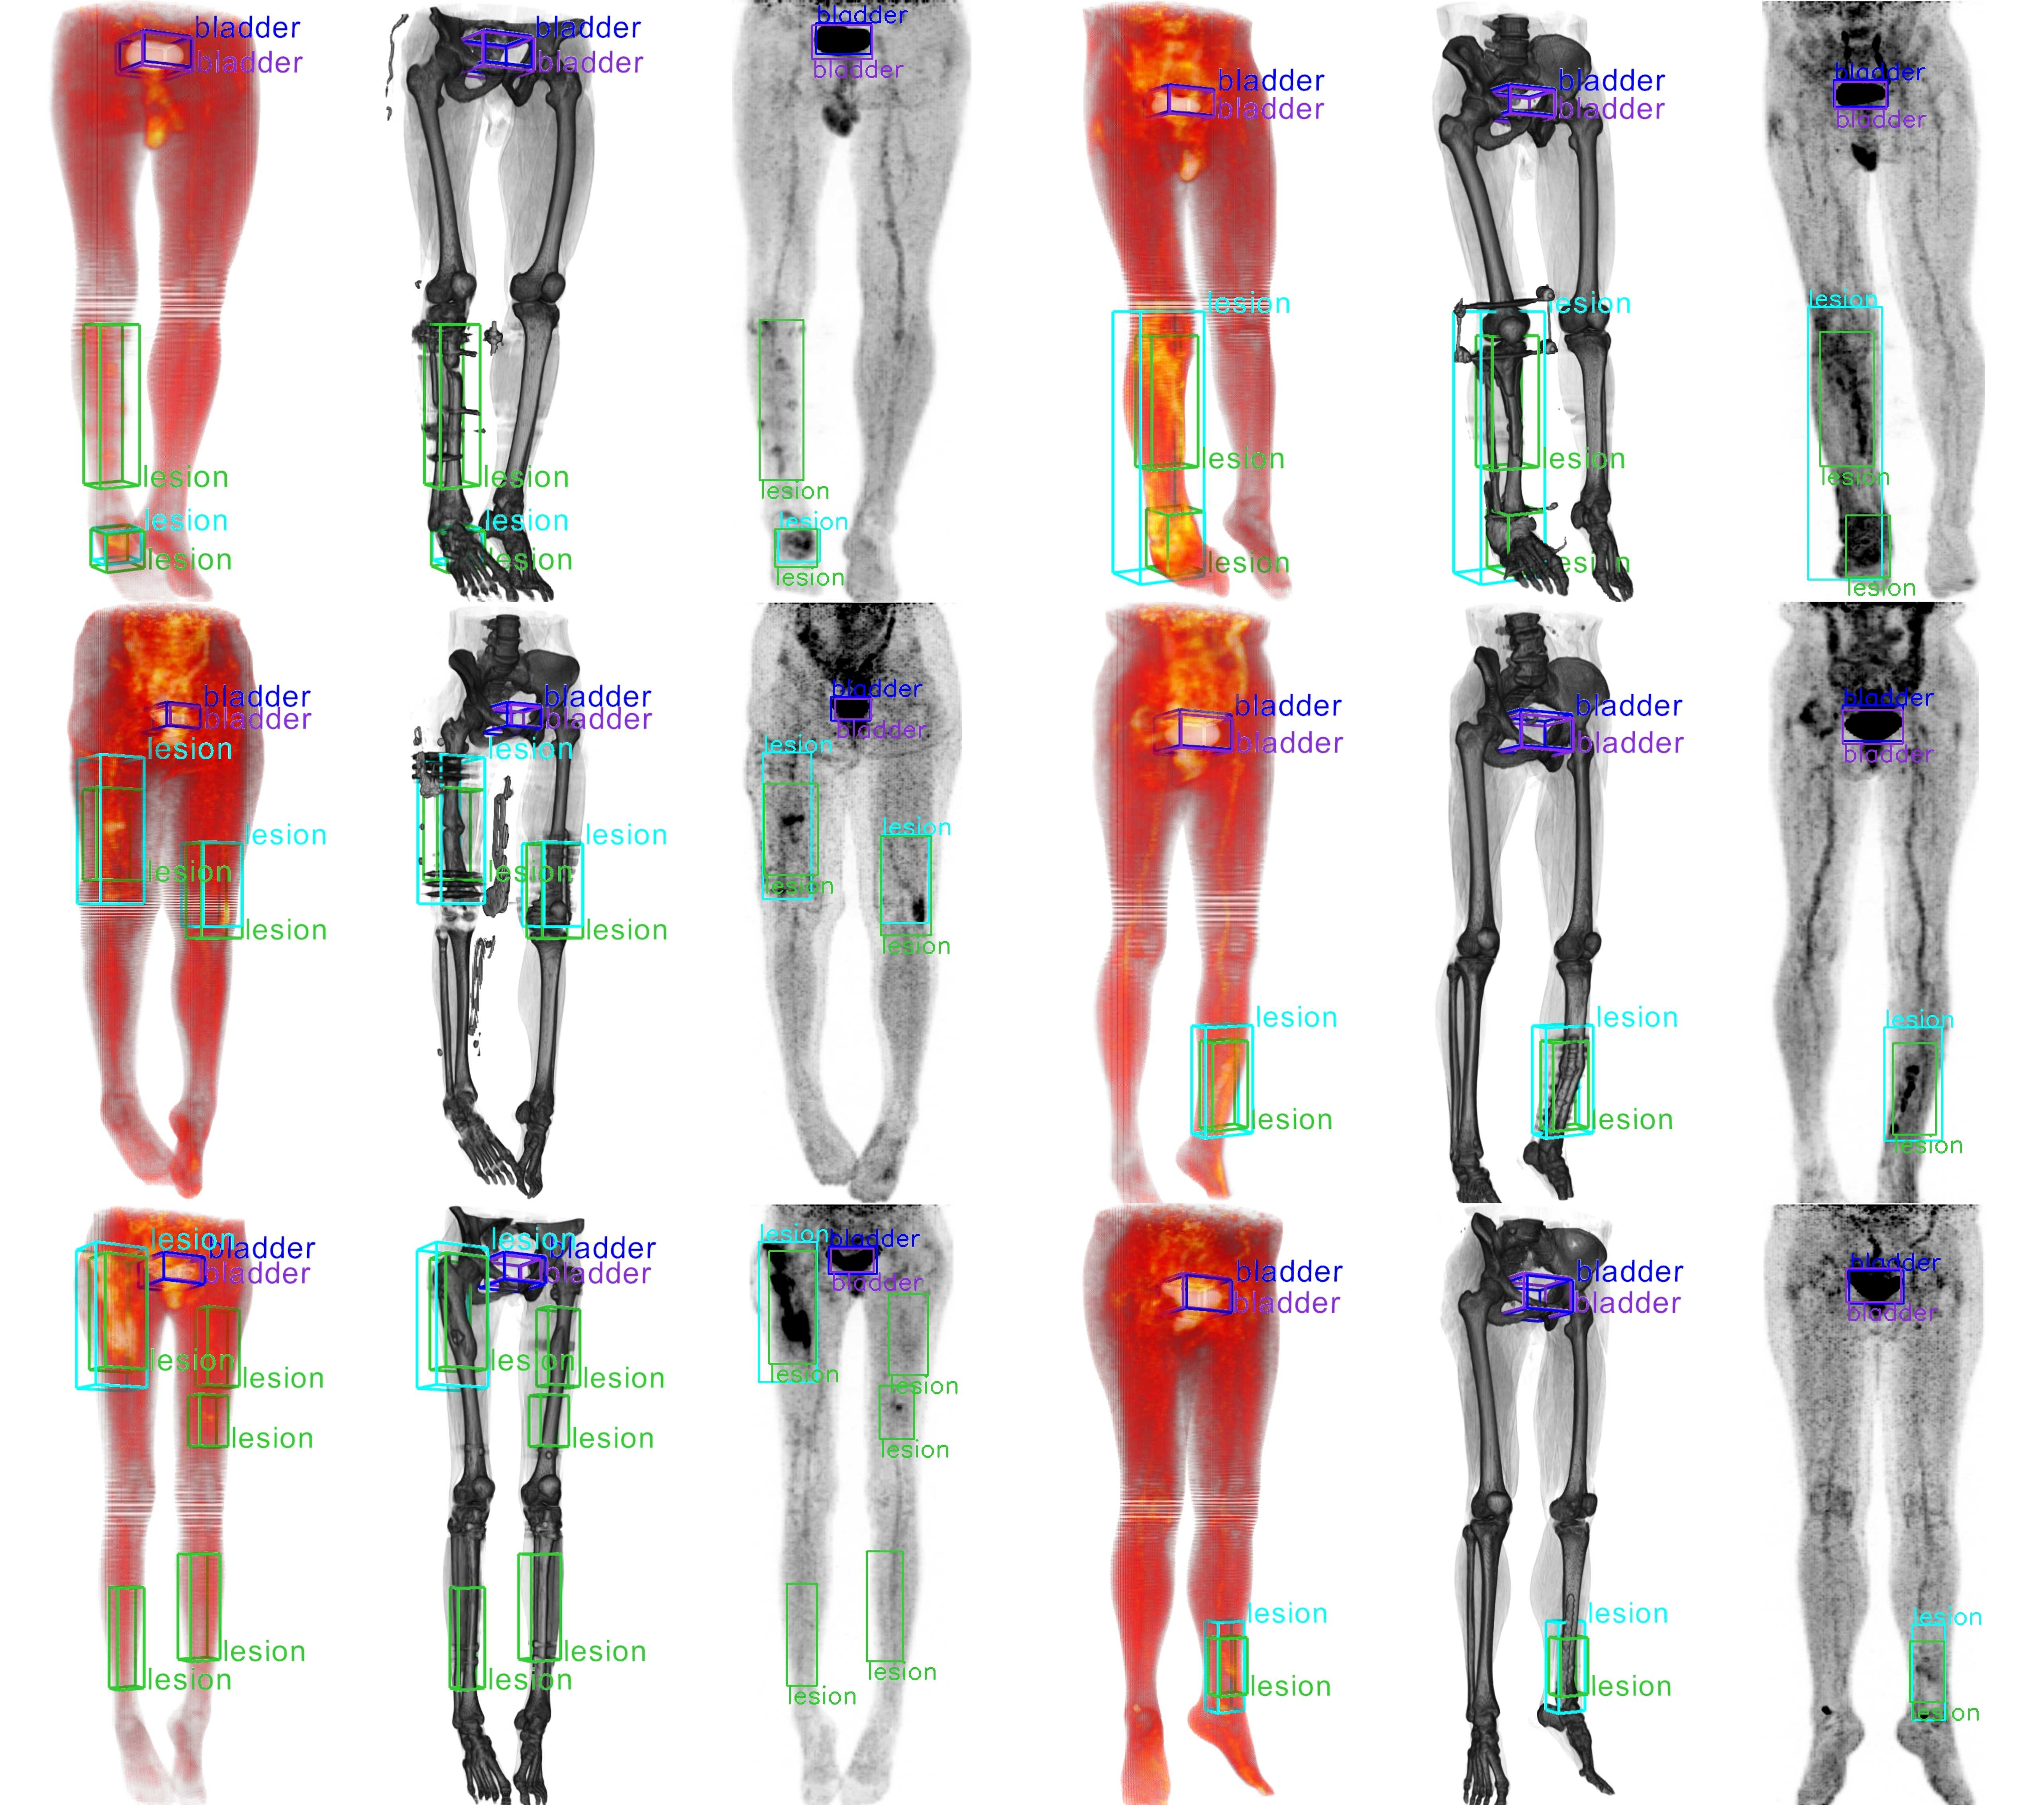
\includegraphics[width=\textwidth,height=\textheight,keepaspectratio]{figures/chap04_vis.jpg}
  \caption{322-YOLO检测结果的可视化图:每个患者有最大强度投影图像(PET),点云(3D PET)和三维重建的CT。青色和蓝色表示真实标签,紫色和绿色表示检测结果}
  \label{fig:chap04_vis}
\end{figure}

如图\ref{fig:chap04_vis}所示,322-YOLO展现了出色的性能,不仅能够准确定位已标注的病灶区域,而且能够有效检测出未标注的病灶区域(第1行第1列,第3行第1列)。特别值得注意的是,在病灶区域过大的情况下,322-YOLO还能通过使用两个边界框(第1行第2列)精准地定位病灶中更值得关注的子区域。此外,无论PET图像中是否存在高摄取区域,或者CT图像中是否存在骨侵蚀、骨折或内固定物等情况,322-YOLO模型都能够进行综合考虑并做出准确的检测与定位(第2行和第3行)。这表明了322-YOLO对于复杂场景和不同病变情况的强大适应性和鲁棒性。

\section{本章小结}

本章主要提出了一个基于\(^{18}\)F-FDG PET/CT影像的两阶段的下肢骨折相关感染病灶检测诊断分类网络框架3DFRINet,由预处理、322-YOLO病灶检测网络和ConvNeXt-S病灶诊断分类网络组成。预处理通过去除掉无关区域保留人体区域的PET SUV和CT HU输入到3DFRINet中。在322-YOLO病灶检测网络中,通过双分支主干网络结构设计与通道注意力模块有效地提取并融合三维PET的生理代谢信息和CT的解剖结构信息,从而充分利用不同模态的特点准确地检测病灶。通过最大强度投影将检测到的病灶从三维转换为二维,在降低数据和模型规模的同时获取有效特征,ConvNeXt-S病灶诊断分类网络达到了优异的分类性能。在下肢骨折相关感染的诊断任务中,该框架在检测方面达到了0.9234的AP\(_{25}\)和0.3041的AP\(_{50}\),在诊断分类方面达到了91.55\%(83.10\%,97.18\%)的准确率、0.9250(0.8533,0.9756)的F1和0.9331(0.8547,0.9870)的AUC,这表明该框架具有优越的病灶检测性能和良好的诊断分类性能。在与核医学医师的比较中,该框架相当或优于初级核医学医师,且与高级核医学医师相当。这进一步表现了深度学习方法在诊断假体关节感染的可行性与该病灶检测诊断分类网络框架的有效性。
% !Mode:: "TeX:UTF-8"
\chapter{骨科相关感染的自动诊断与可视化方法}

第三章和第四章分别详细地介绍了应用于动态骨显像和PET/CT中以人工智能为基础的假体关节感染辅助诊断框架和骨折相关感染辅助检测诊断框架。由于这两个框架无法提供便利且直观的辅助诊断以及可视化,本章继续在这一研究方向上深入,结合这两种人工智能方法并采用最新的PyQt6框架,去设计一种新颖的骨科相关感染的自动诊断与可视化方法。该方法旨在构建一个骨科相关感染的自动辅助诊断全流程,提供全面的医学影像可视化、阅览和分析功能,以促进临床诊断中假体关节感染与骨折相关感染的诊断决策和提高准确性。

\section{问题分析}

在设计假体关节感染和骨折相关感染的自动诊断与可视化方法时,必须深入考虑核医学专家在诊断这类骨科相关感染疾病的具体流程和对医学影像的可视化需求。这一方法需要融合多种先进的图像处理技术,同时也要求透彻地理解并仿真医生的诊断流程。这要求此方法不仅要精确处理和展示医学影像,还具备医学的决策智能,以提供直观、准确的诊断辅助。因此,本章主要包含以下两个方面的研究:

(1)模拟核医学医生的诊断流程。在假体关节感染和骨折相关感染诊断任务中,核医学专家遵循的实际临床诊断流程具体包括:首先,在动态骨显像或PET/CT中,精确定位到潜在的病灶区域。随后,核医学专家依靠专业的工具对所定位的病灶区域进行深入的分析和评估。最后,核医学专家将依托其丰富的临床经验和细致的视觉评估作出最终的诊断决策。

由此,在本章中,所研究的自动诊断方法需要集成第三章和第四章设计的图像处理技术。这些图像处理技术能够从复杂的动态骨显像和PET/CT影像中提取到关键的生物标志物,通过端到端地方式直接在医学影像中进行辅助诊断。特别是第三章采用了CNN和ConvLSTM,用于深入地学习动态骨显像中的图像特征和序列变化,这对于髋关节和膝关节假体感染的准确诊断至关重要。同时,第四章利用基于深度学习的检测和分类算法处理PET/CT影像,以获得更加全面立体的解剖结构和生理代谢信息,进而有效地锁定病灶区域,并对骨折相关感染进行精准诊断。

(2)不同医学影像模态的可视化。在核医学专家的临床诊断流程中,不同医学影像的可视化是最基础的需求之一。可视化需要能够处理、解析和展示不同来源的影像数据,如动态骨显像和PET/CT(PET SUV和CT HU),保证医生在做出诊断决策时能够全面考量所有相关影像信息。

由此,在本章中,所研究的可视化方法需要使得医学影像可根据专业医生的具体需求进行个性化调整,包括调整对比度、缩放、以及使用不同的着色方案以适应不同的医学影像模态和增强特定组织或病变的可视性等。同时,也需要特别注重和优化医生的视觉体验,提供直观的用户界面来展示各种各样的影像数据。通过提供分层视图、切换视图、融合影像和三维重建功能等,帮助医生从不同角度分析单一模态和多模态影像,从而得到更全面的诊断信息。

\section{总体设计}

本章设计了一个基于深度学习和PyQt6框架的骨科相关感染自动诊断和可视化方法,旨在提供精确地诊断辅助。如图\ref{fig:chap05_overall}所示的方法流程涵盖了四个关键模块和相应的工作流程。整个方法流程由四个主要步骤构成:

\begin{figure}[h]
  \centering
  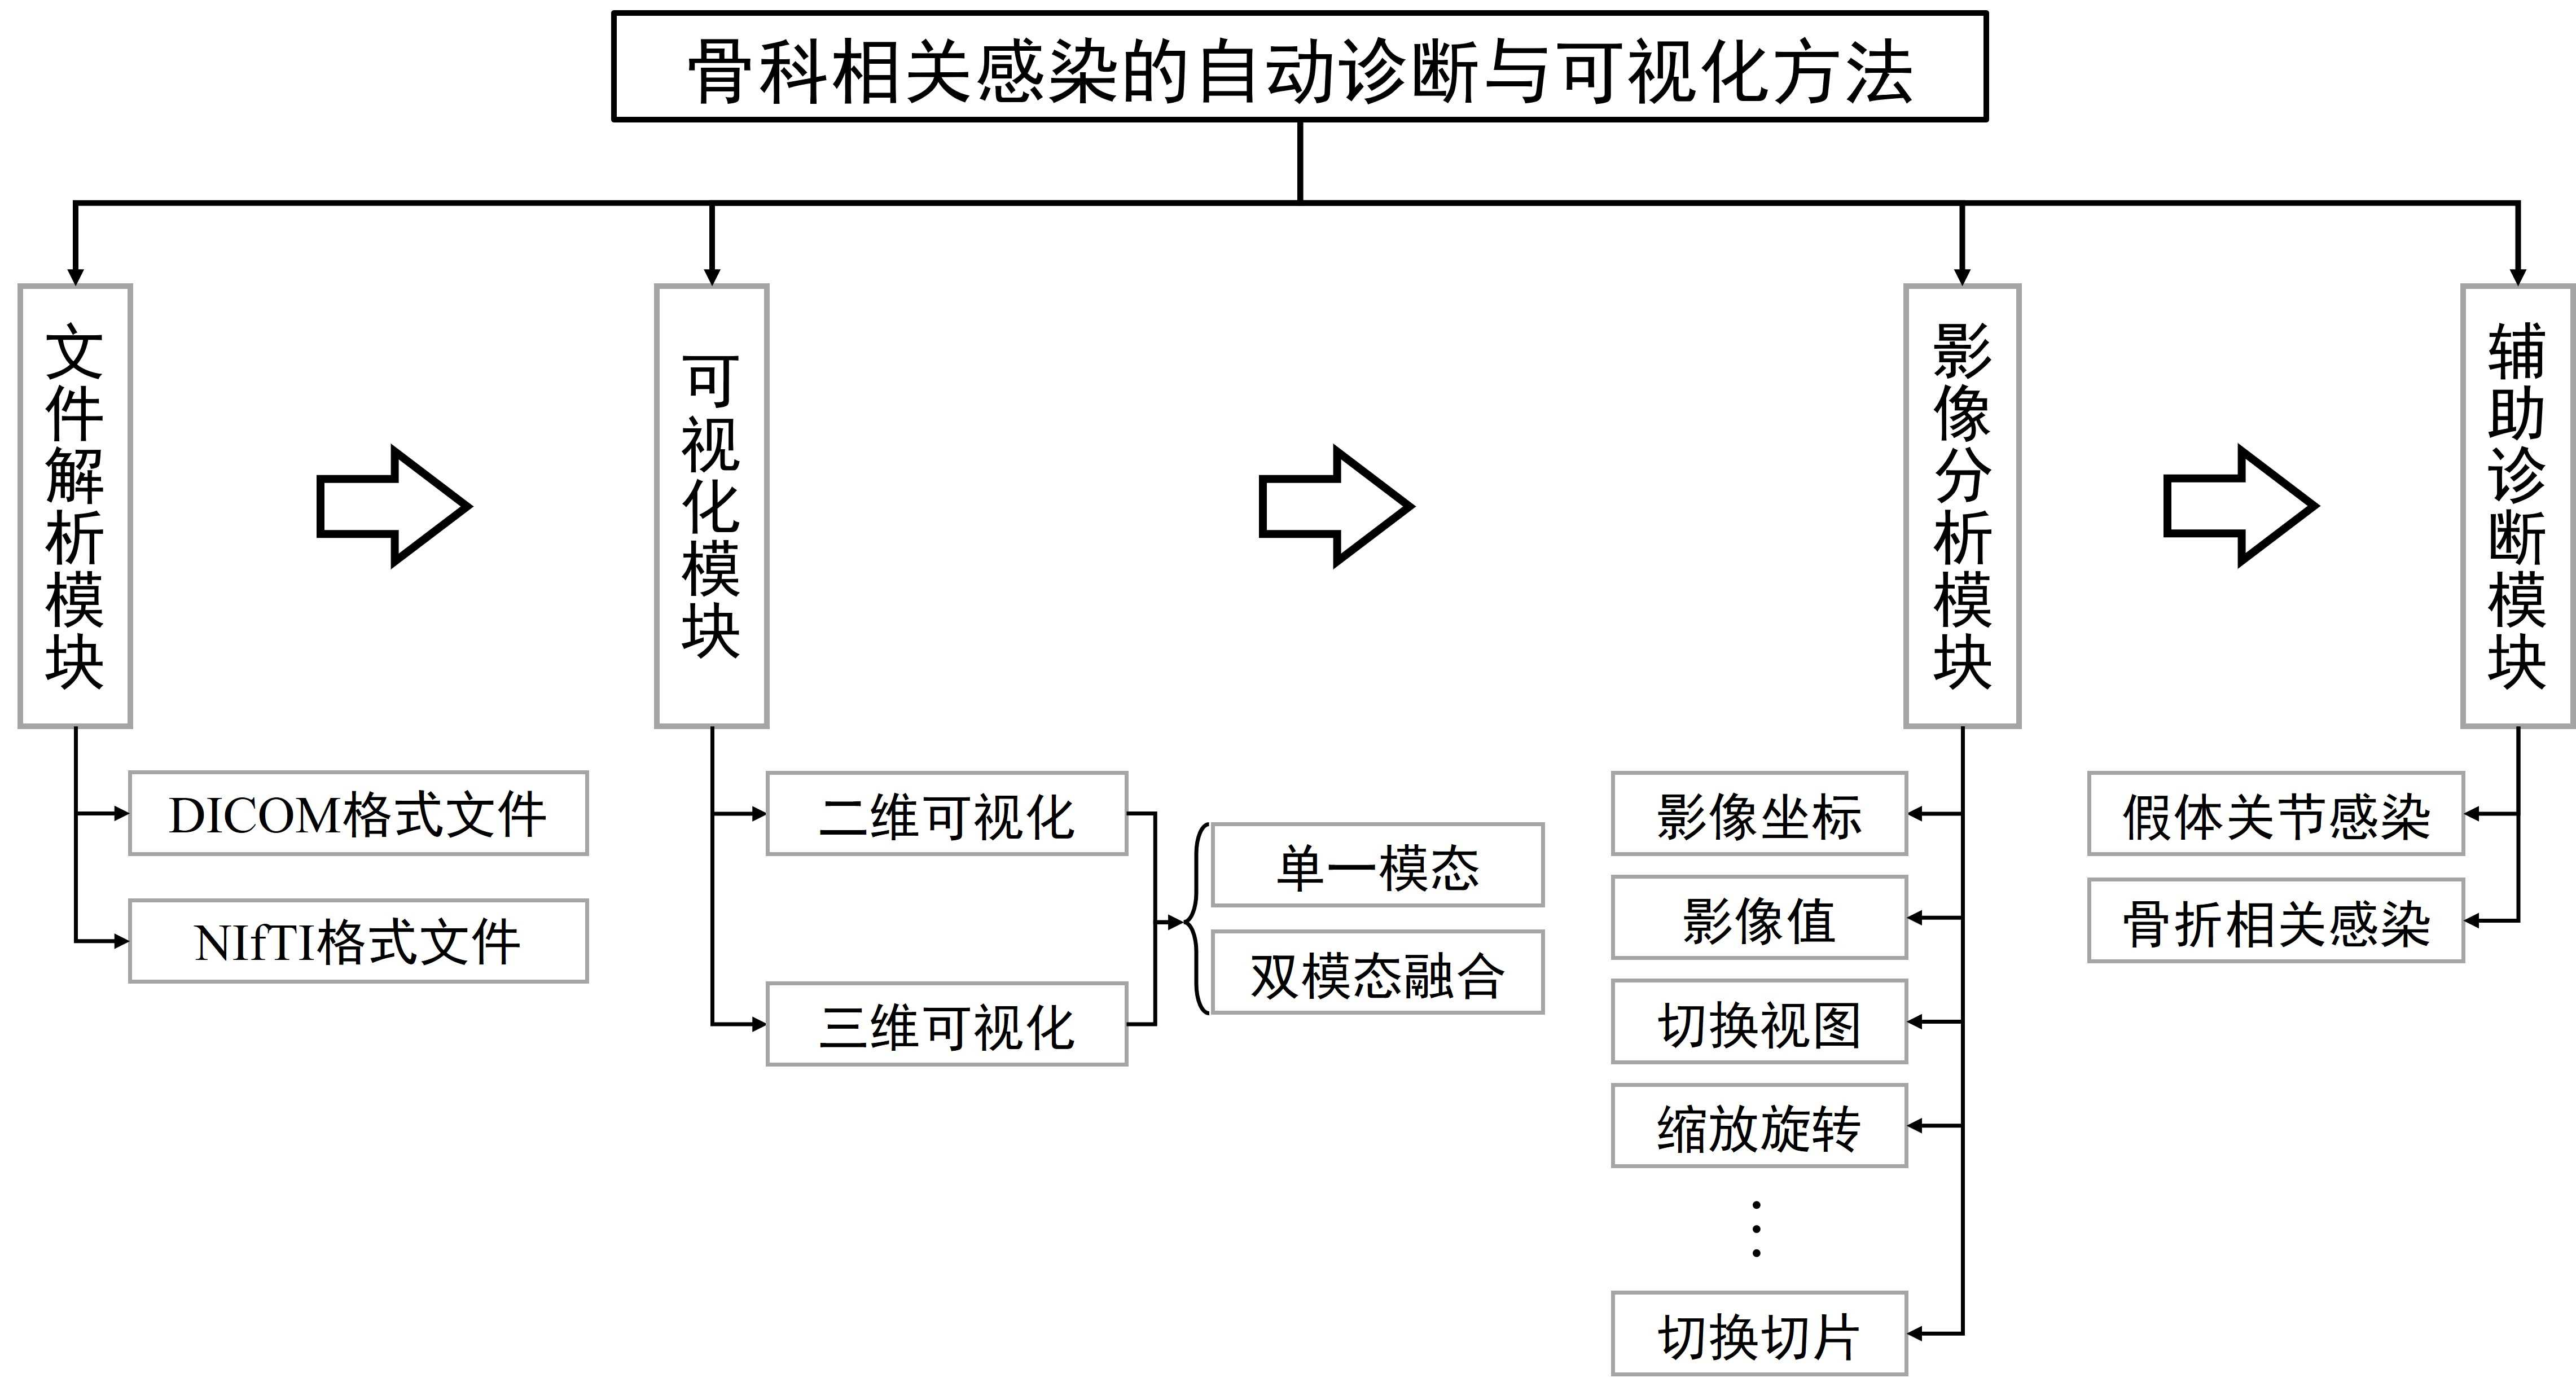
\includegraphics[width=\textwidth]{figures/chap05_overall.jpg}
  \bicaption{总体设计}{Overall design}
  \label{fig:chap05_overall}
\end{figure}

\begin{enumerate}
  \item 文件解析:被用户选定的DICOM或NIfTI文件经过读取和解析,其中根据各自的文件规范执行相应的解码流程,旨在准确抽取所需的医学信息数据。
  \item 可视化:经过解析得到的数据在预处理后转化为视觉表现形式,以直观展示医学影像。该预处理包括标准化、配准和融合,以提供丰富且细致的视觉信息。
  \item 影像分析:在实现影像数据的视觉呈现后,影像分析步骤提供了一系列工具,用于在多个视角和尺度下观察医学影像,包括视图切换、仿射变换等等操作。
  \item 辅助诊断:在用户通过可视化和影像分析获得初步印象后,辅助诊断步骤通过第三章和第四章中描述的深度学习框架,为假体关节感染和骨折相关感染提供辅助诊断能力。
\end{enumerate}

从文件解析开始,DICOM和NIfTI格式的医学影像数据由文件解析模块进行读取与解析。DICOM数据由于其独有的详细性和医疗信息的丰富性,需要处理其复杂的元数据以提取诊断所需的重要数据;而NIfTI格式则常用于功能成像和三维影像处理,因此其解析旨在获取空间结构信息以便后续分析。

在完成解析之后,可视化模块将根据用户选择的医学影像数据和可视化功能进行相应的处理。该模块支持单模态和双模态影像的二维和三维可视化。在可视化过程中,医学影像数据均被默认设置为三维结构。对于原本是二维的医学影像数据,将自动扩展出一个大小为一的维度,以便与既定的三维数据结构保持一致性。因此,本章可视化模块的数据处理和分析侧重于三维及以下维度的医学影像。

影像分析模块根据用户的需求,对医学影像执行特定的操作。此模块功能广泛,包括展示影像坐标与在特定坐标上用于临床评估的影像值、切换不同视图,例如矢状面、冠状面和横断面、以及执行仿射变换操作等。每项功能都旨在为医生提供详细的医学影像信息,从而更准确地定位和诊断潜在的病灶区域。

最终,在完成医学影像的可视化以及初步分析后,辅助诊断模块融合了假体关节感染辅助诊断框架与骨折相关感染检测诊断框架,可以给用户提供医学辅助诊断建议。该建议包括在动态骨显像中对患者的膝部或髋部的假体进行诊断,以及利用PET/CT影像检测与识别患者下肢中潜在的感染区域。辅助诊断模块基于医学影像特征辅助医生评估病灶的性质以及严重程度,为医学诊断提供更高的准确性与效率。

\subsection{界面设计}

图\ref{fig:chap05_preview}呈现的是所设计的骨科相关感染的自动诊断与可视化方法的界面。界面主要分为侧边导航栏和中心的可视化显示区域。在侧边导航栏中,展示了DICOM和NIfTI文件由文件解析模块处理所得的层次化结构信息。该信息采用了可折叠的列表按钮的形式,详细地列出了患者的姓名拼音与影像扫描的具体时间,并在其内部展示了归属于当前患者的影像数据,例如系列描述与影像尺寸信息。侧边栏顶部设置了多个功能按钮,包括打开文件、删除已解析的影像数据、二维影像展示、三维影像展示、二维影像融合以及三维影像融合。其中,功能按钮将作用于侧边导航栏中被勾选的医学影像数据。

\begin{figure}[htbp]
  \centering
  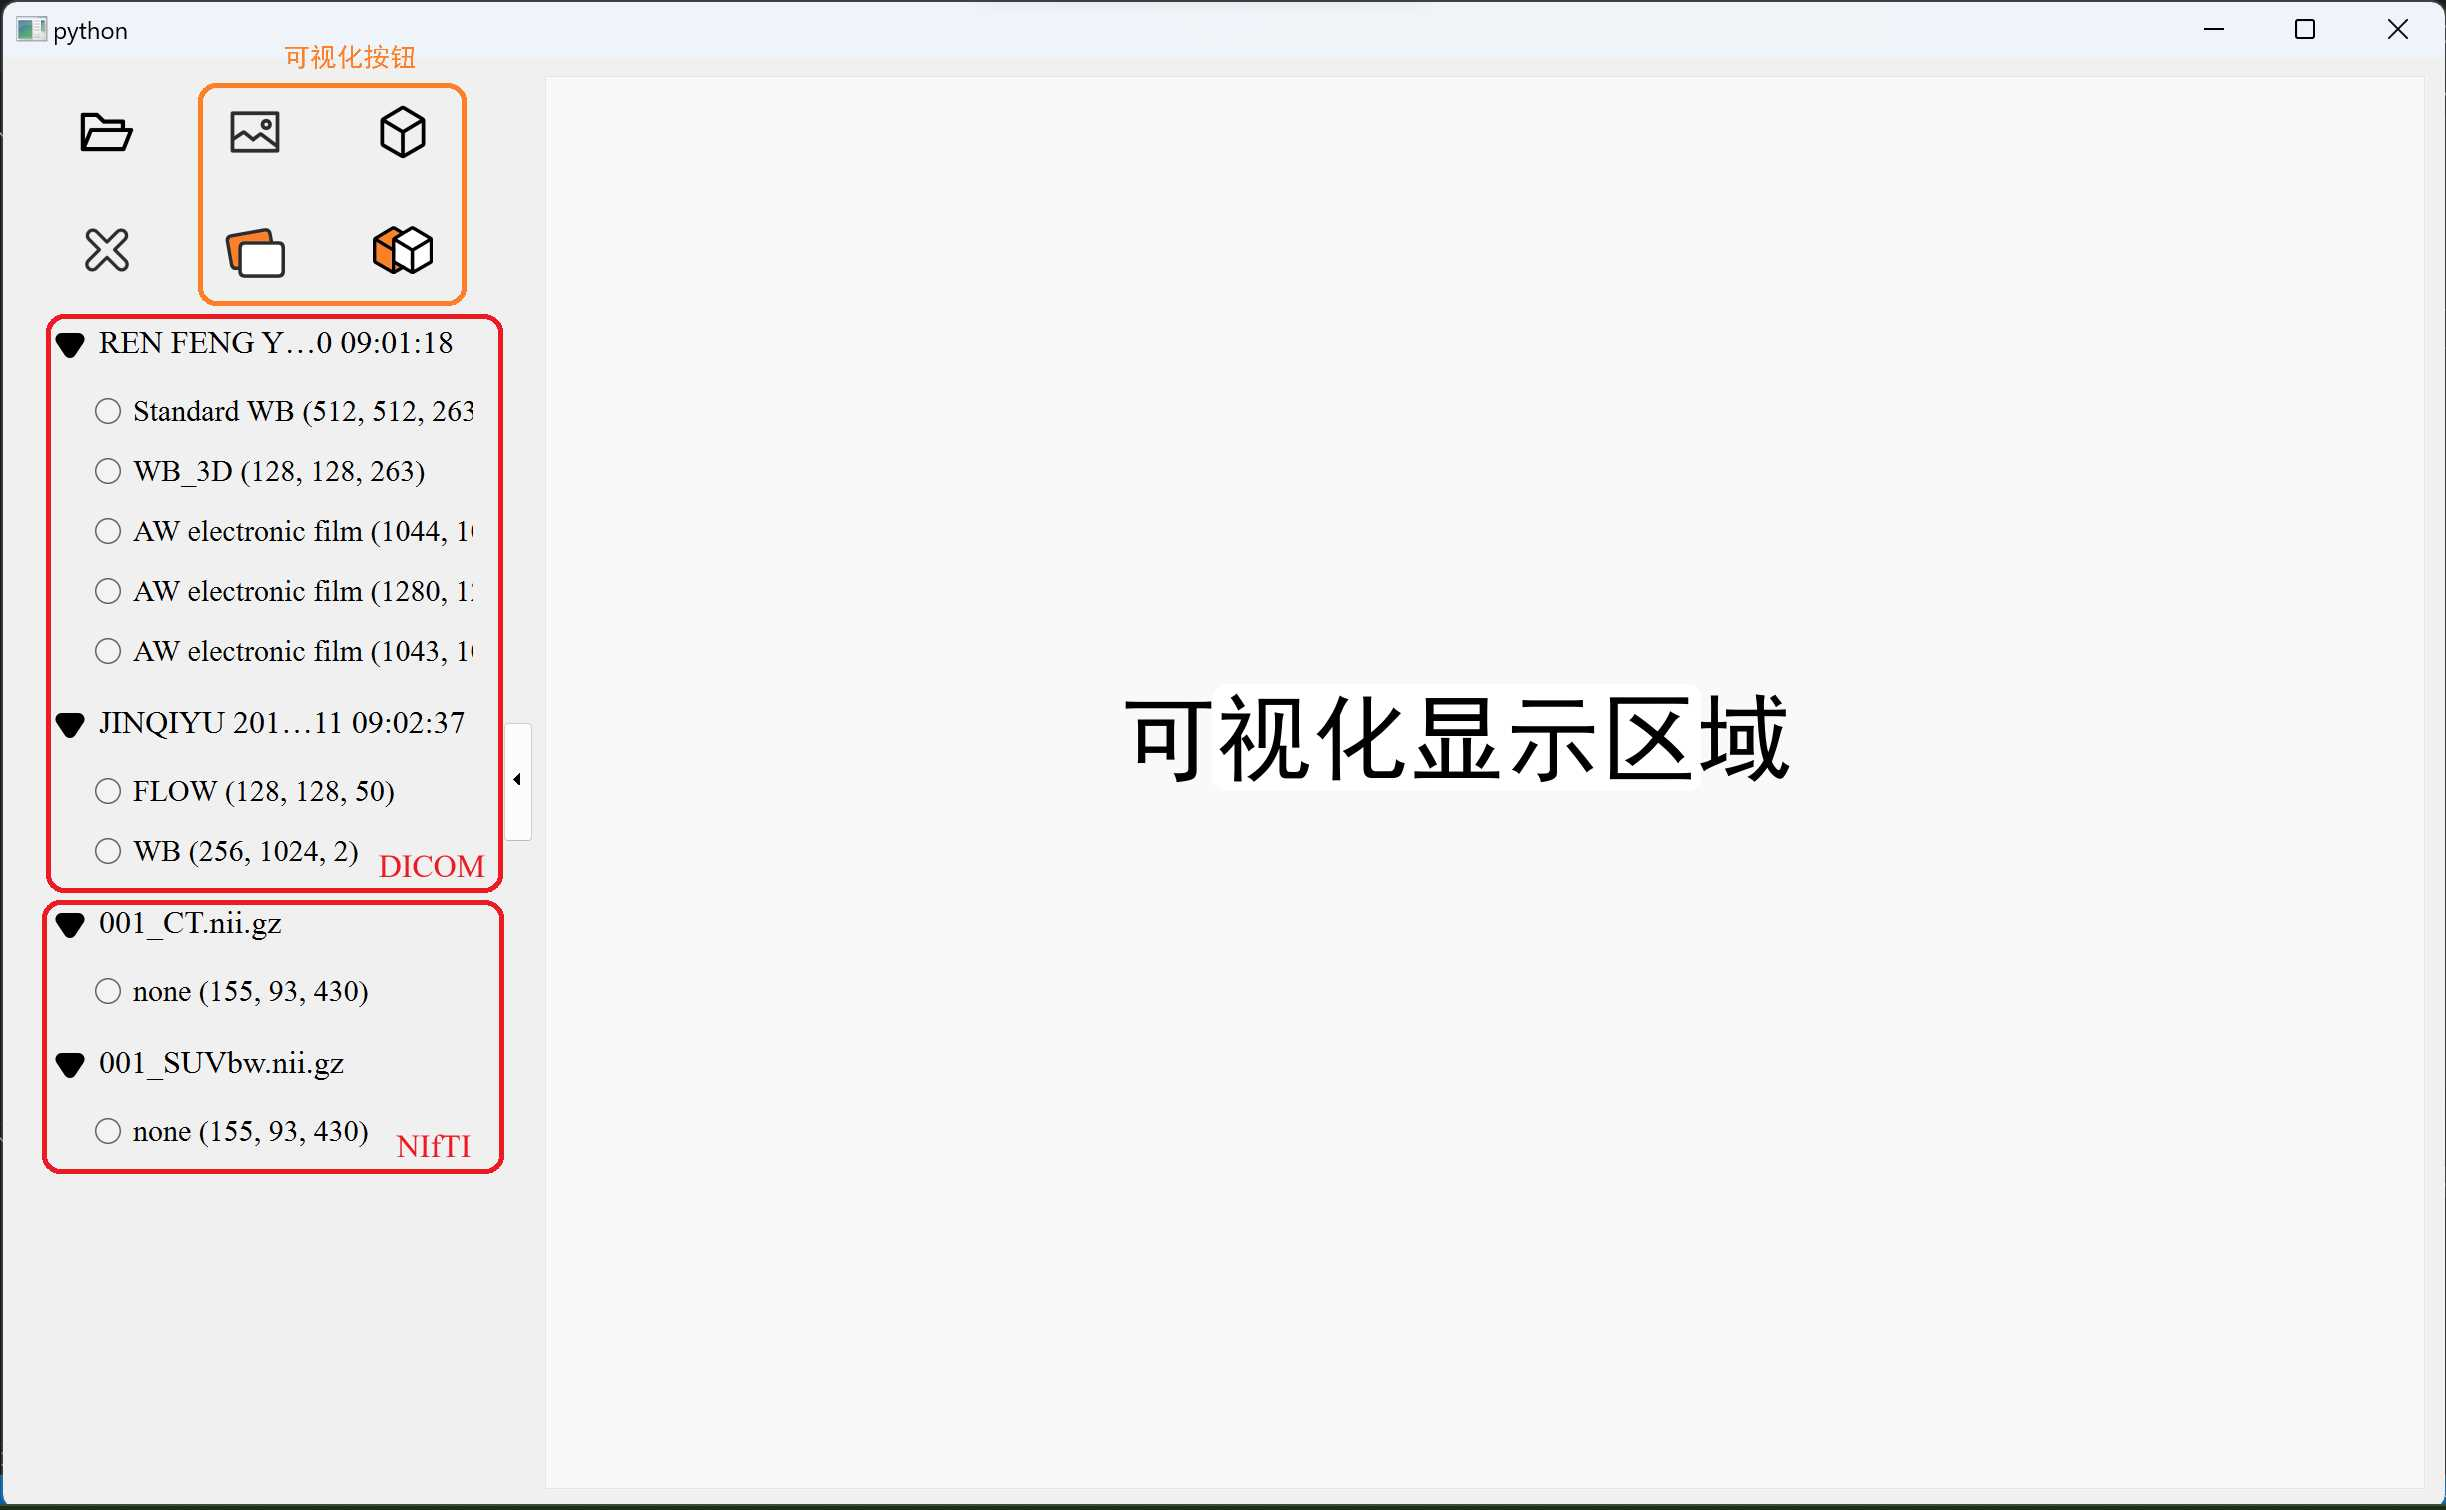
\includegraphics[width=\textwidth]{figures/chap05_preview.jpg}
  \bicaption{系统界面}{System interface}
  \label{fig:chap05_preview}
\end{figure}

中央的可视化显示区域将依据操作者在侧边导航栏中执行的操作,以标签页的形式对医学影像数据进行可视化显示。图\ref{fig:chap05_view}展示了四种不同可视化功能下每个标签页顶部配备的工具栏,其中融合了影像分析模块与辅助诊断模块的众多功能。

在影像的二维可视化中,工具栏前端不仅显示了当前视图信息,同时展示了位于可视化区域中心蓝色十字准星所指示的像素位置坐标及其相关的影像值,这些信息用于评估和分析至关重要。值得说明的是,坐标可以进行修改,可视化区域也会随之进行更新。工具栏包含了多种功能按钮:视图按钮用于变换不同的视角;操作按钮允许用户复原图像、执行旋转及进行镜像翻转;鼠标左键图标按钮则使用户能够通过鼠标左键拖拽影像或移动蓝色虚线十字准星;切换按钮则可以让鼠标滑轮的功能在切换切片和缩放之间进行转换;对比度按钮则用以调整可视化影像的对比度。此外,还包含了导入分割图像或者边界框的标签按钮,调节标签透明度的滑块,以及用于给出辅助诊断建议的AI按钮。

\begin{figure}[htbp]
  \centering
  \bisubcaptionbox{二维展示\label{fig:chap05_view_2D}}{2D display}[0.49\textwidth]{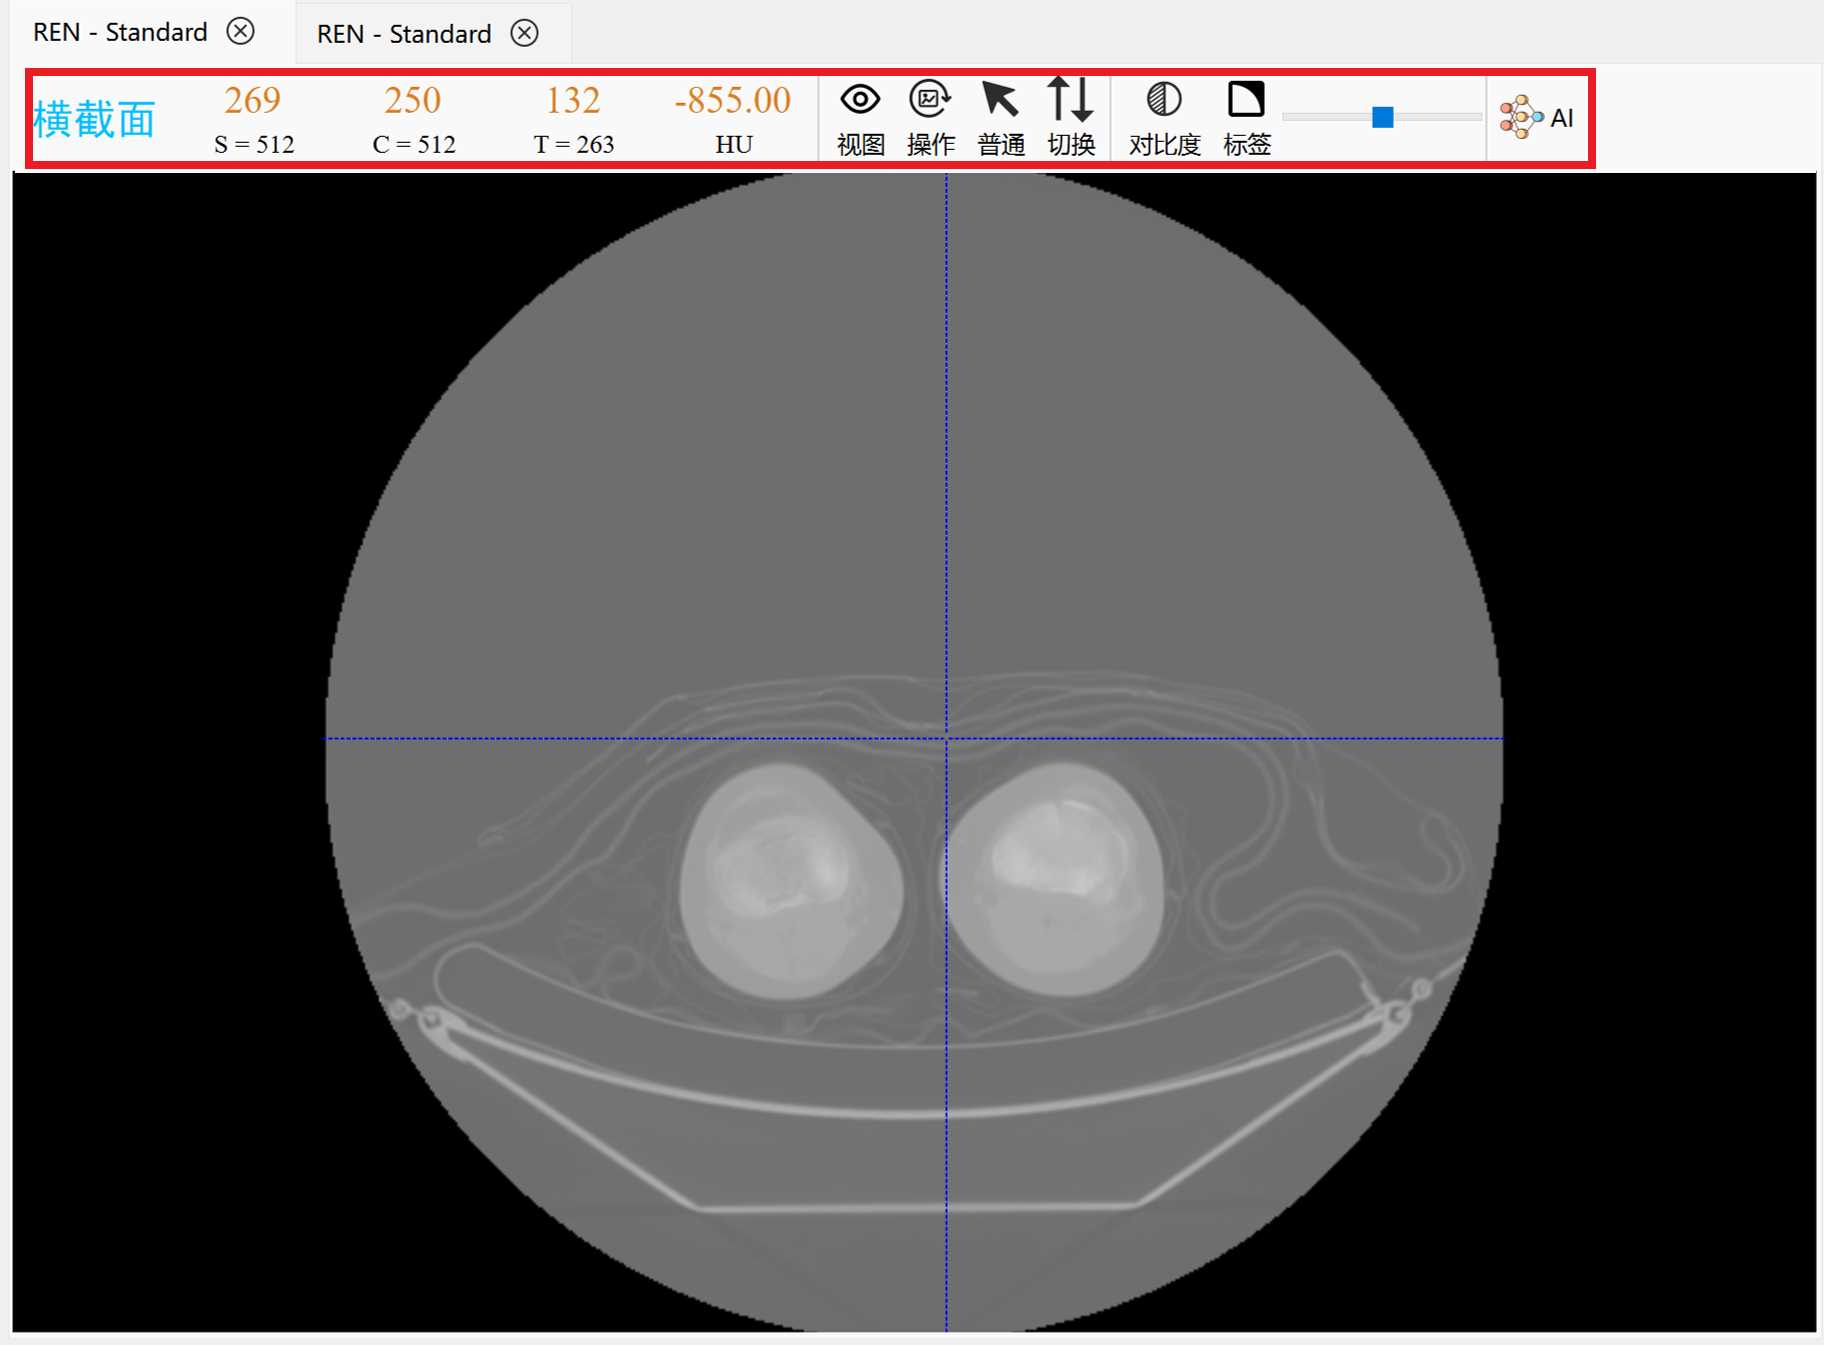
\includegraphics[scale=0.3]{figures/chap05_view_2D.jpg}}
  \bisubcaptionbox{二维融合\label{fig:chap05_view_2DF}}{2D fusion}[0.49\textwidth]{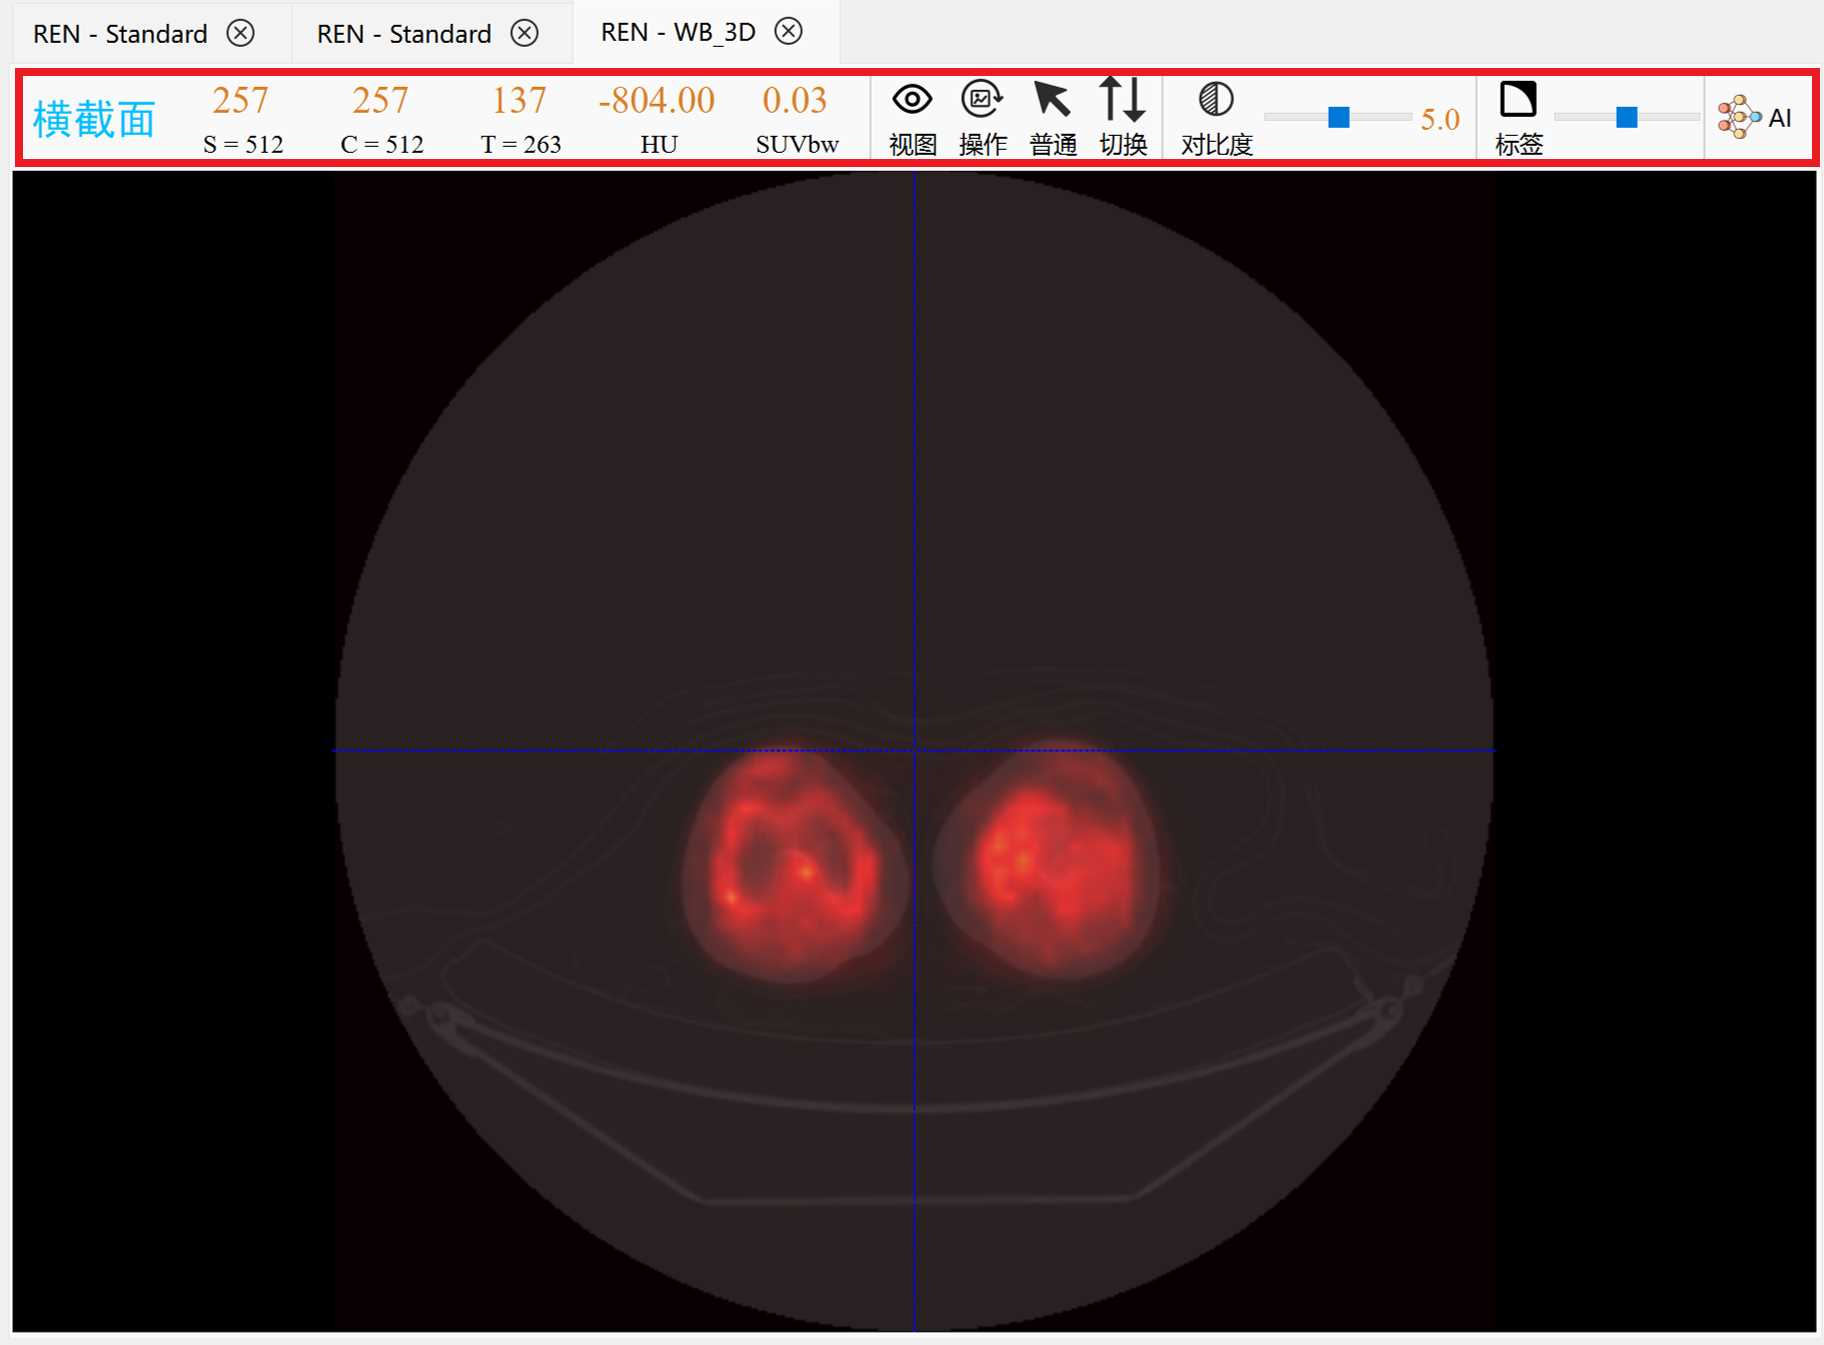
\includegraphics[scale=0.3]{figures/chap05_view_2DF.jpg}}
  \bisubcaptionbox{三维展示\label{fig:chap05_view_3D}}{3D display}[0.49\textwidth]{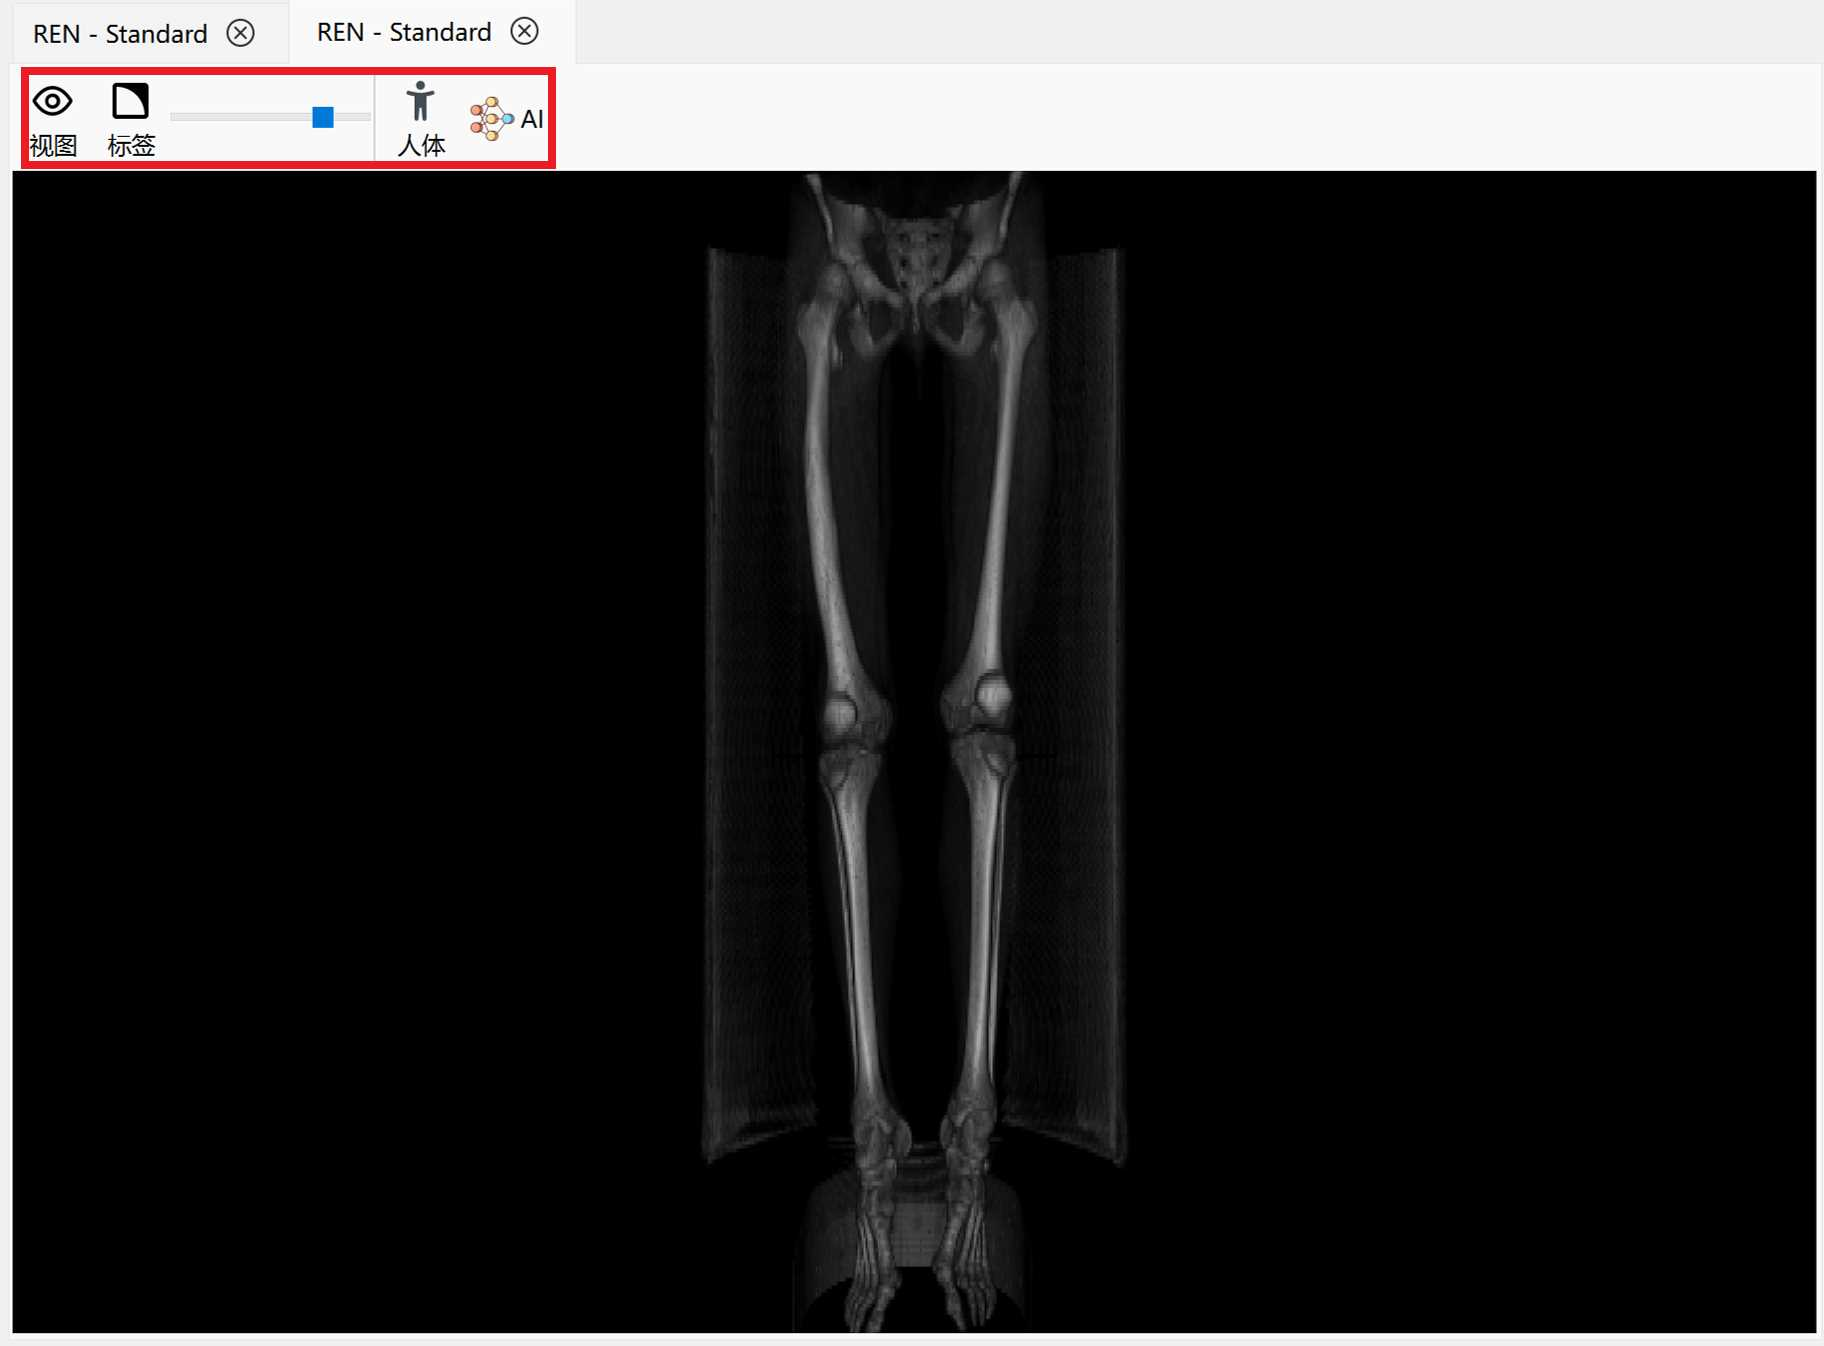
\includegraphics[scale=0.3]{figures/chap05_view_3D.jpg}}
  \bisubcaptionbox{三维融合\label{fig:chap05_view_3DF}}{3D fusion}[0.49\textwidth]{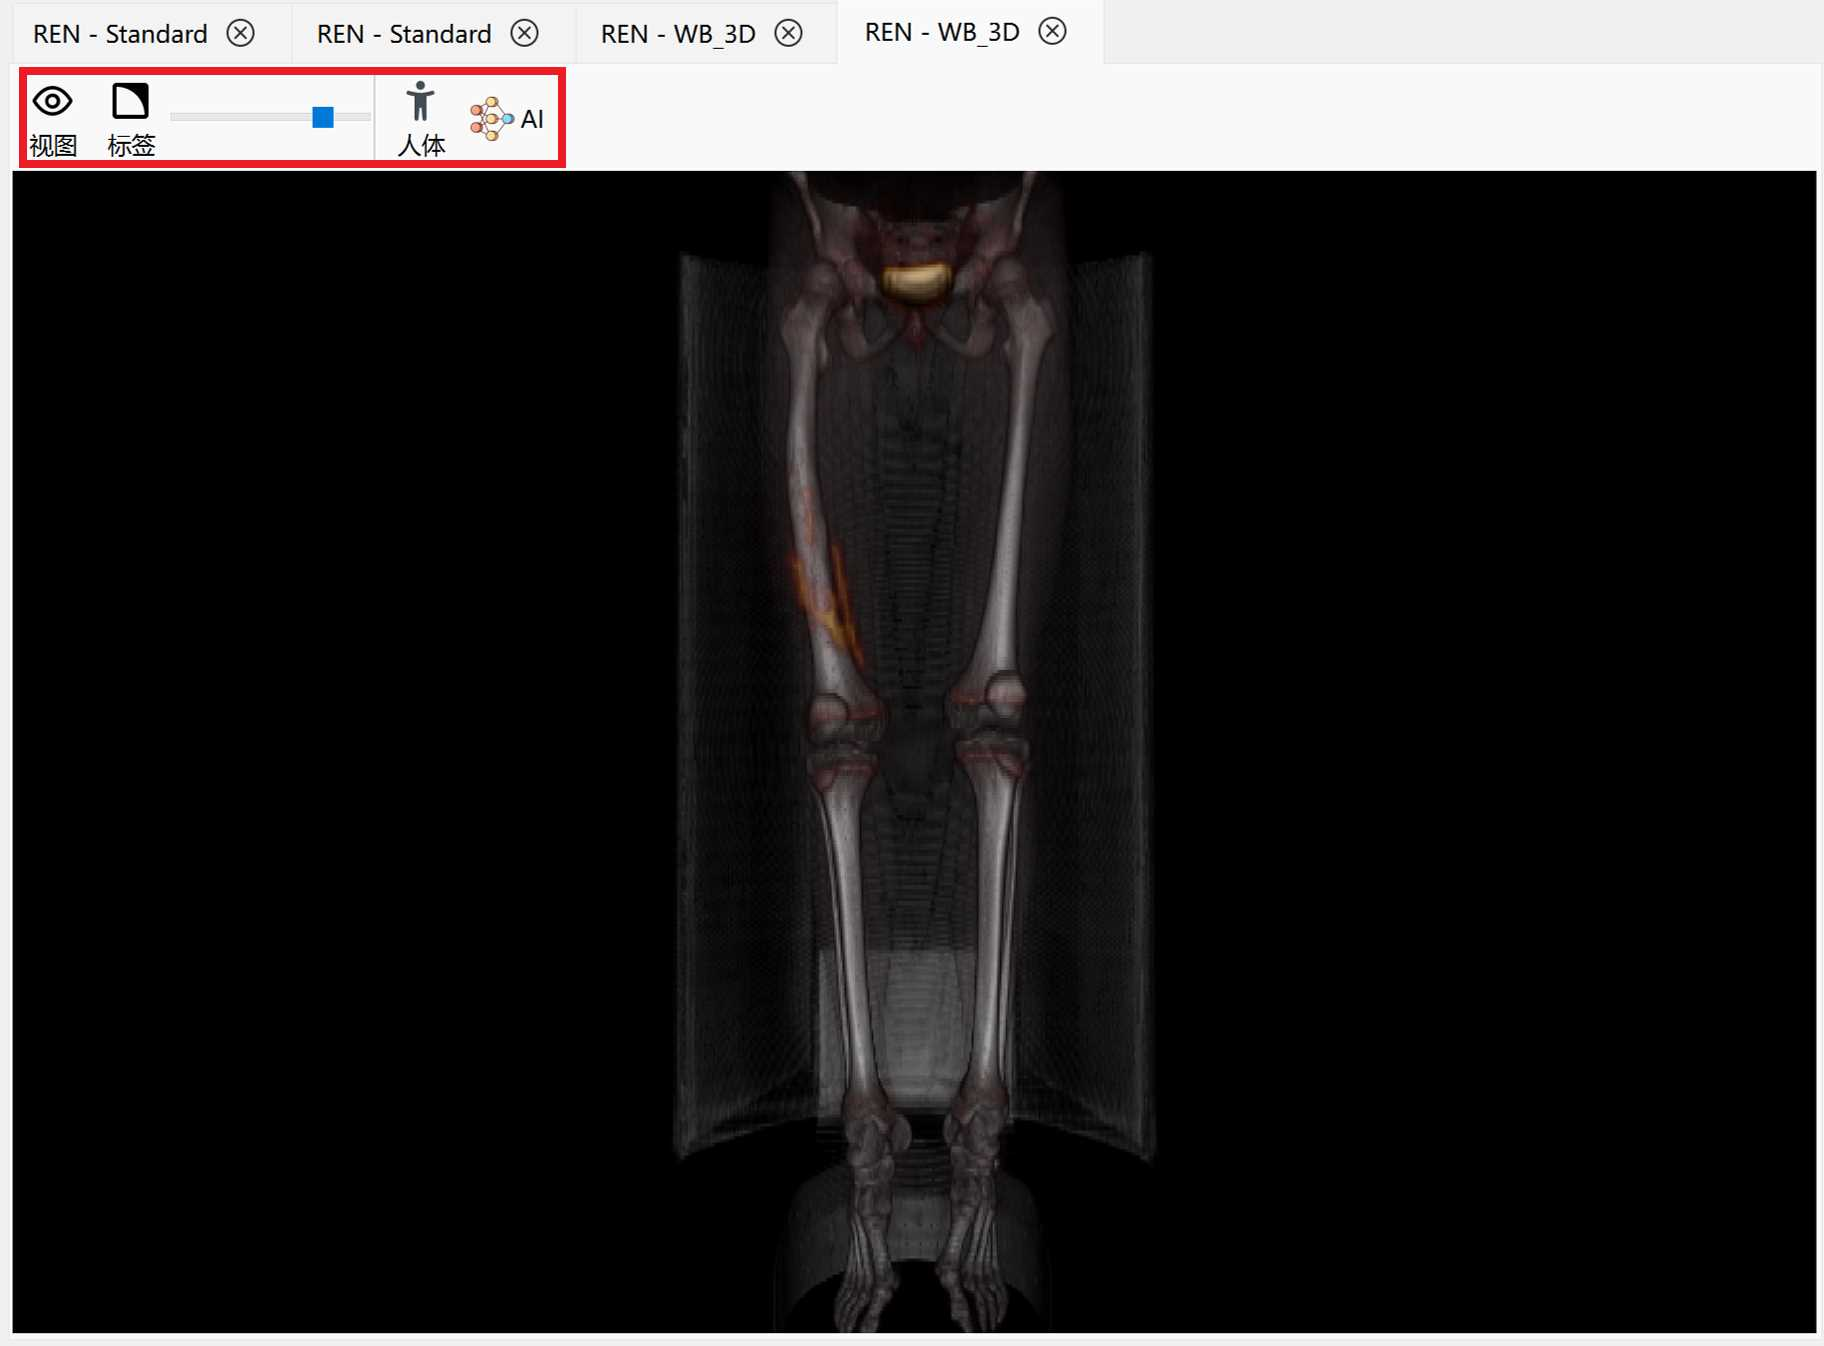
\includegraphics[scale=0.3]{figures/chap05_view_3DF.jpg}}
  \bicaption{可视化界面}{Visual interface}\label{fig:chap05_view}
\end{figure}

在影像的三维可视化工具栏中,视图功能按钮使用户能够选择展示整体影像数据或仅展示根据标签图导入的边界框所分割的部分;标签功能按钮方便用户导入标注病灶区域的边界框;透明度调节滑块通过精细控制,使得边界框标签透明度得以调整;而人体功能按钮则在PET/CT影像融合展示中,提供了移除机床视图的选项;同样地,AI按钮针对三维影像提供辅助诊断功能。此外,用户可通过鼠标左键操控,使影像围绕其几何中心在三维空间内进行旋转,而鼠标滚轮则赋予了以影像中心作为锚点进行放大或缩小的功能。

\section{自动诊断}

辅助诊断模块,作为本章研究中自动诊断方法的核心组成部分,集成了基于\(^{99m}\)Tc-MDP动态骨显像的假体关节感染辅助诊断框和基于\(^{18}\)F-FDG PET/CT三维影像的下肢骨折相关感染检测与诊断框架。在用户界面上,该集成的自动诊断方法通过一个简洁的AI按钮呈现于标签页的顶部工具栏中,从而在可视化显示区域中直观地提供使用接入点。

\subsection{辅助诊断模块}

通过简单地点击AI按钮,辅助诊断模块便可迅速触发内嵌的深度学习算法,进而自动对当前可视化的医学影像进行分析。特别地,辅助诊断模块会从医学影像的元数据中自动提取关键信息,以确保算法的适用性。算法开始对影像数据进行深入分析时,将对病灶区域进行精准的辅助诊断,并以可视化的方式展现出来。

\begin{figure}[htbp]
  \centering
  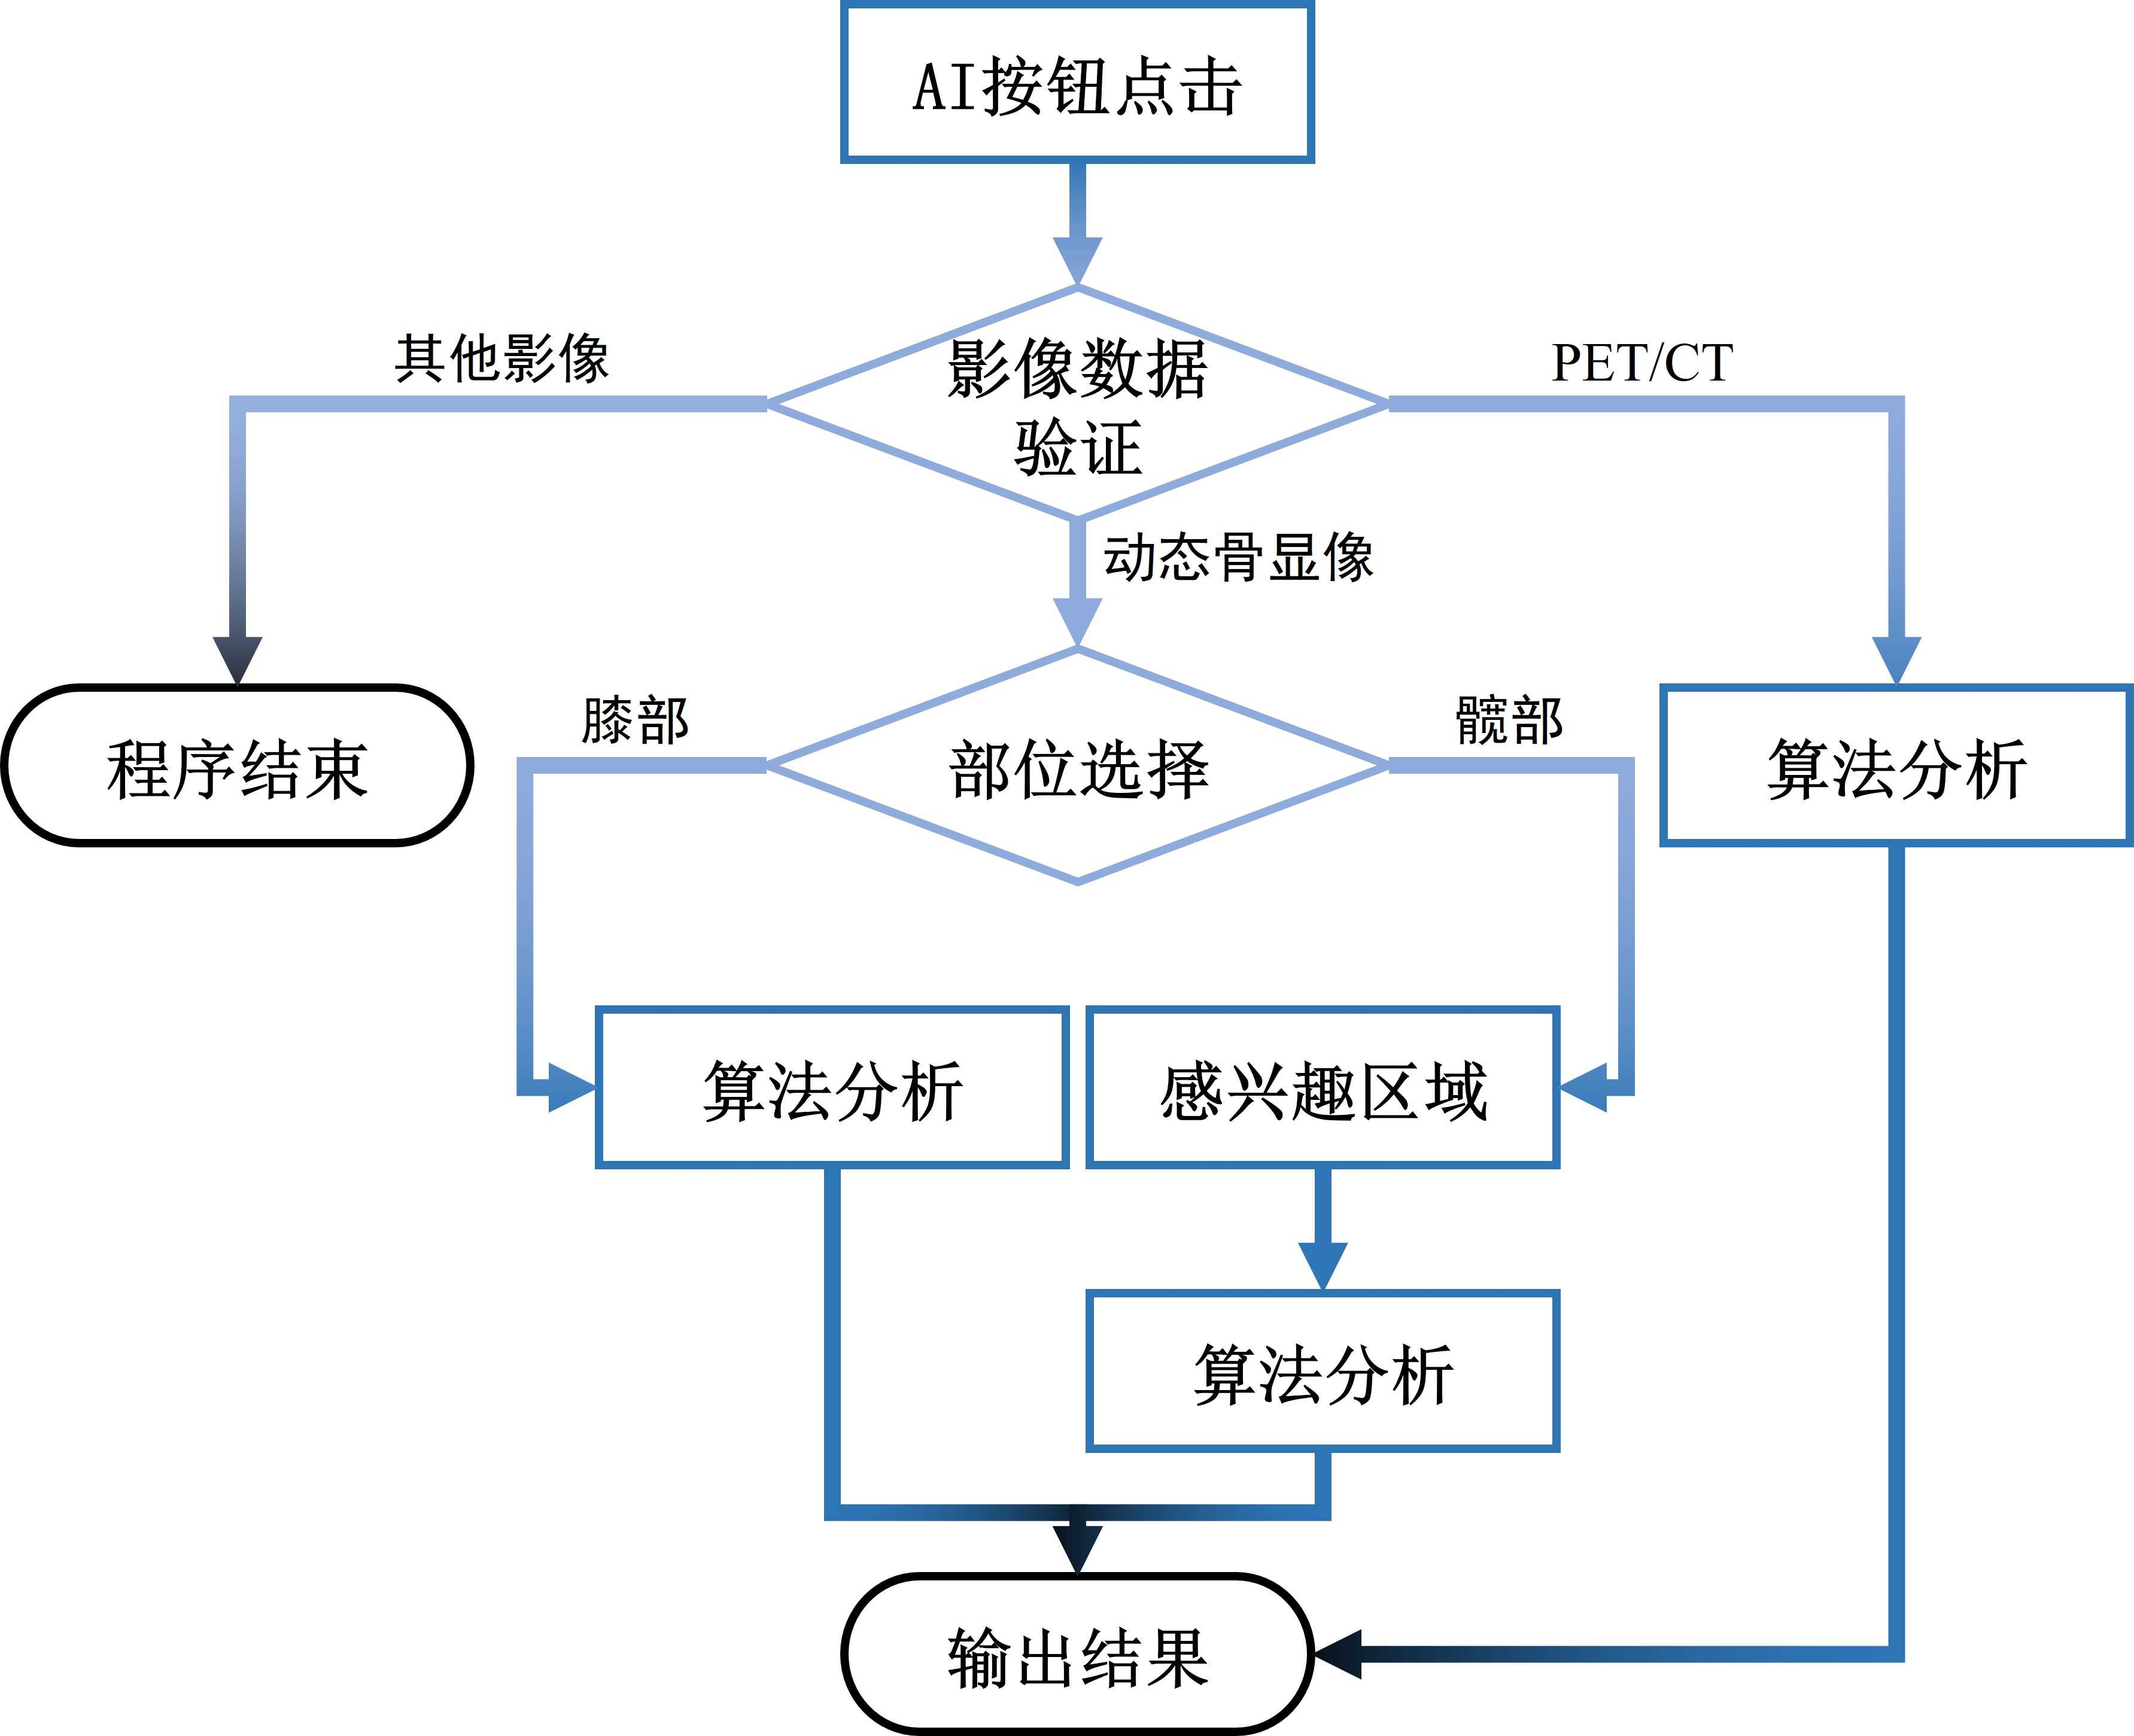
\includegraphics[width=0.75\textwidth]{figures/chap05_diagnose.jpg}
  \bicaption{辅助诊断模块的运行流程}{The processing flow of the auxiliary diagnosis module}
  \label{fig:chap05_diagnose}
\end{figure}

图\ref{fig:chap05_diagnose}展示了辅助诊断模块的整体运行流程。在初始阶段,对医学影像的元数据进行解析,从而识别所可视化的影像的模态。当遇到不兼容的影像模态时,辅助诊断模块会通过信息框提示用户,流程于此终止。

若影像模态确认为动态骨显像时,则会引导用户在膝部和髋部之间进行选择。选定膝部后,辅助诊断模块会立即采用第三章的框架,执行病灶的辅助诊断,同时通过计时弹窗提示程序正在运行中以及运行时间。髋部选择路径稍有不同,流程会进入一个选择感兴趣区域的环节。用户通过鼠标左键按下生成一个\(40 \times 40\)的红色边框,并在可视化区域中移动到理想的区域。随后,释放鼠标左键,辅助诊断模块将以鼠标位置为中心的\(40 \times40 \)的区域设置为感兴趣区域并提供给第三章的框架用于进一步分析和诊断。

若影像模态确认为PET/CT时,辅助诊断模块会自主调用第四章的检测诊断框架,开始识别和评估潜在的病灶区域,同时通过计时弹窗提示用户。在算法运行结束后,辅助诊断结果不仅以弹窗的形式对用户进行提示,同时在PET/CT中绘制出特定的边界框标注,从而实现了一个高效、直观且用户交互性强的辅助诊断工作流。

\section{可视化}

在本章研究中,可视化方法发挥着至关重要的作用,其由文件解析、可视化以及影像分析三大关键功能模块构成。文件解析模块构成了可视化方法的基石,它的主要职责在于解析影像文件数据,并将其重塑为三维医学影像,为之后的展示与分析奠定重要基础。可视化模块则构成了可视化方法的核心,该模块负责将解析后的医学影像数据转化并映射至自然图像领域中常规应用的色彩空间,其目的是提高影像的可读性的同时,使得医学影像的关键信息在视觉上更加明显。最后,影像分析模块代表了可视化方法的进阶扩展,它操控着对视觉呈现的医学影像的进一步图像处理,如调整对比度和缩放等。此模块便于用户进行细节分析,包括识别和解读影像上的关键特征,从而全面地挖掘影像所蕴含的深层次信息。

\subsection{文件解析模块}

在初始阶段,文件解析模块会将医学影像中原始的像素值转换为更适合用于评估和分析的影像值,用以确保了影像信息的临床相关性,还为后续的量化分析提供了定量的指标。例如,CT影像中原始像素值被转换成HU,PET影像的原始像素值则被转换为SUV。

对于DICOM文件,解析过程如下:
\begin{enumerate}[1)]
  \item 读取需解析的DICOM文件所在路径下的所有DICOM文件。
  \item 根据元数据中的Study Instance UID将这些文件划分到不同的研究组中。
  \item 根据元数据中的Series Instance UID进一步在研究组中划分为不同的系列组。
  \item 根据每个文件的影像大小,在系列组中再进一步划分为不同的尺寸组。
  \item 根据元数据中的Slice Location或Instance Number对尺寸组中的文件进行排序。
  \item 依次将每个尺寸组的文件组成一个完整的医学影像,并转换像素值为影像值。
  \item 数据以研究组、系列组、尺寸组和医学影像为顺序的层次化结构进行展示。
\end{enumerate}

在NIfTI(Neuroimaging Informatics Technology Initiative)文件的解析过程中,由于这类文件并不包含像DICOM格式那样丰富的元数据,因此其解析过程相对简单。解析一开始是读入NIfTI文件,并为之分配随机生成的Study Instance UID与Series Instance UID。接着读取该文件中的影像数据并获取影像大小。最终解析后的数据将按照一种与DICOM相同的层次化结构进行呈现。

\subsection{可视化模块}

在文件解析结束之后,可视化模块将对不同模态的医学影像数据采取差异化的可视化处理策略,具体可分为二维和三维两个维度,各自又包含单一模态展示和双模态融合展示两种处理方法。

对于二维展示,为了将医学影像值有效地映射到自然图像领域中的RGB色彩空间,可视化模块采用了最大最小值归一化方法,确保医学影像值可以在保持其诊断信息的同时,以一种标准化且用户直观理解的视觉形式进行展现。其计算方式如下:
\begin{equation}
  v =\text{floor}(\frac{v - \min(v)}{\max(v) - \min(v)} \times 255)
  \label{eq:chap05_min_max}
\end{equation}
其中,\(\text{floor}(\cdot)\)表示向下取整函数,\(\max(\cdot)\)表示计算最大值的函数,\(\min(\cdot)\)表示计算最小值的函数。

颜色映射是用于将数据值映射到颜色的一种方法,可以使数据分布、趋势和特征以更加直观的方式得以呈现。图\ref{fig:chap05_colormap}展示了三种颜色映射:binary是一种简单的黑白二色的颜色映射,其中较小的值对应黑色而较大的值对应白色;gray颜色映射通过灰阶色调展示图像或数据的亮度等级;hot是一种常用于表示温度或热度的颜色映射,整体上从黑色渐变到红色、黄色最终达到白色。这些颜色映射各具特色,能有效地增强数据的视觉效果和解读性。

\begin{figure}[htbp]
  \centering
  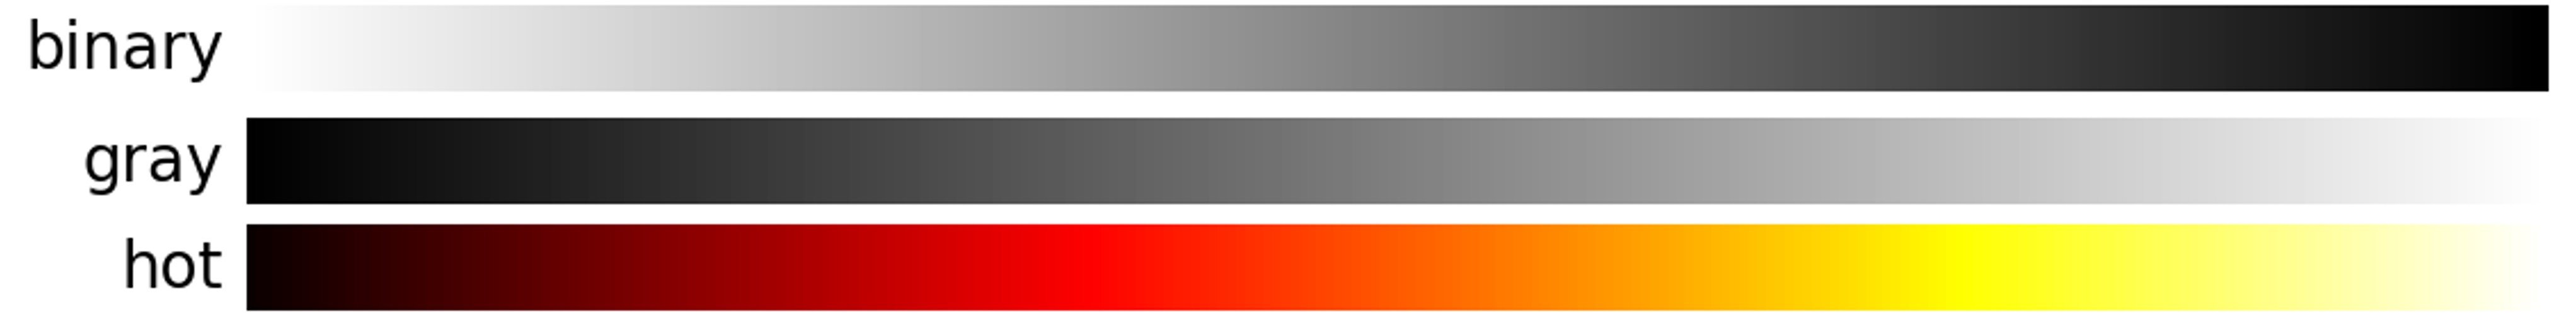
\includegraphics[width=\textwidth]{figures/chap05_colormap.jpg}
  \bicaption{三种颜色映射}{Three color maps}
  \label{fig:chap05_colormap}
\end{figure}

接下来,不同模态的影像值将采用不同的颜色映射,以增强影像中各区域之间的对比度和其可视性效果,如算法\ref{algo:chap05_colormap}所示。

\begin{algorithm}
  \caption{医学影像着色处理}
  \label{algo:chap05_colormap}
  \SetKwInOut{Input}{输入}
  \SetKwInOut{Output}{输出}
  \Input{医学影像$\mathcal{I}$}
  \Output{颜色映射$cm$}
  \vspace{5pt}

  \lIf(\tcp*[f]{无需进行着色处理}){$\mathcal{I} = \text{RGB}$}{$cm \leftarrow \text{None}$}
  \lElseIf(\tcp*[f]{gray体现不同解剖结构的层次}){$\mathcal{I} \in \{CT,MRI\}$}{$cm \leftarrow \text{gray}$}
  \uElseIf{$\mathcal{I} \in \{PET,NM\}$}{
    \lIf(\tcp*[f]{hot在融合时强调高摄取区域}){双模态融合可视化}{$cm \leftarrow \text{hot}$}
    \lElse(\tcp*[f]{单模态可视化}){$cm \leftarrow \text{binary}$}
  }
  \lElse{$cm \leftarrow \text{gray}$}
\end{algorithm}

在完成医学影像的颜色映射之后,重要的一步是考虑可视化区域的尺寸\((w,h)\)、三维医学影像在各个方向上的尺寸\((x,y,z)\)以及体素间距(Spacing\(=(s_x,s_y,s_z)\))。这一步骤是为了保证医学影像能够完整地填充整个可视化区域,以便用户能够得到一个清晰且准确的视图。因此,在进行三维医学影像切片的可视化处理时,需要计算相应的缩放比例,以便影像切片能够适配可视化区域。相关的缩放比例计算公式如下:
\begin{equation}
  \begin{aligned}
    \mathcal{S}_x^{h} & = s_y \times min(\frac{h}{z \times s_z}, \frac{w}{y \times s_y}) & \quad \mathcal{S}_x^{w} & = s_z \times min(\frac{h}{z \times s_z}, \frac{w}{y \times s_y}) \\
    \mathcal{S}_y^{h} & = s_x \times min(\frac{h}{z \times s_z}, \frac{w}{x \times s_x}) & \quad \mathcal{S}_y^{w} & = s_z \times min(\frac{h}{z \times s_z}, \frac{w}{x \times s_x}) \\
    \mathcal{S}_z^{h} & = s_x \times min(\frac{h}{x \times s_x}, \frac{w}{y \times s_y}) & \quad \mathcal{S}_z^{w} & = s_y \times min(\frac{h}{x \times s_x}, \frac{w}{y \times s_y}) \\
  \end{aligned}
  \label{eq:chap05_scale}
\end{equation}
其中,\(\mathcal{S}_\cdot^{h},\mathcal{S}_\cdot^{w}\)分别代表三维影像中,垂直于\(\cdot\)轴的切片在可视化过程中,所需应用在高度与宽度方向上的缩放比例。

最终,三维医学影像的对应切片将由可视化模块根据预设的坐标及视图参数来进行展现。当进行双模态影像的融合展示时,首先是在两种不同模态的影像之间采用第四章中介绍的方法进行配准。完成配准后,依据设定的坐标和视图参数,两种模态的影像切片将被融合展示。图像融合可以采用以下加权平均的计算公式:
\begin{equation}
  \text{Image} = \alpha \times \text{Image}_1 + \beta \times \text{Image}_2
  \label{eq:chap05_fusion}
\end{equation}
其中,\(\text{Image}_1,\text{Image}_2\)分别代表了待融合的的两幅图像,而融合系数\(\alpha, \beta\),分别取值为0.3和0.7,用以控制融合过程中各图像的权重。

对于三维展示,本章提出的方法采用了Visualization Toolkit(VTK)库来实现医学影像的三维可视化处理。首先,将医学影像数据包含的三维矩阵和体素间距以及自定义的影像原点导入到VTK中,并转换成适合VTK处理的图像格式。为了确保生成的三维影像中心位于坐标原点\((0,0,0)\),将医学影像的原点设定为:
\begin{equation}
  \begin{aligned}
    o_x & = -0.5 \times size_x \times spacing_x \\
    o_y & = -0.5 \times size_y \times spacing_y \\
    o_z & = -0.5 \times size_z \times spacing_z \\
  \end{aligned}
\end{equation}
其中,\(o_x,o_y,o_z\)分别代表医学影像在三维空间中的原点坐标,\(size_x,size_y,size_z\)分别代表医学影像在各轴方向上的大小,\(spacing_x,spacing_y,spacing_z\)则为各轴方向上的体素间距。

随后,可视化模块使用了基于光线投射的体渲染技术,该技术通过射出光线,对体数据进行采样与体素插值,从而生成包含了透明度、颜色以及光照效果的三维影像,创造出具有立体感的体渲染图,如图\ref{fig:chap05_view_3D}所示。

考虑到该体渲染技术的特性,可视化模块设定了将医学影像的影像值转换为相应颜色以及透明度的映射表,并设置了必要的光照参数,包括环境光照、漫反射光照和镜面反射光照的强度。在三维模型构建完成后,通过调整观察相机的位置和方向,可以生成完整详尽的三维视图,以供医学专家进行深入分析和解读。具体而言,为展示完整的三维医学影像,相机的视角设定为60°,焦点设置在\((0,0,0)\),朝上方向设置为\((0,0,1)\),位置定位在\((0,P_y,0)\)。其中\(P_y\)的计算公式如下:
\begin{equation}
  P_y = -0.5 \times \max(size_x \times spacing_x, size_z \times spacing_z) \div \tanh(\pi / 6)\\
\end{equation}

在双模态融合展示方面,可视化模块依据以上方法,分别对两种不同模态的医学影像进行独立的三维渲染并直接进行展示,如图\ref{fig:chap05_view_3DF}所示。

\subsection{影像分析模块}

在完成可视化模块的处理后,影像分析模块会给二维和三维展示的医学影像提供各种功能。如图\ref{fig:chap05_view_2D}和\ref{fig:chap05_view_2DF}所示,在二维影像分析时,包含了全部功能的工具栏位于标签页顶部。包含视图、坐标和对应影像值的信息区域与可视化区域内的影像切片及蓝色十字标记相互联动,任何一处发生变动,其他位置也会随之更新。主要的映射关系包括:
\begin{enumerate}
  \item \(\text{鼠标位置} \rightarrow \text{场景位置} \rightarrow \text{图像坐标}\)\label{en:chap05_1}
  \item \(\text{图像坐标} \rightarrow \text{场景位置}\)\label{en:chap05_2}
\end{enumerate}

坐标信息可以直接修改,也可以通过鼠标滑轮。鼠标左键可移动蓝色十字,视图也可以进行切换。操作按钮提供了实施旋转、镜像翻转以及图像重置的功能。普通按钮允许用户修改鼠标左键的操作,以实施影像的平移变换,而切换按钮则改变鼠标滚轮的作用,从而实现影像的缩放变换。所有这些操作均通过应用仿射变换矩阵来完成。二维仿射变换矩阵如下所示:
\begin{equation}
  \left[
    \begin{array}{ccc}
      a & b & t_x \\
      c & d & t_y \\
      0 & 0 & 1   \\
    \end{array}
    \right]
  \label{eq:chap05_affine_mat}
\end{equation}
其中,\(a\)和\(d\)表示缩放因子,\(b\)和\(c\)用于旋转变换之中,\(t_x\)和\(t_y\)表示平移量。通过调整这些参数,可以实现不同的仿射变换,如下所示:
\begin{equation}
  \begin{array}{ccc}
    \text{旋转} & \text{缩放} & \text{镜像} \\
    \left[
      \begin{array}{ccc}
        \cos(\theta) & -\sin(\theta) & 0 \\
        \sin(\theta) & \cos(\theta)  & 0 \\
        0            & 0             & 1 \\
      \end{array}
    \right]     &
    \left[
      \begin{array}{ccc}
        s_x & 0   & 0 \\
        0   & s_y & 0 \\
        0   & 0   & 1 \\
      \end{array}
    \right]     &
    \left[
      \begin{array}{ccc}
        -1 & 0 & 0 \\
        0  & 1 & 0 \\
        0  & 0 & 1 \\
      \end{array}
      \right] \quad
    \left[
      \begin{array}{ccc}
        1 & 0  & 0 \\
        0 & -1 & 0 \\
        0 & 0  & 1 \\
      \end{array}
    \right]                                 \\
  \end{array}
  \label{eq:chap05_affine}
\end{equation}
通过对比度按钮可以调节视图中医学影像的对比度,这是通过在弹出的窗口中输入窗位\(w_c\)和窗宽\(w_w\),或者最大值\(ma\)和最小值\(mi\)来实现的。具体而言,对医学影像值\(v\)的计算公式如下所示:
\begin{equation}
  \begin{aligned}
    ma & = w_c + 0.5 \times w_w                       \\
    mi & = w_c - 0.5 \times w_w                       \\
    v  & = \frac{\min(\max(mi, v), ma) - mi}{ma - mi} \\
  \end{aligned}
  \label{eq:chap05_constrast}
\end{equation}

标签按钮可用来导入NIfTI格式的标签数据,以渲染分割图或显示边界框;标签滑块则可调整标签图的透明度。

在三维影像分析时,所有功能均汇聚于标签页顶部的工具栏中,如图\ref{fig:chap05_view_3D}和\ref{fig:chap05_view_3DF}所示。视图按钮允许用户选择性地渲染特定的影像数据,以此进行独立的视图展示。标签按钮用于导入NIfTI或Json格式的标签数据,这使得用户能够渲染出三维的立体边界框和关联分类标签。通过标签滑块,用户可细致地调整标签图层的透明度,以便更好地视察底层的医学影像。人体按钮采用了第四章中介绍的人体保留算法,专门针对PET/CT影像数据进行优化处理,去除掉机床等无关区域。此外,鼠标左键的操作,实现了观察摄像头在以原点为中心的虚拟球面的移动,来达成三维医学影像的旋转变换。同时,通过鼠标滑轮调节,可以改变三维影像与观察摄像头之间的距离,从而实现三维影像的缩放效果。

\section{案例分析}

在本节中,将示范自动诊断与可视化方法对上海市第六人民医院核医学科2016年的三个病例的应用实践:

(1)患者A在膝关节置换手术后两月接受了膝部的动态骨显像扫描,医生通过影像分析初步判定膝假体处可能感染,并在评估病症、临床表现以及影像与血液检验结果后,确诊为膝关节假体感染;

(2)患者B在髋关节置换术后两年进行了髋部动态骨显像扫描。经影像学分析后,医生怀疑髋假体发生感染,最终依据全面诊断确诊为假体髋关节感染;

(3)患者C在右股骨骨折治疗后接受PET/CT扫描。经过影像学判断,疑似存在感染性病灶。借助微生物培养、病理分析及临床综合判断,确认患有骨折相关感染。

\begin{figure}[htbp]
  \centering
  \bisubcaptionbox{打开文件\label{fig:chap05_example01_open}}{Opening a file}[0.49\textwidth]{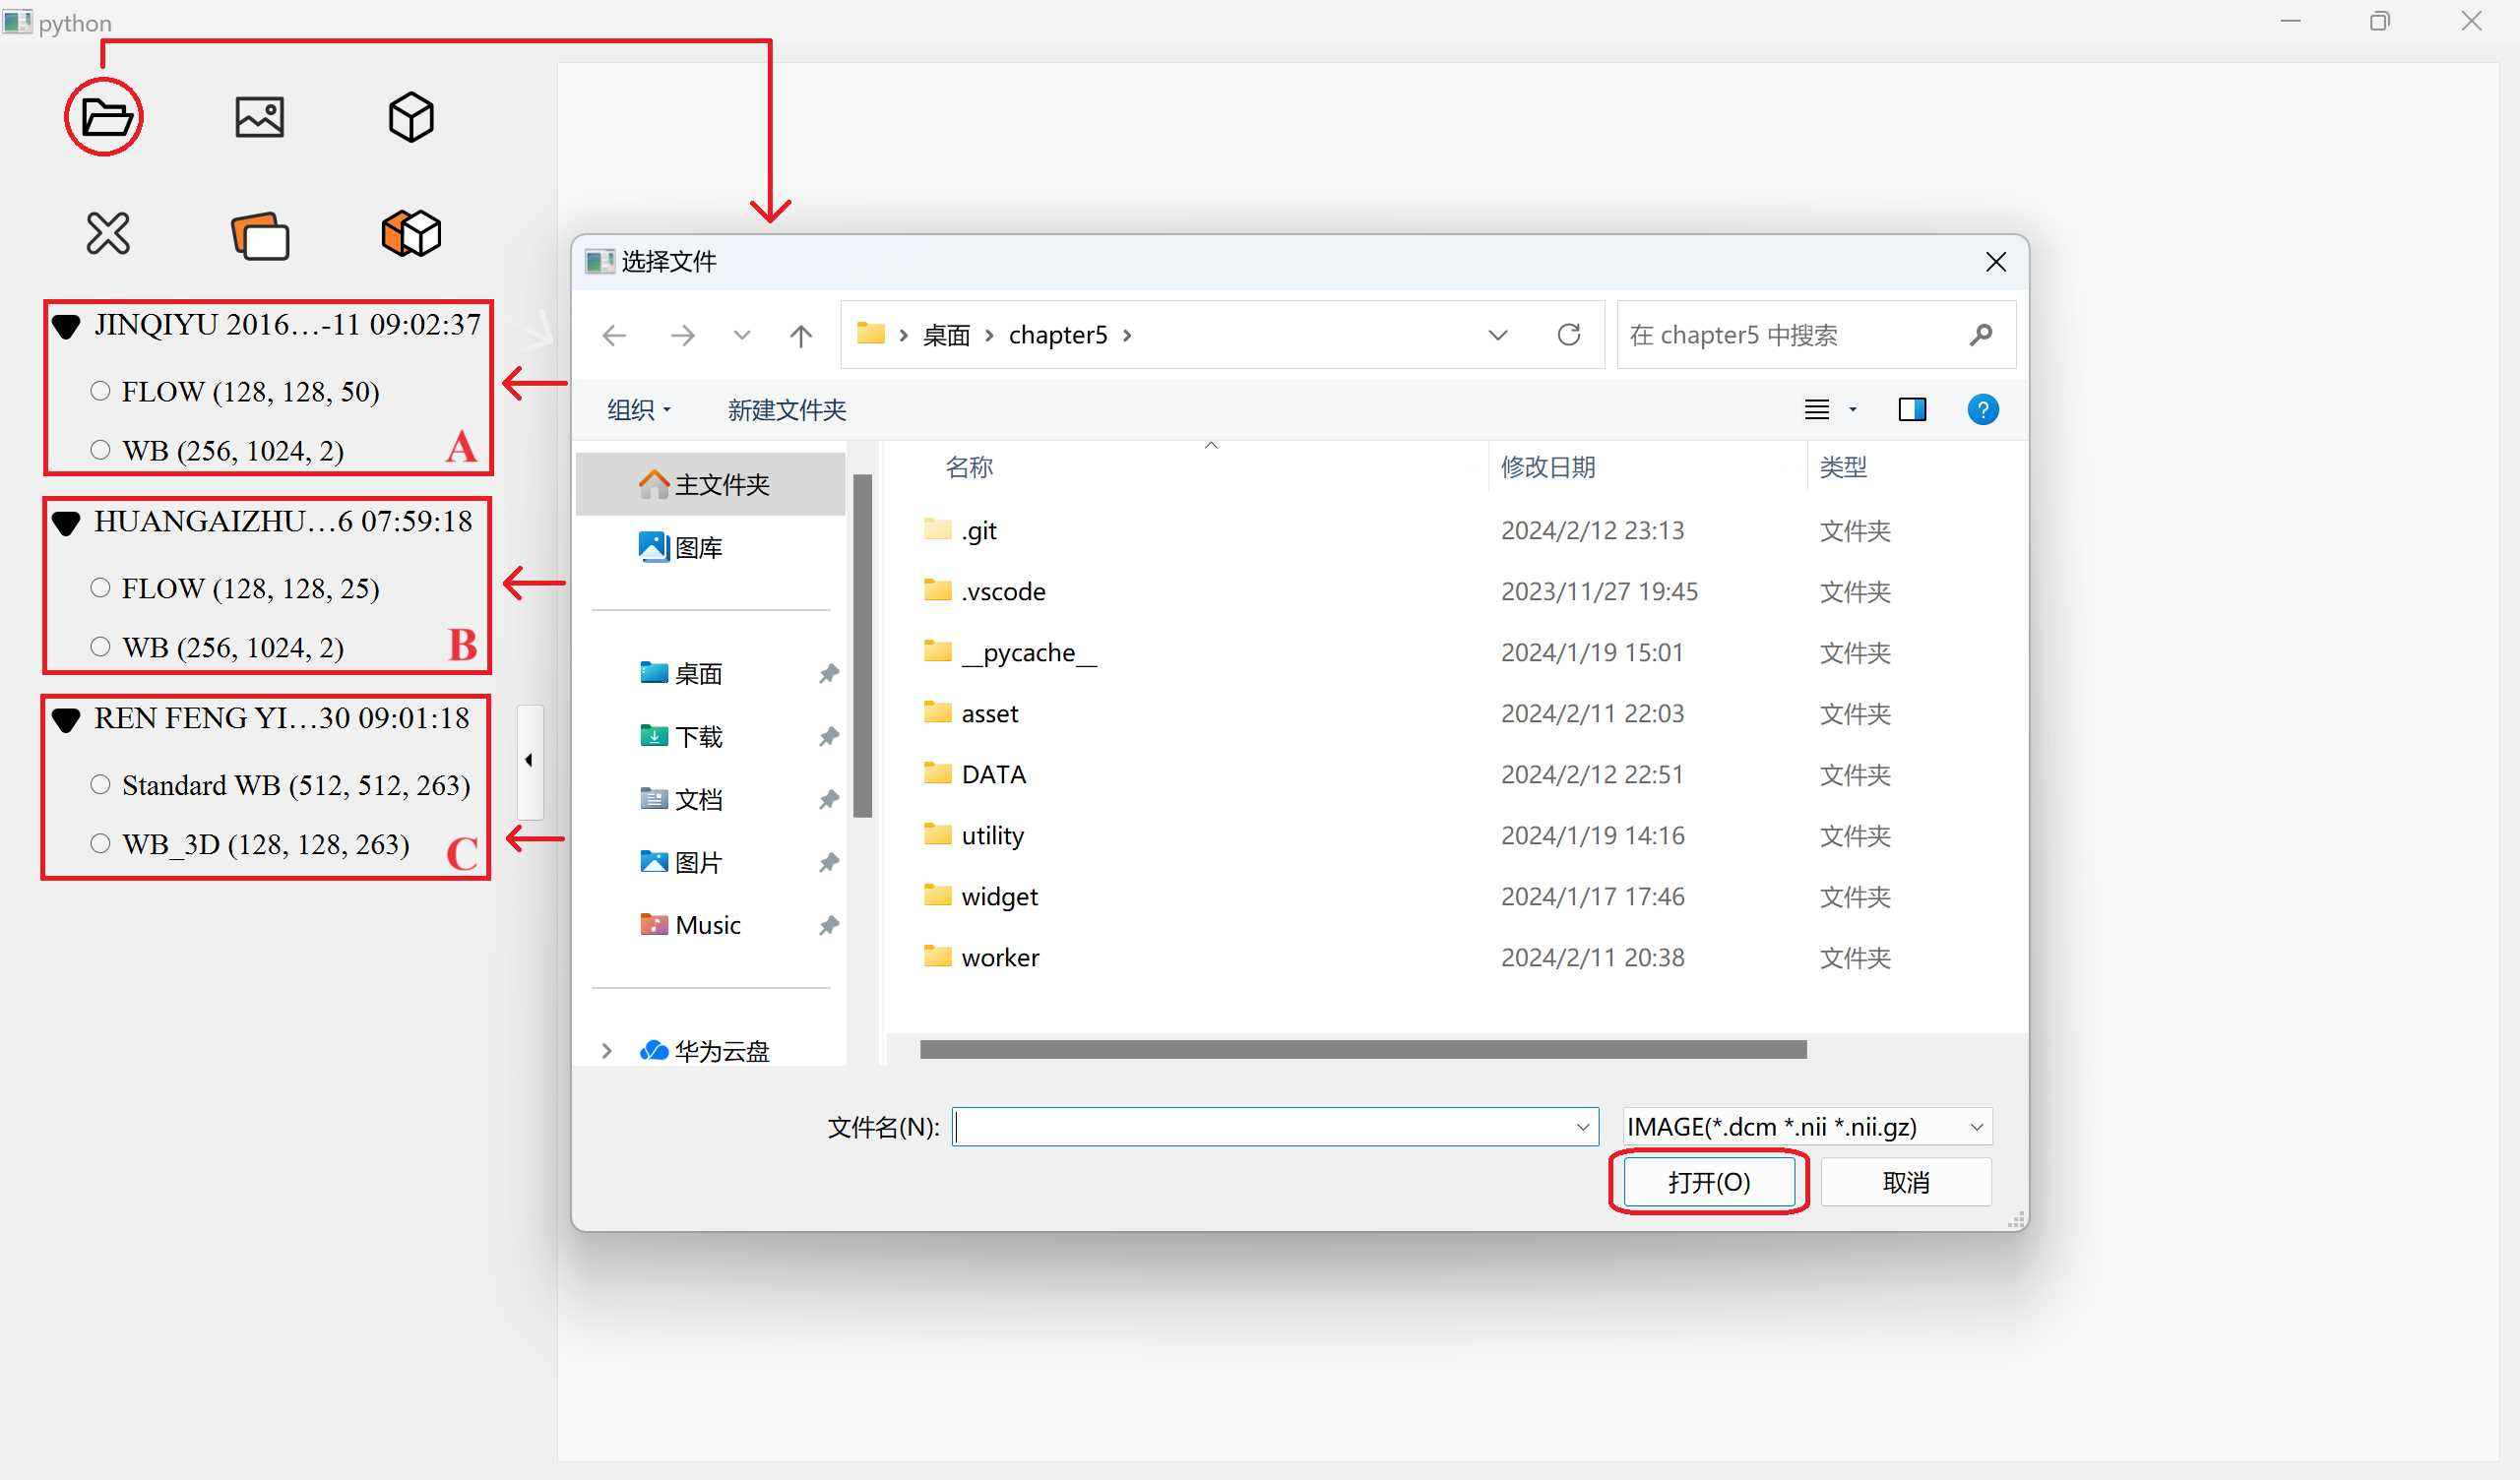
\includegraphics[width=0.49\textwidth]{figures/chap05_example01_open.jpg}}
  \bisubcaptionbox{膝部动态骨显像\label{fig:chap05_example02_vis}}{knee dynamic bone scintigraphy}[0.49\textwidth]{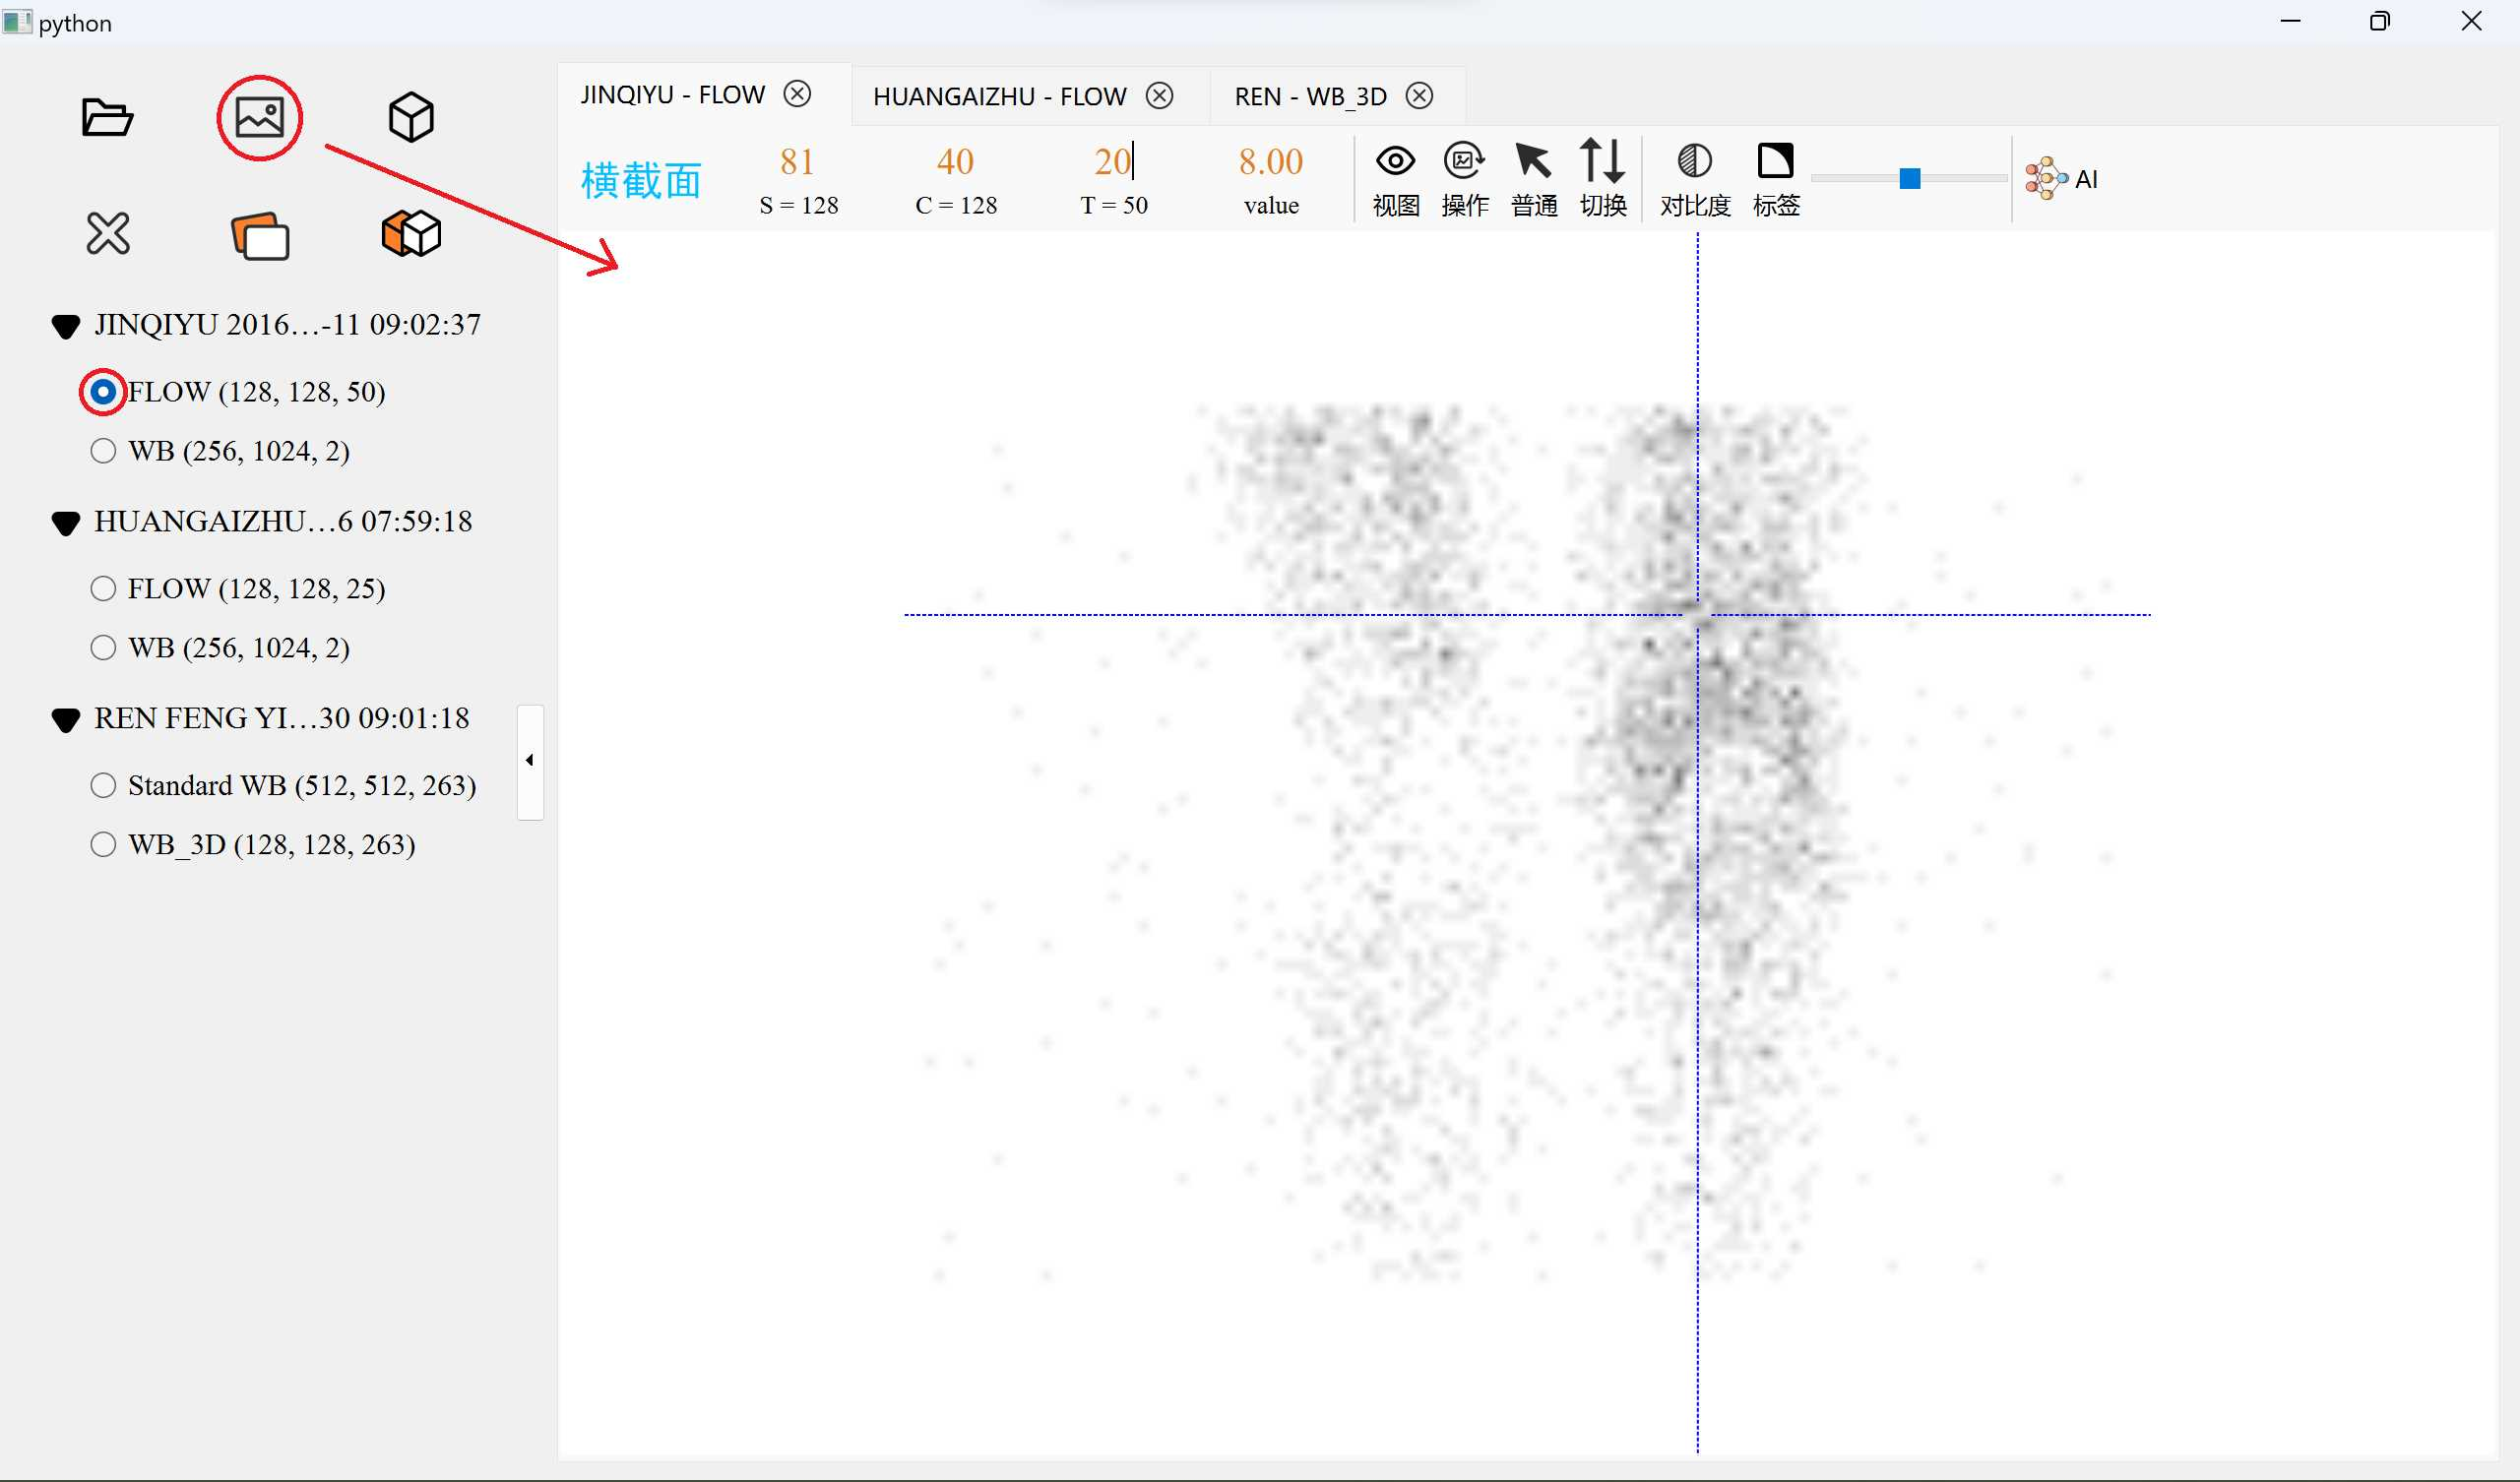
\includegraphics[width=0.49\textwidth]{figures/chap05_example02_vis.jpg}}
  \bisubcaptionbox{髋部动态骨显像\label{fig:chap05_example03_vis}}{hip dynamic bone scintigraphy}[0.49\textwidth]{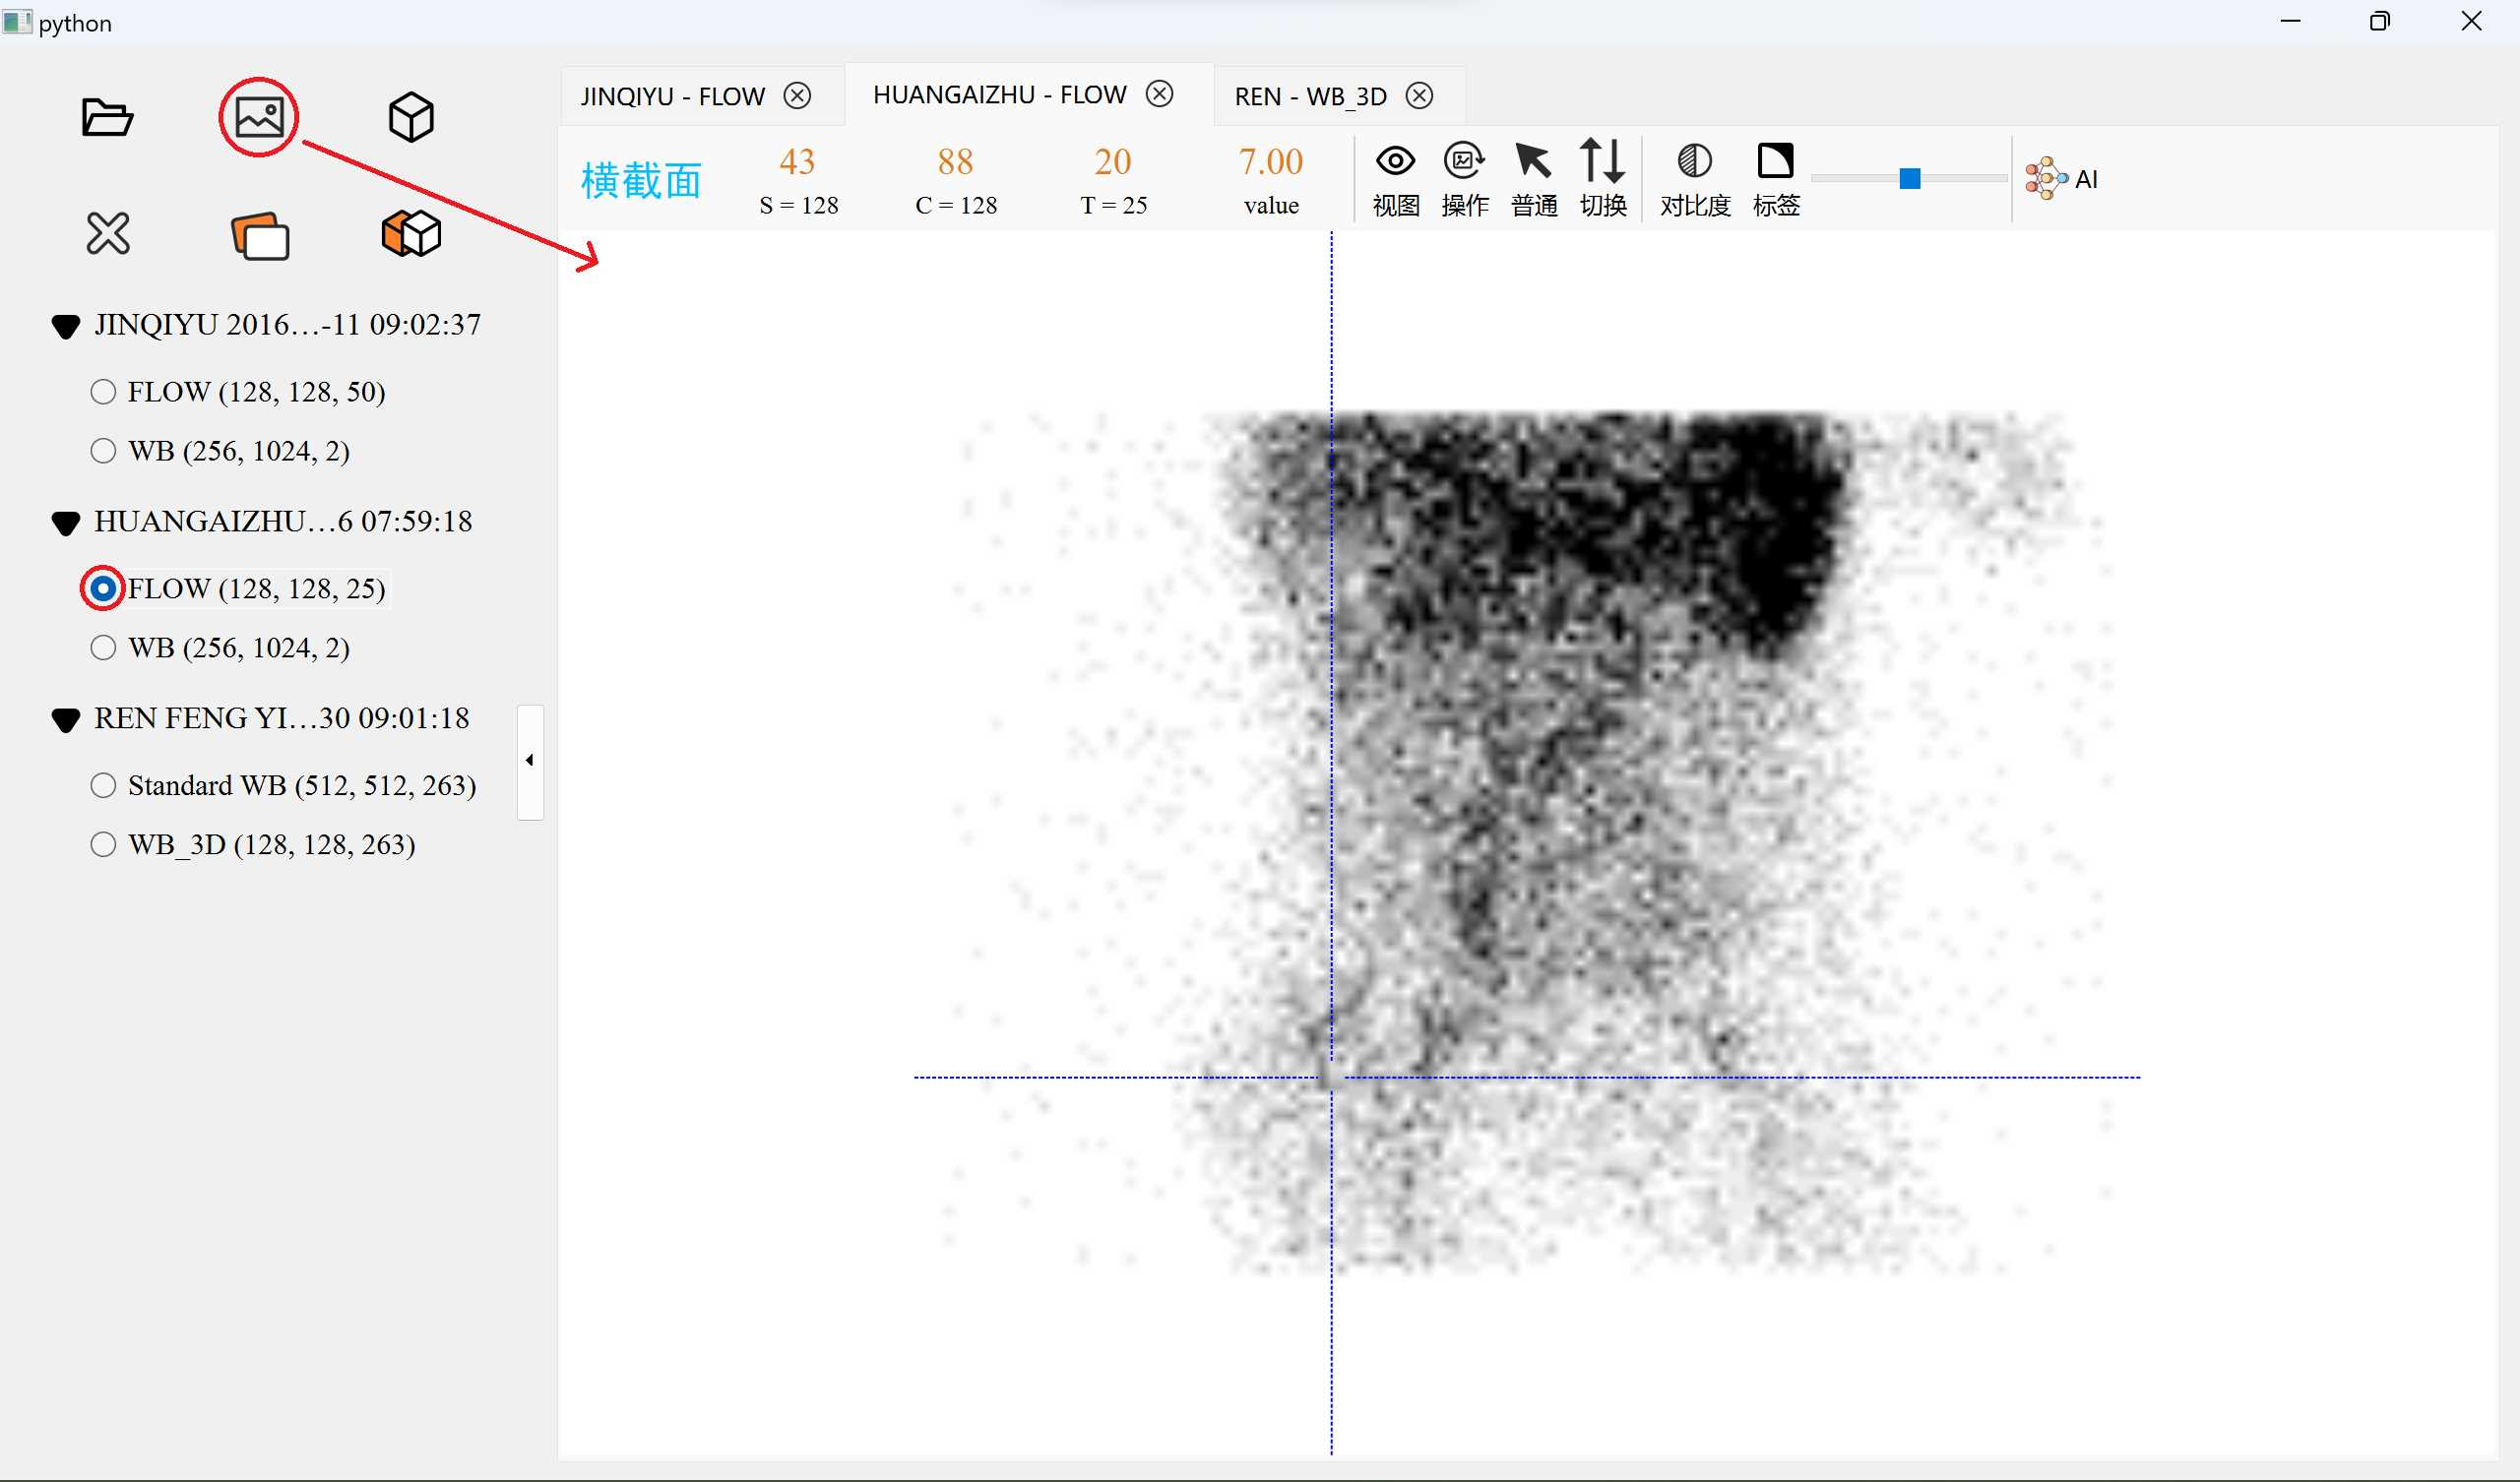
\includegraphics[width=0.49\textwidth]{figures/chap05_example03_vis.jpg}}
  \bisubcaptionbox{下肢PET/CT融合\label{fig:chap05_example04_vis}}{lower extremities PET/CT fusion}[0.49\textwidth]{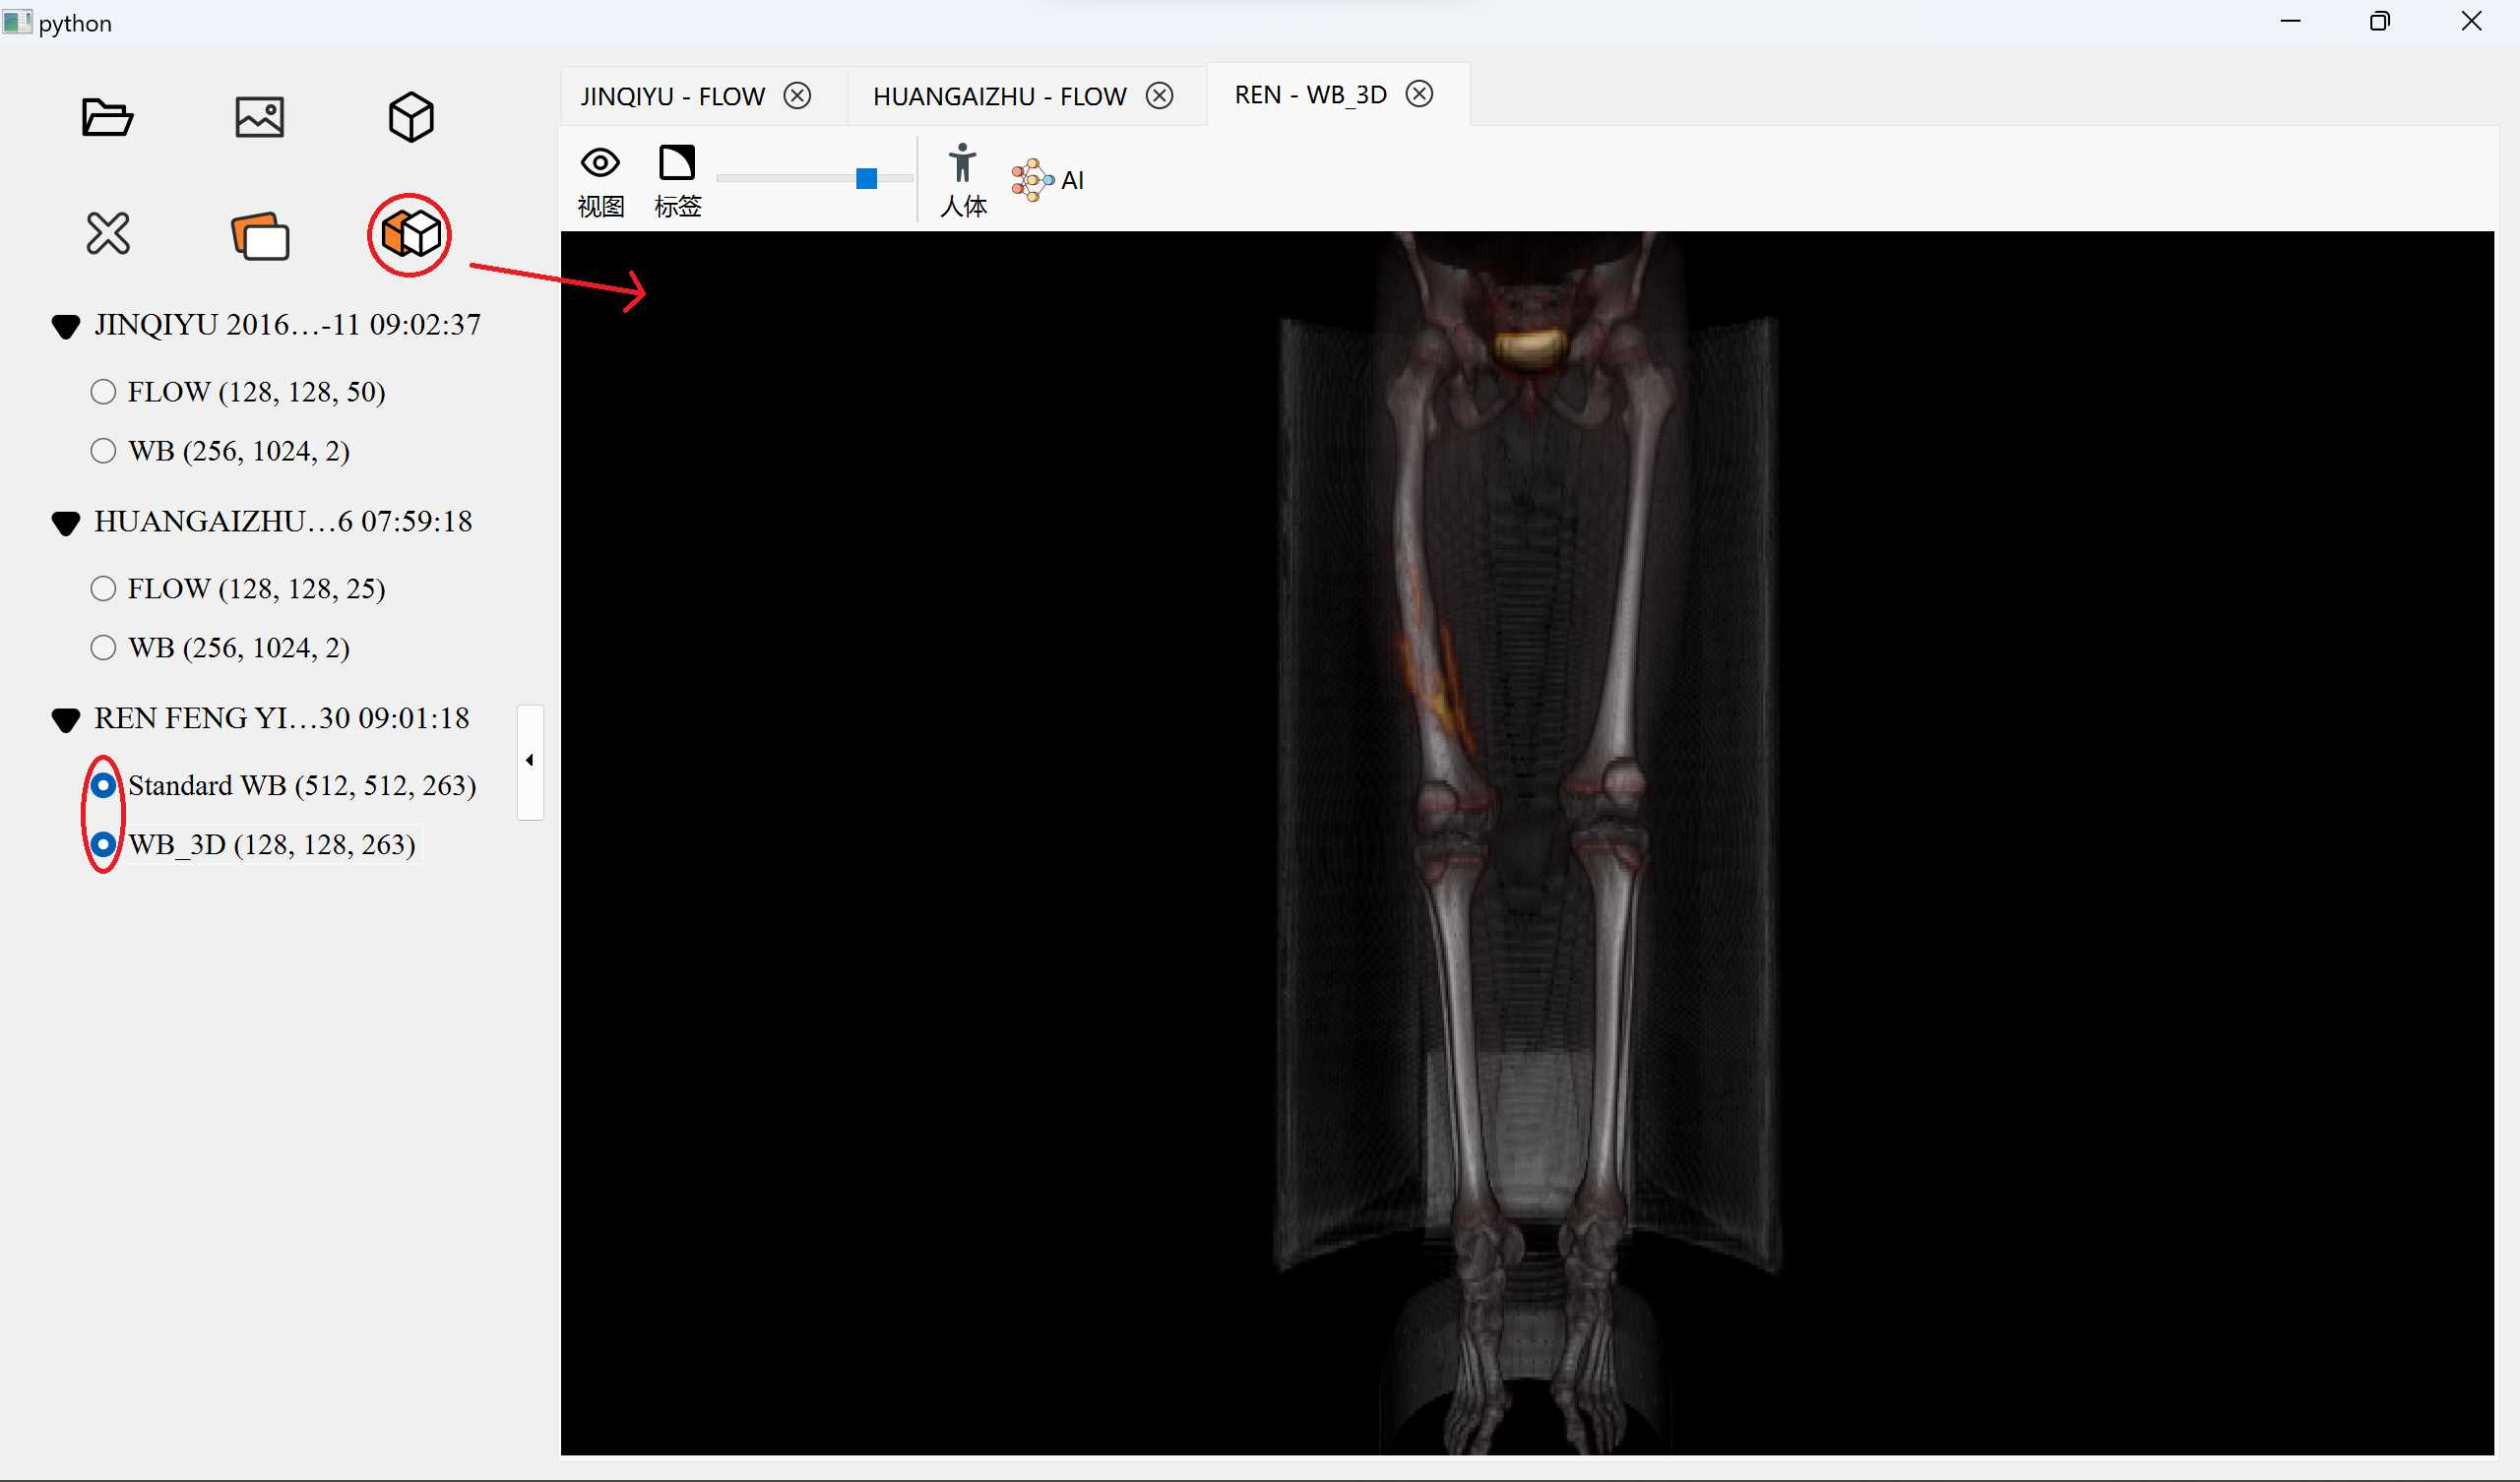
\includegraphics[width=0.49\textwidth]{figures/chap05_example04_vis.jpg}}
  \bicaption{案例可视化}{Case visualization}\label{fig:chap05_example_vis}
\end{figure}

如图\ref{fig:chap05_example01_open}所示,通过在侧边导航栏顶部的“打开文件”功能按钮,可以在启动的文件选择窗口中依次打开患者A、患者B和患者C的DICOM医学影像文件。影像文件被打开并成功解析后,结果在侧边导航栏中清晰地展示了出来。

如图\ref{fig:chap05_example02_vis}所示,通过选中患者A的动态骨显像并点击“二维影像展示”按钮,从而呈现了患者A膝部的二维可视化影像。图\ref{fig:chap05_example03_vis}则展现了类似操作过程,勾选患者B的动态骨显像并点击相同的功能按钮,实现了髋部影像的二维可视化。随后,使用可视化区域顶部的影像分析工具。通过调整影像的对比度,以获得更清晰细致的可视化效果。在此基础上,灵活地切换不同的切片,搜索并定位到最合适的影像切片。最后,移动蓝色十字光标至特定区域,以查看相应的影像值,为进一步的分析和评估提供关键信息。

通过可视化区域顶部工具栏最右侧的AI功能按钮,可以激活辅助诊断模块的自动诊断功能,并获得基于深度学习方法生成的辅助诊断建议。图\ref{fig:chap05_example_result1}所展示的是患者A的案例,辅助诊断结果建议患者存在假体关节感染的情况。同时,图\ref{fig:chap05_example_result2}中以透明红色矩形标识了患者B髋部中的感兴趣区域,并表明了患者B存在假体关节感染的诊断建议。

图\ref{fig:chap05_example04_vis}展现了患者C的PET和CT影像数据,通过选中并点击“三维影像融合”按钮后,得到的下肢立体融合影像的可视化图。此后,利用影像分析工具可以对该立体影像进行缩放和旋转操作,以便对特定感兴趣的区域进行详细的观察和分析。点击AI辅助诊断按钮后,如图\ref{fig:chap05_example_result3}所呈现的,患者C被智能辅助诊断为存在一个感染区域,并且该区域在患者C的右股骨处被一个青色立体框所标记。最后借助于视图按钮,还能够从不同角度观察并分析感染区域的影像数据,如图\ref{fig:chap05_example_result4}所示。

\begin{figure}[htbp]
  \centering
  \bisubcaptionbox{膝部\label{fig:chap05_example_result1}}{Knee}[0.49\textwidth]{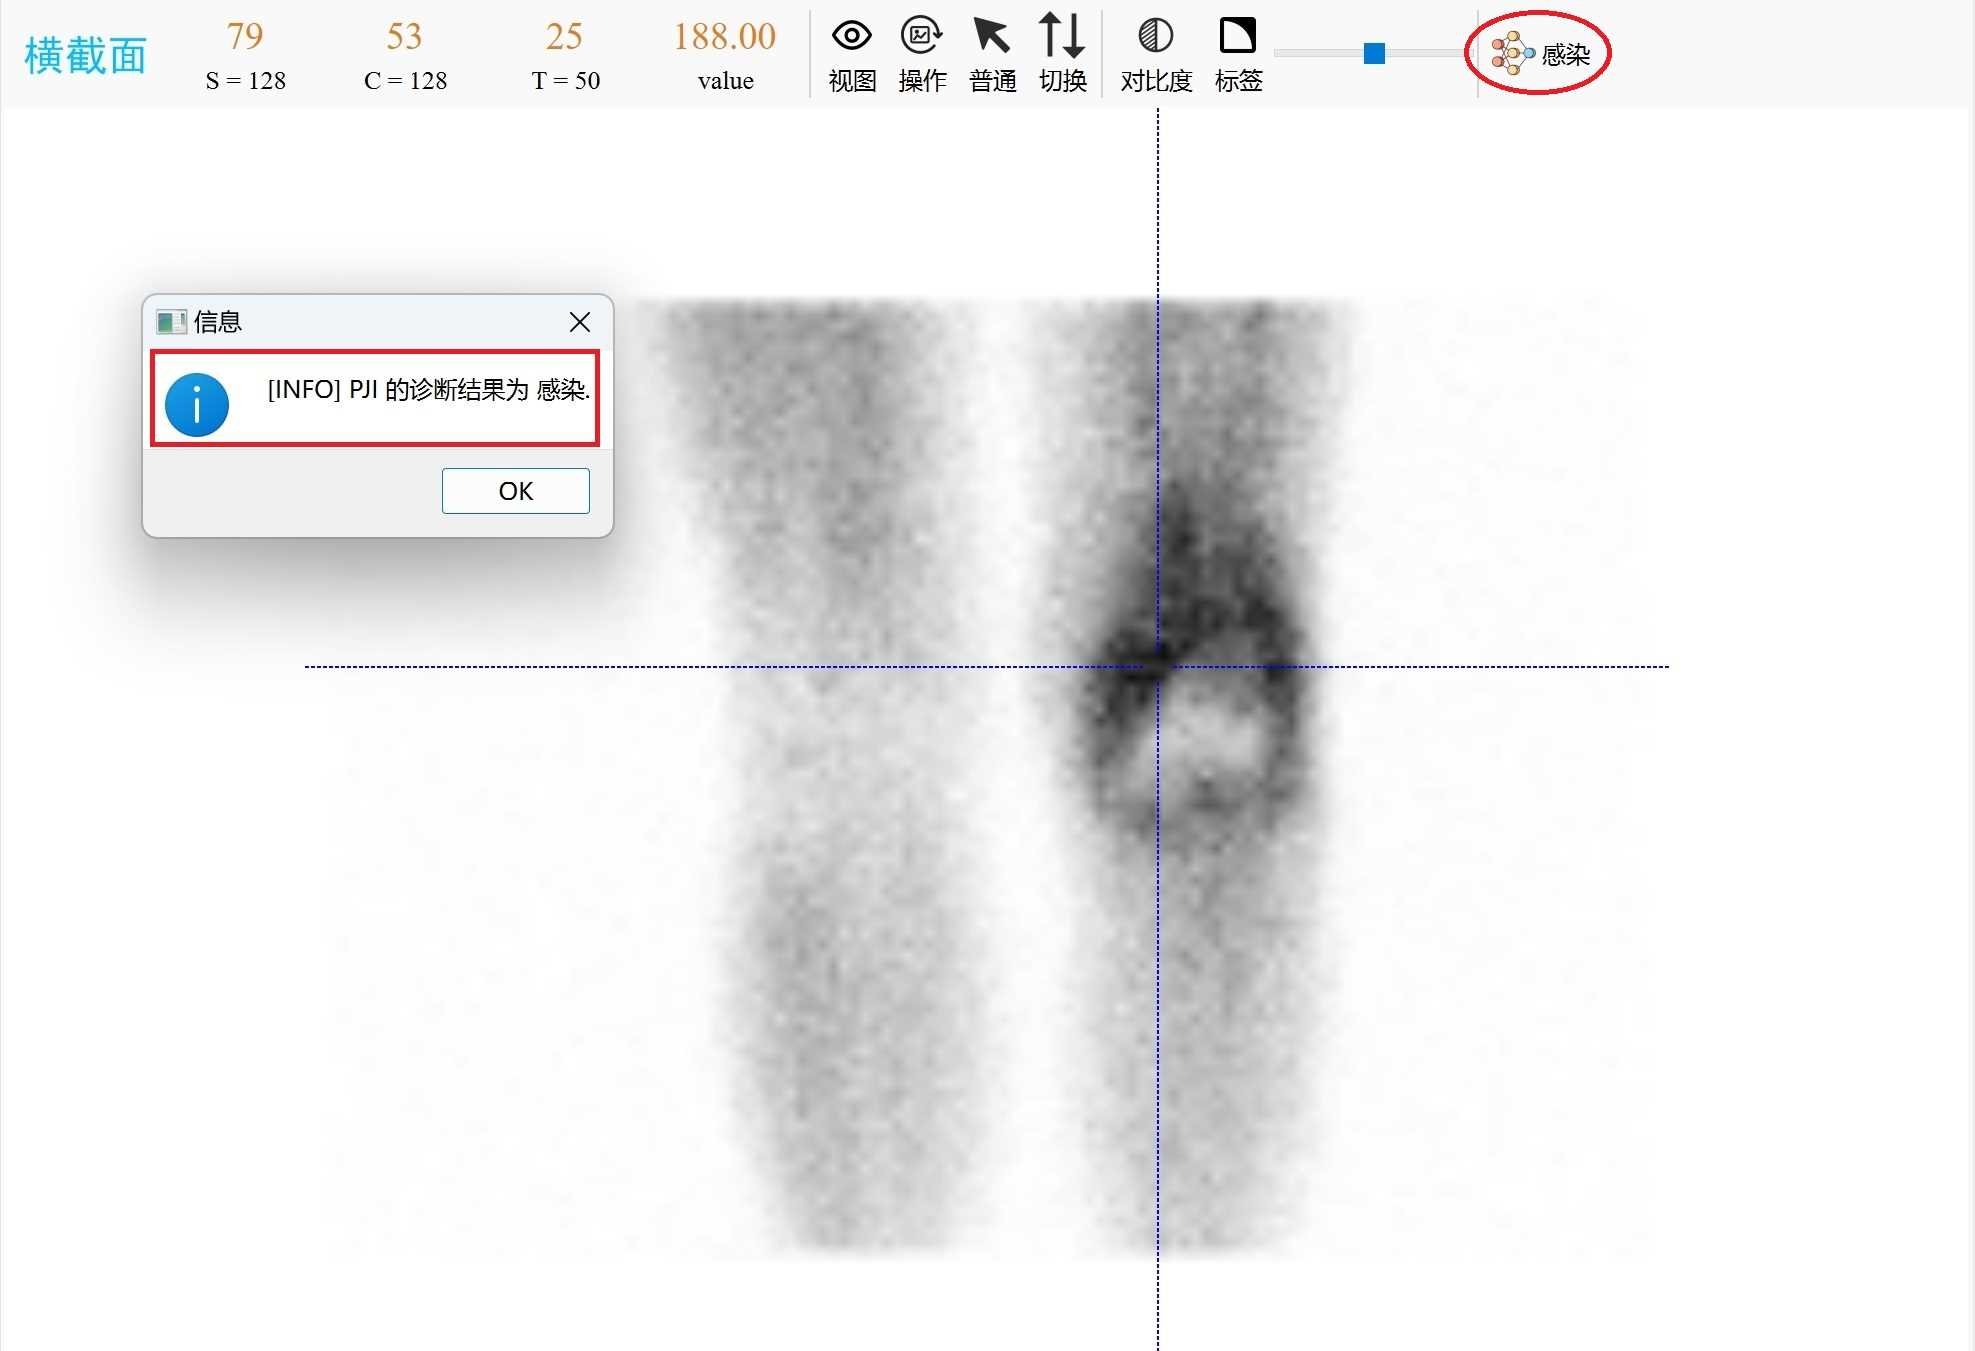
\includegraphics[width=0.49\textwidth]{figures/chap05_example_result1.jpg}}
  \bisubcaptionbox{髋部\label{fig:chap05_example_result2}}{Hip}[0.49\textwidth]{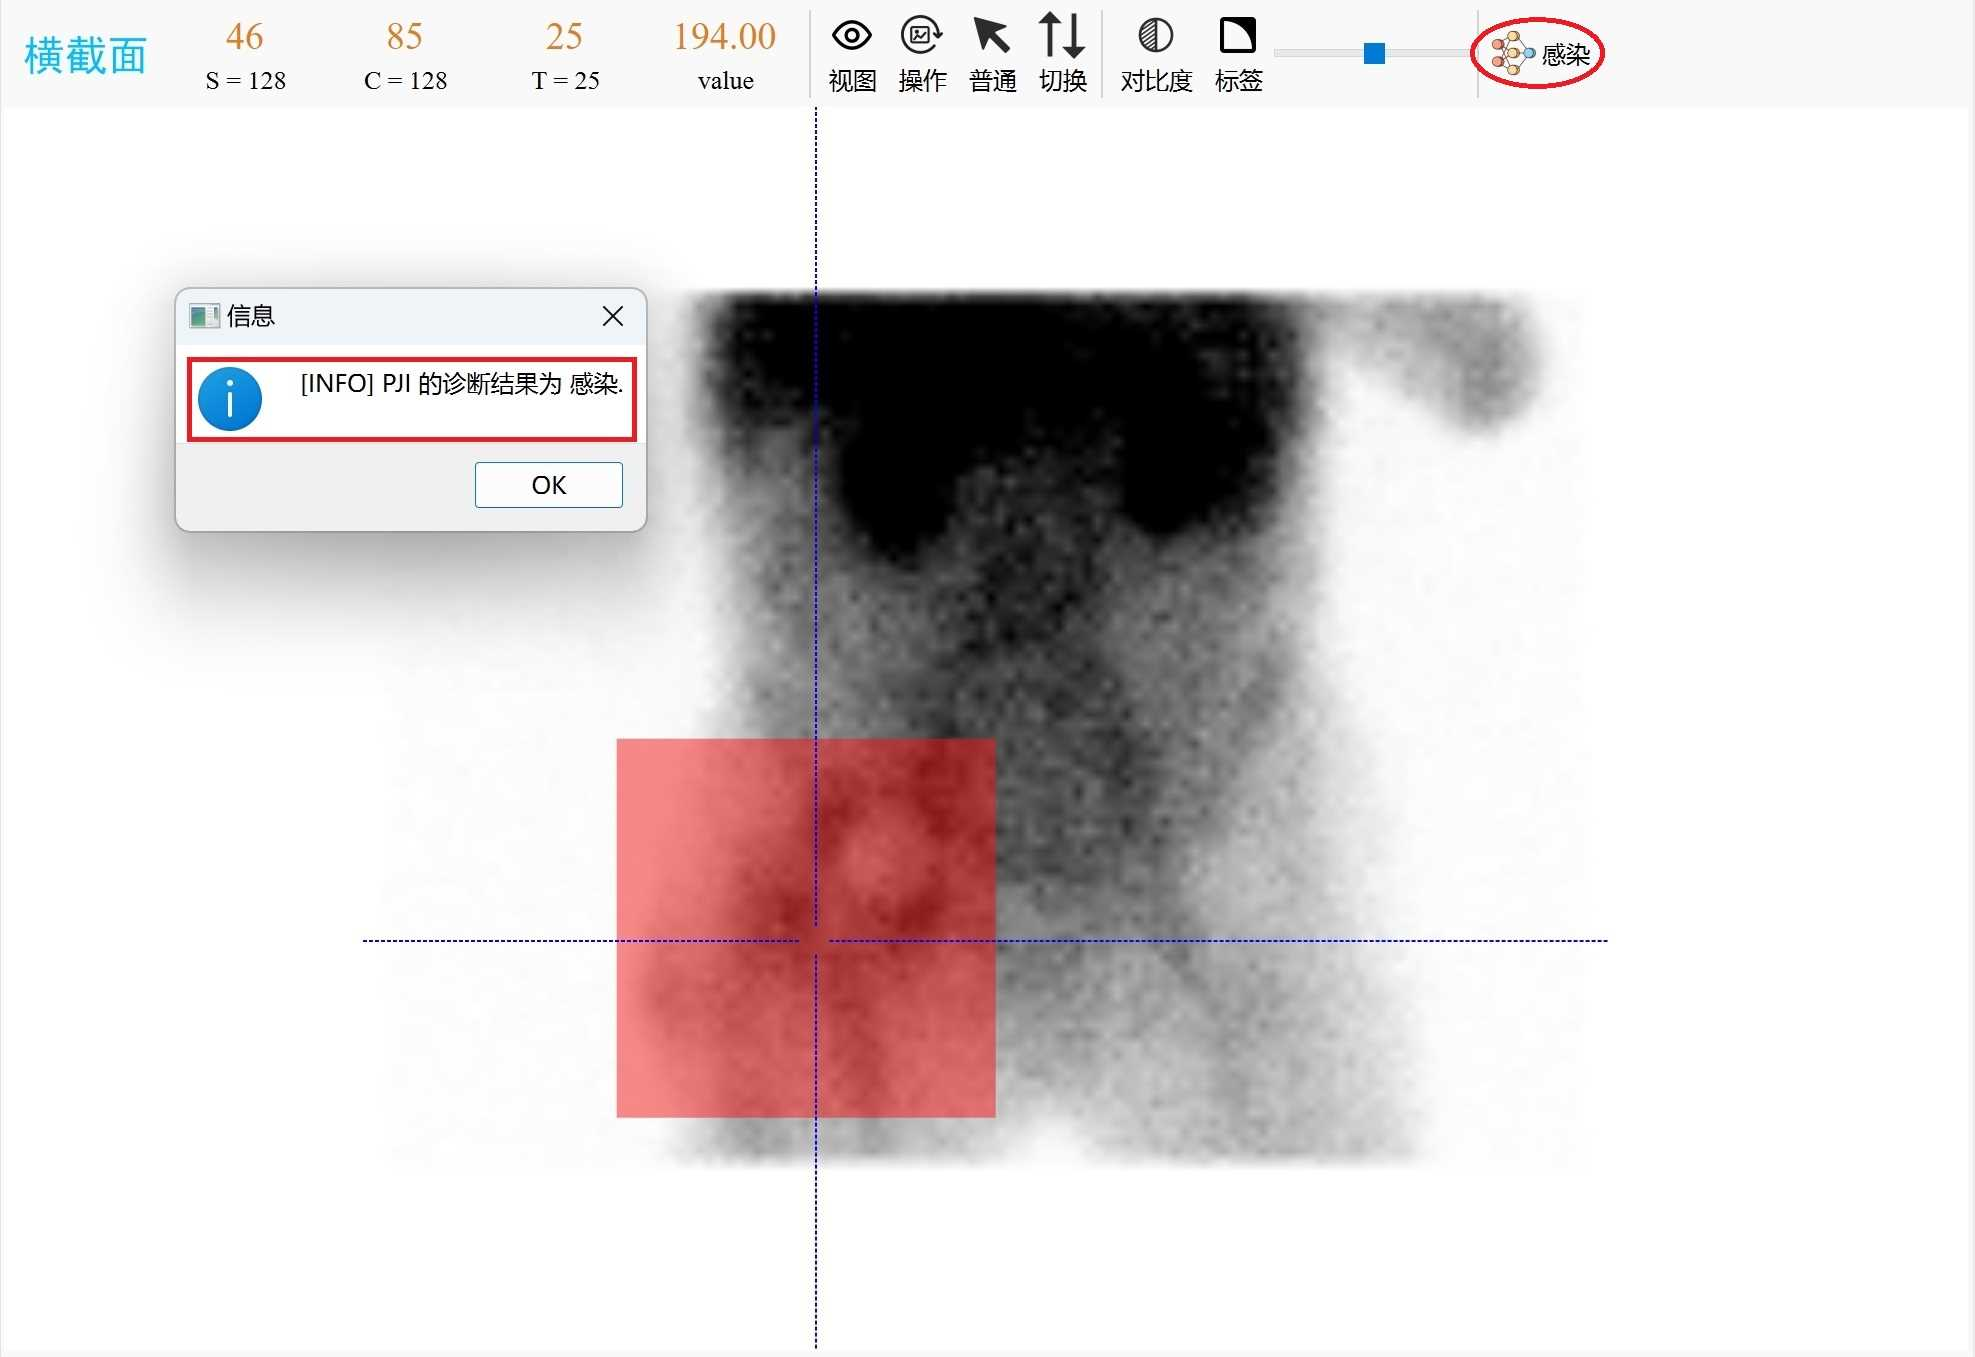
\includegraphics[width=0.49\textwidth]{figures/chap05_example_result2.jpg}}
  \bisubcaptionbox{下肢\label{fig:chap05_example_result3}}{the Lower extremities}[0.49\textwidth]{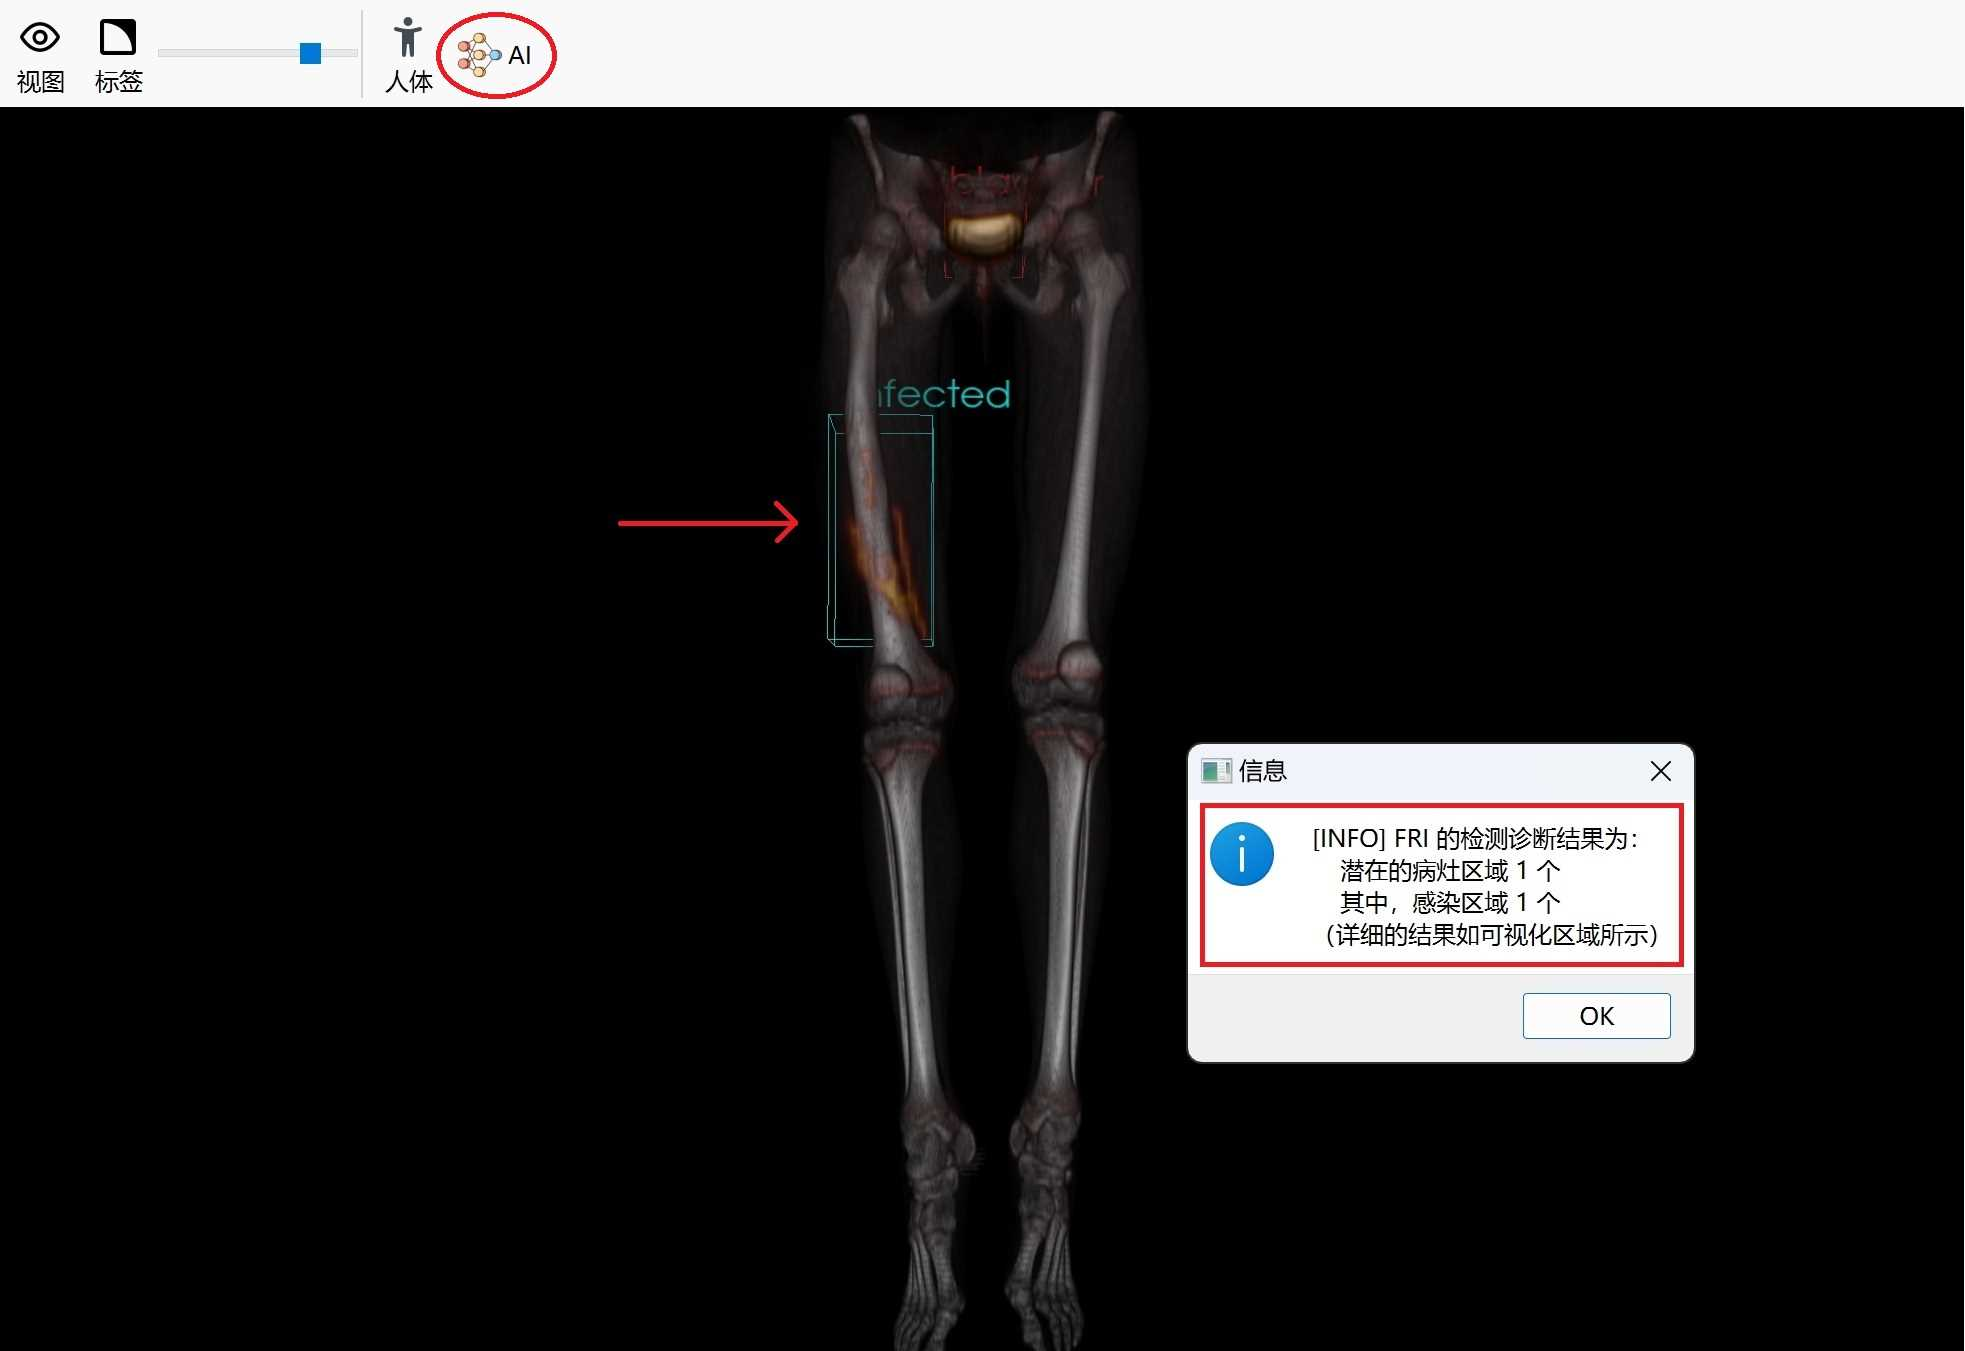
\includegraphics[width=0.49\textwidth]{figures/chap05_example_result3.jpg}}
  \bisubcaptionbox{感染病灶\label{fig:chap05_example_result4}}{infected lesion}[0.49\textwidth]{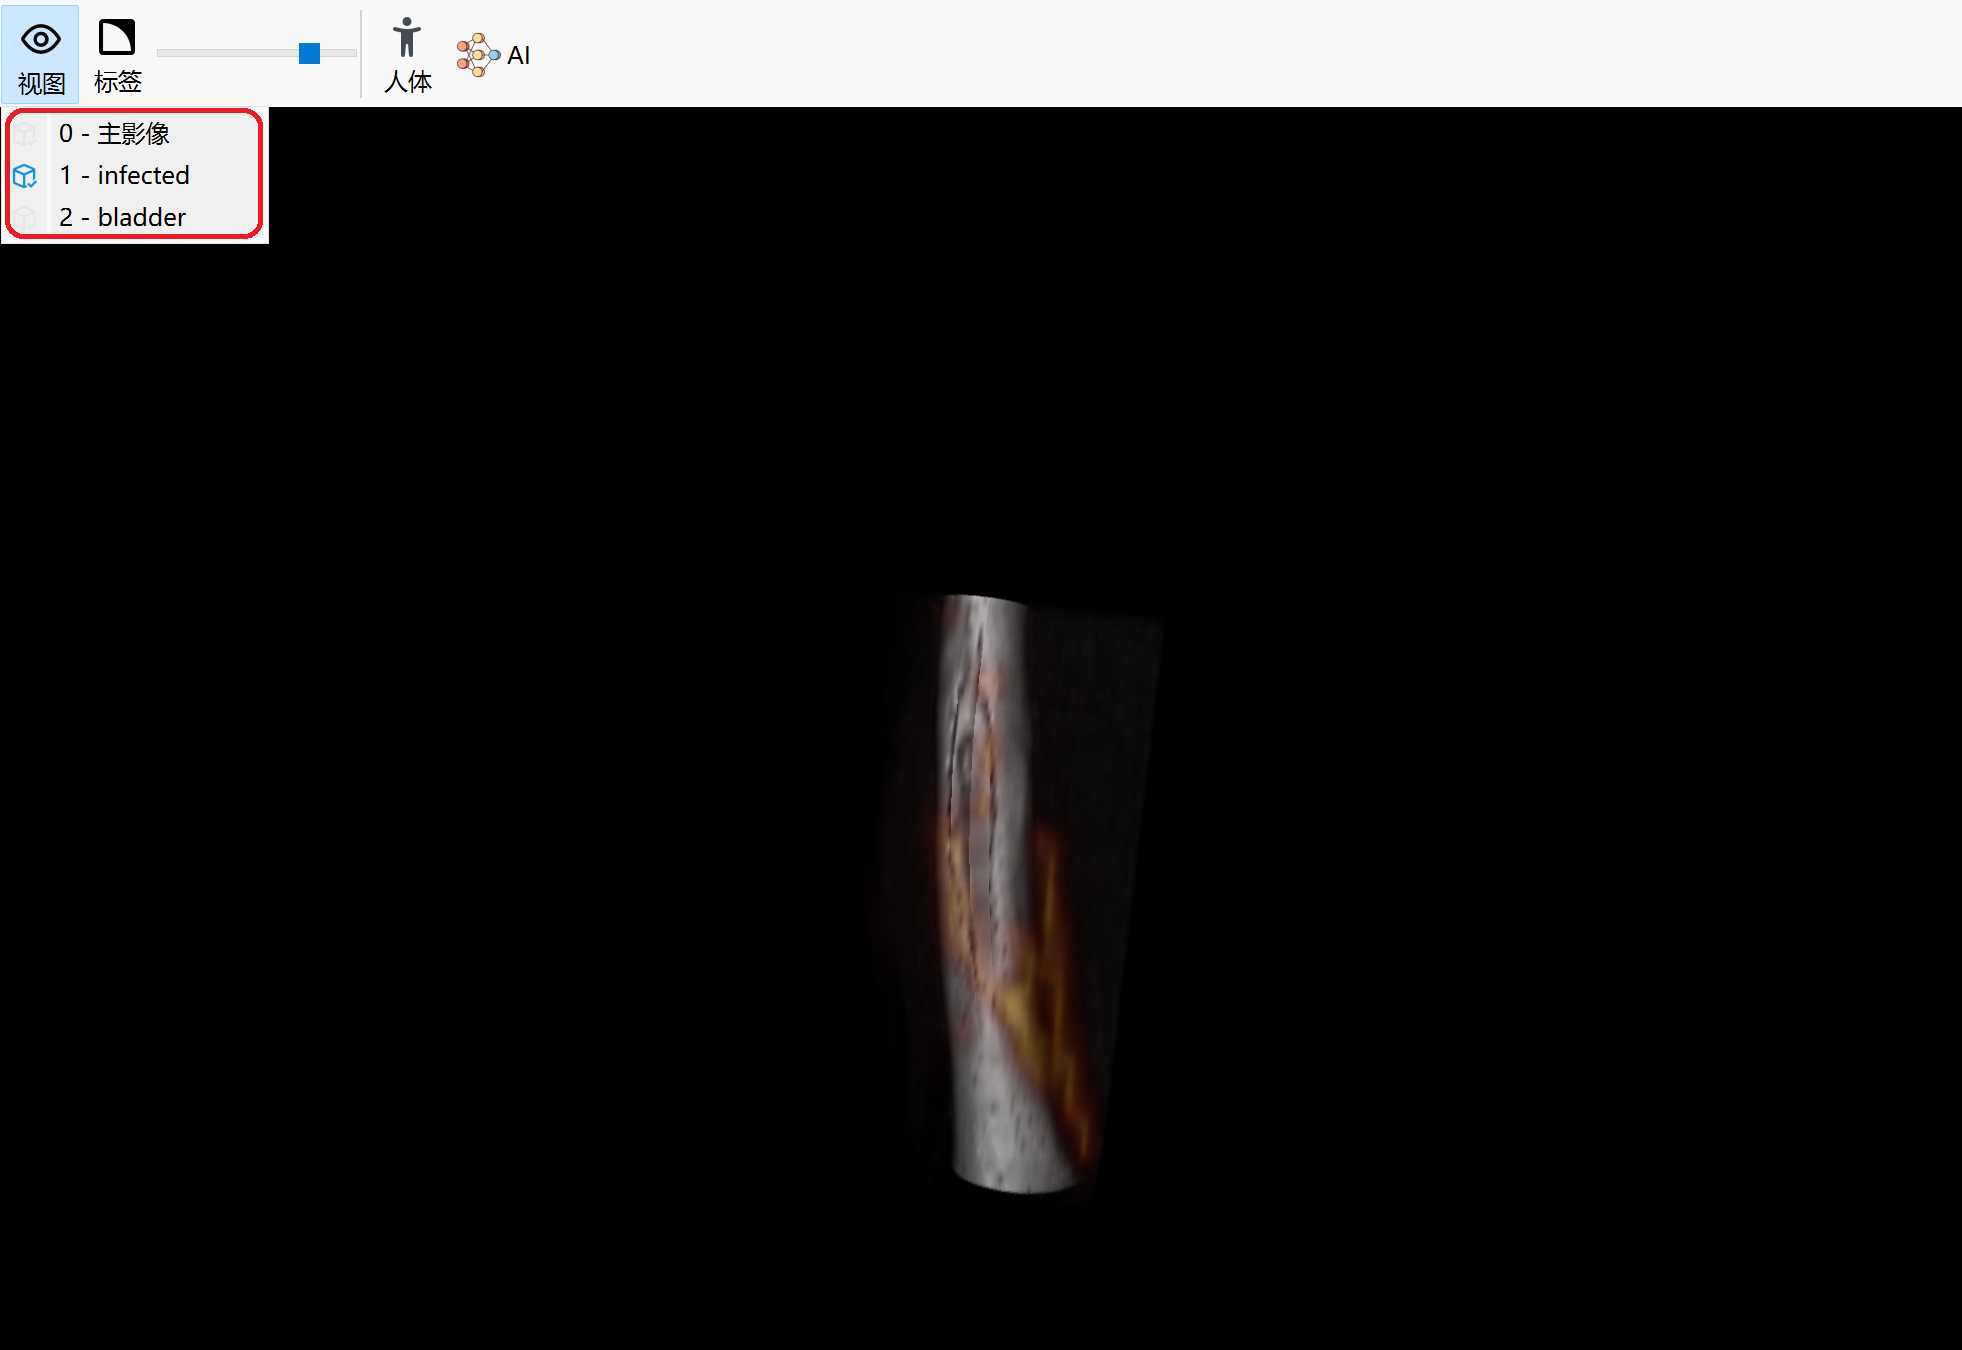
\includegraphics[width=0.49\textwidth]{figures/chap05_example_result4.jpg}}
  \bicaption{自动诊断方法}{Automatic diagnosis method}\label{fig:chap05_example_diagnose}
\end{figure}

通过对三个具体病例的详细展示和分析,提供的辅助诊断建议与经验丰富的医生所作出的诊断高度一致。这表明本章所介绍的自动诊断与可视化方法,不仅赋予了医生一个实用的影像分析工具,还可以通过整合先进的深度学习技术提出极具参考价值的辅助诊断建议。

\section{本章小结}

本章提出了一种用于骨科相关感染的自动诊断和可视化方法。此方法结合了前两章提出的假体关节感染辅助诊断框架与骨折相关感染检测与诊断框架,以便进行对动态骨扫描和PET/CT影像的自动化处理和分析。同时,本方法还包含了从文件读取解析到医学影像的各种可视化,以及涵盖多项分析工具的影像分析,实现对医学影像中潜在病灶的定位与分析。本章最后通过三个真实病例的分析,验证了提出的辅助诊断建议与患者真实情况之间基本一致。这证明了本章方法,不仅为用户提供了一个全面而高效的可视化交互和分析工具,而且有助于促进医生的临床决策和提高准确性。
% !Mode:: "TeX:UTF-8"
\chapter{总结与展望}

\section{总结}

本文聚焦于在核医学影像中进行骨科相关感染疾病的辅助诊断,具体涉及假体关节感染和骨折相关感染。动态骨显像具有时间序列特性且包含三种不同阶段的相,PET和CT可以提供更全面的三维影像信息,以及动态骨显像和PET/CT中均存在自然高摄取区域的干扰等等。针对这些问题和特点,本文提出了基于动态骨显像的假体关节感染辅助分类诊断框架和基于下肢PET/CT影像中骨折相关感染的检测与诊断框架。本文的主要工作总结如下:

(1)面对骨科相关感染领域医学影像数据集的不足,本文作者与上海市第六人民医院核医学科进行了合作,共同构建了两个核心数据集。动态骨显像数据集涵盖了2016年1月至2021年6月期间455位患者的影像及其匹配的诊断报告。PET/CT数据集则收集了2016年11月至2021年12月期间281位患者的医学影像和诊断报告。在医学专家的指导下,对这两个数据集进行了精确的数据标注,确保其高度的准确性和可信度。此外,本文还特别为动态骨显像和PET/CT影像设计了专门的数据预处理方法,旨在统一数据格式,提升影像质量,并减少无关区域和自然高摄取区域带来的不利影响。

(2)为提升动态骨显像在假体关节感染诊断中的应用效果,本文提出了一个包含了预处理和融合三维卷积与ConvLSTM的辅助诊断模型(DBS-eNet)的辅助诊断框架。DBS-eNet充分挖掘了动态骨显像多个相及其内部的图像序列信息。通过三维卷积技术,模型能够在时间维度上有效提取每幅图像的生理摄取形态特征,而ConvLSTM则在强化图像的形态特征的同时,能够捕捉图像序列中生理代谢活动的动态变化。通过实验验证,DBS-eNet在处理假体膝关节感染与假体髋关节感染诊断任务时表现出色,准确率在五折交叉验证测试中分别达到了86.48\%和86.33\%,并在与核医学专家的独立验证比较中,膝关节诊断准确率提高了13.55\%,髋关节诊断准确率与专家持平。

(3)面向下肢骨折相关感染的PET/CT影像诊断任务,本文提出了一个创新的两阶段框架——3DFRINet。该框架包含了病灶检测网络与病灶诊断分类网络。病灶检测网络通过双分支网络的架构设计和注意力机制,高效融合不同模态下的多尺度特征,实现病灶的精确定位。紧随其后的病灶诊断分类网络,运用最大强度投影技术将三维影像信息投影至二维,不仅保留了关键特征,也深入分析了感染病灶的代谢形态,以达到精准分类的目标。实验结果显示,3DFRINet在下肢PET/CT影像病灶检测任务中表现卓越,超越了其他YOLO模型,其AP\(_{25}\)指标高达0.9234;而在对骨折相关感染病灶进行诊断分类时,相比于资历较浅的核医学医师,准确率提高了11.27\%,与资深核医学医师相比也提升了4.23\%。

(4)本文最后设计了一套针对骨科相关感染的自动诊断与可视化方法。该方法融合了(2)和(3)的模型,不仅支持假体关节感染的诊断分类工作,还能自动检测并分类骨折相关感染的病灶。此外,为了适应各种医学影像模态,该方法支持二维、三维以及PET/CT融合影像的可视化分析。在功能性设计上,该方法为二维影像提供了诸如医学影像值及其坐标呈现、视图切换等功能;而在三维影像方面,则允许用户进行旋转、缩放等操作,以促进对复杂医学影像数据的理解和分析。

综上所述,本文实现了假体关节感染和骨折相关感染的完整诊断流程。实验对比、可视化方法以及案例分析都证实了本文研究的可信度。本文可以为医疗诊断提供了客观的建议,助力医学影像智能诊断领域向规范化及标准化迈进。

\section{展望}

本文成果虽已取得一定的成就,但在未来的研究中仍存在以下几个发展方向:

(1)尽管本文所构建的数据集对于实验而言足够,但它的样本规模较小、类别分布不均及数据来源单一。未来可以收集和补充更多不同医院的患者数据,来提升模型的泛化能力,并减少数据集本身带来的偏误。

(2)在假体髋关节感染的诊断任务中,仍然依赖人工标注的感兴趣区域。在未来的研究中,开发一套完全自动化的诊断系统将是有价值的探索方向。

(3)理论上,动态骨显像的延迟相对假体关节感染的诊断贡献不大,未来可以考虑进行验证。SPECT也被用于诊断假体关节感染,结合深度学习和SPECT进行辅助诊断,可能具有研究价值。PET/CT中,衰减校正与否对PET在深度学习中诊断效果的影响值得深入研究,同时伪影消除技术去除CT中的金属伪影是否能提高深度学习模型的性能一样值得研究。

% 参考文献. 
\bibliographystyle{reference/gbt7714-numerical}
\bibliography{reference/refs}

\begin{publications}
    \researchitem{论文}
    \begin{enumerate}
        \item Liangbing Nie, Zhenkui Sun, Fengling Shan, Chengfan Li, Xuehai Ding, Chentian Shen, An artificial intelligence framework for the diagnosis of prosthetic joint infection based on \(^{99m}\)Tc-MDP dynamic bone scintigraphy, European Radiology, 2023, DOI: 10.1007/s00330-023-09687-w. (SCI 2区 Top,IF=5.9,第一作者,已发表)
        \item Chengfan Li, Liangbing Nie, Zhenkui Sun, Xuehai Ding, Quanyong Luo, Chentian Shen, 3DFRINet: A Framework for the Detection and Diagnosis of Fracture Related Infection in Low Extremities Based on \(^{18}\)F-FDG PET/CT 3D Images, Computerized Medical Imaging and Graphics (SCI 2区,IF=5.7,导师一作,一审中)
        \item Nianting Ju, Liangbing Nie, Yang Wang, Liying Hou, Chengfan Li, Xuehai Ding, Quanyong Luo, Chentian Shen, Predicting \(^{18}\)F-FDG SUVs of metastatic pulmonary nodes from CT images in patients with differentiated thyroid cancer by using a convolutional neural network, Frontiers in Endocrinology, 2023 Vol.14, DOI: 10.3389/fendo.2023.1127741. (SCI 2区,IF=5.2,共同一作,已发表)
    \end{enumerate}

    \researchitem{专利}
    \begin{enumerate}
        \item 人工智能模型训练方法及装置 - CN202310324627.1 - 发明已公开
        \item 人工智能模型训练方法及装置、计算机可读存储介质 - CN202310183902.2 - 发明已公开
    \end{enumerate}
\end{publications}           % 发表论文清单
\begin{projects}
      \begin{enumerate}
            \item 项目名称:基于新技术、新方法的放射卫生检测适宜技术研究 \\
                  项目来源:上海市公共卫生重点学科建设项目 \\
                  项目编号:GWVI-11.1-40
                  % 执行期限:2023.09-2025.09
            \item 项目名称:基于机器视觉的智能射击辅助训练系统 \\
                  项目来源:上海市军民融合项目 \\
                  项目编号:HCXBCY-2023-050
            \item 项目名称:分化型甲状腺症碘-131治疗数据库软件 \\
                  项目来源:上海市第六人民医院项目 \\
                  项目编号:22H00352
            \item 项目名称:基于深度学习的肾脏图像ROI分割与慢性肾病分类方法研究 \\
                  项目来源:上海市第六人民医院项目 \\
                  项目编号:23H00752
      \end{enumerate}
\end{projects}               % 项目清单
% 致谢
\begin{acknowledgement}
  衷心感谢导师 xxx 教授对本人的精心指导. 
\end{acknowledgement}
        % 致谢

\backmatter
% \begin{appendix}
% \chapter{附录}
略
% \end{appendix}

\end{document}
